\documentclass{ou-report}
\newcommand{\capequation}[1]{\begin{center} #1 \end{center}}
\setcounter{tocdepth}{1}
\usepackage[acronym, section=sub subsection]{glossaries}
\usepackage{booktabs}
\usepackage{todonotes}
\usepackage{float}
\usepackage{leading}
\usepackage{algorithm}
\usepackage{algpseudocode}
\usepackage{hyperref}
\usepackage{amsmath}
\usepackage{graphicx}
\usepackage{longtable}
\usepackage{pdflscape}
\usepackage{tabularx}
\usepackage{subcaption}
\usepackage{svg}
\usepackage{adjustbox}
\usepackage{makecell}
\usepackage[flushleft]{threeparttable}
\usepackage{changes}
\usepackage{nomencl}
\newtheorem{theorem}{Theorem}

\let\oldFootnote\footnote
\newcommand\nextToken\relax


\renewcommand\footnote[1]{%
    \oldFootnote{#1}\futurelet\nextToken\isFootnote}

\newcommand\isFootnote{%
    \ifx\footnote\nextToken\textsuperscript{,}\fi}

\makenomenclature
\renewcommand{\nomname}{List of Symbols}
\renewcommand{\nompreamble}{The next list describes several symbols that will used in the rest of the thesis}
%\newglossary*{genericmath}{Math symbols}
%\newglossary*{2dlaplace}{2D-Laplace symbols}
%\newglossary*{differential-privacy}{Math symbols}
\makeglossaries
\citestyle{agu}

% Dit template is gemaakt door P.J. Molijn in het kader van zijn afstuderen aan de OU in 2014.
% Waarvoor hartelijk dank.
% Minieme maar belangrijke wijzigingen zijn aangebracht door E.M. van Doorn
% Het template is versimpeld door Sylvia Stuurman, 2019.


%\hypersetup{
%pdfsubject={Master Thesis <Titel>, <author>},
%pdfkeywords={keyword1, keyword2}
%}

\begin{document}
\pagestyle{plain}
\title{using nD-Laplace to train privacy-preserving clustering algorithms on distributed n-dimensional data}
\author{Tjibbe van der Ende}
%Title of the thesis
%\title[Subtitle]{Title}
%\author{author}
%\affiliation{
%\begin{tabular}{ll}
%Student: & studentnumber \\
%Date:    & DD/MM/YYY \\
%\end{tabular}
%}
%
%%\coverimage{cover/cover.jpg}
%%            ===============
%\makecover[frontboxwidth=4.6in]
\begin{titlepage}

    \begin{center}

        %% Insert the OU logo at the bottom of the page.
        \begin{tikzpicture}[remember picture,overlay]
            \node at (current page.south)[anchor=south,inner sep=0pt]{
                
\includegraphics[scale=0.7]{cover/logo}
            };
        \end{tikzpicture}

        %% Extra whitespace at the top.
        \vspace*{2\bigskipamount}

        %% Print the title in specific color.
        {\makeatletter
            %\titlestyle\color{ou-cyan}\Huge\@title
            \titlestyle\color{red}\Huge\@title
            \makeatother}

        %% Print the optional subtitle in black.
        {\makeatletter
            \ifx\@subtitle\undefined\else
                \bigskip
                \titlefont\titleshape\LARGE\@subtitle
            \fi
            \makeatother}

        \bigskip
        \bigskip

        by
        %door

        \bigskip
        \bigskip

        %% Print the name of the author.
        {\makeatletter
            \titlefont\Large\bfseries\@author
            \makeatother}

        \vfill

        in partial fulfillment of the requirements for the degree of
        %in overeenstemming met de vereisten voor het verkrijgen van de graad van

        \bigskip
        \bigskip

        {\bfseries Master of Science}

        in Software Engineering

        \bigskip
        \bigskip

        at the Open University, faculty of Management, Science and Technology \\
        Master Software Engineering
        %aan de Open Universiteit Nederland,

        to be defended publicly on 12 October, 2023 at 9:30 AM.
        %in het openbaar te verdedigen op dinsdag 9 september om 15:00 uur.

        \vfill

        \begin{tabular}{lll}
            %% Add additional information here, per faculty requirements, e.g
            Student number: & 852372917                                                 \\
            Course code:    & IMA0002                                                   \\
            Thesis committee:
                            & Dr. Ir. Mina Sheikhalishahi (chairman), & Open University \\
                            & Dr. Ir. Clara Maathuis (supervisor),    & Open University
        \end{tabular}

        %% Only include the following lines if confidentiality is applicable.
        \bigskip


        \bigskip

    \end{center}

\end{titlepage}


%% Use Roman numerals for the page numbers of the title pages and table of
%% contents.
\pagenumbering{roman}
%% Include an optional title page.

\frontmatter
\renewcommand{\algorithmicrequire}{\textbf{Input:}}
\renewcommand{\algorithmicensure}{\textbf{Output:}}
\let\cleardoublepage\clearpage

% Optional Dedication, Acknowledgement
%\input{dedication}

\chapter*{Acknowledgements}
\tableofcontents

%Optional: list of figures, list of tables
%\listoffigures

%\listoftables

%% Include an optional summary page.
%\chapter{Summary}

%\input{Summary/samenvatting}
\nomenclature[P]{\(c\)}{Speed of light in a vacuum}


\newglossaryentry{ari}{type=\acronymtype, name={ARI}, description={Adjusted Rank Index}, first={Adjusted Rank Index (ARI)\glsadd{arig}}, see=[Glossary:]{arig}}
\newglossaryentry{ami}{type=\acronymtype, name={AMI}, description={Adjusted Mutual Information}, first={Adjusted Mutual Information (AMI)\glsadd{amig}}, see=[Glossary:]{amig}}
\newglossaryentry{ldp}{type=\acronymtype, name={LDP}, description={Local Differential Privacy}, first={Local Differential Privacy (LDP)}}
\newglossaryentry{dp}{type=\acronymtype, name={DP}, description={Differential Privacy}, first={Differential Privacy (DP)}}
\newglossaryentry{bv}{type=\acronymtype, name={BV}, description={Bit Vector}, first={Bit Vector (BV)}}
\newglossaryentry{nmi}{type=\acronymtype, name={NMI}, description={Normalized Mutual Information}, first={Normalized Mutual Information (NMI)\glsadd{nmig}}, see=[Glossary:]{nmig}}
\newglossaryentry{dbscan}{type=\acronymtype, name={DBSCAN}, description={Density-based spatial clustering of applications with noise}, first={Density-based spatial clustering of applications with noise (DBSCAN)}}
\newglossaryentry{aee}{type=\acronymtype, name={AEE}, description={Average Estimated Error}, first={Average Estimated Error (AEE)\glsadd{aeeg}}, see=[Glossary:]{aeeg}}
\newglossaryentry{mi}{type=\acronymtype, name={MI}, description={Mutual Information}, first={Mutual Information (MI)\glsadd{mig}}, see=[Glossary:]{mig}}
\newglossaryentry{chi}{type=\acronymtype, name={CHI}, description={Calinski-Harabasz Index}, first={Calinski-Harabasz Index (CHI)\glsadd{chig}}, see=[Glossary:]{chig}}
\newglossaryentry{gi}{type=\acronymtype, name={GI}, description={Geo-indistinguishability}, first={Geo-indistinguishability (GI)}}
\newglossaryentry{ap}{type=\acronymtype, name={AP}, description={Affinity Propogation}, first={Affinity Propogation (AP)}}
\newglossaryentry{dpc}{type=\acronymtype, name={DPC}, description={Density Peaks Clustering}, first={Density Peaks Clustering (DPC)}}
\newglossaryentry{birch}{type=\acronymtype, name={BIRCH}, description={Balanced Iterative Reducing and Clustering using Hierarchies}, first={Balanced Iterative Reducing and Clustering using Hierarchies (BIRCH)}}
\newglossaryentry{optics}{type=\acronymtype, name={OPTICS}, description={Ordering Points to Identify Clustering Structure}, first={Ordering Points to Identify Clustering Structure (OPTICS)}}
\newglossaryentry{pdf}{type=\acronymtype, name={PDF}, description={Probability Density Function}, first={Probability Density Function (PDF)}}
\newglossaryentry{pm}{type=\acronymtype, name={PM}, description={Piecewise Mechanism}, first={Piecewise Mechanism (PM)}}
\newglossaryentry{svm}{type=\acronymtype, name={SVM}, description={Support Vector Machine}, first={Support Vector Machine (SVM)}}
\newglossaryentry{cdf}{type=\acronymtype, name={CDF}, description={Cumulative Distribution Function}, first={Cumulative Distribution Function (CDF)}}
\newglossaryentry{mia}{type=\acronymtype, name={MIA}, description={Membership Inference Attack}, first={Membership Inference Attack (MIA)}}
\newglossaryentry{tpr}{type=\acronymtype, name={TPR}, description={True Positive Rate}, first={True Positive Rate (TPR)}}
\newglossaryentry{fpr}{type=\acronymtype, name={FPR}, description={False Positive Rate}, first={False Positive Rate (FPR)}}
\newglossaryentry{sc}{type=\acronymtype, name={SC}, description={Silhouette Coefficient}, first={Silhouette Coefficient (SC)}}
\newglossaryentry{rig}
{
	name=Rand Index,
	description={
			Compares the similarity between two clusters by comparing all pairs.
			It can therefore be used to measure the performance between two clustering algorithms \citep{hubert_comparing_1985}. }
}
\newglossaryentry{arig}
{
	name=Adjusted Rand Index,
	description={
			The Rand Index is improved and adjusted for chance \citep{hubert_comparing_1985}.
			This algorithm takes also into consideration the number of clusters and can be used to also compare different cluster algorithms \citep{gates_impact_2017}.}
}
\newglossaryentry{mig}{
	name=Mutual Information,
	description={This metric can be used to explain the amount of information about a random variable if compared to another random variable.
			Therefore, it can also be used to compare two cluster similarities.}
}
\newglossaryentry{amig}{
	name=Adjusted Mutual Information,
	description={Comparable with \gls{arig} this algorithm is modified to account to chance.
			This means it accounts for a higher MI for a higher amount of clusters between two cluster algorithms. Therefore, the calculations are strongly influenced by that of \gls{arig} \citep{vinh_information_2009}. }
}


\newglossaryentry{nmig}{
	name=Normalized Mutual Information,
	description={The normalized version is a scaled version of \gls{mig} to always be a value between 0 (no correlation) and 1 (perfect correlation).
			This version of \gls{mig} is not adjusted and therefore highly influenced by cluster amount \citep{vinh_information_2009}. So it suffers the same issue as with \gls{mig}.}
}

\newglossaryentry{bvg}{
	name=Bit Vector,
	description={List or array to store several bits.}
}

\newglossaryentry{aeeg}{
	name=Average Estimation Error,
	description={This is the difference between an estimated value and the real value.}
}

\newglossaryentry{chig}{
	name=Calinski-Harabasz Index,
	description={This is a way to measure the similarity of clusters \citep{calinski_dendrite_1974}.
			It tells how well the clusters are separated from each other and how well the points are grouped.}
}

\mainmatter
\pagenumbering{arabic}

\chapter{Summary}
The importance of data in our lives emphasizes the critical need for data security, particularly considering that this data often contains sensitive and personal information. As a response to this concern, privacy laws like the US Privacy Act and the GDPR were enacted. However, these regulations pose challenges for data-mining techniques such as clustering, as they necessitate the storage of historical data for training, thereby increasing the risk of data leaks. Given that storing plain data on the server is not a viable option, it underscores the necessity of implementing differential privacy (DP).
DP, is a technique that enhances data with controlled noise and provides the opportunity to protect privacy while maintaining clustering patterns.
The original data must still be completely copied for this method to work.
Therefore Local differential privacy (LDP) was introduced, which introduces data locally.
This takes away the privacy constraints, but increases the noise impact on the data.

Balancing utility and privacy in LDP clustering poses known challenges, often limited by information leaks and cluster algorithms only trained 2-dimensional and 3-dimensional datasets. Our research addresses these issues with realistic scenarios and data, aiming to establish a robust privacy framework for secure training of diverse clustering algorithms on distributed n-dimensional data. \newline

The primary goal of this research is to enhance privacy and utility for data clustering through the utilization of the Geo-indistinguishability (GI) framework, a distance-optimized framework for achieving differential privacy. 
The GI framework uses the 2D-Laplace and 3D-Laplace mechanisms, respectively, for adding noise to 2-dimensional and 3-dimensional data based on a privacy budget. 
In this thesis, we adapt these mechanisms for clustering and extend this to nD-Laplace for working with n-dimensional data. 
Therefore, the following research question is formulated: \newline
\textit{How can the nD-Laplace mechanism be applied in training privacy-preserving clustering algorithms on distributed n-dimensional data?}

The research addresses three sub-questions, including the adaptation of nD-Laplace for privacy-preserving clustering algorithms. 
It also investigates how dataset characteristics affect nD-Laplace's utility and privacy, with hypotheses related to data shape, dimensions, and adaptability. 
To answer these questions, we conducted a literature study and experiments to collect quantitative data and compared it to an existing privacy mechanism called Piecewise. \newline

The results have shown that the nD-Laplace mechanism achieves high accuracy on certain datasets compared to the Piecewise mechanism. 
Additionally, the findings underscored the substantial impact of the privacy budget, indicating that higher budgets enhance utility at the expense of decreased privacy. 
Furthermore, the privacy results showed that the mechanisms sometimes exhibit high privacy leakage. 
In our research and experiments, we also included a solution for this issue as an extension of the nD-Laplace mechanism. \newline

The research uncovered limitations in using nD-Laplace for specific clustering algorithms due to its sensitivity to specific data shapes. Additionally, there was an emphasis on refining privacy metrics, as the current ones failed to capture the most important privacy properties. Future work should delve deeper into adapting nD-Laplace to diverse data shapes, expanding dimensionality beyond current limits, and enhancing support for categorical and binary data for broader practical applications.

%Data has become a crucial part of our daily lives, with personal and sensitive information often sourced from various data sources. As businesses recognize the potential of data, the need for data protection has increased, leading to regulations like the GDPR and the privacy act. Unsupervised machine learning, such as clustering, is used to gain insights into data. 
%However, encryption is unsuitable for data analysis due to its communication overhead and unreadable nature. Anonymization methods have been explored, but they can still reveal personal information. Differential privacy, which adds noise to the original data to hide the actual value, is an effective way to preserve privacy while preserving data patterns. However, this method has limitations, such as leaking distance information and focusing on 2-dimensional synthetic datasets. The research aims to develop a privacy framework that enables secure training of various clustering algorithms on distributed n-dimensional data, addressing the shortcomings of previous studies and real-world dataset challenges. \newline

%This thesis aims to develop a new privacy framework for training clustering algorithms on distributed n-dimensional data. It aims to extend the use of \gls{gi} to optimize specifically the clustering of data. The proposed method relies on distance-based considerations, ensuring the shape and structure of the data are preserved during the clustering process. The thesis includes a research question titled "How can the nD-Laplace mechanism be applied in training privacy-preserving clustering algorithms on distributed n-dimensional data?" and a series of experiments using real-world datasets and synthetic datasets. The research uses both external and internal validation methods to assess the utility and privacy of the privacy mechanism. The qualitative data from these experiments is analyzed to compare various privacy mechanisms and their performance concerning clustering tasks.
\chapter{Introduction} \label{chapter:introduction}
Data has become an increasingly important part of our daily lives, and its applications are continuously growing.
Personal and sensitive information, such as scrolling through Facebook or Instagram, is often sourced from various structured and unstructured data origins.
As many businesses see the potential of data \citep{noauthor_global_nodate}, the urgency of protecting sensitive information also increases.
This development is why there have been several regulations regarding data and privacy. Therefore, the European Union created the GDPR \citep{noauthor_eur-lex_nodate}, and the United States created the privacy act \citep{division_privacy_2007}.
For instance, the GDPR describes in Article 34 that data should always be stored in an "incomprehensible way for unauthorized people".
Due to these regulations, it is challenging for companies to store and analyze data to gain insights.

A method for gaining insights into data is using unsupervised machine learning.
It can be used to find a structure or pattern in uncategorized data \citep{dridi_unsupervised_2021}.
Clustering is a type of unsupervised learning commonly applied to group similar data points and reveal patterns and structures \citep{dridi_unsupervised_2021}.
Cluster algorithms need to be trained on an adequate amount of historical data, so the data needs to be stored and processed in an accessible location.

A common solution for hiding data from unauthorized access is encryption.
Although this method is widely used for databases, it is unsuitable for data analysis.
The data is unreadable for examination, and it adds communication overhead \citep{liu_when_2022}.
For this reason, researchers have explored methods for anonymizing data to protect the privacy of individuals \citep{sweeney_k-anonymity_2002}.
But, this can still reveal much information about a person, as the range of possible values is limited.
A more effective way to preserve privacy is by using differential privacy.
This mechanism adds noise to the original data to hide the actual value, controlled by a privacy budget \citep{dwork_differential_2006}.
Due to the configurability of this mechanism, it is possible to trade off privacy and utility in such a way it is possible to preserve data patterns.
%The noise is added after saving all the data, making it vulnerable to data breaches. \newline
In recent years, the method was extended to add noise locally before sending it to a central server and called \gls{ldp} \citep{kasiviswanathan_what_2010}.
Although this method reduces privacy leakage risks because no plain data is stored on the server, the amount of data is limited in the local view.
This makes the noise more significant, impacting the data utility \citep{yang_local_2020}.

\newpage

\subsection*{Related work}
\todo[inline]{Tell something about other mechanisms}
The difficulty in preserving utility for clustering while preserving privacy is a well-known problem in the literature.
A study that focuses on preserving the cluster shapes sends the feature’s distance information to the server instead of the feature value \citep{sun_distributed_2019}.
Their method works on multiple cluster algorithms, compared to other studies focusing on a single cluster algorithm.
However, their method leaks distance information. Another study aimed to improve this using a distance-aware randomization algorithm \cite{xia_distributed_2020}.
This study was extended by Huang et al. to reduce the difference between actual and perturbed values \citep{9679364}.
Both studies focus on K-means and \gls{ldp} but do not have direct support for other algorithms. \newline

Existing literature focuses primarily on K-Means, without considering different cluster algorithms.
Also, most of the work uses 2-dimensional synthetic, which is not representative of real-world data.
Due to this inflexibility and lack of practical testing in the current literature, developing a solution closer to practical applicability becomes essential.
Our research incorporates realistic attacks and datasets to test privacy and utility to bridge this gap and move towards a practically deployable \gls{ldp} mechanism.
Therefore, the overarching goal of this thesis is to develop a privacy framework that facilitates secure training of cluster algorithms on distributed n-dimensional data.

\subsection*{Research objective}
Another take on \gls{dp} is called \gls{gi} and is specifically used for geographical data  \citep{DBLP:journals/corr/abs-1212-1984}.
The 2D-Laplace mechanism adds noise to two data points (latitude/longitude) by generating random locations based on the amount of distance.
The mechanism is configurable by a privacy budget and holds within a radius of the original location.
An extension of this mechanism, called 3D-Laplace, added support for including the altitude to support indoor navigation \citep{9646489}.
The mechanism has also been extended to nD-Laplace to support n-dimensional data; however, its application focuses entirely on text vectors \citep{fernandes_generalised_2019}. \newline
Because the proposed method relies on distance-based considerations, it is plausible that the shape and structure of the data will be preserved during the clustering process.
Consequently, we expect this algorithm to perform well for data clustering tasks.
To our knowledge, \gls{gi} has never been previously applied for data clustering.
Therefore, the primary research objective of this study is to extend the use of \gls{gi} to optimize specifically the clustering of data. \newline

This thesis aims at developing a new privacy framework for training cluster algorithms on distributed n-dimensional data.
It does so by extending and optimizing the three variants of nD-Laplace to support cluster algorithms.
Our contribution to the current literature is as follows:
\begin{enumerate}
  \item We aim to create a new privacy framework named kd-Laplace using the three variants of Laplace to train privacy-preserving cluster algorithms on distributed n-dimensional data.
  \item In addition to K-means, we also demonstrate the working of our method on multiple other cluster algorithms.
  \item We introduce different optimization techniques to improve the utility of kd-Laplace using kd-tree.
  \item We demonstrate the privacy of kd-Laplace using real-world datasets and attacks.
\end{enumerate}

\subsection*{Research question and methods}
To reach our goals and objectives, we have formulated the following main question: \newline \newline
\textit{"How can the kD-Laplace algorithm be applied in training privacy-preserving clustering algorithms on distributed k-dimensional data?"} \newline

Much literature is consulted to answer this research question, and we experiment extensively to gather enough qualitative data.
Both external and internal validation methods are employed to assess the utility and privacy of the privacy mechanism.
The qualitative data from these experiments are analyzed to compare the different privacy mechanisms and their performance concerning clustering tasks.

\subsection*{Roadmap}
The first chapter is devoted to literature study and review.
We explain the various concepts related to clustering and differential privacy.
This chapter concludes with a literature review.
The second chapter explicitly focuses on the kd-Laplace part, explaining the relevant algorithms and concepts.
We then delve deeper into privacy attacks and how they can be evaluated. \newline
The following chapter is dedicated to describing the research itself and the methodology.
Subsequently, we present the results, and finally, we conclude with the discussion and conclusions.




\chapter{Theoretical Framework}

\section{Differential privacy}
\subsection{Laplace algorithm}
\subsection{2D-Laplace}
\subsection{3D-Laplace}

\section{Clustering}
\subsection{Methods}
\subsection{Evaluation}

\chapter{nD-Laplace}
In this chapter, we delve deeper into geo-indistinguishability and the various mechanisms that work with it.
We also explain the theory behind the nD-Laplace mechanism and how we modify it and apply it for clustering.
%This explanation is build-up out of several sections, each dedicated to 2, 3, and n-dimensional data.
Because we frequently discuss 2, 3, and dimensional data in our thesis, we decided to prefix the respective Laplace method with this information.
Therefore, for the rest of the thesis, we use the following names:
\begin{enumerate}
  \item 2D-Laplace: This refers to the planar Laplace mechanism \citep{DBLP:journals/corr/abs-1212-1984}.
  \item 3D-Laplace: This refers to the spherical Laplace mechanism \citep{9646489}.
  \item nD-Laplace
\end{enumerate}
For each mechanism, we explain the equation for \gls{gi}, the mechanism, and the data truncation.

%
\newglossaryentry{X}
{
  type=genericmath,
  name={$\ensuremath{X} $},
  description={Set of locations for a user. ($R^2$)},
}
\newglossaryentry{Z}
{
  type=genericmath,
  name={$\ensuremath{Z} $},
  description={For every $x \in X$ a perturbed location $z \in Z$ is reported.},
}
\newglossaryentry{privacy level}
{
  type=genericmath,
  name={$\ensuremath{l} $},
  description={Privacy level},
}
\newglossaryentry{radius}
{
  type=genericmath,
  name={$\ensuremath{r} $},
  description={Radius},
}
\newglossaryentry{Epsilon}
{
  type=genericmath,
  name={$\ensuremath{\epsilon} $},
  description={Defined as $\epsilon = l/r$},
}
\newglossaryentry{theta}
{
  type=genericmath,
  name={$\ensuremath{\theta} $},
  description={Angle},
}

\newpage
\section{2D-Laplace}
The idea of \gls{gi} was introduced to address the issue of privacy and location data \citep{DBLP:journals/corr/abs-1212-1984} (See Equation \ref{algo:2d-geo-indistinguishability}).
It offers an alternative approach for achieving (local) differential privacy for geographical data (latitude/longitude).
The mechanism achieves this by locally adding noise to the location before sending it to a location-based system (LBS).
This section starts with an introduction to mathematics, and for each of the different subsections, we visualize and explain open challenges and theoretic for applying them for clustering.
%\glsaddall
%\leading{10pt}
%\printglossary[type=genericmath, nonumberlist]
%The other symbols can be found in section \ref{section:dp}.
\subsection{Planar and polar Laplace}
In Section \ref{theory:geo-indistinguishability}, we provided an explanation of the concept of \gls{gi}. 
Additionally, we introduced the notion that when a point $x_0 \in X$ serves as the center of a range $r$, a point $z \in Z$ is generated using a noise function \citep{DBLP:journals/corr/abs-1212-1984}. The objective here is to ensure that when the actual locations are $x_0$ and $x_0'$, their divergence is limited to at most $e^{-\epsilon \cdot d(x_0, x_0')}$. This characteristic aligns with the Laplace distribution, which the "planar Laplace" mechanism leverages.
Furthermore, it is worth noting that the "planar Laplace" mechanism is an adaptation of the Laplace distribution designed to accommodate distances in a 2-dimensional space \citep{DBLP:journals/corr/abs-1212-1984}. For clarity, we will refer to this method as "2D-Laplace" from this point forward.

The distance method $d(\cdot, \cdot)$ is a method to calculate the Euclidean distance between two points.
Recalling the definition of Laplace, this method $|x-x'|$ is replaced by the distance metric.
Given the actual location $x_0 \in X$, the \gls{pdf} of the noise mechanism on any other point $z \in Z$ is provided as \citep{DBLP:journals/corr/abs-1212-1984}: 
\begin{equation}
  D_\epsilon(x_0)(z) = \frac{\epsilon^2}{2 \cdot \pi}e^{-\epsilon \cdot d(x_0, z)}
  \label{eq:polar-laplace-pdf}
\end{equation}
The method works for Cartesian coordinates but was modified to support polar coordinates by including $\theta$.
So each polar coordinate is reflected as $(r, \theta)$, where $r = d(x_0, z)$ around point $x_0$.
This idea is visualized in the following figure:
\begin{figure}[H]
  \includesvg[scale=1]{TheorethicalFramework/ND-Laplace/Images/polar-laplace.svg}
  \centering
  \caption{Representation of the generated $(r,\theta)$ and original point $x_0$.}
  \label{figure:parea}
\end{figure}
Next we show in detail, how to generate the polar coordinates $(r, \theta)$. \newline
\textbf{Calculating $r$:}
The $r$ is randomly selected based on a distribution $R$ \citep{DBLP:journals/corr/abs-1212-1984}: 
\begin{equation}
    D_{\epsilon, R}(r) = \int^{2\cdot \pi}_0 \ D_\epsilon(r, \theta) \ d\theta = \epsilon^2 \ r \epsilon^{-\epsilon \cdot r}
    \label{2d:generate-r}
\end{equation}
Where the $r$ is selected randomly on the area of the circle. 
Next, it can be randomly drawn by inverting the \gls{cdf} for the Laplace distribution \citep{DBLP:journals/corr/abs-1212-1984}:
\begin{equation}
  C{_\epsilon}{^{-1}}(p) = - \frac{1}{\epsilon}(W_-1 (\frac{p - 1}{e}) + 1)
  \label{eq:lambert_w_1}
\end{equation}
For this equation, the Lambert $W$ function is used. This function consists of two different branches \citep{corless_lambertw_1996}. This means the value of $W_0(x)$ is always positive, while $W_{-1}(x)$ is always negative. The Lambert w function (also called the product logarithm) is defined as $W(x)e^{W(x)} = x$ \citep{lehtonen_lambert_2016}.
The purpose of the Lambert W function is to invert the \gls{cdf} of the Laplace distribution to generate random noise for one of the coordinates ($r$) using the random value of $p$. It draws the $r$ which will be bounded by the $W_{-1}$, this is very useful for drawing the random planar noise \citep{corless_lambertw_1996}.

\textbf{Calculating $\theta$:}
The other variable ($\theta$) is defined in a similar way \citep{DBLP:journals/corr/abs-1212-1984}: 
\begin{equation}
    D_{\epsilon, \Theta}(\theta) = \int^\infty_0 D_\epsilon(r, \theta) \ dr = \frac{1}{2 \cdot \pi}
    \label{2d:generate-theta}
\end{equation}
To visualize the data, it is necessary to convert the polar coordinates for $(r, \theta)$ to Cartesian coordinates $z = (x, y)$.
This conversion is described as step 4 of the planar Laplace algorithm \citep{DBLP:journals/corr/abs-1212-1984} and visualized using figure \ref{figure:geo}.
\begin{figure}[h]
    \centering
  \includesvg[width=0.8\textwidth]{TheorethicalFramework/ND-Laplace/Images/polar-laplace-to-planar.svg}
  \centering
  \caption{Representation of converting the polar coordinate $(r, \theta)$ to a perturbed point $z = (x, y)$.}
  \label{figure:geo}
\end{figure}

\newpage
\subsection{Truncation} \label{theory:truncation}
After adding the noise to the data, it cannot be ensured the data is within the original domain (figure \ref{figure:truncation-2d}).
If this is not the case, the data is easily distinguished by an unwanted adversary \citep{DBLP:journals/corr/abs-1212-1984,9646489}.
The truncation is an essential part of the mechanism to ensure the data is contained within the domain of the original data $X$. The following example shows two different original points $x_0$ and $x_0'$, where $z$ and $z'$ are being remapped to be within the domain:
%We assume a user has a set of data points with a range of [-1, 1].
\begin{figure}[H]
\centering
  \includesvg[width=1\textwidth]{TheorethicalFramework/ND-Laplace/Images/remapping.svg}
  \caption{Representation of truncation of data points for 2-dimensional Laplace mechanism.}
  \label{figure:truncation-2d}
\end{figure}
%A solution was described by Andres et al. in step 5 of the Laplacian mechanism for 2D space \citep{DBLP:journals/corr/abs-1212-1984}.
%A viable solution is to create a grid around the diameter of the set of points $X = R^2$ that belong to the user \citep{DBLP:journals/corr/abs-1212-1984}.
This approach was introduced by Andres et al. to remap a perturbed point $z$ to the closest point in $G$ \citep{DBLP:journals/corr/abs-1212-1984}.
Here, $G$ is a grid with sides $u$ and $v$, such that $u \leq v$.
%Although this approach remaps data within the original domain of $X$, it is not guaranteed it preserves \gls{gi} anymore.
Let the below equation be the collection of probabilities for a point $z$ being remapped to a closest point in $G$:
\begin{equation}
  R(z) = \{ \ y \in R^2 \ | \ \forall z' \in G \cdot d(y, z') \leq d(y, z') \ \}
  \label{eq:grid-probability}
\end{equation}
The original \gls{gi} definition contains $K$, which is the probability of $z$ being reported as $x_0$ (See Equation: \ref{theory:geo-indistinguishability}).
However, this probability is no longer guaranteed because $z$ can also be part of $G$ \citep{DBLP:journals/corr/abs-1212-1984}.
Hence the probability is now $R(z) = G \cap A$. Where $A$ is a set of acceptable datapoints.\newline
So, $R(z)$ has a different shape depending on the distance $x_0$ and $z$ (ergo, it depends on the grid unit $v$ or $u$). This is due the step units of $G$ stay the same, while the distance $r$ grows \citep{DBLP:journals/corr/abs-1212-1984}.

To overcome this issue, Andres et al. propose a way of calculating $\epsilon'$, depending on the step-unit $u$. \citep{DBLP:journals/corr/abs-1212-1984}.
They proved this and provided theorem 4.1 \citep{DBLP:journals/corr/abs-1212-1984}:
\begin{theorem}[Discretization 2D-Laplace]
  Assume $r_{max} < \frac{u}{\delta_{\theta}}$, and let $q = \frac{u}{r_{max}}\delta_{\theta}$. \\ Let $\epsilon$, $\epsilon' \in R^+$ such that \\
  $\epsilon' + \frac{1}{u}ln \frac{q + 2 e^{\epsilon'u}}{q - 2 e^{\epsilon'u}} \leq \epsilon$ \\
Then $K_{\epsilon'}$ provides $\epsilon$-geo-indistinguishability within the range of $r_{max}$. \\ 
  Namely, if ${d(x_0, z), d(x'_0, z) \leq r_{max}}$ then: \\
  $K_{\epsilon'}(x_0)(z) \leq e^{\epsilon d(x_0, x'_{0})} K_{\epsilon'}(x'_{0})(z)$.
  \label{theorem:discretization}
\end{theorem}
Where $x_0$ and $x_0'$ are two different original points for which the noise is generated. 
Here, $\delta_{\theta}$ is the machine's precision, which is the hardware precision of the GPS-location in the context of geographical data. We will omit this in our research, but still provide the full theorem nonetheless.
The theorem states that $\epsilon'$ is the additional noise needed to satisfy \gls{gi} with the introduction of discretization.
%Then, the final step is truncation based, which is based on the discretization \citep{DBLP:journals/corr/abs-1212-1984}.
It is sufficient to take $r_{max}$ as $diam(A)$, which is the diameter of the set of points $A$ if it satisfies theorem \ref{theorem:discretization} \citep{DBLP:journals/corr/abs-1212-1984}:
So, $r_{max}$ is the maximum distance between points in $A$, which is the area where geo-indistinguishability can be guaranteed \citep{9646489}.
%This idea was later improved by Chatzikokolakis et al., introducing an optimized way of remapping \citep{chatzikokolakis_efficient_2017}.
%The algorithm uses the Bayesian rule to minimize the loss of utility while remapping the data.
%Instead of remapping to the closest point, it remaps to a location where the loss is minimal.
%To decrease the performance impact of this algorithm, it is possible only to consider a specific region around the perturbed point $z$.
%The disadvantage of this method is the need for a prior set of data points to calculate the optimal remapping.
%It does not work for new users and extends the training period.
\subsection{Final mechanism}
Finally, we provide as means of a summary the final algorithm for the Laplace mechanism for 2D space
\begin{algorithm}[H]
  \caption{Full mechanism for perturbing training data for 2D-clustering using planar/2D-Laplace \citep{DBLP:journals/corr/abs-1212-1984}}\label{alg:rq1}
  \begin{algorithmic}
    \Require $x \in X$  \Comment 2D array of points \\
    $\epsilon$ \Comment should satisfy Theorem \ref{theorem:discretization}
    \Ensure $z \in Z$ \Comment 2D array of perturbed points
    %\State $r = \frac{\sigma}{2}$ \Comment formula 4.1
    %\State $\epsilon = \frac{l}{r}$ \Comment Calculating privacy budget \citep{DBLP:journals/corr/abs-1212-1984}
    \State $x_{min} \gets min(X)$
    \State $x_{max} \gets max(X)$
    \State $Z \gets []$
    \For{$point_i \in X$}
    \State $\theta \gets [0, \pi2]$       \Comment Random noise for $\theta$
    \State $p \gets [0, 1]$
    \State $z_i \gets C{_\epsilon}{^{-1}}(p)$       \Comment formula 3.2
    %\State $z_i \gets T(x_{min}, x_{max}, point_i, z_i)$ \Comment algorithm 1.
    \State $x_{perturbed} \gets point_{i_x} + (z_{i_x} * \cos(\theta)) $ \Comment add noise to x-coordinate
    \State $y_{perturbed} \gets point_{i_y} + (z_{i_y} * \sin(\theta)) $ \Comment add noise to y-coordinate
    \State append $x_{perturbed}, y_{perturbed}$ to Z
    \EndFor
    \State \Return Z
  \end{algorithmic}
  \label{alg:2d-laplace}
\end{algorithm}
\newpage
\section{3D-Laplace}
\todo[inline]{Is considered for research question 3}

\newpage
\section{kD-Laplace}
\todo[inline]{Introduce $d_x$ privacy}
As mentioned in the previous chapter, the paper introduced by Min et al. can handle 3-dimensional data.
A small recap: a point $(r, \theta, \psi)$ gives us the three coordinates of a location on the 3-dimensional sphere.
An important property is that these coordinates can be generated separately \citep{DBLP:journals/corr/abs-1212-1984, 9646489}.
The $r$ gives us the radius or distance from $(\theta, \psi)$ to the center of the sphere \footnote{https://mathworld.wolfram.com/SphericalCoordinates.html}.
So, instead of having just these two coordinates, we can extend this to n-dimensions by considering an n-hypersphere \citep{fernandes_generalised_2019, 9646489}.
The theorems for \gls{gi} are extended by Fernandes et al. to support n-dimensional data:
%To this end, in addition to points $\theta$ and $\psi$, we consider $\theta \in S^n$, where $S$ is a unit hypersphere.
\begin{theorem}
  Let $d_x$ be a pseudo-metric on $X$ and let $K: X \rightarrow Z$ be a mechanism satisfying $\epsilon-d_x-privacy$. \\
  $K(x)(Z) \leq e^{\epsilon \cdot d_x (x, x')} \cdot K(x')(Z), \forall x, x' \in X, Z \subseteq X$.
  \label{theorem:nd-laplace}
\end{theorem}
This theorem extends $\epsilon$-geo-indistinguishability to $\epsilon-d_x$-privacy as a more general notion of distinguishability \citep{fernandes_generalised_2019}:
Here, $d_x$ is a pseudo metric which was provided by Chatzikokalakis et al. as elastic privacy definition for location privacy \citep{chatzikokolakis_constructing_2015}. For the use with the Euclidean distance, the privacy definition is defined as $d_{euc}$. Due to the flexibility of $d_x$ the theorem \ref{theorem:nd-laplace} also holds for $d_{euc}$.  Furthermore, $\epsilon-d_{euc}$ provides the same privacy definition as geo-indistinguishability \citep{chatzikokolakis_constructing_2015}. 
Therefore, $d_{euc}$ is adopted by this thesis from now on, to be used for n-dimensions to establish a more general notion of privacy. \newline

The 2D-Laplace mechanism is referenced as a plane, and the coordinates can be generated separately as $(r, \theta)$ \citep{fernandes_generalised_2019,DBLP:journals/corr/abs-1212-1984}.
Hence, generating the nD-variant can be seen as generating multiple $(r, \theta)$ pairs \citep{fernandes_generalised_2019}.
Where $r$ is the radial distance from the origin $x_0$ and $\theta$ is the angle randomly selected from a unit hypersphere.
The selection of $r$ is according to the Gamma distribution, with shape $n$ and scale $\delta > 0$ \cite{fernandes_generalised_2019}:
\begin{equation}
  Gam^n_\delta(r) := \frac{r^{n-1}\cdot^{-\frac{r}{\delta}}}{\delta^n(n-1!)}
\end{equation}
Then, $\theta$ is drawn from a uniform distribution of a unit hypersphere $S$ \citep{fernandes_generalised_2019}:
\begin{equation}
  Uniform^n(\theta) := \frac{\gamma(\frac{n}{2})}{n \cdot \pi ^{\frac{n}{2}}}
\end{equation}
This approach is similar to the other variants of the Laplace mechanism.
Only now, we select points from an $n$-dimensional hypersphere  \footnote{https://mathworld.wolfram.com/SpherePointPicking.html} instead of a unit sphere \ref{eq:3d-laplace-2}. \newline

In the next step, the spherical coordinate representation is converted to Cartesian coordinates \citep{fernandes_generalised_2019}:
It is comparable to the way it was done in the previous chapters; however, as there are an $n$-amount of angles, the equation is repeated and slightly different:
\begin{align}
  x_1 = r * cos (\theta_1)                                          \\
  x_2 = r * sin (\theta_1) * cos (\theta_2)                         \\
  x_{n} = r * sin(\theta_1) … sin(\theta_{n-2}) *cos (\theta_{n-1}) \\
  x_n = r * sin(\theta_{n-1}) * sin(\theta_{n-2}) * sin(\theta_{n-1})
  \label{eq:nd-laplace-cartesian}
\end{align}
\todo[inline]{Needs some extra explanation}
The combination of sections 1 and 2 of this chapter provides a good overview of the solution using a similar image as the 2D and 3D variants (figure \ref{fig:nd-laplace-overview}).
\begin{figure}[H]
  \includesvg[width=0.6\textwidth]{TheorethicalFramework/ND-Laplace/Images/nd_laplace}
  \caption{Overview of the kD-Laplace mechanism}
  \label{fig:nd-laplace-overview}
\end{figure}
\subsection{Privacy versus utility} \label{theory:privacy-utility-nd}
\todo[inline]{Needs refactor}
If we continue adding dimensions, we notice the noise is shrinking proportionally.
We must first examine the formula for a hypersphere’s volume to understand this behavior.
\begin{equation}
  S_n = \frac{2 \pi^{n/2}}{\gamma(\frac{1}{2}n)}
\end{equation}
$\gamma$ is the Gamma distribution determined based on the number of dimensions $n$ \footnote{https://mathworld.wolfram.com/Hypersphere.html}.
\todo[inline]{What are these numbers?}
As the amount of dimensions increases, the most volume is located on the hypersphere surface.
When we convert the points to Cartesian coordinates, some will be located at the center (e.g., 0.5), while others will be close to the surface (e.g., 0.0).
However, as the number of dimensions increases, most will be close to the surface (e.g., 0.99).
The decreasing amount of volume is illustrated using this figure:
\begin{figure}[H]
  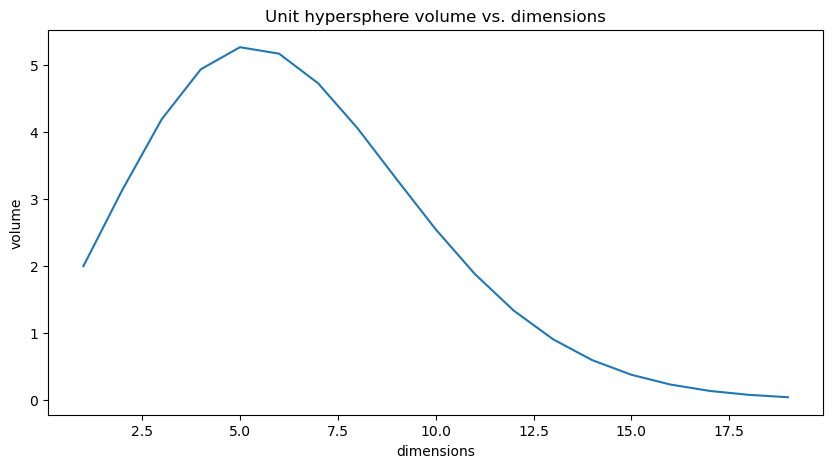
\includegraphics[width=0.8\textwidth]{TheorethicalFramework/ND-Laplace/Images/volume.png}
  \caption{Illustration of the decreasing volume while increasing the number of dimensions}
  \label{fig:curse-of-dimensionality}
\end{figure}

The noise decreases as the dimensions increase, increasing utility.
Hence, observing the behavior of privacy relative to utility is intriguing.
This behavior will be further emphasized in a later stage of this research.
\newpage
\subsection{Grid-remapping}
In the previous sections, we introduced the 2D, 3D, and nD Laplace mechanisms.
The current section will be used to formalize nD-Laplace with grid-remapping (disretization \& truncation) and introduce modifications to improve the mechanisms for clustering for n-dimensional data.

\subsubsection{Discretization and truncation} \label{theory:nd-laplace-truncation}
To recall the working of 2D and 3D-Laplace remapping, we give a short summary of section \todo{Add section refs}. The 2D version operates on a plane and approximates on a grid $G$, while the 3D version works in a sphere and approximates the data using a cuboid grid  $G_M$ (See Section \todo{Add ref})
Given a set of perturbed points $Z$ we can truncate the points that are outside the domain by remapping them to points within $G$ ($Z = X \cap G$) \citep{DBLP:journals/corr/abs-1212-1984}.
Here, $X$ represents other non-private data points reported locally by the same user. 
The following part aims at extending the theorems for 2D and 3D-Laplace for discritezation and truncation to n-dimensions. \newline

The theorems for 2D (See  Theorem\ref{theorem:discretization} and 3D-Laplace (See Theorem \ref{theorem:3d-discretization}} include a device precision. This variable is the hardware precision of a GPS provided by the user's device (e.g. a mobile phone). For the purpose of clustering, we omit this for the formulation of truncation with n-dimensions.

We extend the reasoning of Min et al. behind extending 2D-Laplace to 3D-Laplace as this applies to nD-Laplace as well. 
Let $v > w > h$ be a cuboid grid $G_c$, equal to the one provided by Min et al \citep{9646489}. 
We are be-able to extend this by providing a hypercube ($n$-cube) with n-dimensions denoted as $G_n = u_1, u_2, u_3 ... u_n$. This $n$-cube has $2^n$ sides, but can essentially be seen as a generalization of a 3-cube to $n$-dimensions \footnote{https://mathworld.wolfram.com/Hypercube.html}.
An issue arises with the definition of the grid-units, where Min et al. and Andres et al. both consider the possibility of unequal grid-units, for the purpose of generalisation \citep{9646489, DBLP:journals/corr/abs-1212-1984}.
However, for a $n$-cube this is generalisation is harder to justify, because \todo{Add reasoning}.
For this reason, we define $v, w, h = u_1$. We choose $u_1$, but in general this can be any given value $u \in G_n$. 
Another important property, is the maximum diameter defined as $r_M$ \citep{9646489}.
This property can also be converted to support n-dimensions, by calculating the diameter of $G_n$. 
This is the maximum distance between any pair of nodes  [HARARY1988277].:  
The Euclidean distance diameter is defined as (ref):
\begin{equation}
    d_e(G_n) = r_H = \sqrt{n}
\end{equation}

Where, $n$ is the amount of dimensions. 
\newpage  
Finally, we are be-able to establish our own theorem for the discretization and truncation of nD-Laplace:
\begin{theorem}
    Assume $u$ to be a side length, Let $G_u$ be an $n$-dimensional hypercube of $u$ size, Let $r_H < u$ and let $w = \frac{u^2}{r^2_H \cdot sin (\theta)} > \frac{u}{r_H}.$ Let $\epsilon, \epsilon' \in R^+$ such that \\
    $\epsilon' + \frac{1}{u} ln \frac{w + n \cdot e^{\epsilon' \cdot u}}{w - n \cdot e^{\epsilon' \cdot h}} \leq \epsilon$ \\
    Then $K\epsilon'$ satisfies $\epsilon$-geo-indistinguishability within range
    of $r_H$. That is to say, if $d_n(x, z)$ and $d_{euc}(x, x') \leq r_H$ then, 
      $K(x)(z) \leq e^{\epsilon \cdot d_{euc} (x, x')} \cdot K(x')(z)$ forall $x, x' \in X, z \in Z$ \citep{chatzikokolakis_constructing_2015}
\end{theorem}
Since we specify the hypercube to have equal sides of $u_i$, we are be-able to simplify the theorem.
%We use the proof provided by Min et al. in some extend by satisfying preliminary variables \citep{9646489}.
By satisfying the conditions for $r_H$ and $u$, we use the proof provided for 3-dimensions and use it for $n$-dimensions \citep{9646489}.
If we select a $u$ smaller then the max diameter $r_H$, we can satisfy $d_{euc}(x_n, x0) < r_H < u$. Which is according to the proof provided by Min et al.
Moreover, $w = \frac{u^2}{r_H^2 \cdot sin(\theta)} > \frac{u}{r_H}$ is also satisfied as the sizes of $G_n$ are equal. 
Given that these pre-conditions apply, we can reuse the proof from 3-dimensions for n-dimensions. \newline

The utility of this method depends on the number of grid cells in $G_n$ since a smaller distance will result in more frequent mapping to the surface of the grid.
When $\epsilon$ is very low (and thus $z$ is farther away from $x_0$), the data points are more likely to map to the grid surface (\ref{fig:3d-laplace-noise}, \ref{fig:3d-laplace-example}), and if the grid cells width is very high this impacts utility.
So, the number of grid cells could possibly the utility, but this comes at the cost of significantly increased space complexity. Also, when the number of dimensions increases, the number of grid cells grows quadratic. \newline

\subsubsection{Optimization}
To make grid-remapping practically possible with n-dimensions, the data structure has to be more efficient to search spatial data. For this purpose, we adopt the idea proposed by Chatzikokolakis et al. of using a kd-tree to search the grid efficiently \citep{chatzikokolakis_efficient_2017}.
Their research describes the theoretical utilization of a kd-tree for searching nearby points for a given point.
For this reason, we aim to apply this practically by using a kd-tree for the following tasks:
\begin{enumerate}
  \item Finding nearby points for $z \in G$ (Section: \ref{theory:grid-remapping}).
  \item Finding nearby points for $x \in X$ and $z \in Z$ (Section: \ref{theory:optimal-remapping}).
\end{enumerate}
The usage of kd-tree does not impact any privacy guarantee provided in the previous section. It is just a more efficient way of searching in n-dimensional spatial structures. Also, for visualization purposes, this section will primarily focus on 2D data. \newline
The next section explains the concept and underlying idea of kd-trees.
Then, we delve into its application for grid remapping.
Finally, we expand this to a practical application
\newpage
\subsubsection*{Kd-trees} \label{theory:kd-trees}
A kd-tree algorithm can search a grid for nearby points \citep{bentley_multidimensional_1975}.
It can do so by recursively splitting the grid into a binary tree to search for grid coordinates \citep{washington_k-d_2002}.
In addition, it preserves spatial information of the data so it can be utilized to find nearby points using Euclidean distance (nearest neighbor search).
The following example provides an idea of how this works (Figure \ref{fig:kd-tree-theory}):
\begin{figure}[H]
  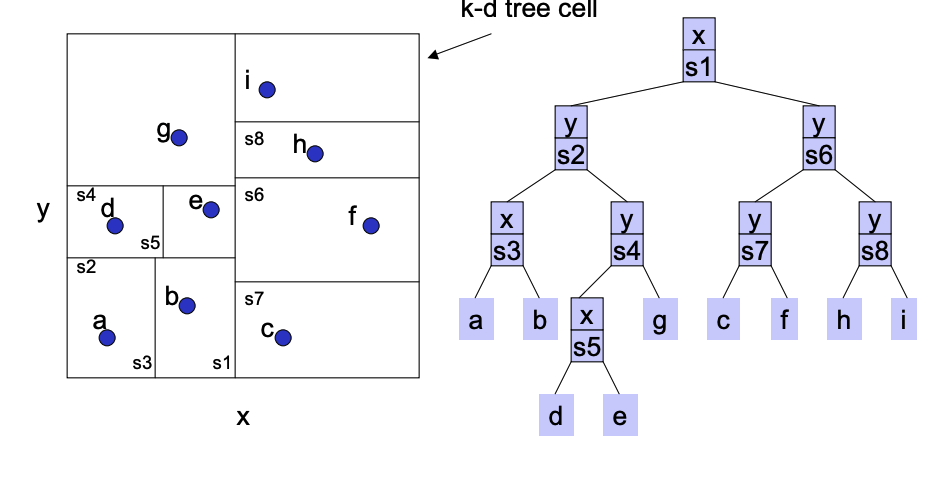
\includegraphics[width=0.8\textwidth]{TheorethicalFramework/ND-Laplace/Images/kd-tree-part1.png}
  \caption{Representation of constructing a kd-tree with 2 dimensions \citep{washington_k-d_2002}.}
  \label{fig:kd-tree-theory}
\end{figure}
Take, for example, the 2D Laplace algorithm that utilizes a plane (left side).
The data points can be divided based on their x and y coordinates.
Each coordinate becomes a node in the binary tree, and the grid is divided based on these splits.
The binary tree allows us to search the grid efficiently.
An example of this is provided in the following image (Figure \ref{fig:kd-tree-searching-theory}):
\begin{figure}[H]
  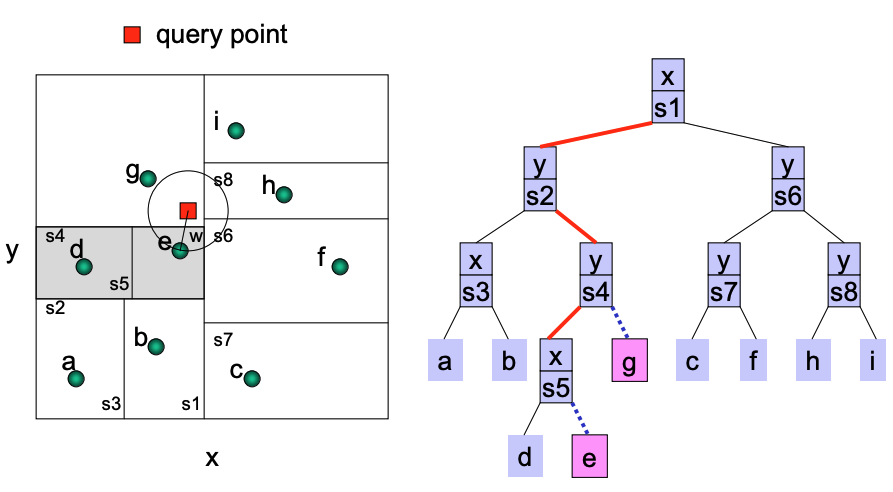
\includegraphics[width=0.8\textwidth]{TheorethicalFramework/ND-Laplace/Images/kd-tree-part2.png}
  \caption{Representation of searching a kd-tree with 2 dimensions \citep{washington_k-d_2002}.}
  \label{fig:kd-tree-searching-theory}
\end{figure}
In the example, we are searching for all points that fall within the radius of a random query point.
The most significant advantage is that this dramatically reduces the complexity of searching.
Constructing the kd-tree costs equal to grid-remapping $O(kn)$, where $k$ is the number of dimensions and $n$ is the dataset size.
But, searching for the nearest neighbor is a logarithmic function with time complexity of $O(\log n)$ \citep{washington_k-d_2002} (See Figure \ref{theory:big-o-graph} for an overview of the Big-O notation).
This approach is a significant improvement over searching manually, which would have the same complexity as constructing the tree.

\subsubsection{Grid remapping with kd-tree} \label{theory:grid-remapping}
The kd-tree search method is beneficial for the optimizations we are striving for.
This optimization extends grid-remapping for 2d \citep{DBLP:journals/corr/abs-1212-1984} and 3d data \citep{9646489} to n-dimensions. \newline
We have illustrated the three steps required for this below:
\begin{figure}[H]
  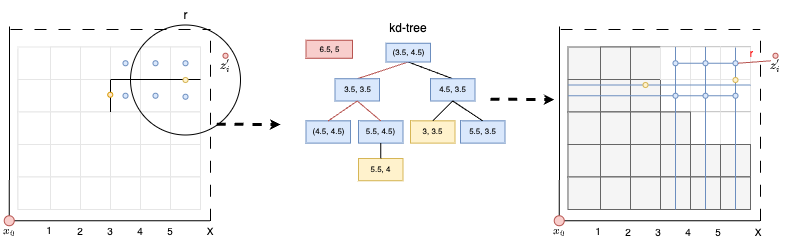
\includegraphics[width=1\textwidth]{TheorethicalFramework/ND-Laplace/Images/KD-tree.png}
  \caption{Representation utilizing a kd-tree for applying grid-remapping \citep{DBLP:journals/corr/abs-1212-1984}}
  \label{fig:kd-tree}
\end{figure}
%When using a kd-tree to search for a data point $z_i$, the algorithm begins with an unbalanced binary tree.
%The root is split by the x-axis, and since 4.5 is greater than 3.5, we go to the right.
%This means that we no longer need to consider the left (greyed out) part of the grid.
%We continue traversing the tree until we find the nearest point based on Euclidean distance.
For easy visualization, the process shown above is with 2-dimensional data.
However, this can be extended to n-dimensional using the kd-tree optimization.
The goal is to remap a perturbed point $z \in Z$, outside the original domain $X$, to the closest point in $X$ or $G$ \citep{DBLP:journals/corr/abs-1212-1984}.

Firstly, a grid is generated, where each (blue) point represents the center of a grid cell.
Together, these centroids form the grid dataset, denoted as $G$.
The yellow points and $x_i$ are part of the original collection, denoted as $X$.
Here, $r$ represents the radius used to generate a private version of the data point $x_i$, named $z_i$, based on 2D-Laplace.
In the illustration, you can observe that $z_i$ falls outside the original domain of $X$, so it needs to be remapped.
We accomplish this by utilizing the nearest-neighbor search from the kd-tree algorithm, allowing us to search in $X \cup G$.
Using this algorithm, we can effectively remap point $z \in Z$ to either $X$ or $G$ based on the closest Euclidean distance (Algorithm \ref{alg:grid-remapping-laplace} and Algorithm \ref{alg:find-outside-domain-laplace}).

Although the methodology works for scaling grid-remapping for n-dimensional data, it can still cause scalability issues.
It still does not scale well with the number of dimensions and a more significant number of grid cells.
Therefore, we are looking for a solution that might work better in practice

\begin{algorithm}[H]
  \caption{Algorithm for finding points outside the domain of $X$.}
  \begin{algorithmic}
    \Require $x \in X$  
    \Require $z \in Z$ 
    %\State $tree \gets KDTree(X)$ \Comment construct a KDTree from the original data.
    \State $X_{domain} \gets \Call{KDTree::query}{Z}$ \Comment find the closest points.
    \State $X_{features} \gets \Call{List::getfeatures}{X}$ 
    \State $X_{outside-domain} \gets []$
    \For{$feature \in X_{features}$} 
    \If{$feature \leq \Call{X::min}{Z} $}
    \State $\Call{row::append}{X_{outside-domain}}$
    \EndIf
    \If{$feature \geq \Call{X::max}{Z} $}
    \State $\Call{row::append}{X_{outside-domain}}$
    \EndIf
    \EndFor
    \State \Return $X_{outside-domain}$ 
  \end{algorithmic}
  \label{alg:find-outside-domain-laplace}
\end{algorithm}
\begin{algorithm}[H]
  \caption{Algorithm for generating and remapping to a grid.}
  \begin{algorithmic}
    \Require $x \in X$  \Comment original dataset
    \Require $z \in Z$ \Comment perturbed dataset
    \Require $grid$ \Comment grid structure ($n * m$)
    %\State $tree \gets KDTree(X)$ \Comment construct a KDTree from the original data.
    %\State $X_{domain} \gets$ \Call{KDTree::query}{$Z$} \Comment find the closest points.
    \State $d_{X} = dist(Z, X)$ \Comment euclidean distances
    \State $d_{grid} = dist(Z, grid)$ 
    \State $Z_{out-domain} \gets FindPointsOutsideDomainX(X, Z)$ \Comment Algorithm \ref{alg:find-outside-domain-laplace}
    \State $grid_{tree} \gets KDTree(grid)$ 
    \State $grid_{mask} \gets KDTree::query(Z)$ \Comment find indices of $z \in Z$ that are closeby grid cells.
    \State $Z_{grid-mask} \gets Z_{out-domain} \cup d_{grid} < d_{X}$ \Comment All points $z \in Z$ that are closeby grid cells and are outside domain.
    \State $Z` \gets Z[grid[grid_{mask}][Z_{grid-mask}]]$ \Comment combinate masks to set appropiate indexes to $g \in grid$.
    \State \Return $Z`$
  \end{algorithmic}
  \label{alg:grid-remapping-laplace}
\end{algorithm}
\newpage
\subsection{Density remapping} \label{theory:optimal-remapping}
As discussed, the remapping will be performance intensive to provide good utility, so we adopt the optimal remapping \citep{chatzikokolakis_efficient_2017}.
This thesis will refer to this as density remapping because this better explains the application.

According to the grid-remapping methodology, a point $z_i$ is mapped to the center of the grid cell.
The utility is improved by reducing the distance between $z_i$ and $x_i$, as this is closer to the original data point.
But, to consider the privacy of the data, this can only be done if there is enough indistinguishability between $z_i$ and $x_i$.
To this end, we adopt the remapping approach of Chatzikokolakis et al. to remap based on the data density \citep{chatzikokolakis_efficient_2017}.
The remapping algorithm works on the idea of crowded places \ref{2d:optimizing}, with the intuition that a crowded place leverages indistinguishability by crowdedness (density) \citep{chatzikokolakis_efficient_2017}.  \newline

The approach is visualized using the following figure:
\begin{figure}[H]
  \includesvg{TheorethicalFramework/ND-Laplace/Images/master-thesis-Page-12.svg}
  \label{fig:optimal-remapping}
  \caption{Representation of density remapping \citep{chatzikokolakis_efficient_2017}}
\end{figure}
The first step is calculating $B_r(z_i)$, which refers to all the data points within the radius $r$ around the data point $z_i$ \citep{chatzikokolakis_efficient_2017}.
Then, the algorithm collects the data points around $x_i$, again using $r$, to determine the density of $x_i$.
This is the convex hull (collection) of all the original data points within the radius $r$ around $x_i$ and is denoted as $Q_r (x_i)$.
Finally, we obtain $Q_r$ which is a union of $Q_r (x_i)$ and $B_r(z_i)$.
Now that we have the sets of points around $x_i$ and $z_i$, we can calculate the density \citep{chatzikokolakis_efficient_2017}:
\begin{equation}
  \forall x'_i \in Q_r \quad \sigma(x_i) = \frac{w(x'_i)e^{-\epsilon d(x'_i, z_i)}}{\sum{_{q\in Q_r} w(q)e^{-\epsilon d(q, z_i)}}}
  \label{eq:optimal-remapping-formula-1}
\end{equation}
$w(q)$ is the weight of a point $q \in Q_r$, and $w(x_i)$ the weight of a point $x_i \in X$.
Here, the weight can be a point of interest \citep{chatzikokolakis_efficient_2017}.
But, in the context of our study, we consider the points within $r$ of $q$ or $x_i$ to be the weight.

In equation \ref{eq:optimal-remapping-formula-1}, the $w(x)$ and $w(q)$ are normalization factors for estimating the likelihood of a point $x'_i$ being close to $z_i$ and $q$ being close to $z_i$.
So, this remapping is according to the original definition of the 2D Laplace \gls{pdf} definition \ref{eq:polar-laplace-pdf}.
The outcome of the formula is a collection of values that indicate the degree of density $sigma(x_i)$.
The new value $z'_i$ is calculated by taking the mean of the $sigma(x_i)$ \citep{chatzikokolakis_efficient_2017}:
\begin{equation}
  z_i' = \sum_{x'_i \in Q_r} \sigma(x'_i) * x'_i
  \label{eq:optimal-remapping-formula-2}
\end{equation}
By applying this formula, the new $z_i'$ is closer to $x_i$ to minimize the expected loss of utility \citep{chatzikokolakis_efficient_2017}.
Much like the 2D and 3D Laplace methods, which use the likelihood of a point $z_i$ being close to $x_i$ \citep{DBLP:journals/corr/abs-1212-1984, 9646489}.
%The first step is to calculate the coefficients for each point $x \in X$ by multiplying the density $\sigma(x)$ with the original point $x$.

%The probability that $z'$ will be closer to $x$ is higher, and this probability is calculated based on the original value $x \in X$ to first determine the coefficient.
%Finally, the new $z'$ is calculated by taking the mean value of $\sigma(x)$ \citep{chatzikokolakis_efficient_2017}.
%As described by chatzikokolakis et al., the 
%Chatzikokolakis et al's work considers a prior set of data point $Q \in R^n$.
%Which are other data points that belong to the user.
%We are interested in the data points that are within the radius $r$ around $z$.
%This is denoted as $B_r(z)$, which is the vector of all points within radius $r$ around $z$.
%In addition to this, there is also a $Q_r$ that is a convex hull of all nearby points.
%Hence, this is described as $Q_r = B_r \cap Q$.
%The final intuition here is that $r$ is automatically generated based on crowdedness (see circle inside figure \ref{fig:optimal-remapping}).
%The last step is to take the mean value of $\sigma(x)$.
%Unfortunately, optimal remapping is not possible for users that do not have sufficient data (e.g. new users).
%The remapping is not applied for these users and is also not applied for $z$ if it is within the domain of $X$.
\begin{algorithm}[H]
  \caption{Algorithm to implement the density remapping of $z \in Z$ to be in the domain of $x \in X$}
  \begin{algorithmic}[1]
    \Require $x \in X$
    \Require $z \in Z$
    \Require $epsilon$
    \Ensure $z' \in Z$
    \State $Z' = FindRemappedPoints(Z)$ \Comment Algorithm: \ref{alg:find-outside-domain-laplace}
    \State $tree \gets KDTree(X)$
    \For{$z' \in Z'$}
    \State $r = \Call{FindRadius}{(z')}$ \Comment Get original radius $r$.
    \State $X_r \gets \Call{KDTree::query}{x}$ \Comment find $q \in X$ around $x$ with radius $r$.
    \State $B_r \gets \Call{KDTree::query}{z'} $
    \State $\sigma(x) = []$
    \State $Q_r = \gets X_r \cap B_r$
    \State $w_x = \Call{Length}{X_r, B_r}$ \Comment weight is simply adding density of $X_r$ and $B_r$.
    \For{$q \in Q_r$}
    \State $q \gets \Call{KDTree::query}{q}$
    \State $w_q = \Call{Length}{Q_r}$ \Comment $w_q$ is the density of each point $q$ within $Q_r$.
    \State $\sigma(w_x) \gets \Call{Remap}{w_x, \epsilon}$ \Comment Equation \ref{eq:optimal-remapping-formula-1}.
    \State $\sigma(x) \gets \Call{Append}{\sigma}$ \Comment add to the list $\sigma(x)$.
    \EndFor
    \State $z' \gets \Call{Average}{\sigma(x)}$ \Comment Equation: \ref{eq:optimal-remapping-formula-2}.
    \EndFor
  \end{algorithmic}
  \label{alg:optimal-remapping-laplace}
\end{algorithm}

\begin{itemize}
  \item 1: Receives all the points $z \in Z$ that are outside the domain of $X$.
  \item 2: Constructs a KDTree from the original data $X$, so it can be queried.
  \item 3: Receives the original privacy radius $r$ that was used to generate $z$ from $x$.
  \item 4: $X_r$ is the set of points $x \in X$ that are within the radius $r$ of $x$.
  \item 5: $B_r$ is the set of points $z \in Z$ that are within the radius $r$ of $z$.
  \item 7: $w_x$ is the "popularity" of $x$ and $z$, for the number of points is counted within the radius $r$.
  \item 12: $w_q$ is the weight of each point $q \in Q_r$, so $q$ is re-assigned to be the number of points within the radius $r$ of $q$.
\end{itemize}

\newpage
The equation for density remapping \ref{eq:optimal-remapping-formula-1} was created for 2-dimensional data.
However, we aim to use this same approach for 3-dimensional and n-dimensional data.
To do so, we first revisit the \gls{pdf} for 3D-Laplace, which was defined using this Equation: \ref{eq:3d-laplace-pdf}.
Few modifications are necessary, as the normalization factor $A$ is now defined using Equation: \ref{eq:optimal-remapping-formula-1}.
\todo[inline]{Formulate the definition of $A$}
\todo[inline]{Check if this can be extended to nD-Laplace}

\newpage
\subsection{Putting it together: kd-Laplace}
Now that we have defined everything, we can write the algorithm in a step-by-step manner:
\begin{algorithm}[H]
    \caption{Full algorithm for perturbing training data for nD-clustering using planar/2D-Laplace \citep{DBLP:journals/corr/abs-1212-1984}}\label{alg:rq1}
    \begin{algorithmic}
      \Require $x \in X$  \Comment 2D array of points
      \Require $l \in R^ +$
      
      \State \Return Z
    \end{algorithmic}
    \label{alg:nd-laplace}
  \end{algorithm}

It is important to note that with the introduction of this algorithm, it is no longer a non-interactive method, as the data points now interact with each other.
Therefore, we expect the introduction of optimal grid remapping with kd-tree will bring more utility \citep{wang_comprehensive_2020, xiongComprehensiveSurveyLocal2020}.
The introduction of the kd-tree is also why we present our method as \textit{kd-Laplace}, where $k$ is the number of dimensions.
%\todo[inline]{Also refactor this}

%\subsection{Extending to $d_x$-privacy}
%\todo[inline]{Find if this is possible}

%Constructing elastic distinguishability metrics for location privacy
\newpage

\subsection{Mechanism flowchart}
All formulas and theories are established for 2D, 3D, and nD-Laplace, so the mechanism design applies to all three variants:
\begin{figure}[h]
  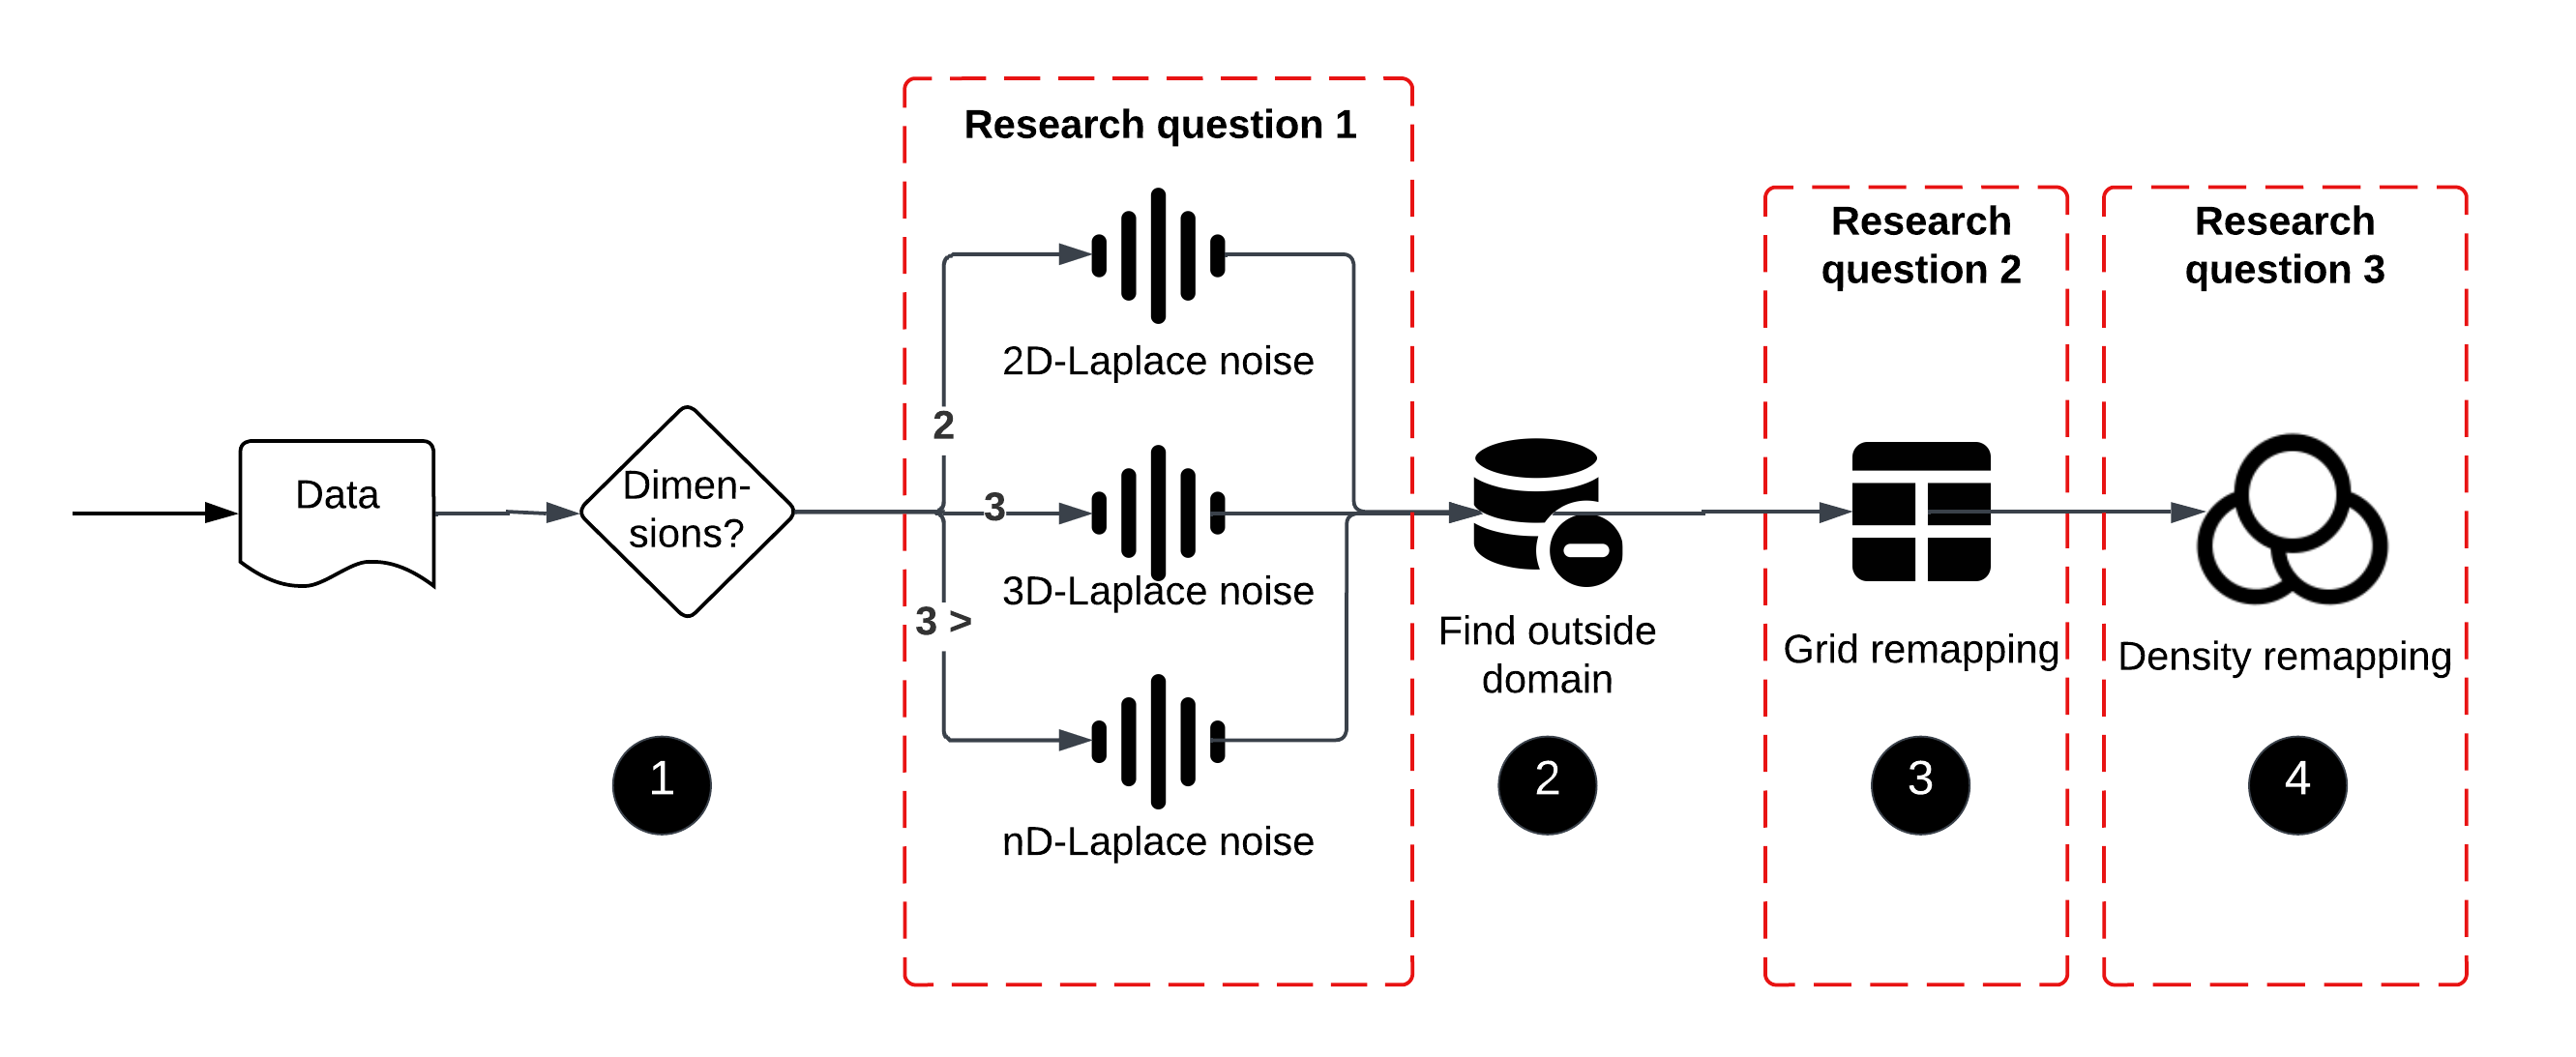
\includegraphics[width=1.1\textwidth]{TheorethicalFramework//ND-Laplace//Images/Thesis-nd - final-mechanism-design.png}
  \caption{Non-interactive mechanism design for nD-Laplace.}
  \label{fig:final-mechanism-design}
\end{figure}
%\todo[inline]{Modify to density-nD-Laplace \& nD-Laplace for image reporting}
For easy navigation, we provide a list of all algorithms:
\begin{enumerate}
  \item Based on the number of dimensions, the algorithm decides the correct Laplace mechanism to use:
        \begin{itemize}
          \item 2D-Laplace:  \ref{alg:2d-laplace}
          \item 3D-Laplace: \ref{alg:3d-laplace}
          \item nD-Laplace: \ref{alg:nd-laplace}
        \end{itemize}
  \item Find points outside domain: \ref{alg:find-outside-domain-laplace}
  \item Grid remapping: \ref{alg:grid-remapping-laplace}
  \item Density remapping: \ref{alg:optimal-remapping-laplace}
\end{enumerate}
\added{In addition, relevant research questions are incorporated into the architecture overview.
These questions are covered in chapter \ref{chapter:methodology}}.
\subsubsection{Practical example}
The shape of the dataset is necessary for the usefulness of clustering.
With our algorithm, there are four different shapes/variants of the dataset.
For example, this has been visualized using a 3D dataset based on the heart dataset (\ref{datasets-section}).
Our mechanism aims to provide privacy and preserve the dataset's shape to benefit the utility of clustering.
Grid remapping and optimal remapping are used to achieve this goal.

\begin{figure}[H]
  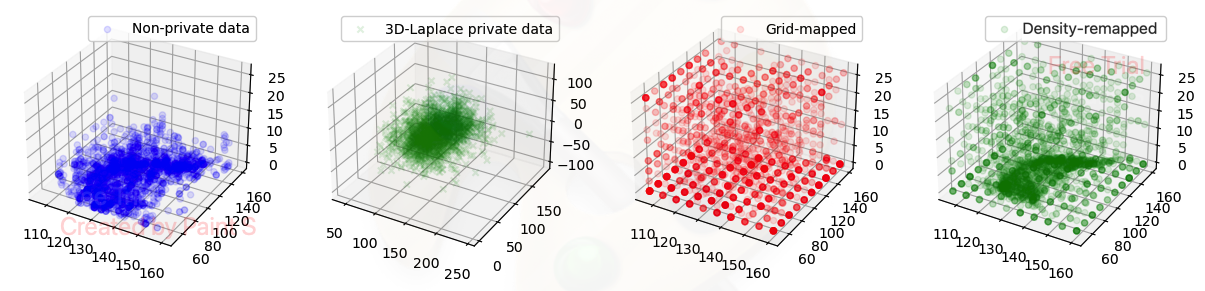
\includegraphics[width=1.1\textwidth]{TheorethicalFramework/ND-Laplace/Images/optimal-remapping-example.png}
  \caption{Example of optimal remapping for the 3D-dataset: Cardiotocography. The example shows the different steps of the mechanism in sequence for a dataset perturbed with a privacy budget of 0.1.}
\end{figure}

\begin{enumerate}
  \item Dataset: the blue dots represent the original dataset without any modifications.
  \item Adding noise: the green crosses represent the dataset after adding noise; for this particular example, this is 3D-Laplace (Algorithm \ref{alg:3d-laplace}):
        As can be observed, the data is generated from the center, causing many data points to fall outside the original domain of the dataset.
  \item Grid-remapping: the red dots represent the dataset after grid-remapping (Algorithm \ref{alg:grid-remapping-laplace})
        After performing the grid remapping algorithm, all points within the domain are plotted.
        However, the original shape of the data is mostly lost.
        This makes it challenging to cluster the data as was possible with the original data.
  \item Optimal-remapping: the green dots represent the dataset after optimal-remapping (Algorithm \ref{alg:optimal-remapping-laplace}).
        After completing the previous step, the data points are again remapped based on the (original) density.
        This results in restoring the original shape of the data and, consequently, the clusters.
\end{enumerate}


\chapter{Attacks on privacy} \label{section: MIA}
This chapter is devoted to investigating and evaluating attacks on machine learning models.
Differential privacy protects the centrally stored dataset from leaking sensitive information.
Therefore, assessing the mechanism's privacy is best measurable using common attacks \citep{jayaraman_evaluating_nodate}.
In this context, we evaluate attacks that explicitly uncover training data from a privately trained model.
We consider two types of attacks:
\begin{enumerate}
  \item \textbf{Reconstruction attack}:  An adversary could reconstruct training data from a given (classifier) model using a reconstruction attack. The goal of the adversary is to reconstruct a secret bit $b$ from a row, by producing random data that agrees on this secret bit $b$. \citep{dwork_exposed_2017}. 
  \item \textbf{Membership inference attack}: An adversary attempts to infer whether a data point was used for training. With this attack, an adversary attempts to infer the training data $x \in X$ (member) from a given data point $z \in Z$ (non-member).
%An attack model that plays a significant role in machine learning is \gls{mia}.

\end{enumerate}
The knowledge of the attacker (adversarial knowledge) is an important factor to consider.
This knowledge can be divided into white-box and black-box approaches \citep{hu_membership_2022}.
\begin{enumerate}
  \item \textbf{White-box}: The attacker has all the needed data. Including target model parameters or the architecture \citep{hu_membership_2022}.
  \item \textbf{Black-box}: The attacker has limited information, like training data distribution and the trained model \citep{hu_membership_2022}.
\end{enumerate}
%The concept of reconstruction attacks predates differential privacy, as this principle also gave rise to the idea of database privatization \citep{dinur_revealing_2003}.
 %\newline
%A general reconstruction attack for our use-case is the attribute inference attack \citep{dwork_exposed_2017} or model inference \citep{rigaki_survey_2021}, but both terms are essentially the same \citep{jegorova_survey_2022}. 
%Differential privacy aims to introduce sufficient noise to mitigate the risk of these attacks \citep{dwork_exposed_2017,jayaraman_evaluating_nodate}.
%Assessing the privacy leakage of our model can be effectively accomplished by employing attribute/membership inference techniques.
Both reconstruction and membership attacks serve the purpose of assessing the effectiveness of \gls{dp} mechanisms to preserve privacy. 
However, the membership attack has an attack-model that is easier to generalize by inferring training data, while the reconstruction attack depends much more on data-properties.
This thesis has many different datasets, and as both types of attacks serve the same purpose, \gls{mia} is the better fit. \newline
Therefore, the focus of evaluating \gls{dp} will rely primarily on \gls{mia} and the next section is used to evaluate different attacks for this attack type.
%So, for the purpose of estimating privacy leakage \gls{mia} is the better option.
%Therefore, the \gls{mia} is more

%The next section is used to formalize/explain a few common attacks.

\section{Membership inference attacks}
The attack happens exclusively on supervised learning models, which predict labels or probabilities.
Most attacks on models trained on a centralized dataset occur during the inference phase, where the trained model is used to make predictions. \citep{rigaki_survey_2021}.
This is also why we are primarily interested in this phase, as we are not using a distributed learning model.

The most well-known member inference attack is training shadow models \citep{rigaki_survey_2021}.
In this attack, an attacker trains multiple models.
These models do not necessarily have to be the same as the original model, and the focus is mainly on the data input/output.
It is a black-box attack, but the attacker often needs knowledge of the data distribution to create a good shadow dataset \citep{rigaki_survey_2021}.

One of the earlier works that used this attack was Shokri et al. \citep{shokri_membership_2017}.
This idea is based on the confidentiality percentages of classification model outputs. Presumably the model gives higher scores to the data on which it was trained (overfitting) in comparison to other data. This information is misused by the attacker to reconstruct the original training data.

 Let $y = f_{target(x)}$ be the prediction confidence of a classification model, then the membership probability is calculated as \citep{shokri_membership_2017}: 
\begin{equation}
    Pr(x, y) \in D^{train}_{target}
\end{equation}
Which is the probability of that input $x$ belongs to the target dataset that was used to generate the target dataset $f_{target}$ \citep{shokri_membership_2017}.
To execute the attack, the attacker trains so-called shadow models $f^i_{shadow}()$, and each of them are trained on dataset that is comparable to the training dataset and combined to infer training information:
\begin{figure}[H]
  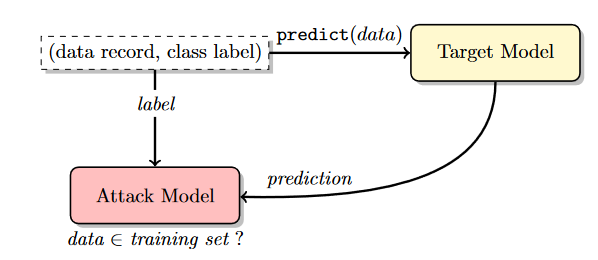
\includegraphics[width=0.5\textwidth]{TheorethicalFramework/AttacksOnPrivacy/shadow-models-mi.png}
  \caption{Black-box MIA attack on a machine learning model \citep{shokri_membership_2017}}
\end{figure}

Another approach to a black-box attack was introduced by Peng et al. and only considers that the attacker has access to the already trained model.
They first rescale the probabilities using temperature scaling to compensate for overconfident models \citep{peng_unsupervised_nodate}:
\begin{equation}
    R_i(h_k(x);T) = \frac{exp(log(h^i_k(x))/T}{\sum_j{exp(log(h^j_k(x))/T}}
\end{equation}
Here, the $h(x)$ denotes the probability distribution of $x$, which tells the chance of $x$ being a certain classification/label. Peng et al. then calculate the top-$k$ features $h_k$ and eliminate the smaller values. 
The formula $R_i$ is are the re-scaled probabilities,  to be more suitable for clustering using temperature scaling, where $T$ is the scaling parameter.  They the fit a K-Means model, resulting in two clusters: training and test data \citep{peng_unsupervised_nodate}.
%Access to only the output of the model is a typical characteristic of black-box attacks. If the attacker also knows architecture, for example, it is referred to as a white-box attack.

%The above attacks do rely on the model to also provide the confidence or probabilities of the predictions.
%This information is often unavailable, so Choquette-Choo et al. introduced a label-only attack.
%While the existing models exploit MIA's probability output, they rely solely on labels \citep{choquette-choo_label-only_2021}.
%They use the "HopSkipJump" attack, a so-called decision-based attack \citep{chen_hopskipjumpattack_2020}.
%Choquette-Choo et al. consider a more semi-black-box approach, for which the attacker still requires access to a subset of the original training data and the trained model.
%Another paper using "HopSkipJump" requires only the trained model and achieves higher accuracy using an approach with random data \citep{li_membership_2021}. \newline






%If the data is fed with real data the score is higher than similar data, which means the real data can be inferred \citep{shokri_membership_2017,jayaraman_evaluating_nodate}
%A white-box setting requires a lot of adversarial knowledge for training the shadow models.
%The black-box settings only take the prediction as input and decide if it is a (non-) member \citep{hu_membership_2022}.
%To conclude on this, there are many methods for MIA and in that regard, the black-box approaches look the most promising.
%They require less setup and there is plenty of black-box approaches score with a success rate of 70\% and 80\%.
%For our use case, however, it is harder to establish an MIA; as we focus mainly on clustering.
%Anyhow, it is possible if we consider a semi-supervised approach where we consider the cluster labels as ground truth.
%%Differential privacy is proposed as a wmay of solving the inference attack for both white-box and black-box \citep{hu_membership_2022}.
%%However, it is hard to find a way to protect privacy and utility as well, so it depends heavily on the privacy budget.

\newpage


\mycomment{A practical implementation of the attack was provided by Fredrikson et al. as a way to infer sensitive features \citep{fredrikson_model_2015}.
To accomplish this, they used a decision tree attack, a white-box approach, as they also accessed the count of instances for each decision tree branch.
They also considered a black-box approach with access only to the target model (ML-as-a-service in this example).
% Finally, they showed that if the attacker can capture a single output label, they can reproduce the original data with high confidence \citep{fredrikson_model_2015}.
The attack targets gradient descent, which is used to optimize the input data of an attack to mimic the original data.
It has only been shown to work on a neural network for face identification images (named MIFace) \citep{fredrikson_model_2015}, but it could be extended to another machine learning classifier if it uses gradient descent (e.g. Support Vector Machines) \citep{nicolae_adversarial_2019}.
%Most other comparable work focus almost exclusively on neural networks [decristofaroOverviewPrivacyMachine2020a, jegorovaSurveyLeakagePrivacy2022].
 Yeom et al. proposed a membership inference attack, which can also be utilized for attribute inference in a white-box setting.
The attribute inference attack follows a similar methodology, wherein the target model is queried to assess the loss of synthetic data based on adversarial knowledge.
Repeating the process, the attack identifies and selects the value with the highest prior probability, incorporating membership information \citep{yeom_privacy_2018,jayaraman_are_2022}.
Evaluating the effectiveness of such attacks is challenging, as it relies on the correlation between attributes, irrespective of whether the data belongs to the training or test dataset \citep{zhao_feasibility_2021}.
Therefore, Yeom et al. focus on the similarity between membership/attribute- inference and combine them to evaluate the attribute inference attack \citep{yeom_privacy_2018}. \newline}

%using available code implementations \citep{nicolae_adversarial_2019}.
\newpage
%\section{Model inversion attack}
%\todo[inline]{Do research for this attack}

% \section{Poison attack}
%\textbf{Reconstruction attacks:}
%Another attack that is a threat, especially to differential privacy is a reconstruction attack.
%This attack is also more known as the attribute inference attack and is more focused on the data itself than machine learning models \citep{rigaki_survey_2021}. 

%\textbf{Model extraction attacks:}
%The final attack that is considered, is the model extraction attack.
%This attack consists of the attacker being able to reconstruct and gather information about the original model.

% Jayaraman et al. evaluate inference attacks and differential privacy and express a metric called "privacy leakage"  \citep{jayaraman_evaluating_nodate}.



\section{Attack evaluation} \label{theory:attack-evaluation}
In this section, we evaluate the membership inference attack and evaluate it as it is the most appropriate for this study (See previous chapter).
We assess whether differential privacy provides protection against the attack and discuss how this can be measured.
\subsection{Member inference attacks}
% Research
Most current research for \gls{mia} is evaluated for neural networks \citep{rigaki_survey_2021}.
A tiny percentage evaluates this attack for supervised learning, with the majority using classification with decision trees.
Most studies have used a black-box approach \citep{rigaki_survey_2021} for these attacks.
This approach is not surprising, as these attacks have a high success rate and pose a greater risk of exploitation.

% Metrics
Introducing differential privacy reduces the impact of a member inference attack \citep{rigaki_survey_2021,hu_membership_2022}.
This is because the input to the model is perturbed.
While it is still possible to retrieve the training data, the leaked privacy is significantly reduced.
A simple but effective way to measure the privacy leakage is by calculating the accuracy of correctly predicting membership by the adversary \citep{choquette-choo_label-only_2021}.

Yeom et al. created a metric specifically for membership inference attacks which can be measured using an "membership advantage" \citep{yeom_privacy_2018}.
This metric describes the percentage of privacy compromised during a member inference attack.
This metric is calculated by subtracting the \gls{fpr} from the \gls{tpr}.
The \gls{tpr} represents the number of correctly predicted member data (training data), and the \gls{fpr} represents the number of correctly predicted non-member data.
Although these metrics are commonly applied in the literature for \gls{mia}, they do not provide enough information \citep{carlini_membership_2022}.
Both metrics do not consider the imbalance between the \gls{tpr} and \gls{fpr}.
The metric should emphasize the \gls{tpr}, as this is the percentage of correctly predicted member data.
Therefore, they propose to use a ROC curve to show the effectiveness of a membership inference attack \citep{carlini_membership_2022}. \newline

% Final remark
In conclusion, the attacks that use \gls{mia} are all (mis)using supervised machine learning.
However, in this study, we use clustering algorithms.
Therefore, a semi-supervised approach can be used, as illustrated in Figure \ref{figure:MIA-semi-supervised}.
\newpage
\begin{figure}[h]
  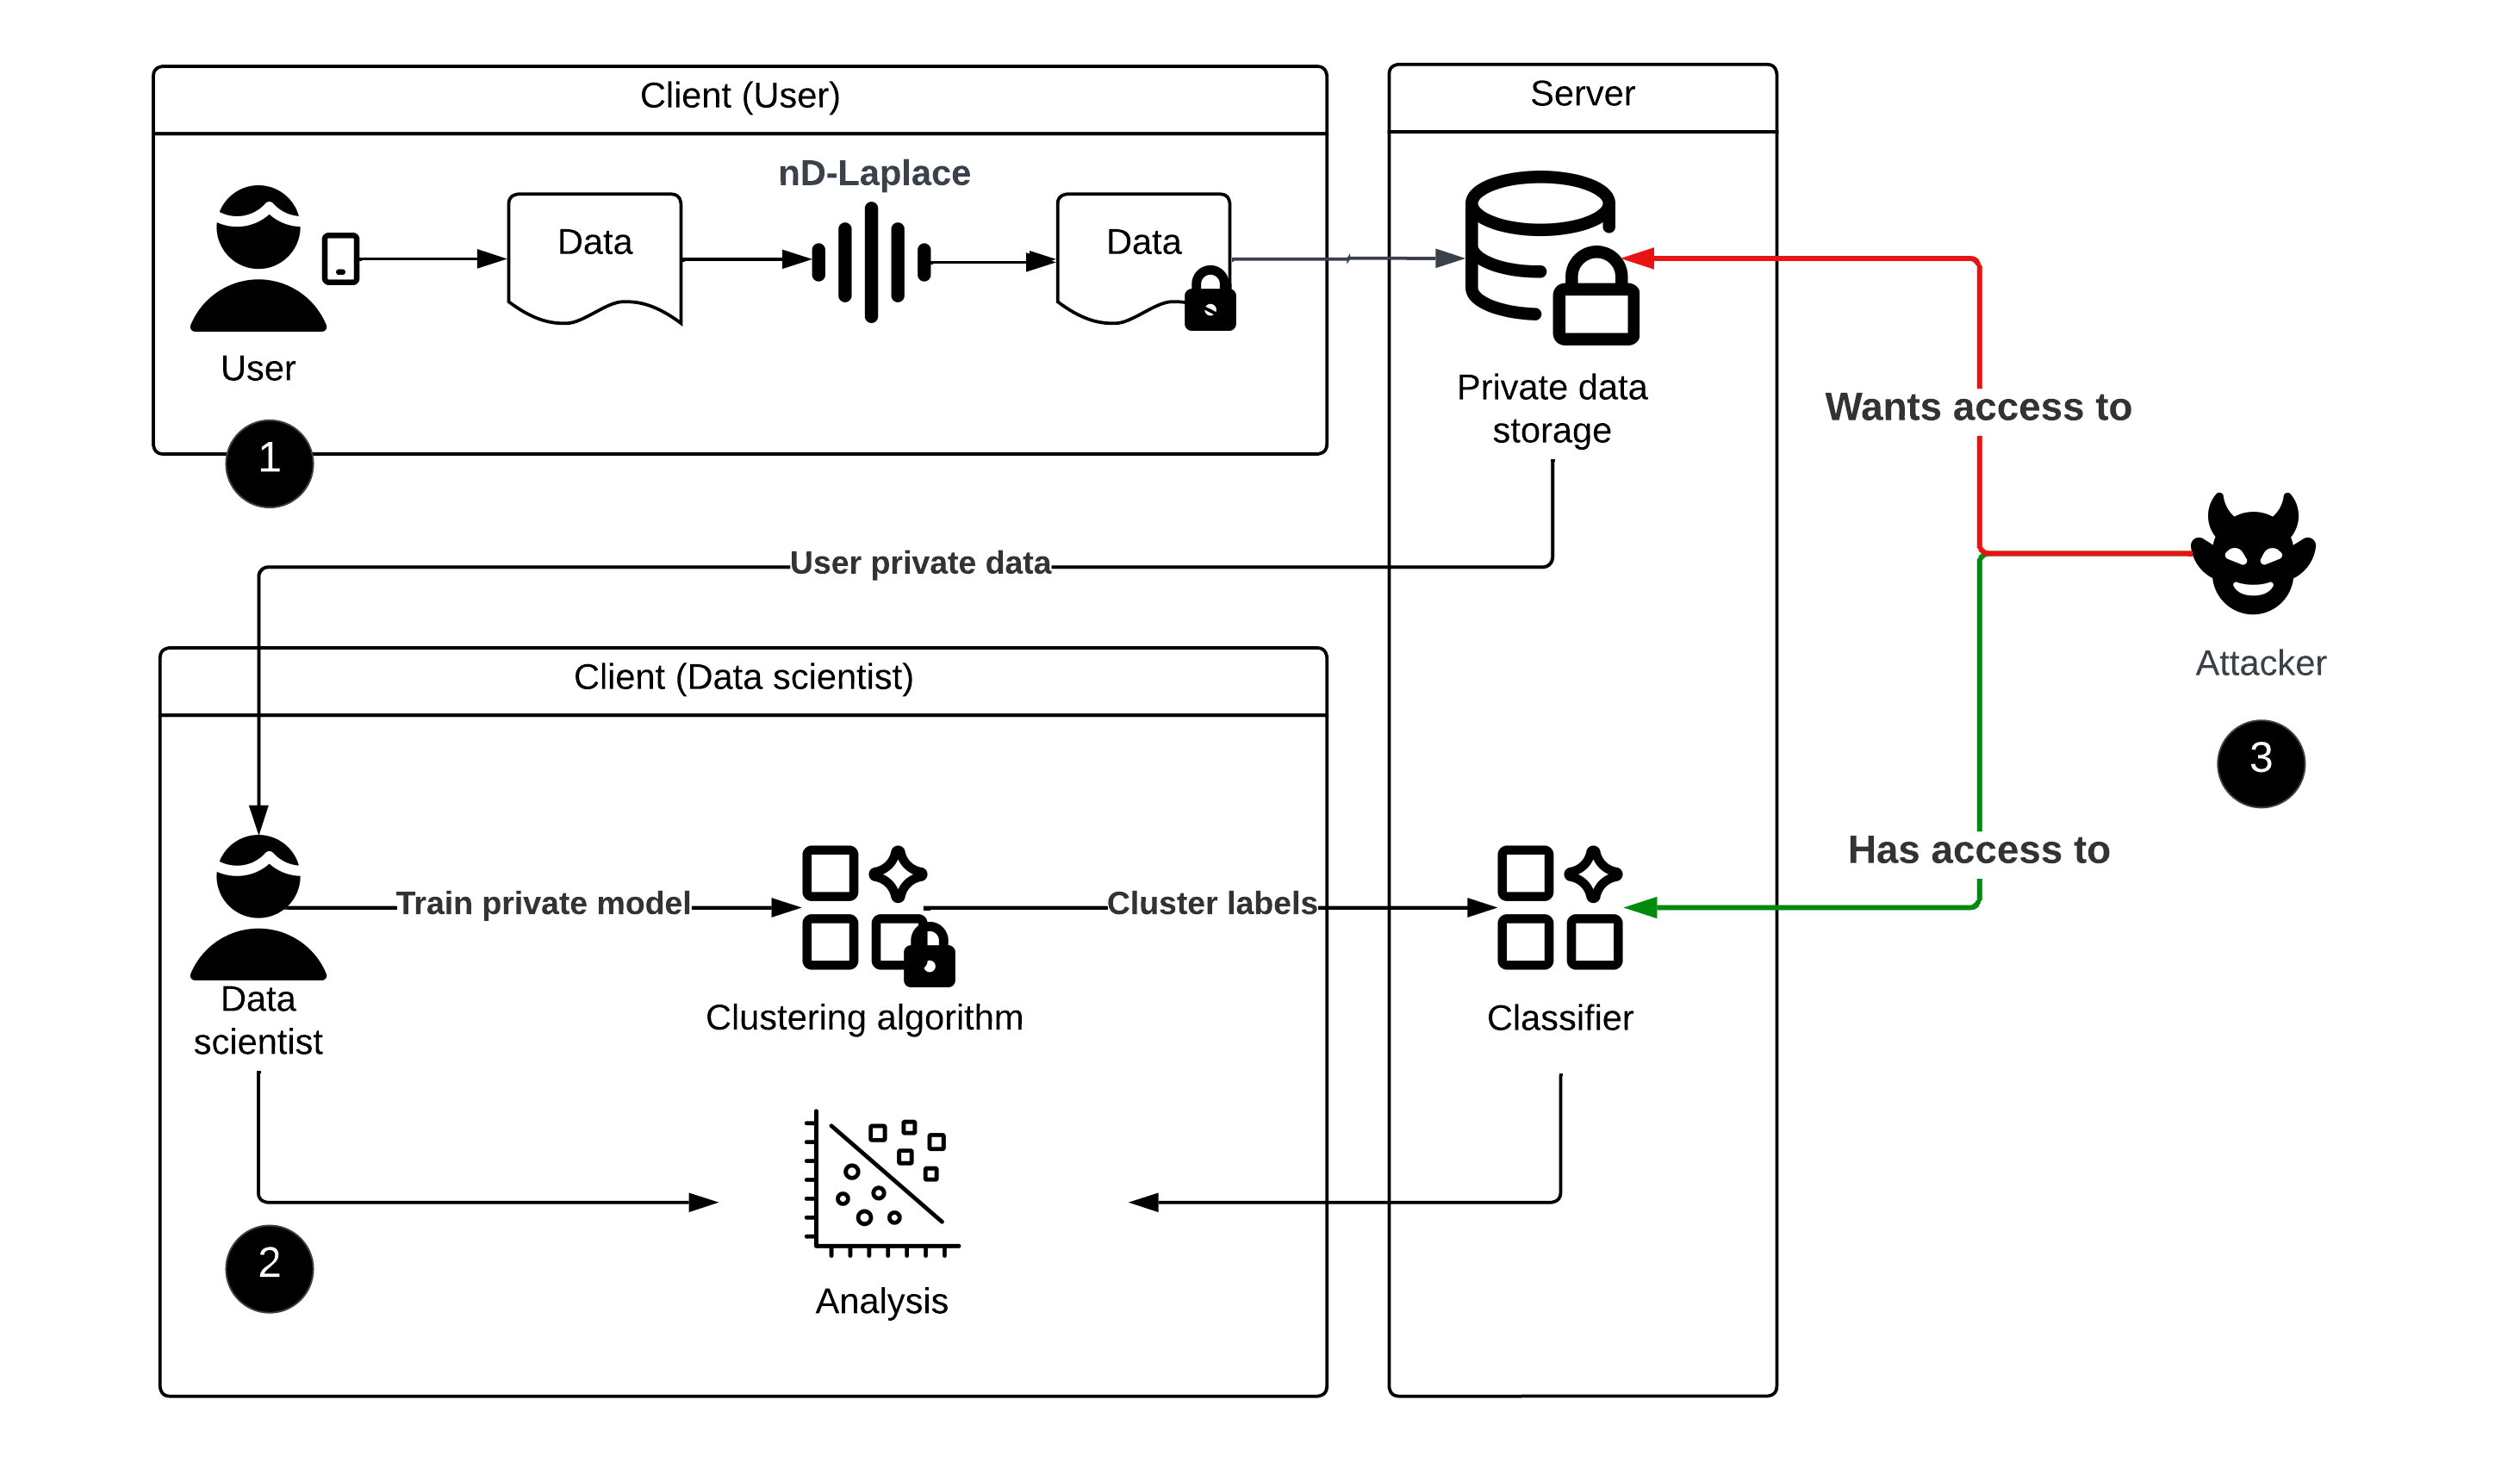
\includegraphics[width=1\textwidth]{TheorethicalFramework/Differential privacy/master-thesis-MIA.png}
  \caption{Semi-supervised black-box approach to execute a member inference attack.}
  \label{figure:MIA-semi-supervised}
\end{figure}

\begin{enumerate}
  \item The user uses a client (e.g., mobile app), where the nD-Laplace noise is added locally to the data.
  \item A data scientist trains the clustering algorithm with the privatized data.
        Therefore, the clustering algorithm's input and output (labels) are private.
        These labels are used to train a classifier (semi-supervised setup).
  \item The attacker wants access to the private data on the server.
        In this approach, the attacker has access to the classifier on the server (black-box setting).
        So, the attacker can use the classifier's output to conduct a \gls{mia}.
\end{enumerate}

\chapter{Methodology}

To gain insights into the proposed methods for researching the appliance of (ND)-Laplace for cluster algorithms we conducted experiments.
The experiment results are used to evaluate our method against other literature.
In this chapter we explain:
\begin{enumerate}

  \item Datasets
  \item Environmental setup.
  \item For each research question: Description of the different experiments.
  \item For each research question: Results.
\end{enumerate}

\section{Datasets}
For this research, we will use a synthetic dataset for all three research questions.
% Please add the following required packages to your document preamble:
% \usepackage{booktabs}
\begin{table}[h]
  \begin{tabular}{@{}lllll@{}}
    \toprule
    Records & Centers & Dimensions & Standard deviation & Research \\ \midrule
    200     & 4       & 2          & 0.60               & RQ 1     \\ \bottomrule
  \end{tabular}
\end{table}

Research question 3 uses a "real-world" dataset to properly assess the different dataset properties that are the subject of this research question.
\todo[inline]{Describe datasets}

\section{Environmental setup}
\todo[inline]{Describe the exact environment details}
\section{Experiment setup}
\subsection{Research question 1}
We propose several solutions for open issues based on the theoretical framework. \newline
\textbf{Choosing r: } Based, on the idea of chatzikokolakis et al. to lower the size of the radius if the place is crowded, we can do the same with clustering.
For this, we could use a metric like the standard division.
This metric increases based on clutteredness of the data, which allows us to generate a radius $r$ automatically regardless of domain.
Therefore, we depend on the configurability of epsilon entirely on privacy level $l$.
We define this metric as:
\todo[inline]{Standard deviation * 2}
\todo[inline]{Image example}

\textbf{Truncation: }
\subsection{Research question 2}
\subsection{Research question 3}
\section{Results}
\subsection{Research question 1}
\subsection{Research question 2}
\subsection{Research question 3}
\newpage
\chapter{Results}
This chapter aims to present the results to the reader.
As indicated in the methodology, we tested four mechanisms (three variants of kd-Laplace and Piecewise) for their utility and privacy.
\begin{enumerate}
  \item Cluster utility: Visualise the utility of kD-Laplace and Piecewise for 2/3/n-dimensional data.
        The results are displayed using a line diagram, using \gls{ami} and \gls{sc}.
  \item Mechanism utility: Visualise the utility of kD-Laplace and Piecewise using a heatmap plot.
        The results for each dimension and privacy budget are provided for only the \gls{ami} score.
  \item Mechanism privacy: Visualise the privacy of kD-Laplace and Piecewise using a heatmap plot.
        The results for each dimension and privacy budget are provided for only the adversary advantage and privacy distance.
  \item Mechanism comparison: Visualise the comparison between the variants of kD-Laplace and Piecewise.
        The results for each mechanism \& variant are provided using a bar-plot for the \gls{ami} score (utility) and the adversary advantage (privacy).
\end{enumerate}
All results are reported for each dataset (See methodology: \ref{datasets-section}) separately.
\section{Cluster utility}
The results below display the difference in external and internal utility for the three clustering algorithms using the kd-Laplace and Piecewise mechanisms.
The x-axis shows the privacy budget, and the y-axis shows the \gls{ami}.
Please refer to the plots in the appendix for the same scores for kD-Laplace variants (See \ref{appendix:results-mechanism-utility}).
\newpage
\subsection{2-dimensional data}
\begin{figure}[H]
  \centering
  \caption{\textbf{AMI (top) and SC (bottom) for the kD-Laplace and Piecewise mechanisms for the 2-dimensional data seeds-dataset}}
  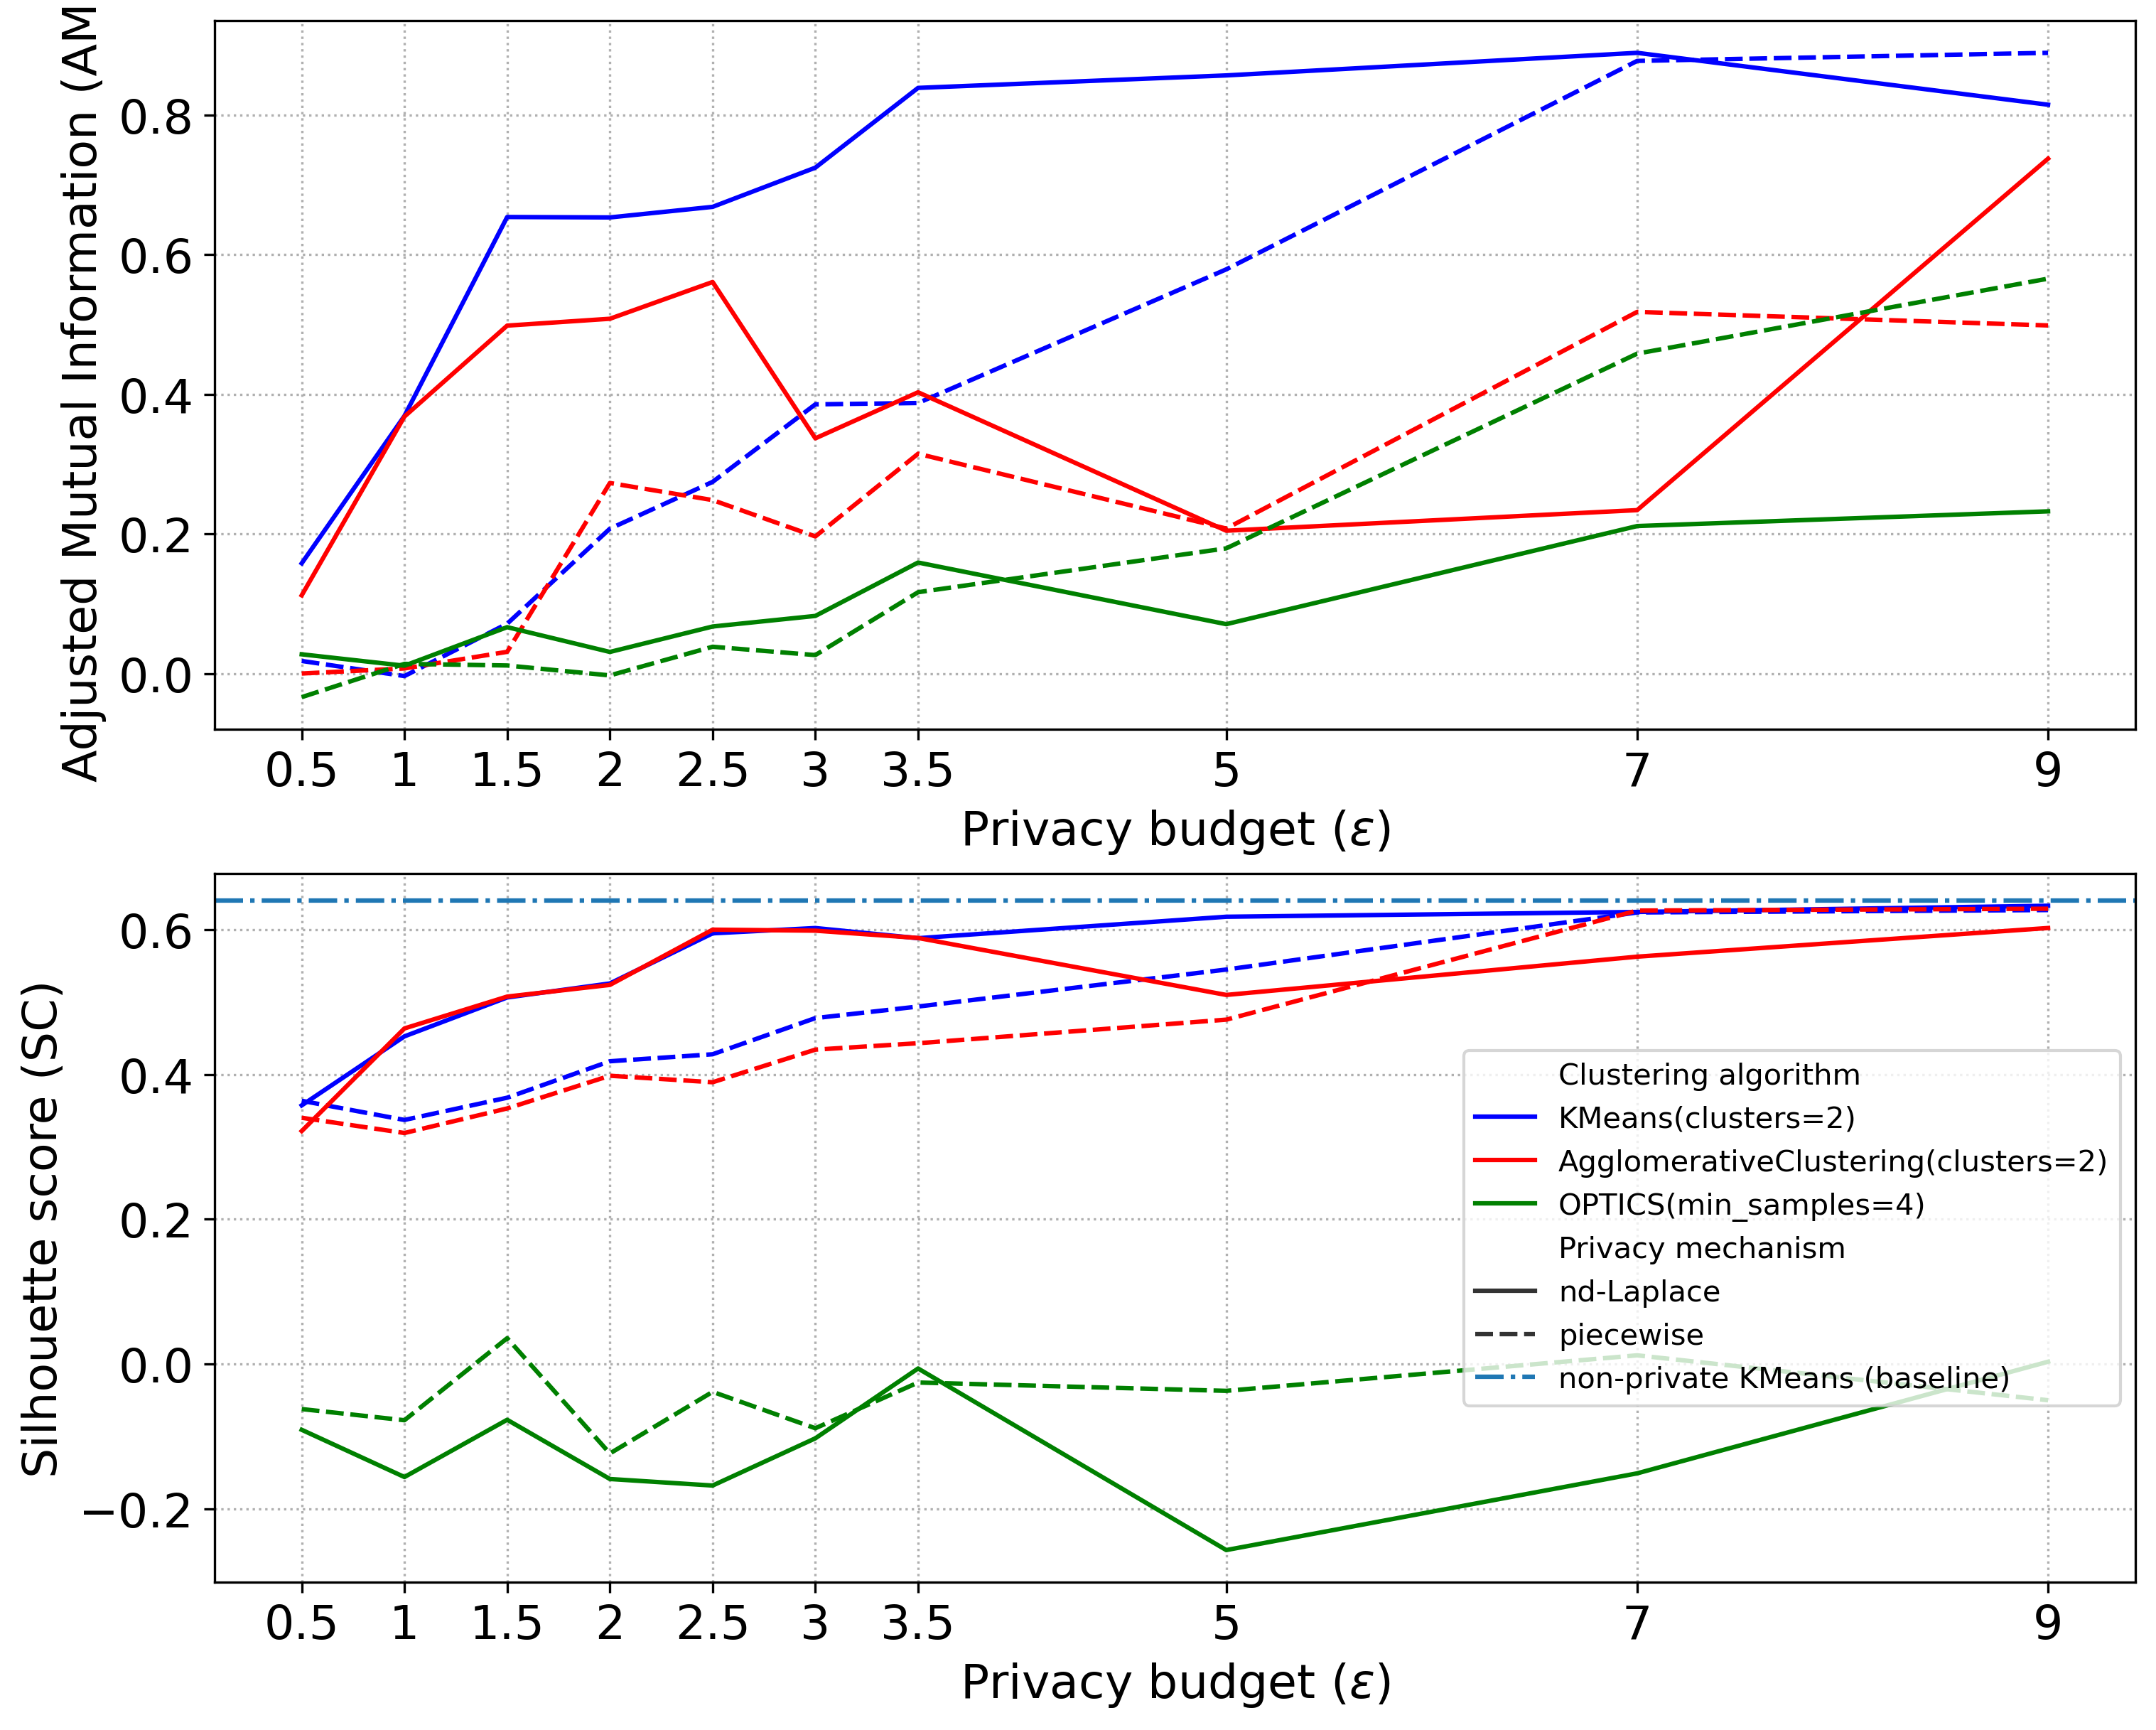
\includegraphics[width=0.8\textwidth]{Results/nd-laplace/nd-Laplace/seeds-dataset/ami-and-sc_2_dimensions.png}

  \label{fig:validation-seeds-dataset_comparison_2d-laplace}
\end{figure}
%The above plots show the AMI and ARI scores for the seeds-dataset with kd-laplace/grid/optimal (left-side) and piecewise (right-side).
The Piecewise mechanism excels in Adjusted Mutual Information (\gls{ami}) at a privacy budget (epsilon) of 9, while the nd-Laplace mechanism is superior for other epsilon values. K-Means consistently outperforms other clustering algorithms, though only marginally over \gls{ag}, and both yield similar silhouette coefficient (\gls{sc}) scores. The underperformance of the OPTICS algorithm across both mechanisms, comparable only to the AP algorithm under Piecewise, suggests its potential limitations in these configurations.
\newpage
The plot shows that nD-Laplace performs better for lower epsilons. Which is likely due to the mechanism also considering the shape (distance) of the data, so the Piecewise mechanism proportionally adds more noise. But, then we would expect OPTICS to score better. Therefore, we visualize this behaviour:
\begin{figure}[H]
    \centering
    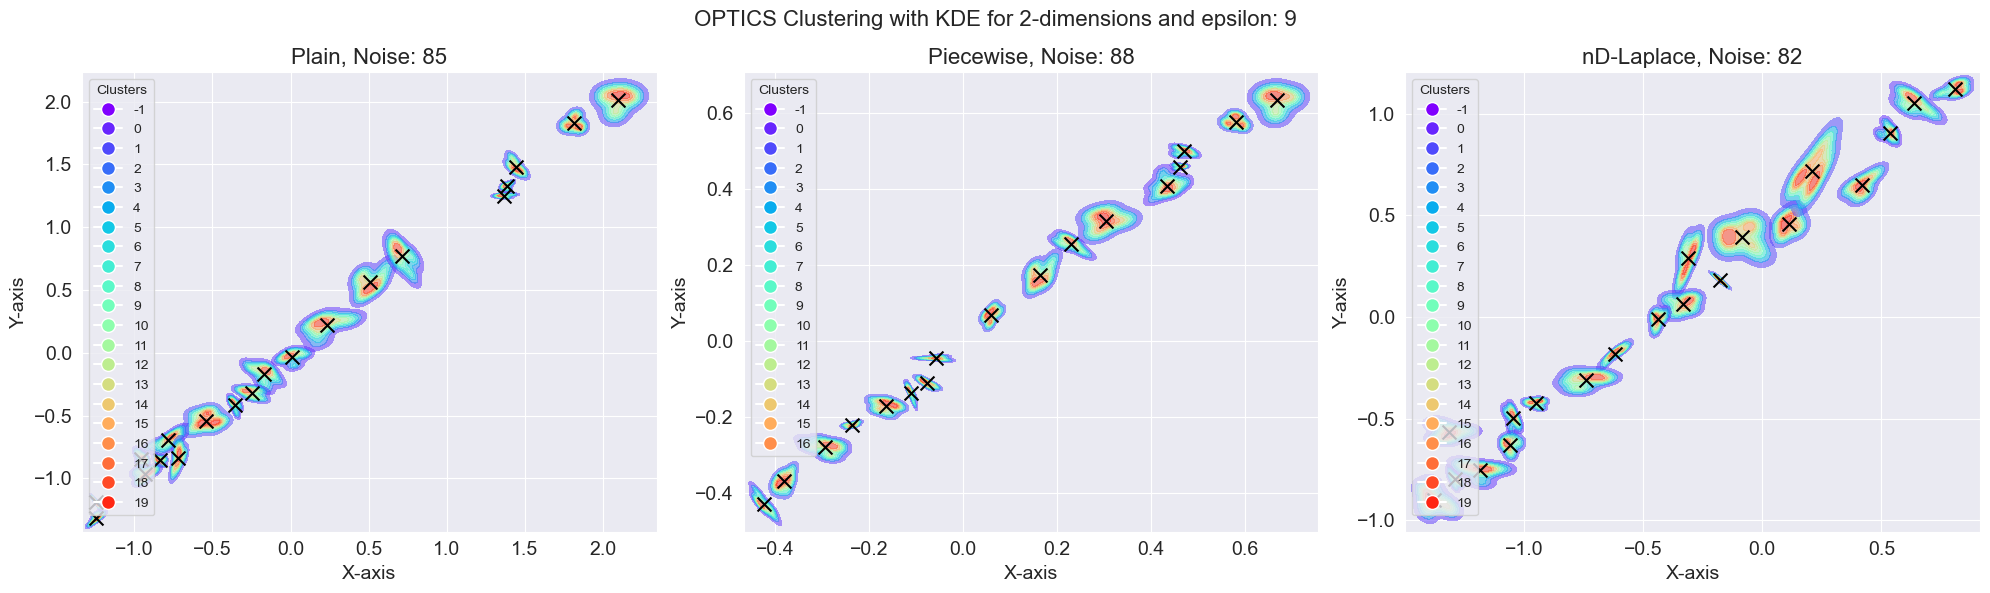
\includegraphics[width=1\linewidth]{Discussion/behaviour-2d-seeds-dataset&optics.png}
    \caption{Evaluating OPTICS for seeds-dataset 2-dimensional data (epsilon 9)}
    \label{fig:evaluate-optics-seeds-dataset-2d-9eps}
\end{figure}
The plot above illustrates the kernel density of core points chosen by the OPTICS algorithm for data with an epsilon value of 9. Clusters within the Plain and Piecewise datasets are compact and exhibit linear alignment, suggesting a distinct data distribution or directional noise stemming from the Piecewise mechanism. Conversely, the nD-Laplace clusters are more scattered, indicating that its noise impacts data uniformly across all directions.

Furthermore, the noise level is concerning. According to Schubert et al. (2017) \citep{schubert_dbscan_2017}, the noise should range between 1\% and 30\%. However, the OPTICS algorithm we employed indicates an average noise level of 40\%, pointing to a potential problem with the algorithm's implementation. Additionally, the number of clusters reported is notably high.


\newpage
\begin{figure}[H]
  \centering
  \caption{\textbf{AMI (top) and SC (bottom) for the nD-Laplace mechanism for the 2-dimensional data heart-dataset}}
  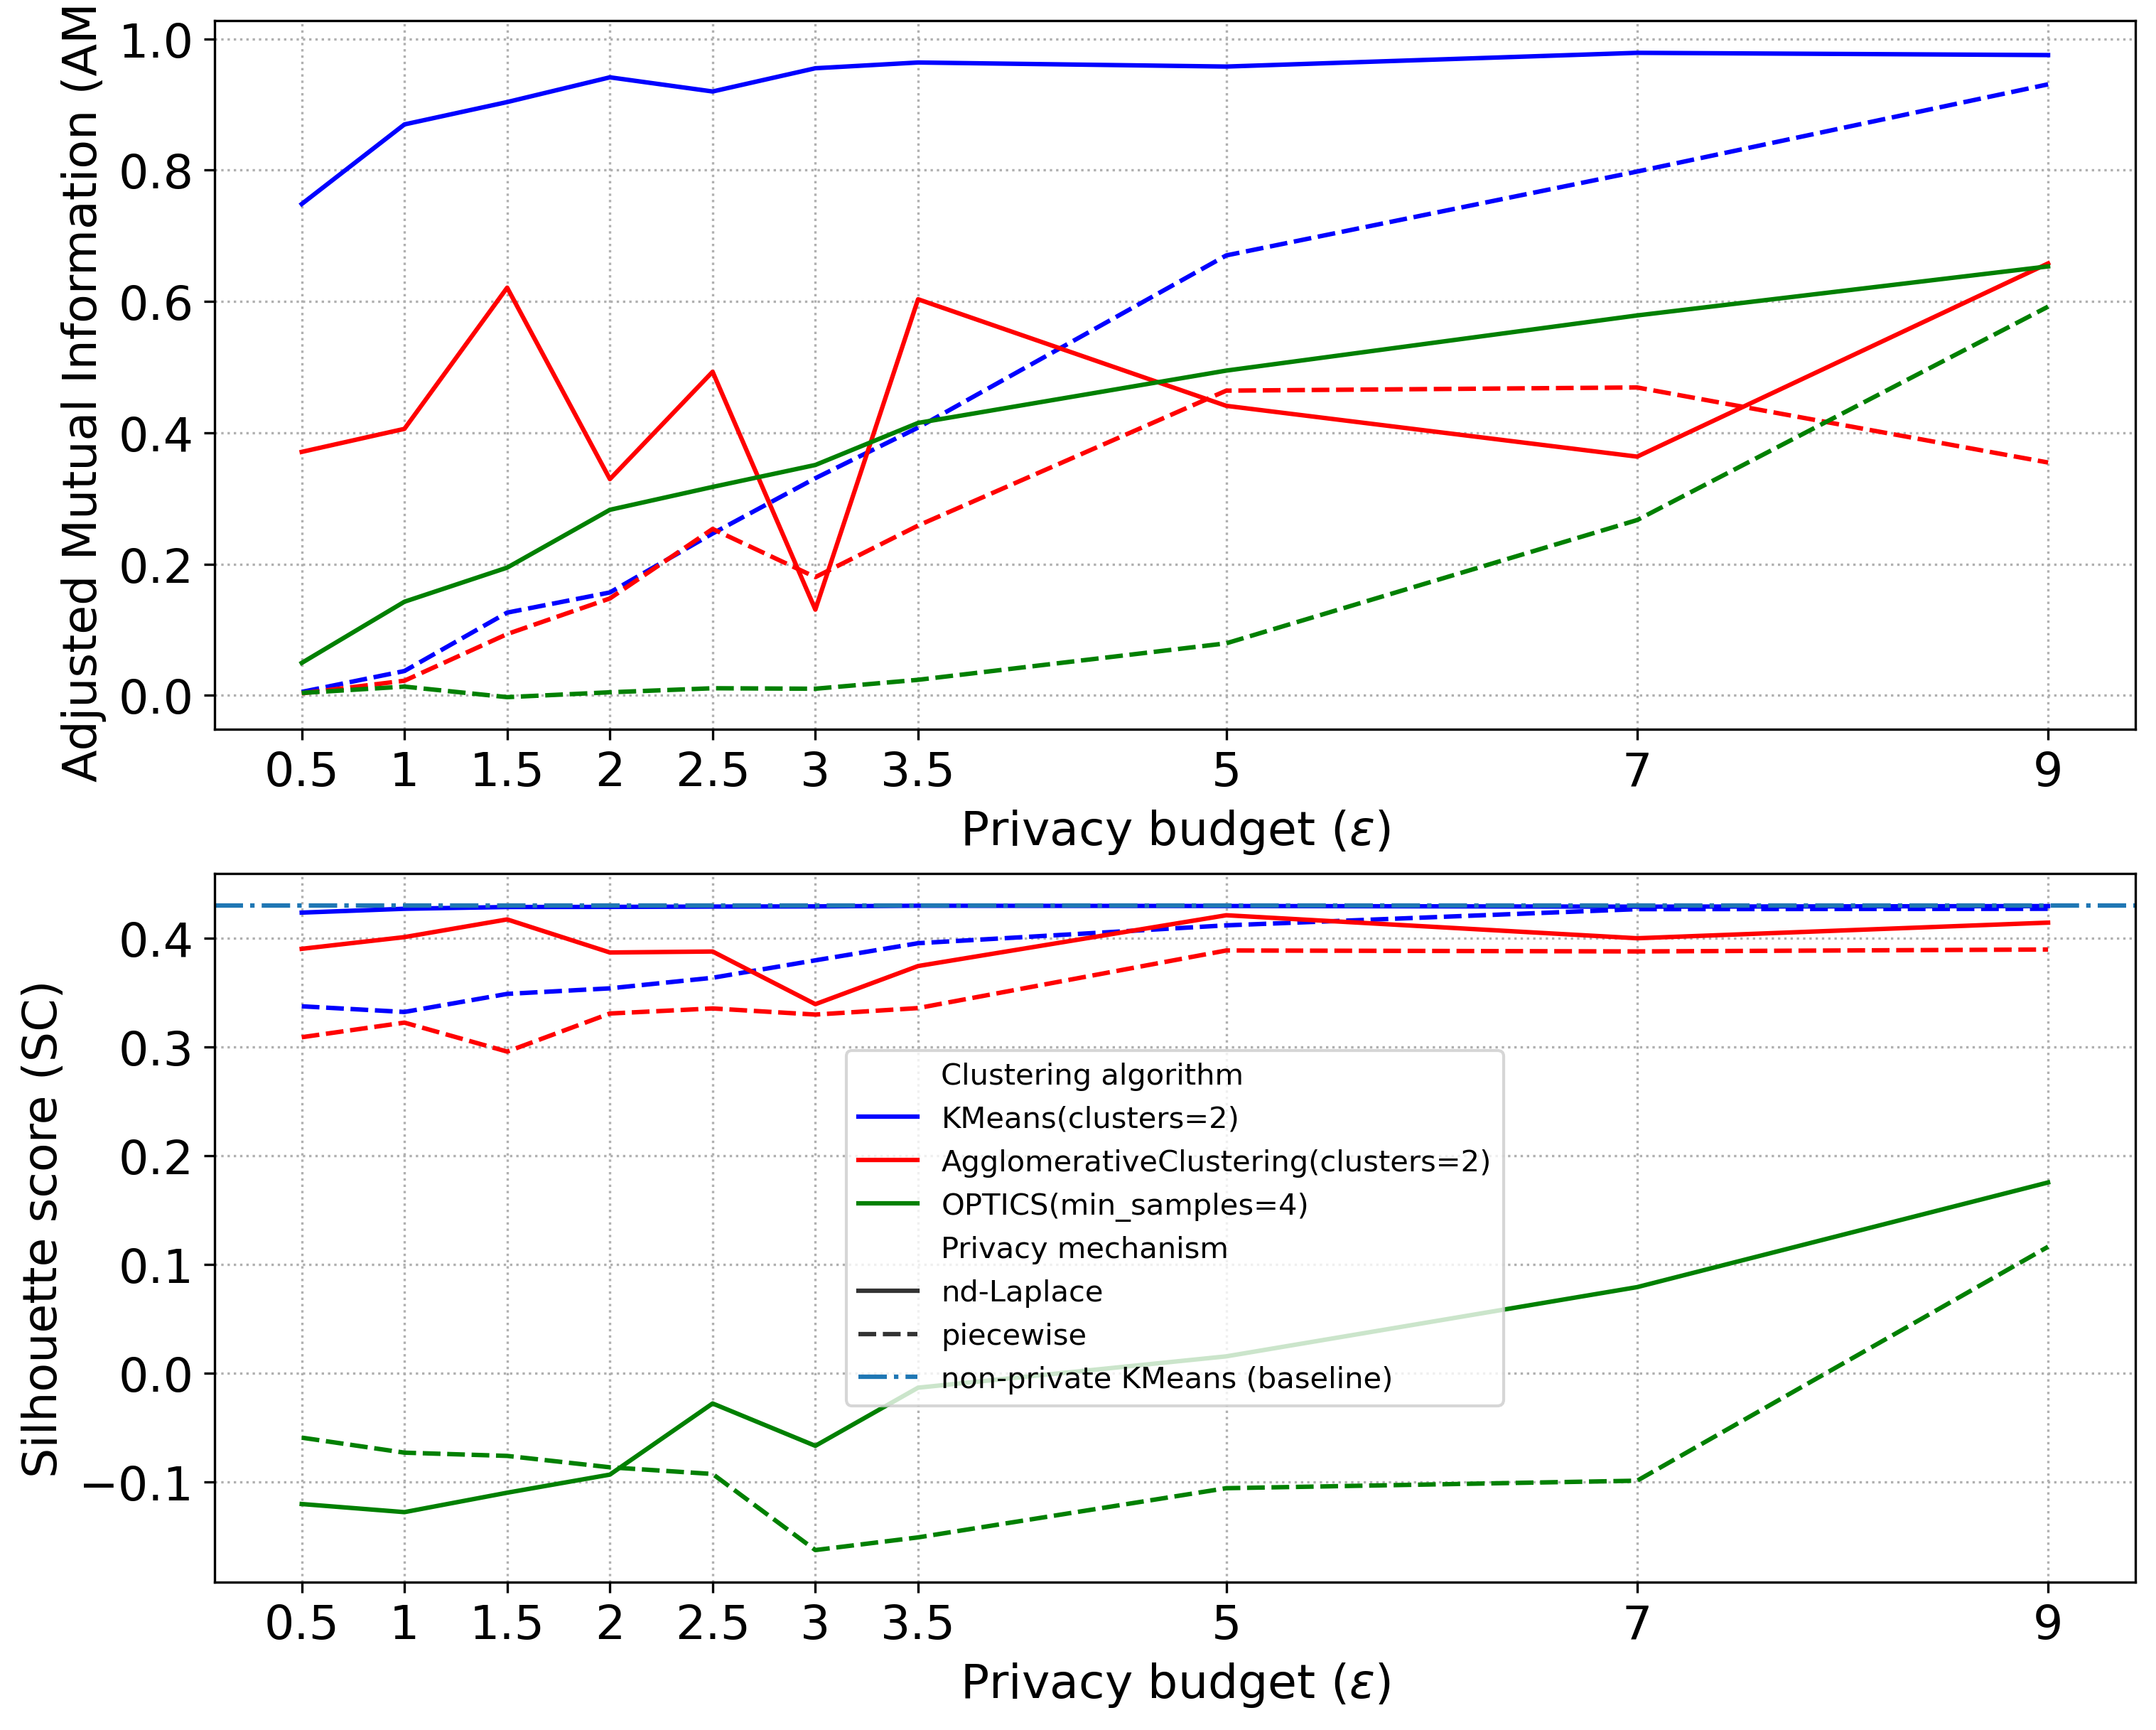
\includegraphics[width=0.9\textwidth]{Results/nd-laplace/nd-Laplace/heart-dataset/ami-and-sc_2_dimensions.png}

  \label{fig:validation-heart-dataset_comparison_2d-laplace}
\end{figure}
Using the K-Means method, the nD-Laplace system works better for all epsilon values. For other methods, the results between the two privacy systems are mostly the same. But, nD-Laplace often does a bit better in \gls{ami} scores. If we compare \gls{optics} with the previous section, we see large improvements. 
When looking at \gls{sc}, both the grouped and K-Means methods do the best for both privacy systems. This is true for most methods. This \gls{ami} score trend matches what we saw with the OPTICS method earlier.

The trends observed in these charts closely mirror those from the seeds-dataset. However, the outcomes here are more consistent. Remarkably, OPTICS stands out in its performance. This can be attributed to the data's configuration. As depicted in Figure \ref{fig:evaluate-optics-seeds-dataset-2d-9eps}, there's a pronounced spread in the nD-Laplace data, similar to the heart-dataset. When data is inherently well-separated, nD-Laplace excels, explaining the strong performance of both Agglomerative and K-Means clustering. This observation is further supported by the \gls{sc}, which aligns closely with the baseline score of K-Means.
\newpage
\begin{figure}[H]
  \centering
  \caption{\textbf{AMI (top) and SC (bottom) for the kD-Laplace mechanism for the 2-dimensional data circle-dataset}}
  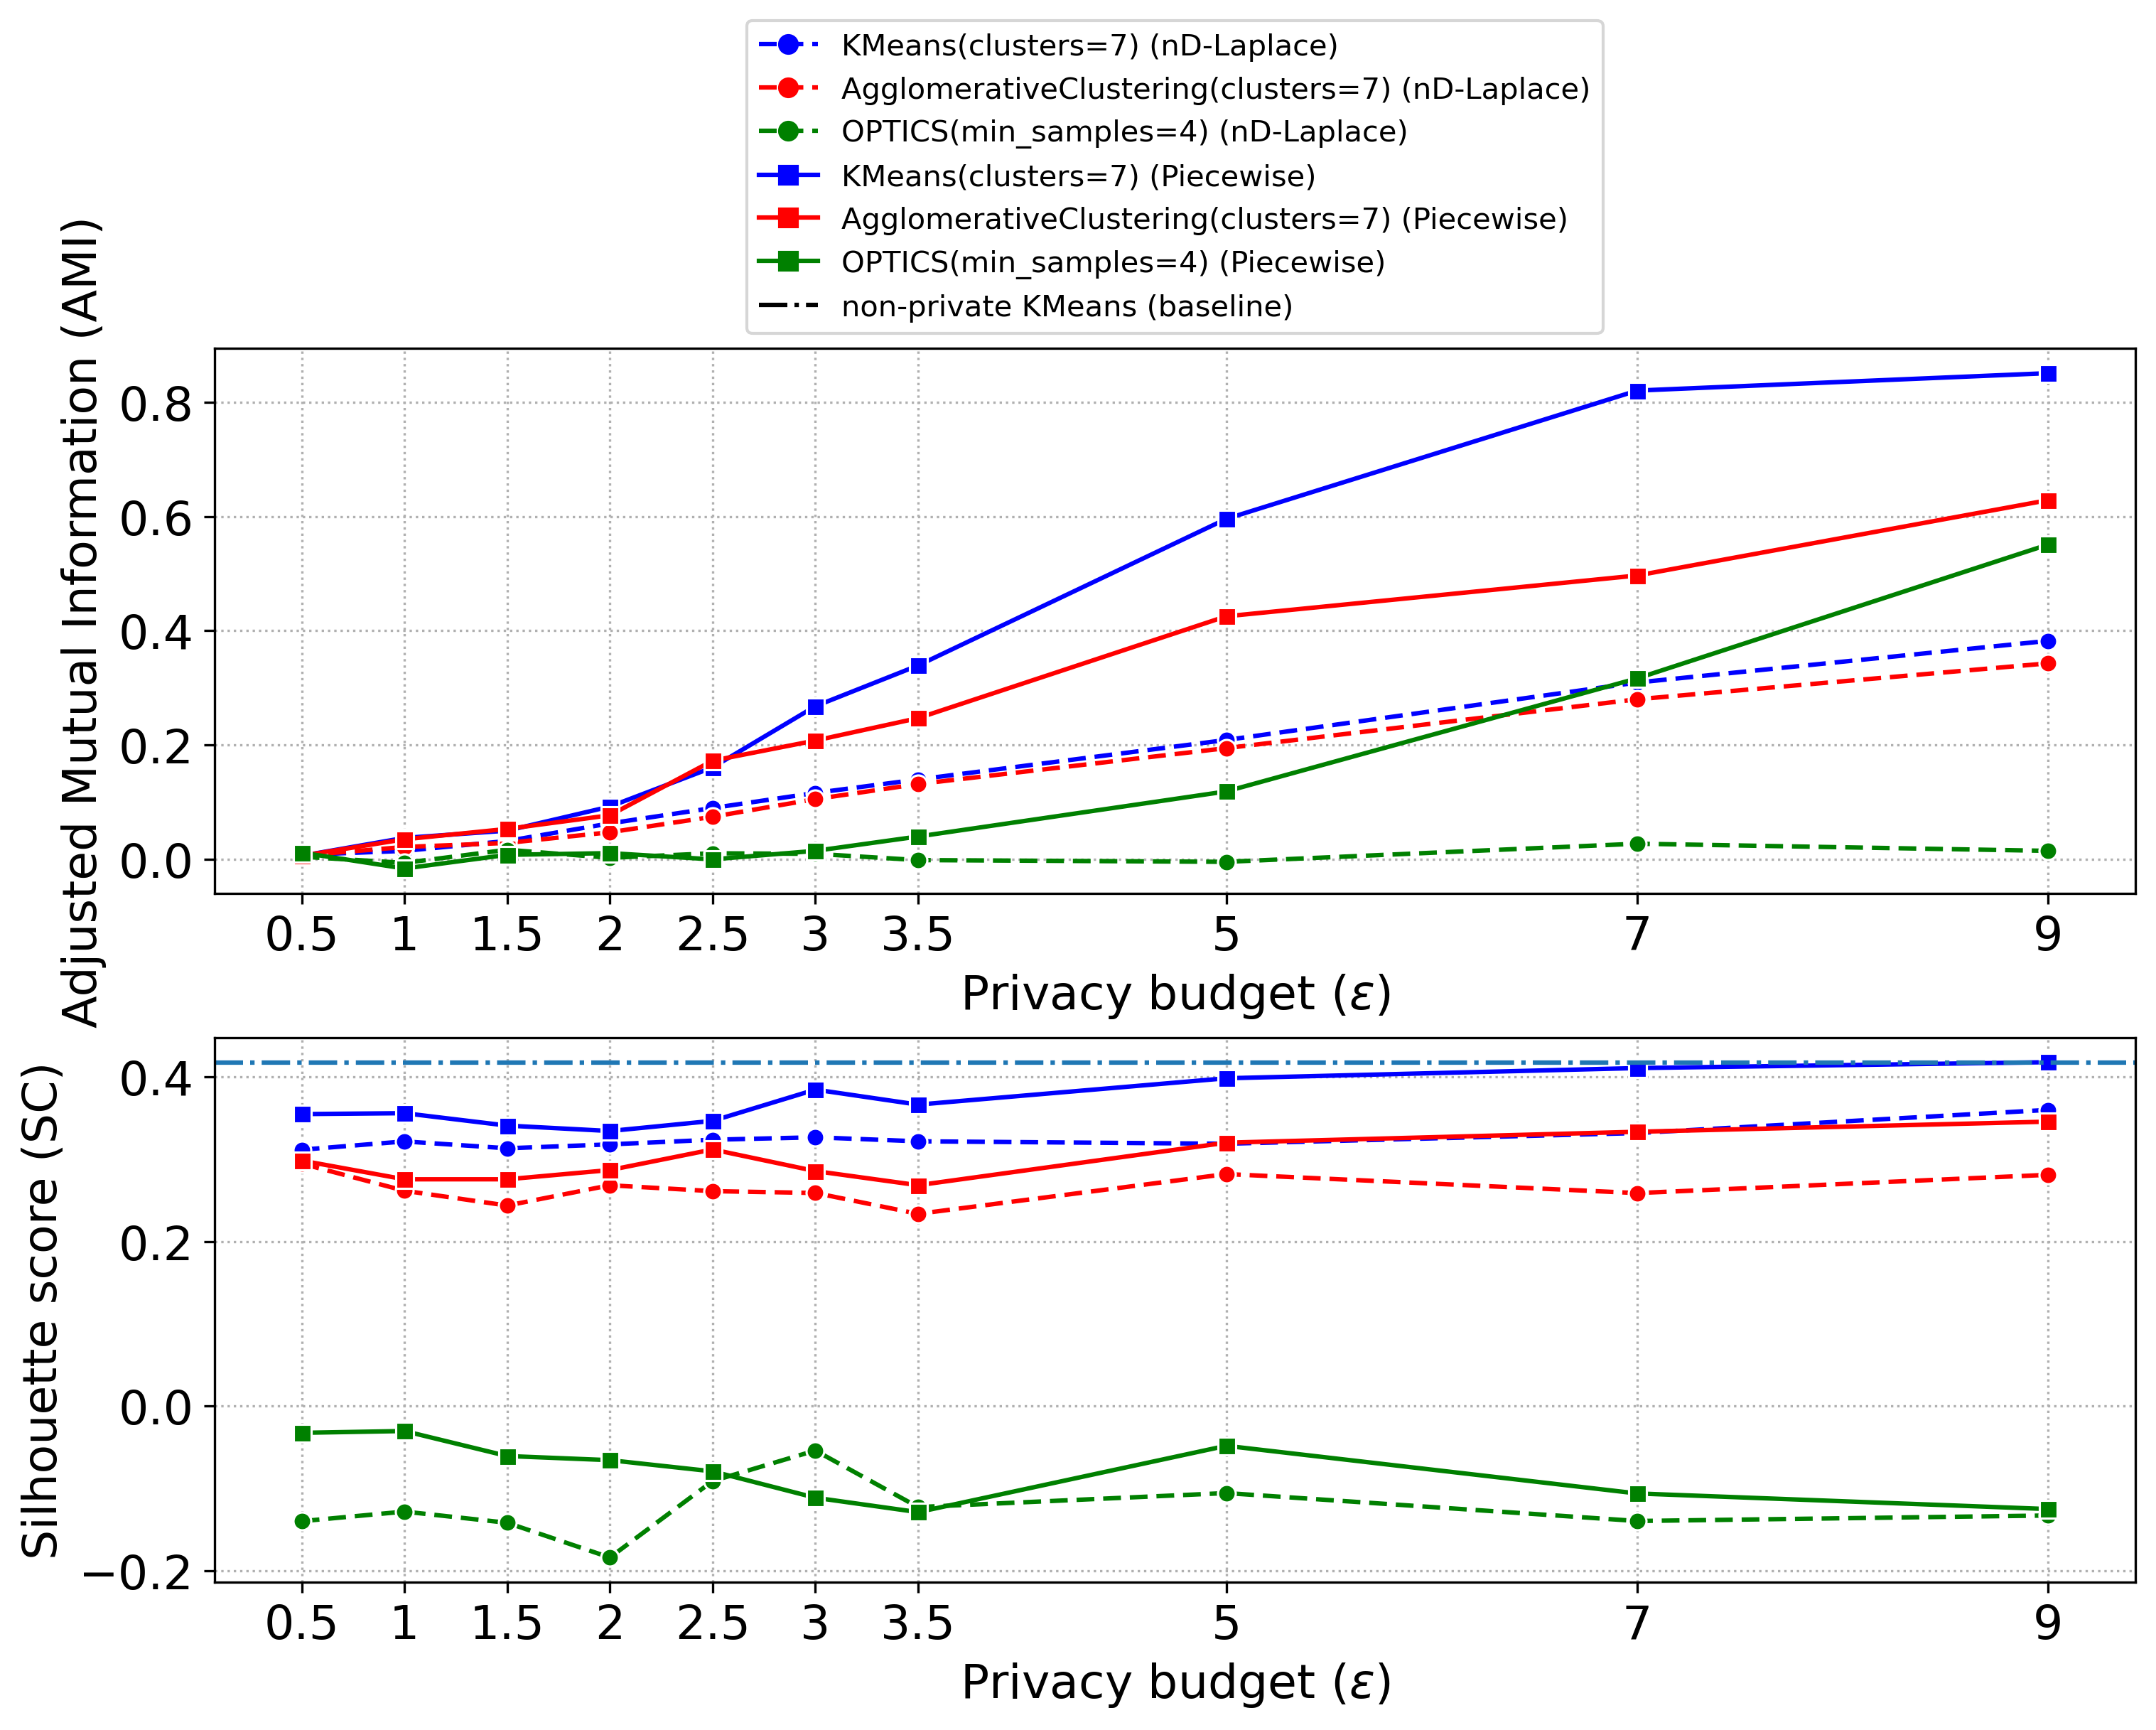
\includegraphics[width=0.9\textwidth]{Results/nd-laplace/nd-Laplace/circle-dataset/ami-and-sc_2_dimensions.png}
  \label{fig:validation-circle-dataset_comparison_2d-laplace}
\end{figure}
Among the two mechanisms, Piecewise consistently achieves the highest scores for all \gls{ami} metrics. Analyzing the three algorithms, a recurring pattern emerges: K-Means leads in performance, trailed by Agglomerative and then \gls{optics}. Notably, within the nD-Laplace mechanism, \gls{optics} significantly lags behind the other algorithms. While a similar trend is observed in the \gls{sc} scores, the disparity between the two mechanisms is less pronounced. Yet, \gls{optics} consistently underperforms across all epsilon values.

We observe the same patterns as with the seeds-dataset; which is shaped as a line.
If there is a thiner line of data, the spread of the data is important. Piecewise mechanism handles this better, to stay close to the original line of data, while nD-Laplace's data is more spread. There are various factors why this issue impacts \gls{optics} the most, but this is probably due to the Euclidean space metric. Here, the distance matters more then similar metrics, and 
\newpage
\begin{figure}[H]
  \centering
  \caption{\textbf{AMI (top) and SC (bottom) for the kD-Laplace and Piecewise mechanisms for the 2-dimensional data line-dataset}}
  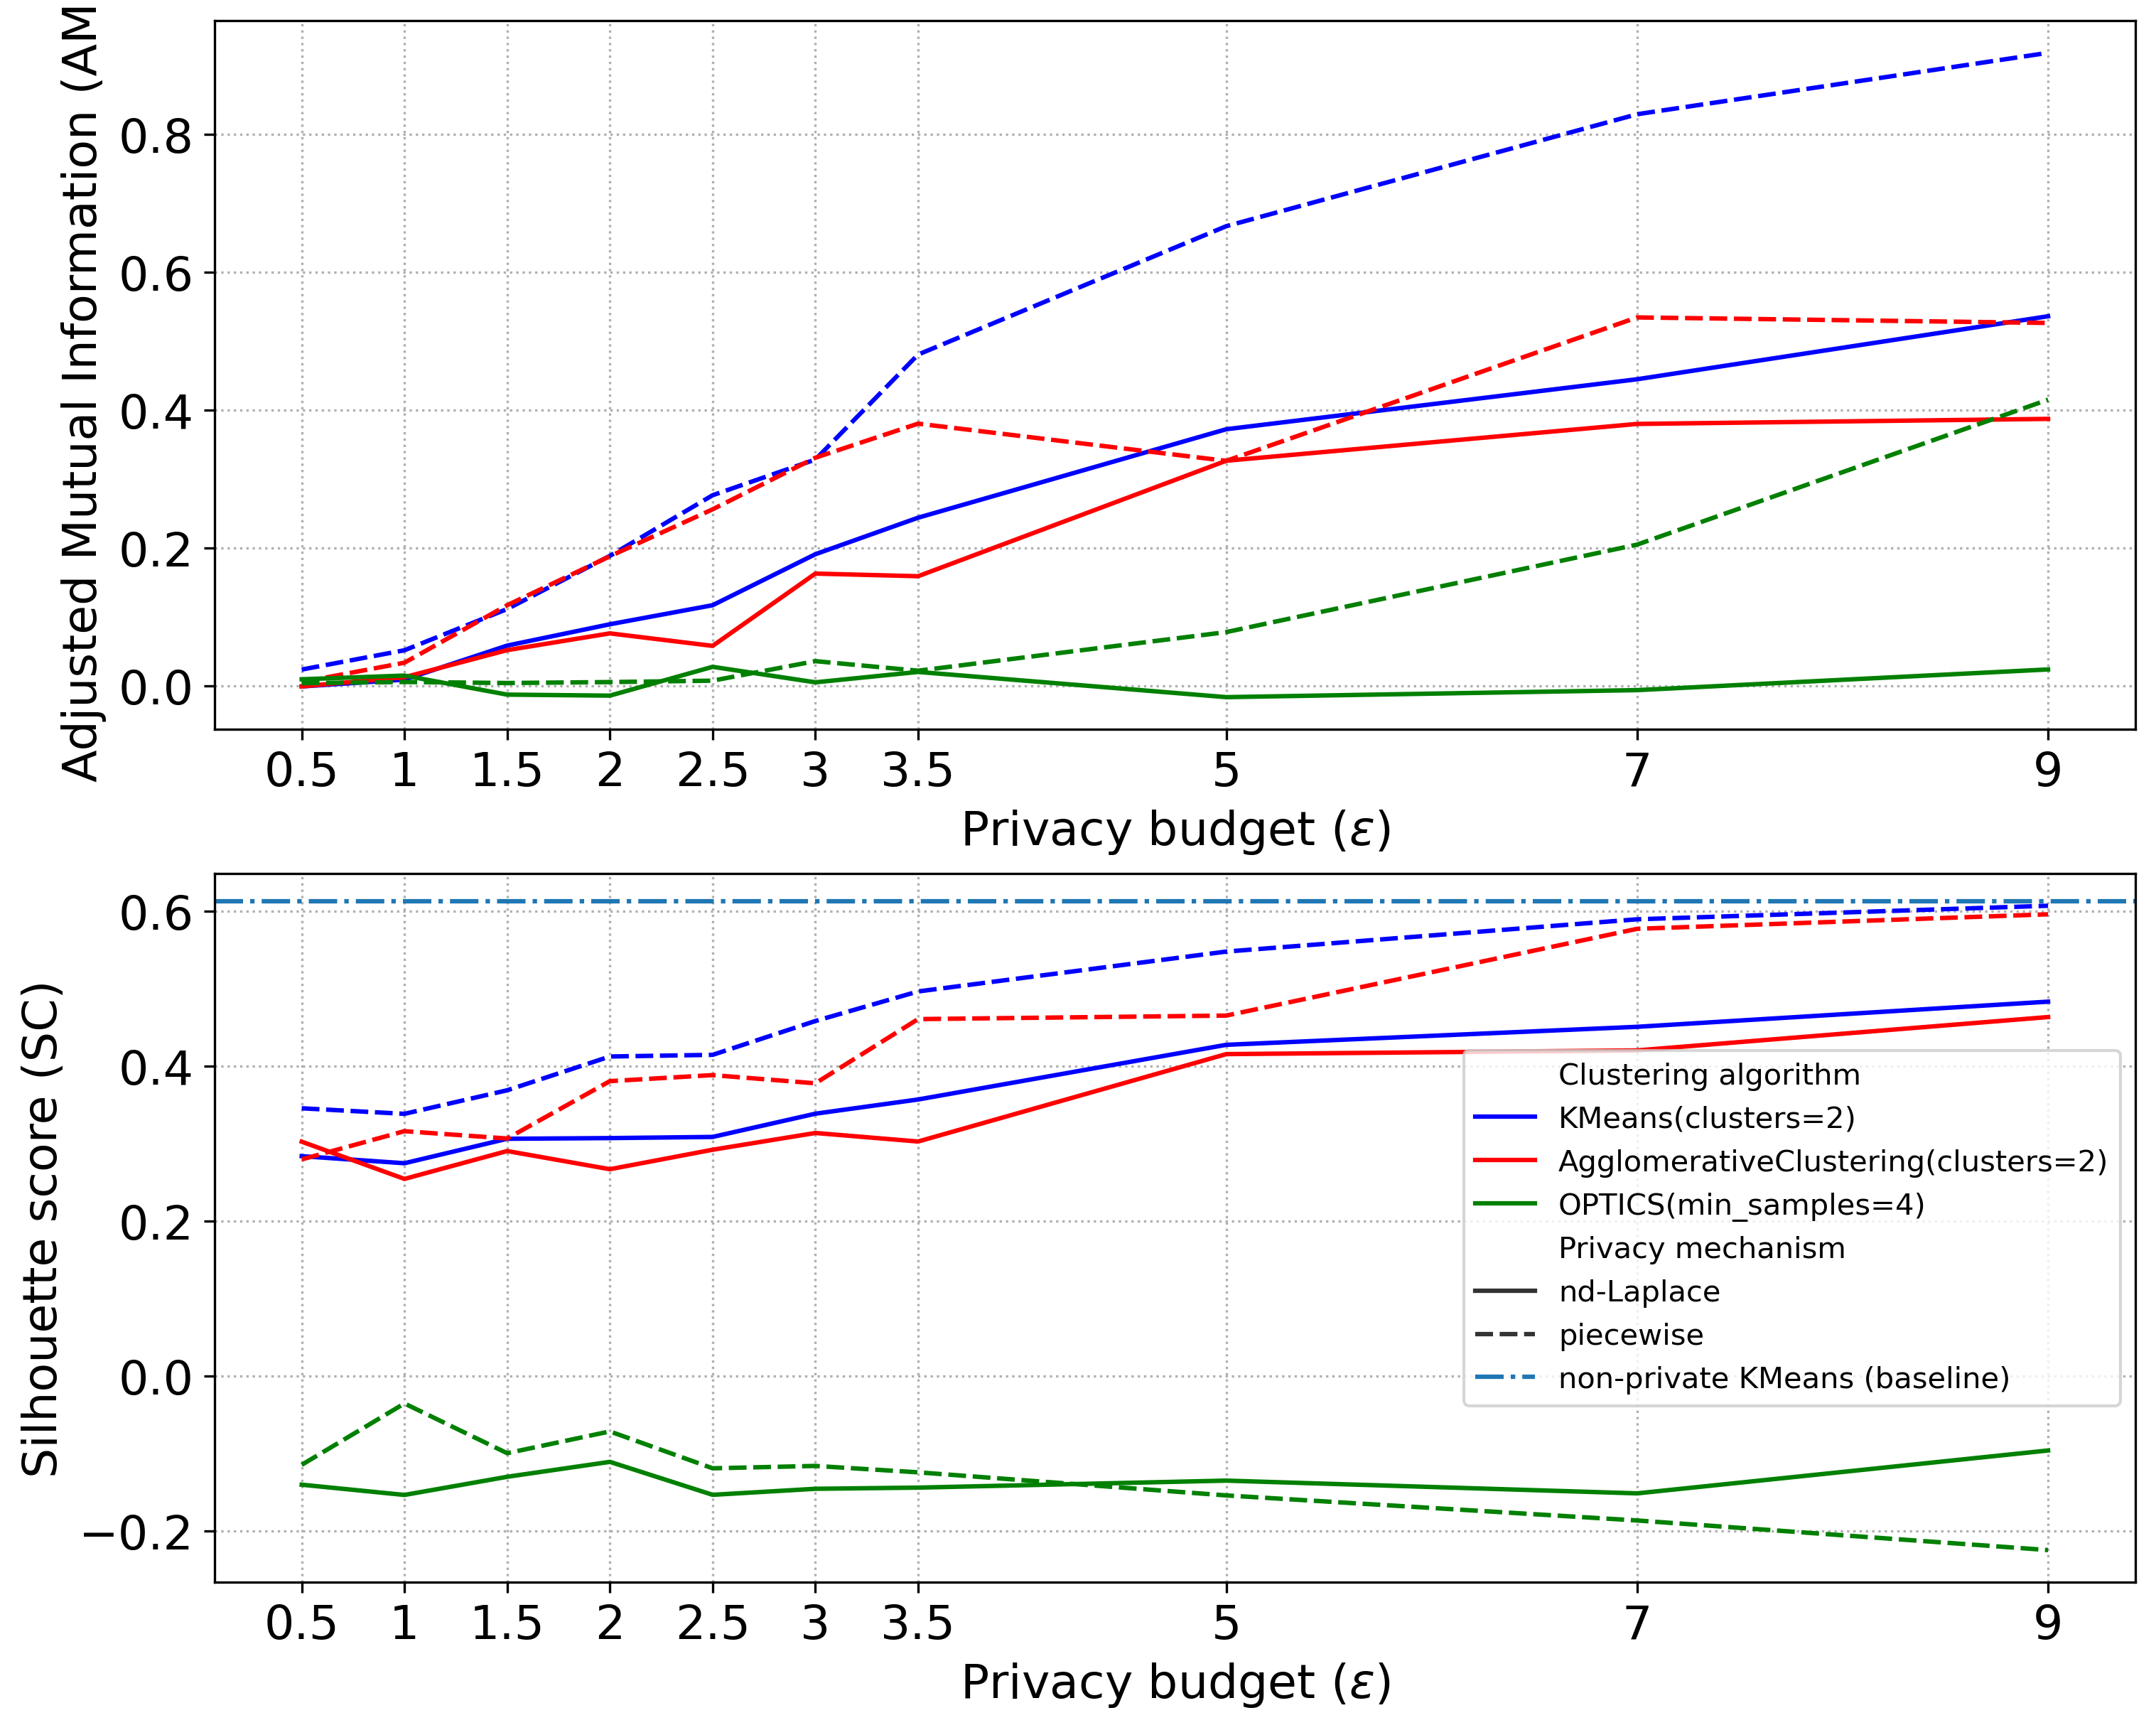
\includegraphics[width=0.9\textwidth]{Results/nd-laplace/nd-Laplace/line-dataset/ami-and-sc_2_dimensions.png}
  \label{fig:validation-line-dataset_comparison_2d-laplace}
\end{figure}
The nD-Laplace algorithm performs best with a privacy budget of 9 for K-Means (\gls{ami} 0.55 - 0.6).
\gls{ag} performs slightly worse with a budget of 9 (\gls{ami} 0.4).
Piecewise outperforms other methods, scoring 0.83 \gls{ami} for K-Means at budget 9 and better for different budgets, .
For \gls{sc}, the mechanisms have similar scores, with Piecewise at baseline from budget 5, kD-Laplace at 7, and \gls{ag} beyond baseline from budget 9. 

Overall, the trends observed with the heart-dataset are not mirrored here. The Piecewise mechanism consistently outperforms nD-Laplace across nearly all privacy budgets. Given that the shapes of the line-dataset and seeds-dataset are expected to be analogous, we further illustrate this with the subsequent plot:

\begin{figure}[H]
\centering
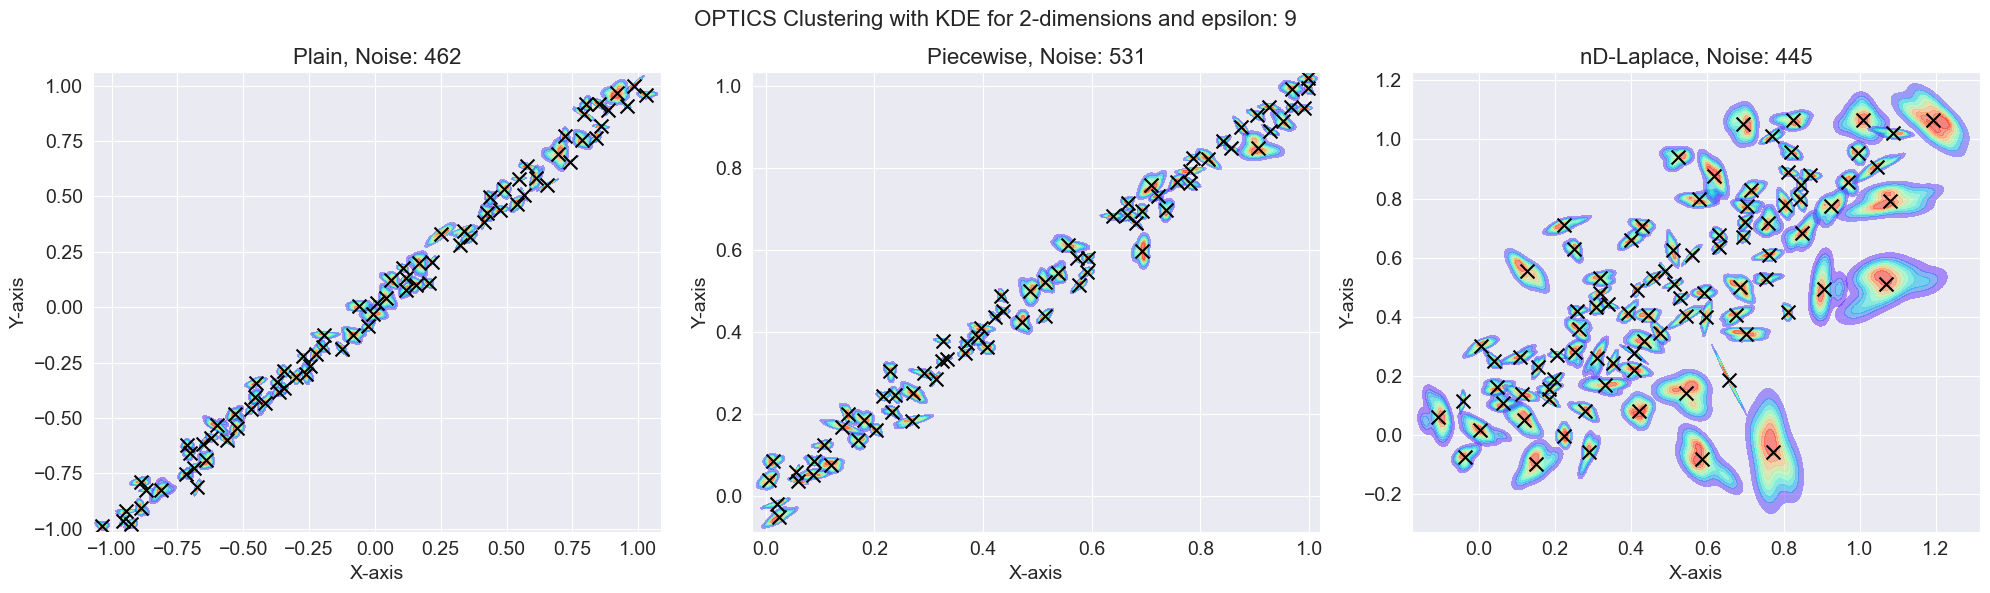
\includegraphics[width=1\linewidth]{Discussion/behaviour-2d-line-dataset&optics.png}
\caption{Evaluating OPTICS and density of points for 2-dimensional Line dataset with epsilon 9}
\label{fig:validation-Line-dataset_comparison_2d-laplace}
\end{figure}

The plot above displays the \gls{optics} scores, denoted by black markers. Even though the data bears resemblance to the seeds-dataset, the dispersion is significantly greater for the nD-Laplace mechanism. This can be attributed to the line shape of the data, as the nD-Laplace mechanism disperses noise uniformly in all directions. However, the extent of this dispersion is notably greater than that observed in the seeds-dataset, leading to inferior results.
\todo[inline]{Analyze why this is such a big difference}

\newpage
\begin{figure}[H]
  \centering
  \caption{\textbf{AMI (top) and SC (bottom) for the kD-Laplace and Piecewise mechanisms for the 2-dimensional data skewed-dataset}}
  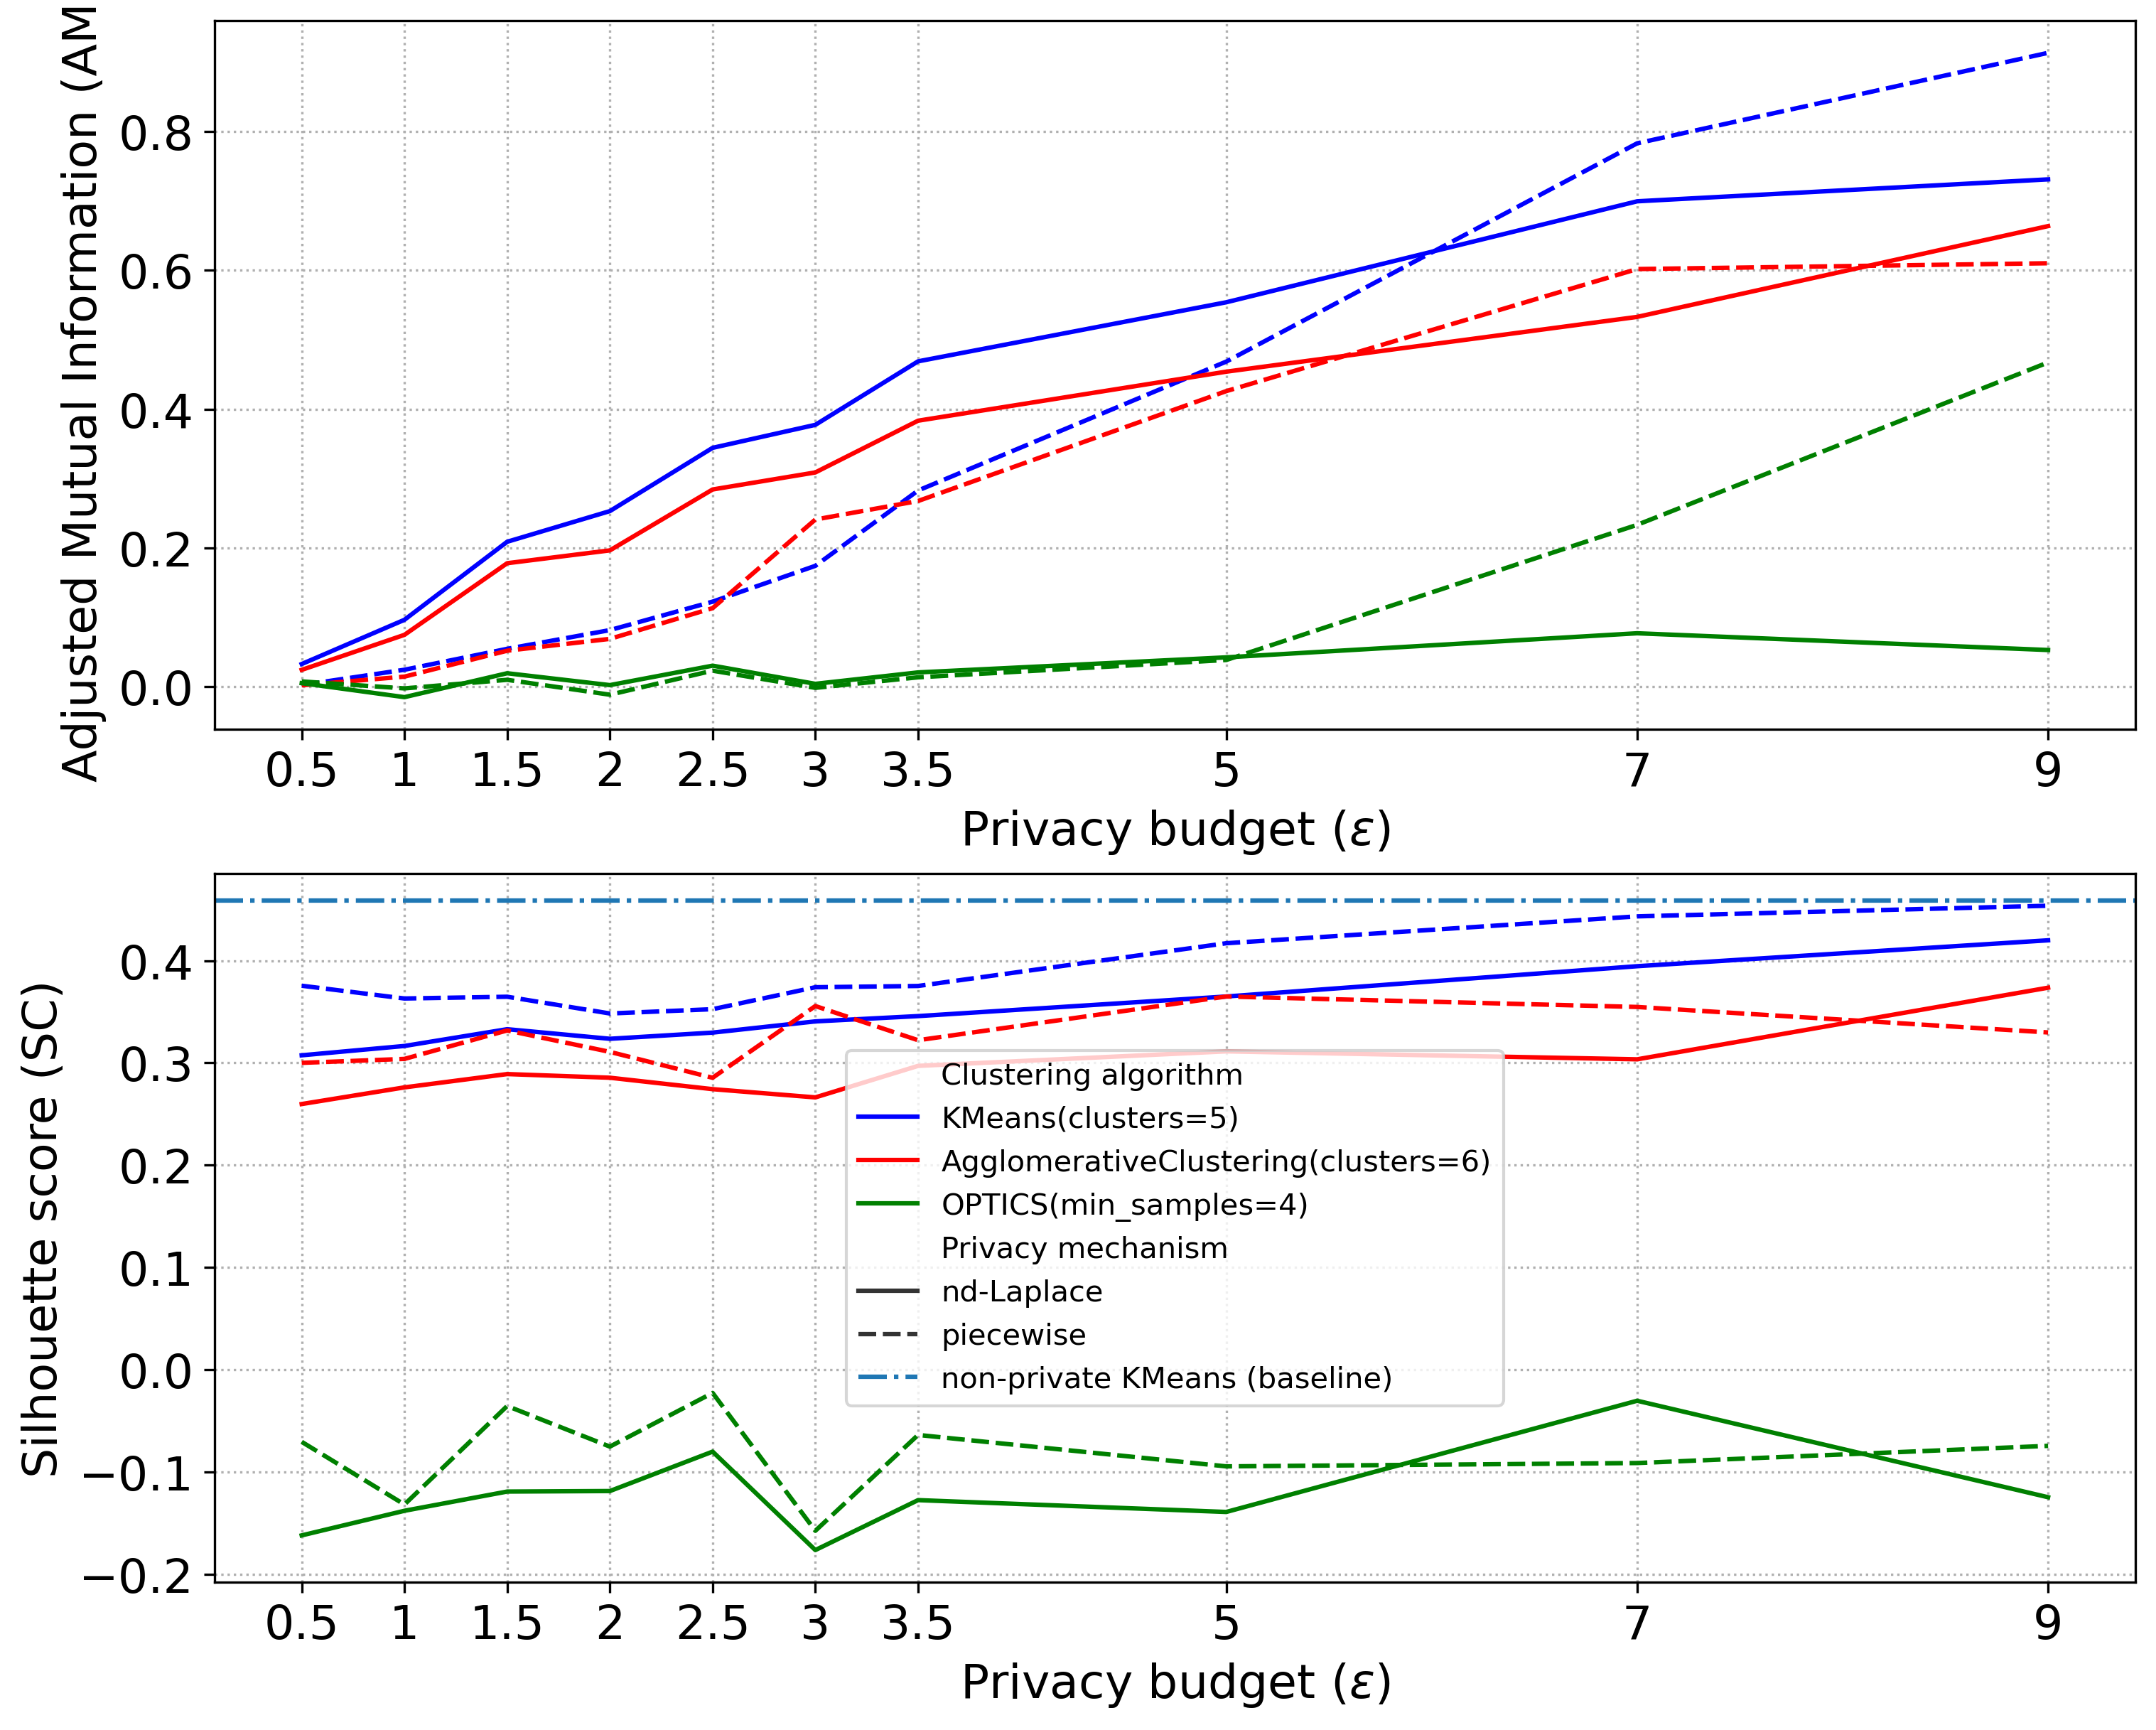
\includegraphics[width=0.9\textwidth]{Results/nd-laplace/nd-Laplace/skewed-dataset/ami-and-sc_2_dimensions.png}
  \label{fig:validation-skewed-dataset_comparison_2d-laplace}
\end{figure}
In our analysis, the nD-Laplace mechanism exhibits its peak performance when paired with K-Means, achieving an \gls{ami} range of 0.74 to 0.78 at privacy budgets of 7 and 9. Conversely, while Piecewise registers higher scores with K-Means for these specific budgets, it lags behind nD-Laplace for other privacy budgets. When considering the \gls{ag} scores, both mechanisms present comparable results. However, nD-Laplace has a slight edge, particularly at lower privacy budgets. This trend of nD-Laplace's superiority at reduced privacy budgets is consistent across different algorithms. A recurring observation is the under performance of \gls{optics}, although it still manages to score 0.43 at a privacy budget of 9 when using the Piecewise mechanism. As for the \gls{sc} metric, the patterns remain consistent: K-Means emerges as the top performer for both mechanisms, while \gls{optics} records notably low scores, even dipping below 0.0 for both mechanisms.

\newpage
\subsection{3-dimensional data}
\begin{figure}[H]
  \centering
  \caption{\textbf{AMI (top) and SC (bottom) for the kD-Laplace and Piecewse mechanisms for the 3-dimensional data seeds-dataset}}
  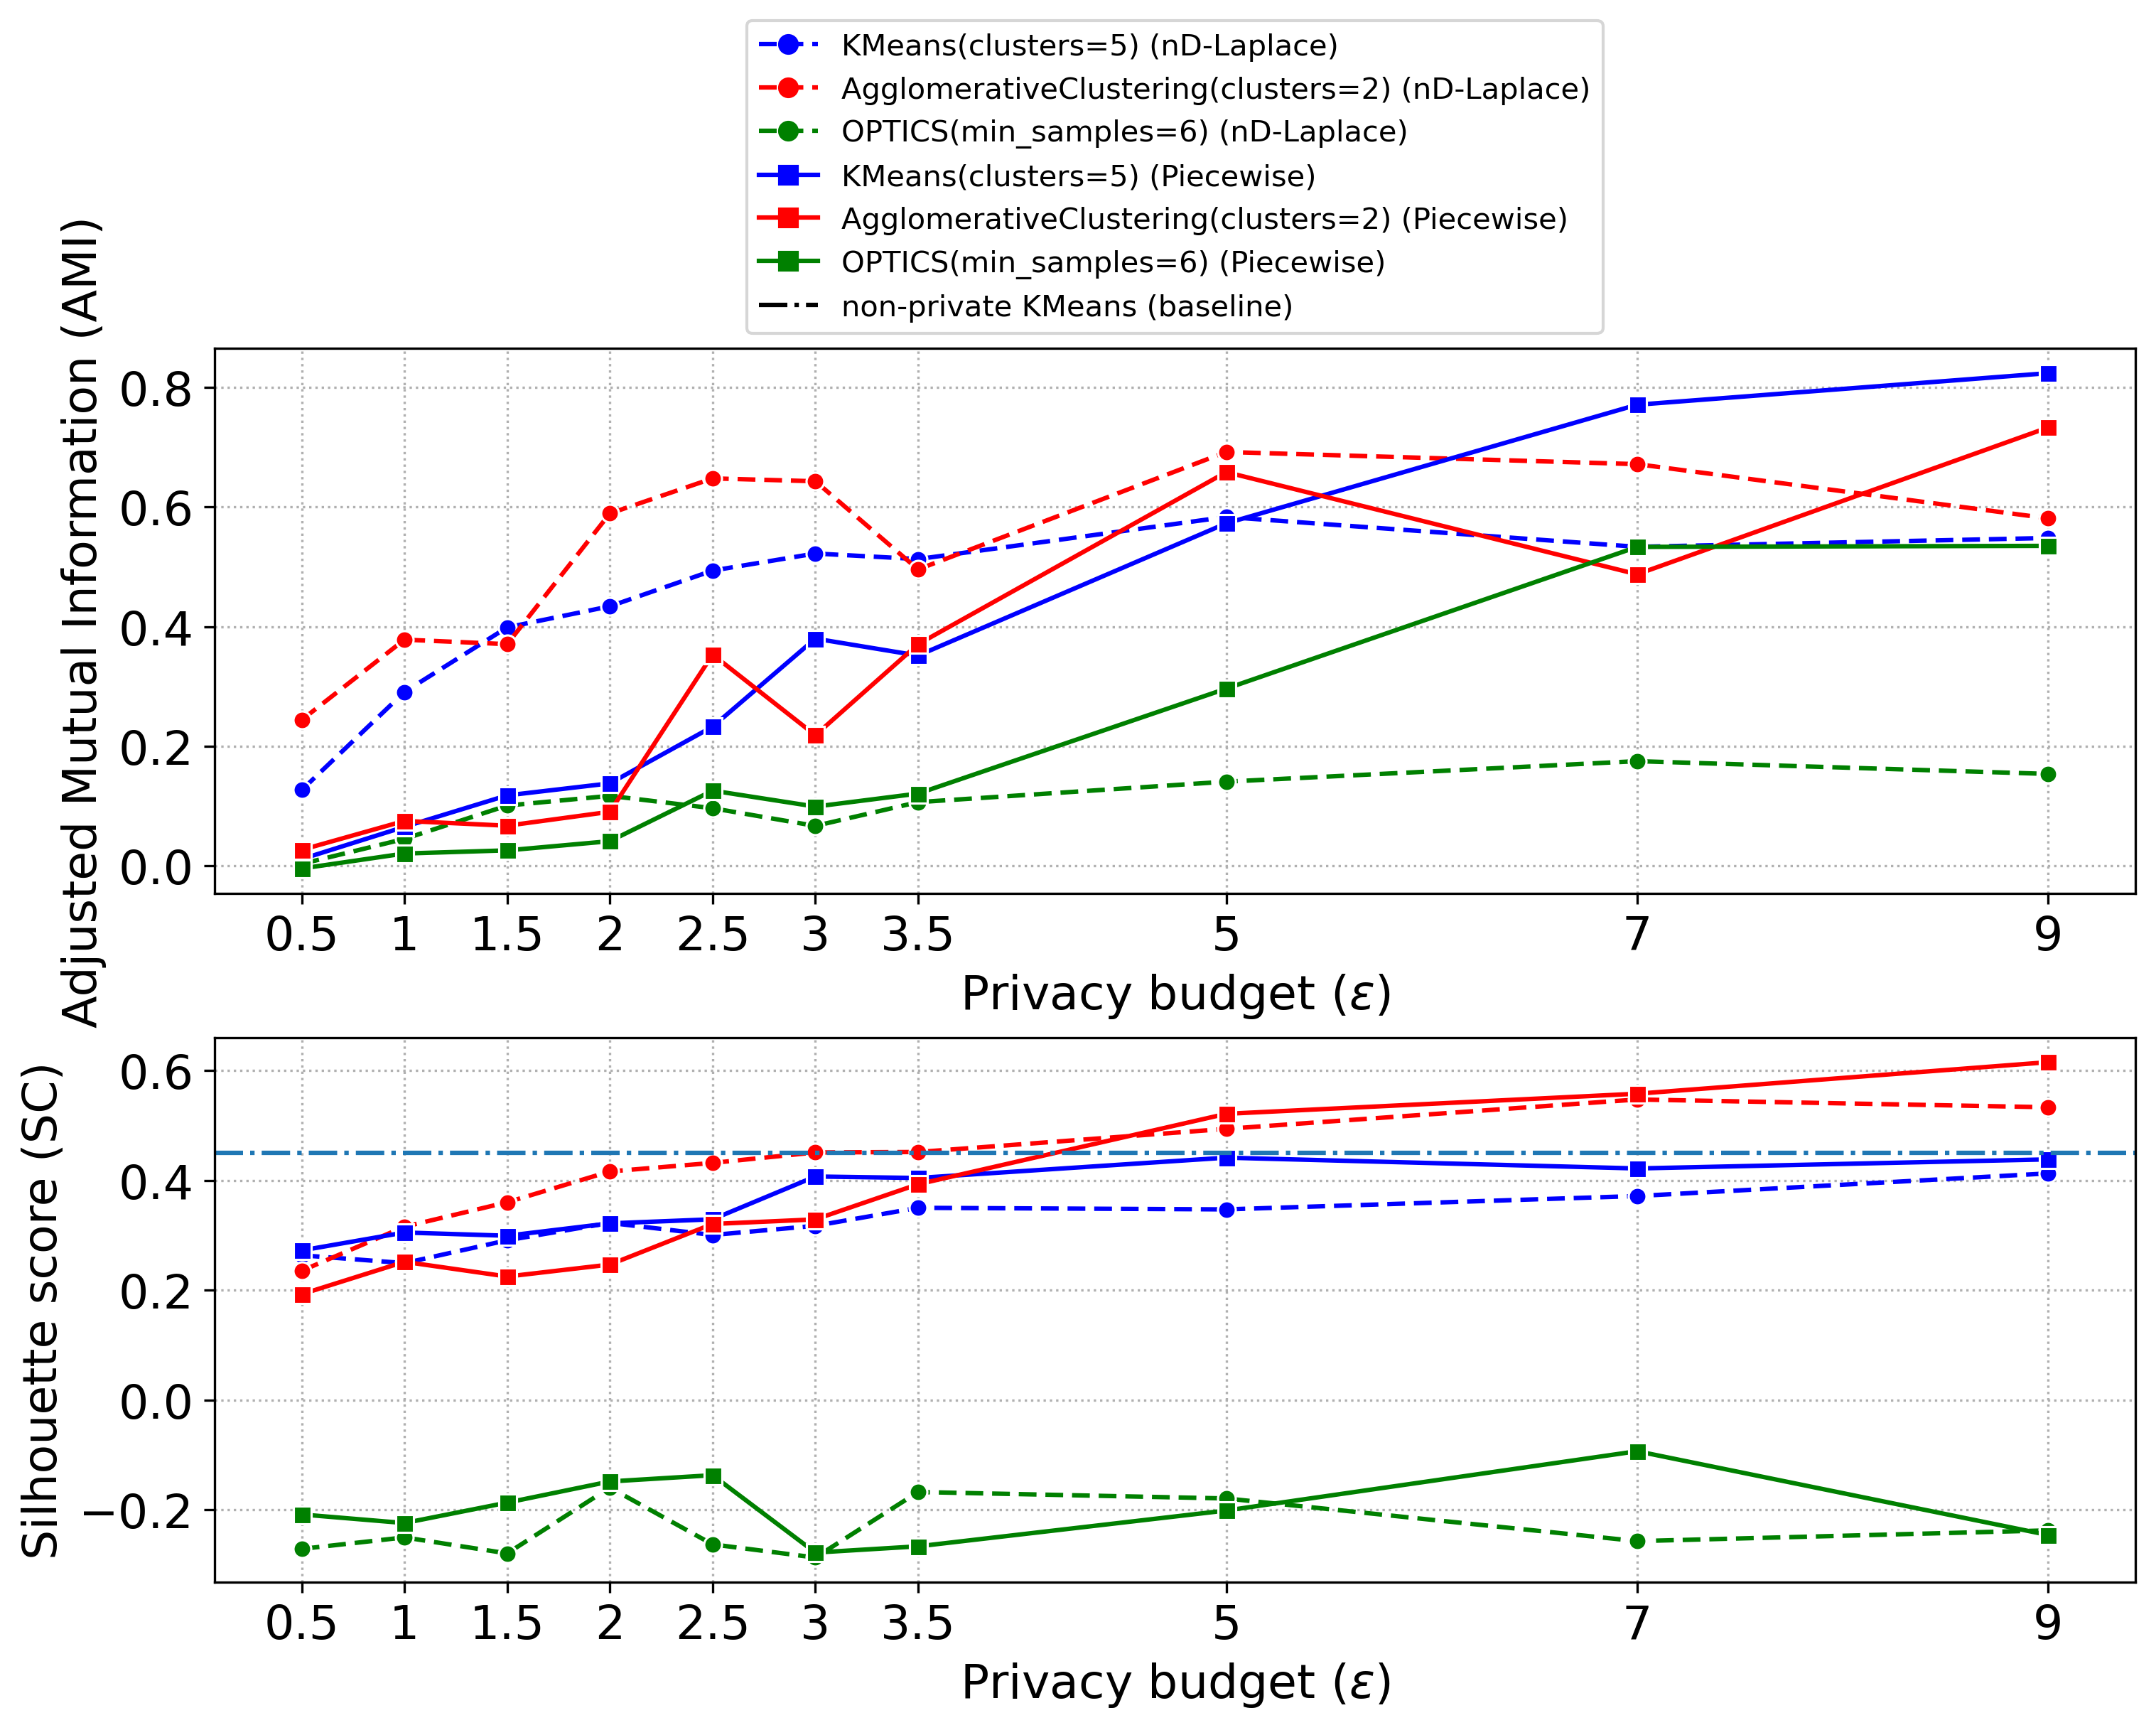
\includegraphics[width=0.9\textwidth]{Results/nd-laplace/nd-Laplace/seeds-dataset/ami-and-sc_3_dimensions.png}
  \label{fig:validation-seeds-dataset_comparison_3d-laplace}
\end{figure}
For the 3-dimensional data, the trend mirrors that observed in the 2-dimensional version of the seeds-dataset. In the range from 0.5 to 5, nD-Laplace outperforms both \gls{ag} and K-Means. Beyond this range, the Piecewise mechanism registers scores approximately 0.10 - 0.20 points higher than nD-Laplace. Conversely, nD-Laplace consistently scores higher for \gls{ag}, with the exception of epsilon 9. Notably, \gls{optics} yields a low score (less than 0.2 \gls{ami}) with nD-Laplace, whereas with Piecewise, the scores range between 0.2 and 0.58 for a privacy budget of 3.5.

For the \gls{sc} metric, the trend is consistent with the \gls{ami} score. However, \gls{ag} achieves a score surpassing the baseline for privacy budgets ranging from 3.5 to 9 across both mechanisms.

In other visual representations, both \gls{ami} and \gls{sc} metrics exhibit comparable trends. Yet, in this specific plot, \gls{ag} is superior to K-Means in performance. While the cluster quality is elevated, it doesn't translate to a higher \gls{ag} score. This suggests that while the mechanisms maintain clusters, they don't necessarily preserve the exact cluster configurations or sizes as observed with the non-private K-Means.

\newpage
\begin{figure}[H]
  \centering

  \caption{\textbf{AMI (top) and SC (bottom) for the kD-Laplace and Piecewise mechanisms for the 3-dimensional data heart-dataset}}
  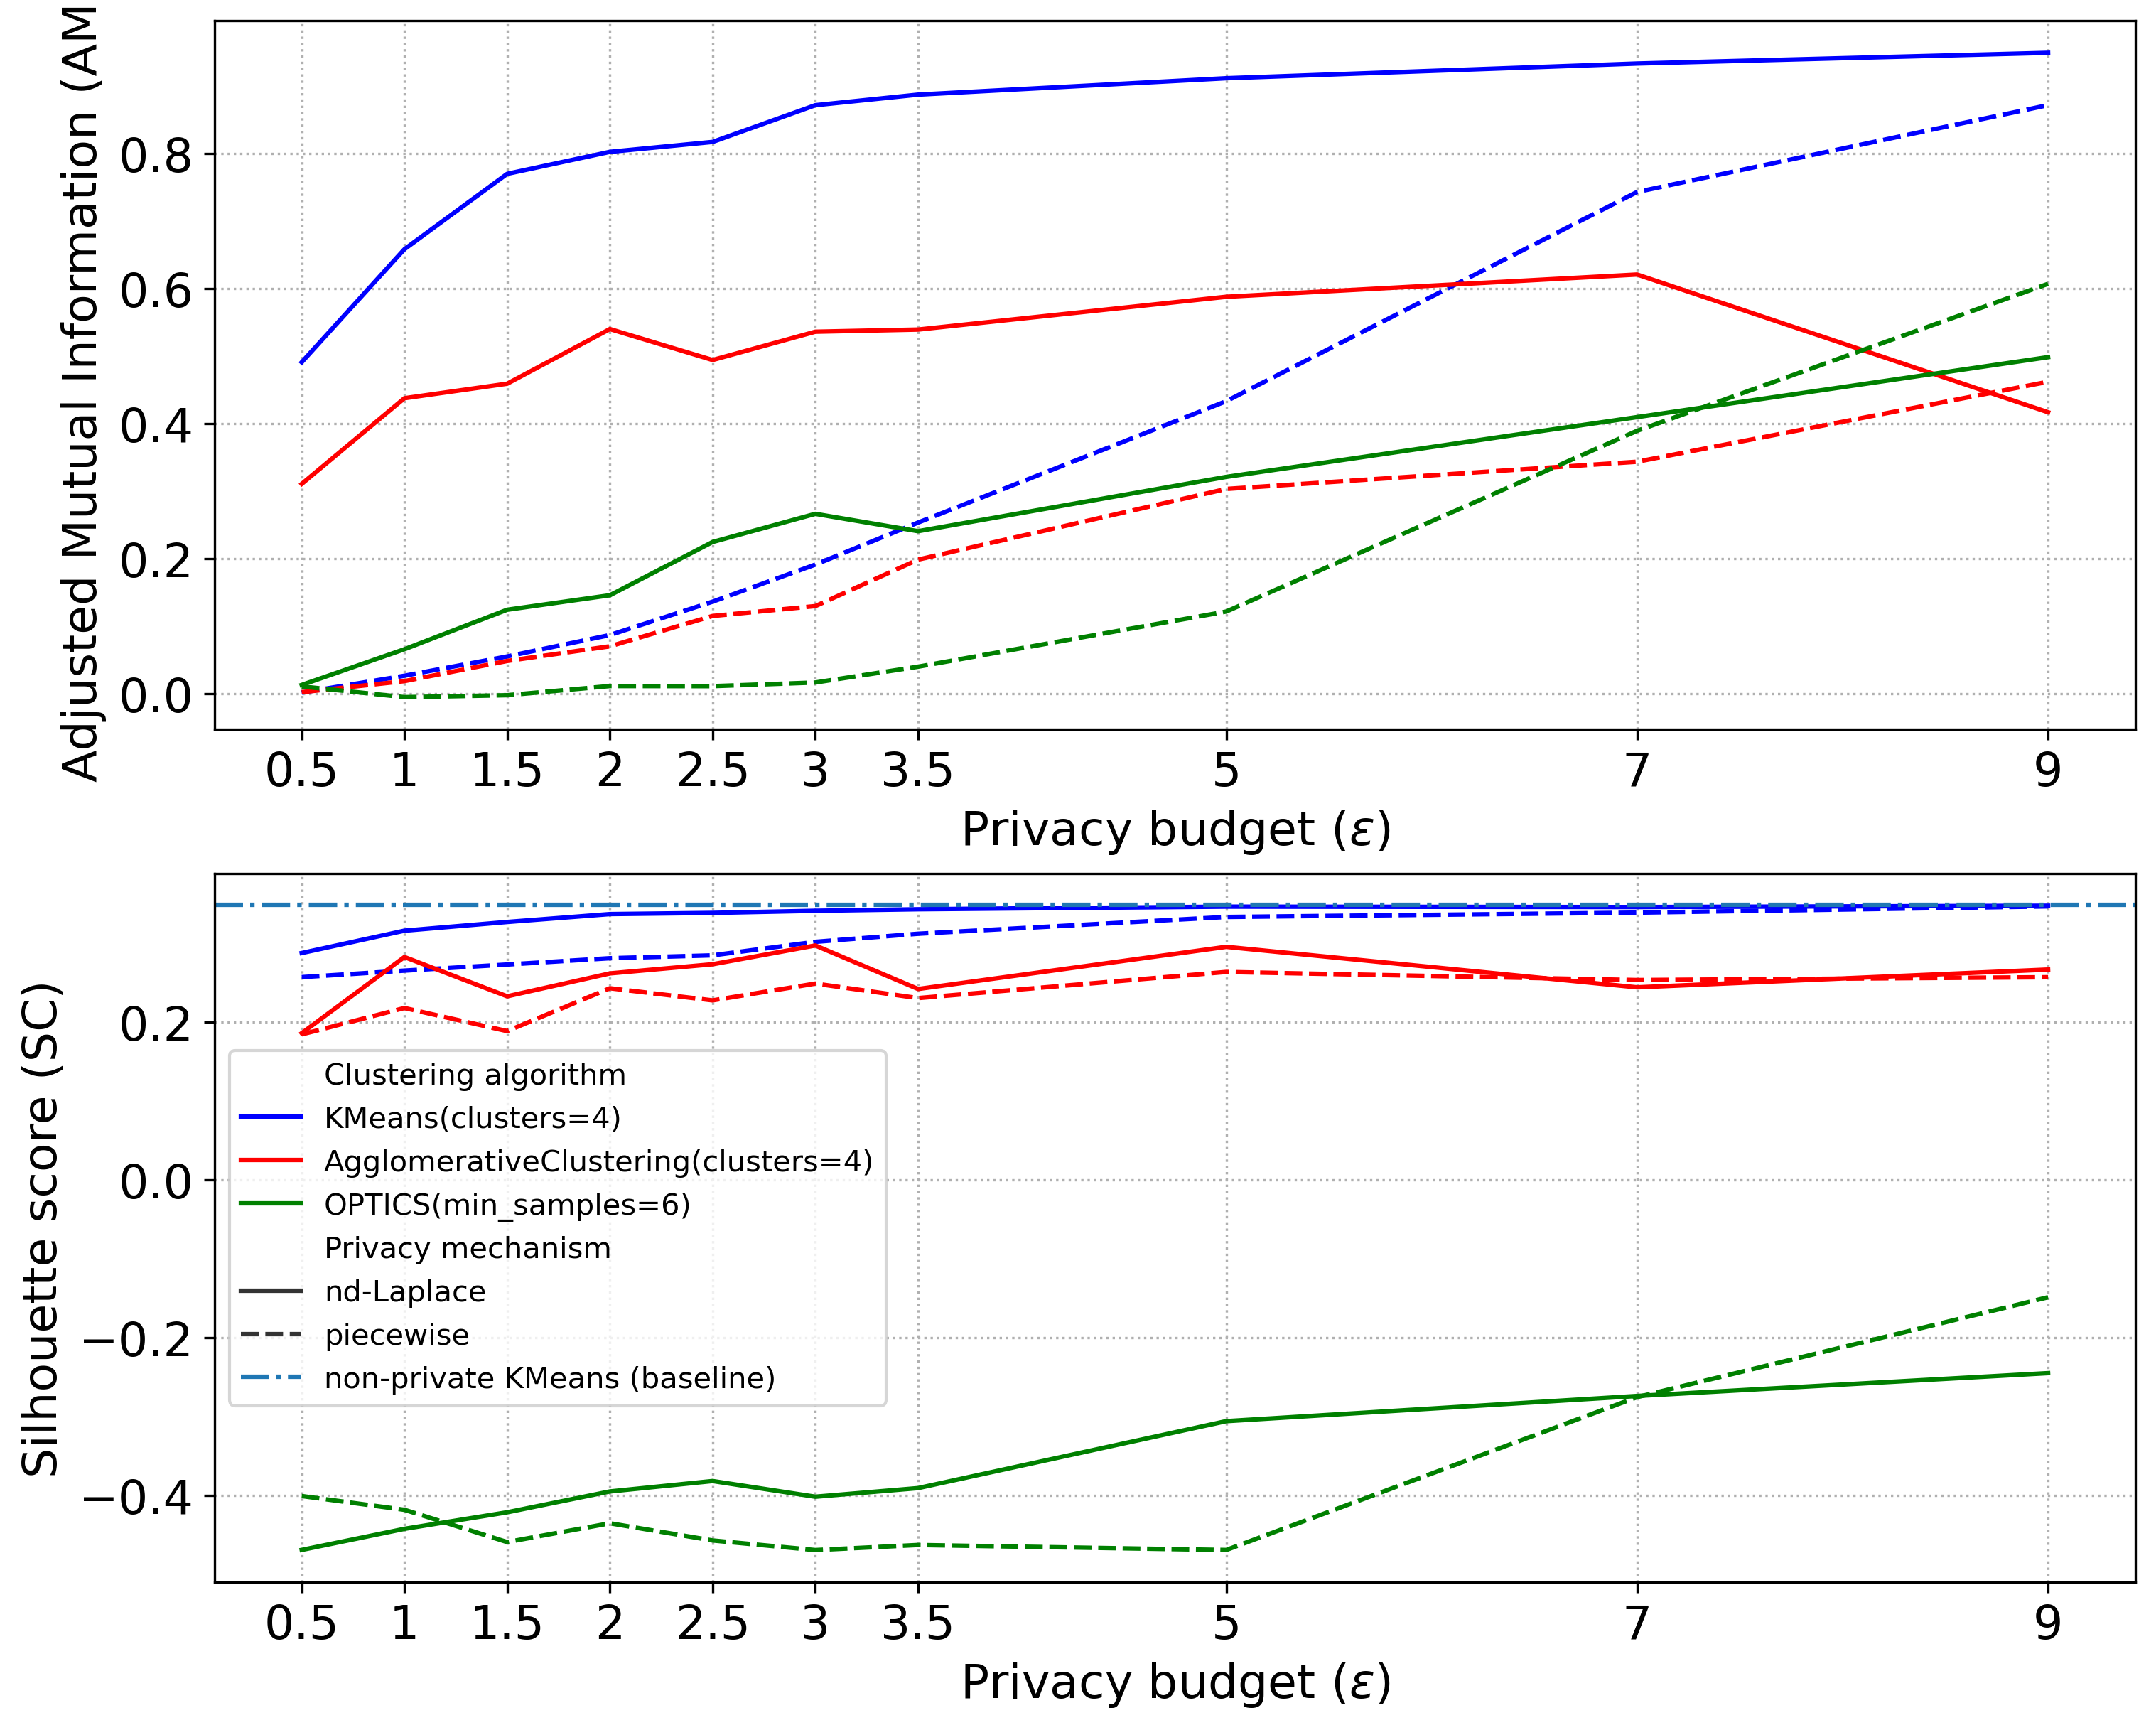
\includegraphics[width=0.9\textwidth]{Results/nd-laplace/nd-Laplace/heart-dataset/ami-and-sc_3_dimensions.png}
  \label{fig:validation-heart-dataset_comparison_3d-laplace}
\end{figure}
The nD-Laplace method gets good results, scoring around +/- 0.87 \gls{ami} for K-Means when the budgets are 7 and 9. This is similar to what we saw with the simpler 2D heart-dataset using the same method. We also noticed that \gls{optics} scores got better compared to other datasets, which matches the results from the 2D heart-dataset. However, \gls{ag} scores a bit lower than K-Means, but the overall pattern is similar.

For the Piecewise method, the scores are below 0.6 \gls{ami} when the budgets are less than 7, but it goes up to 0.8 \gls{ami} for K-Means. When we look at \gls{sc}, both Piecewise and nD-Laplace meet the standard scores for \gls{ag} and K-Means.

Even though \gls{optics} gets high scores for \gls{ami}, it doesn't do as well for \gls{sc}. The main job of \gls{ami} is to compare \gls{optics} to the non-private variant. But if \gls{sc} is low and \gls{ami} is high, it shows that also the non-private has incorrect clusterings.
\newpage
\begin{figure}[H]
  \centering

  \caption{\textbf{AMI (top) and SC (bottom) for the kD-Laplace and Piecewise mechanisms for the 3-dimensional data circle-dataset}}
  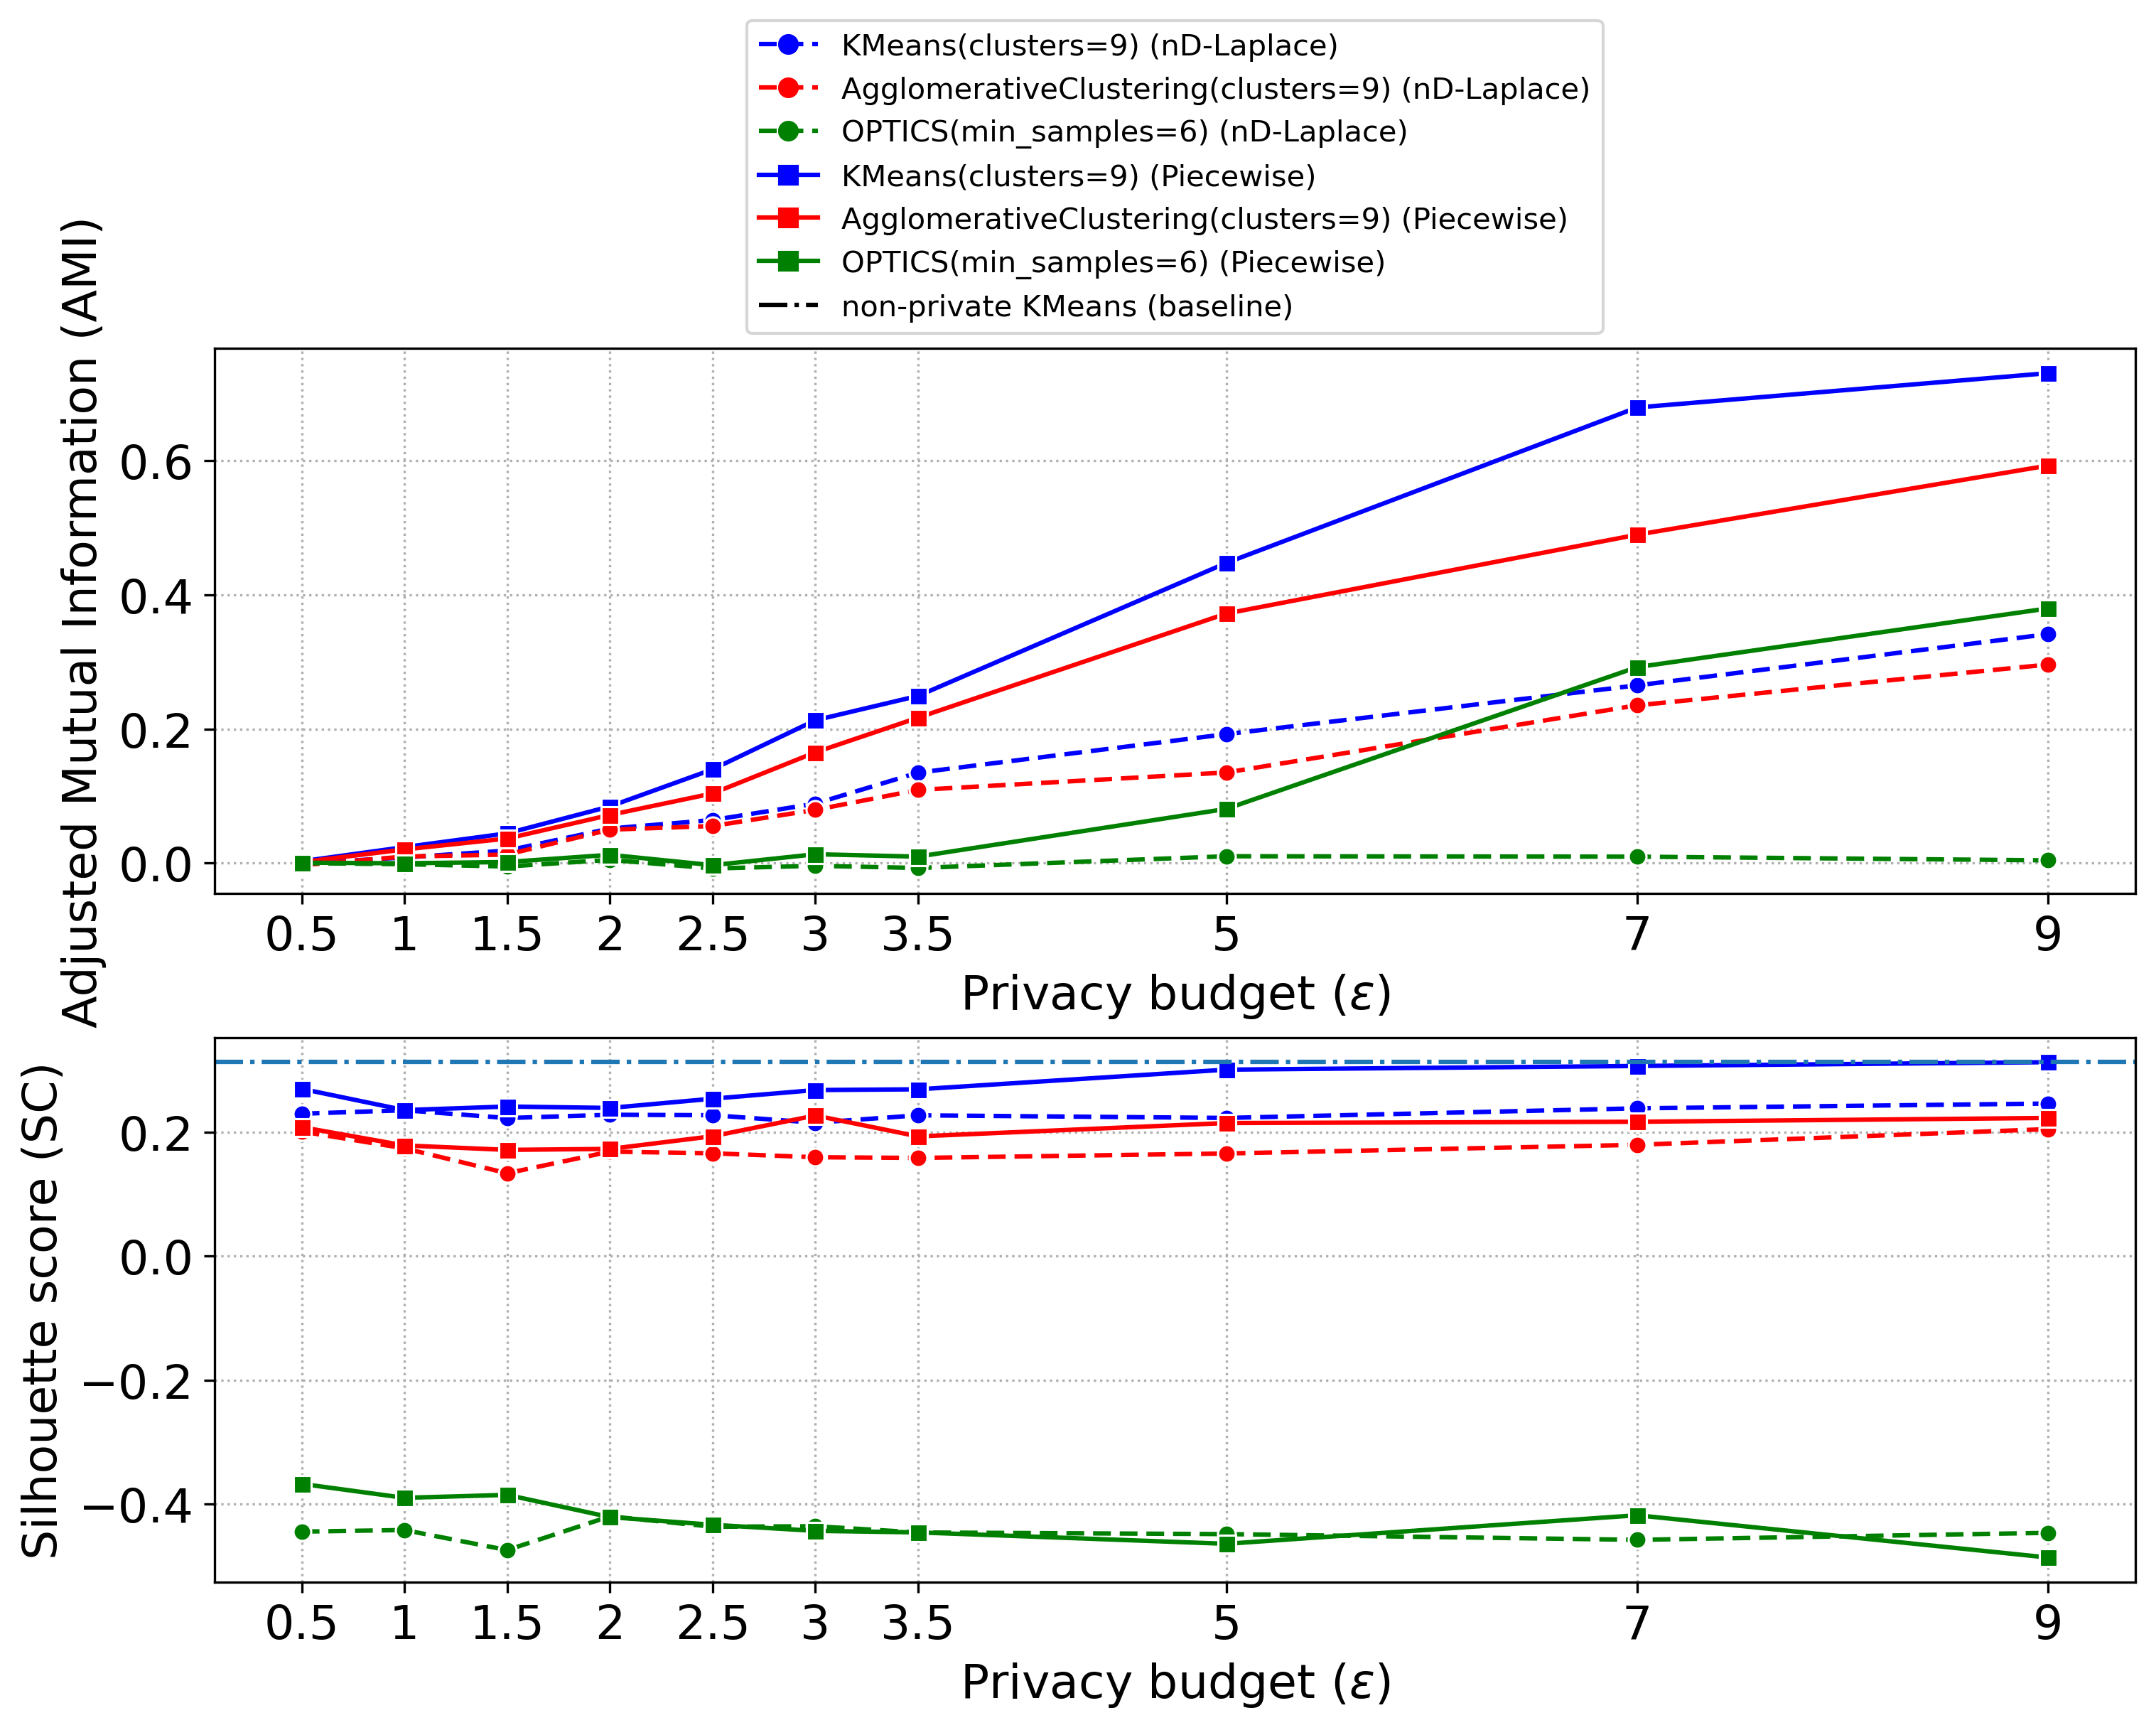
\includegraphics[width=0.9\textwidth]{Results/nd-laplace/nd-Laplace/circle-dataset/ami-and-sc_3_dimensions.png}

  \label{fig:validation-circle-dataset_comparison_3d-laplace}
\end{figure}
The nD-Laplace mechanism excels with K-Means, achieving a peak score of 0.33 \gls{ami}. While \gls{ag} closely follows, \gls{optics} lags significantly with scores less than 0.1 \gls{ami}. Similarly, the Piecewise mechanism registers its highest scores with K-Means, nearing 0.7 \gls{ami}. In this context, \gls{ag} maintains a comparable trend. Notably, \gls{optics} scores higher with Piecewise (less than 0.4 \gls{ami) than with nD-Laplace. For both mechanisms, \gls{sc} scores hover around the baseline at approximately 0.2. Across all privacy budgets, \gls{optics} consistently scores below 0 for \gls{sc}.
\todo[inline]{Discussion}
\newpage
\begin{figure}[H]
  \centering

  \caption{\textbf{AMI (top) and SC (bottom) for the kD-Laplace and Piecewise mechanisms for the 3-dimensional data line-dataset}}
  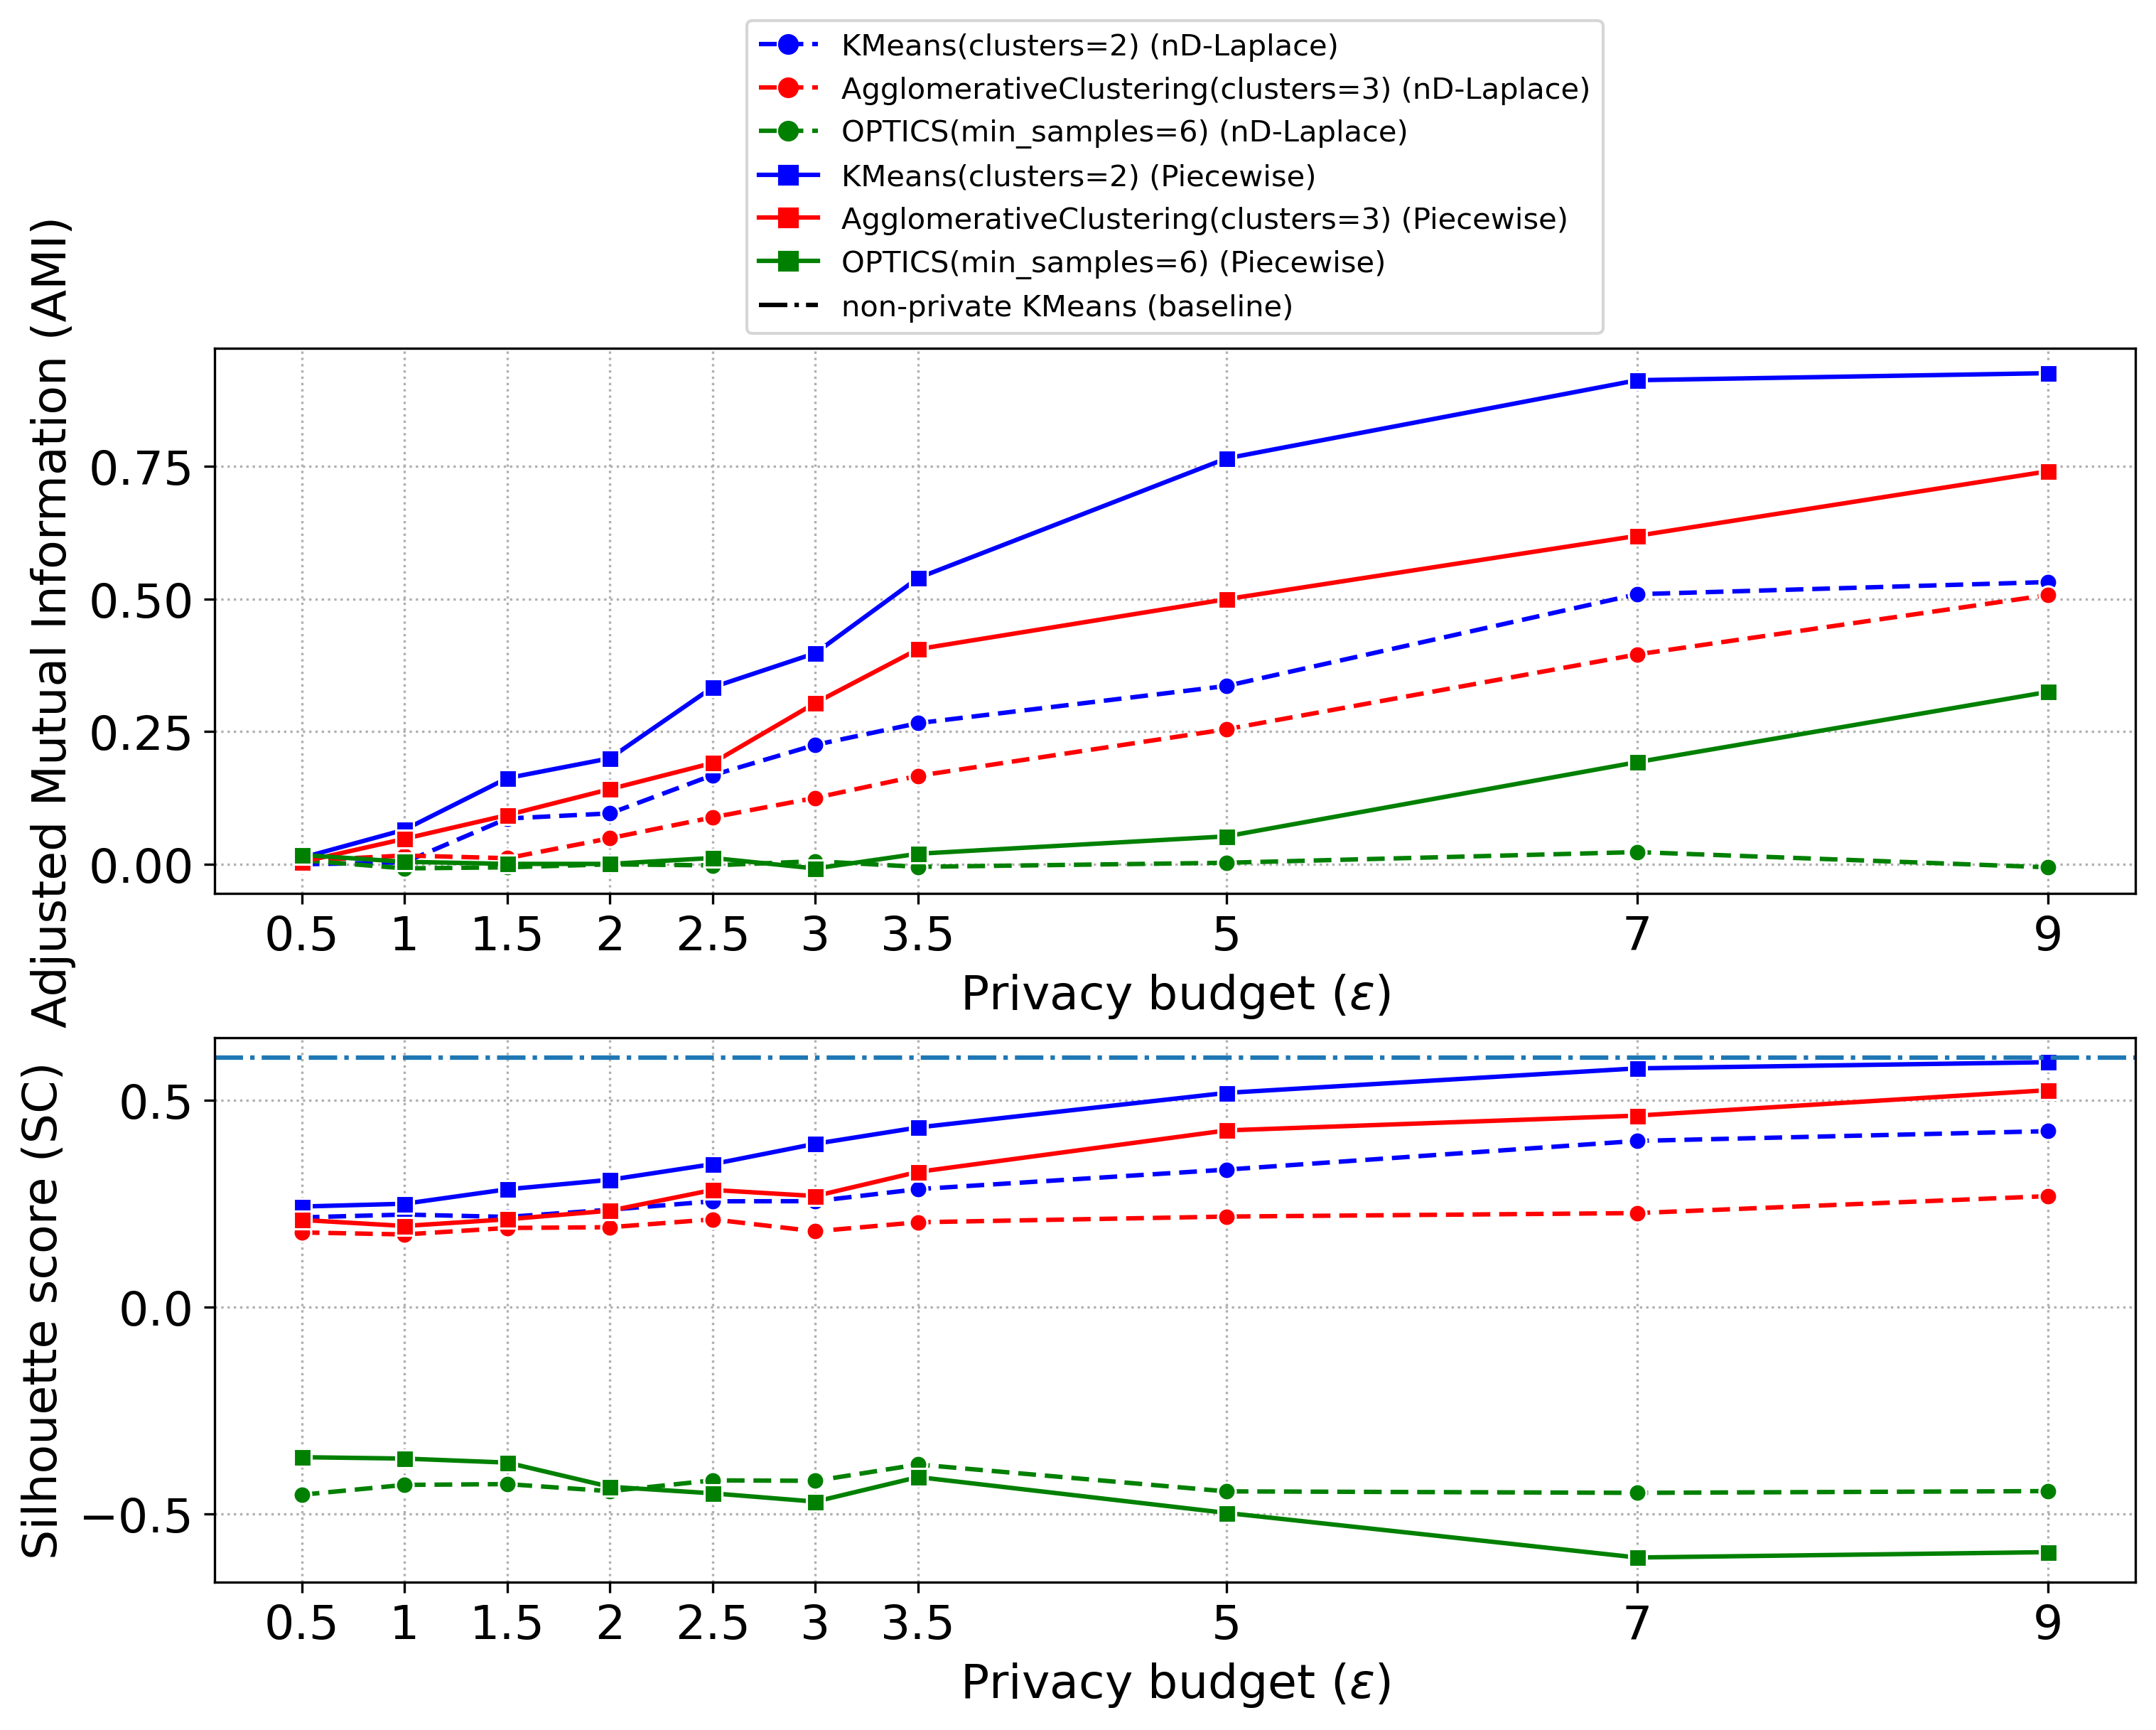
\includegraphics[width=0.9\textwidth]{Results/nd-laplace/nd-Laplace/line-dataset/ami-and-sc_3_dimensions.png}
  \label{fig:validation-line-dataset_comparison_3d-laplace}
\end{figure}
The scores in this plot closely resemble those from the previous one. With nD-Laplace, both K-Means and \gls{ag} lead the pack, though neither surpasses 0.6 \gls{ami}. Notably, \gls{optics} doesn't score at all.

The Piecewise mechanism outperforms nD-Laplace, reaching 0.86 \gls{ami} for privacy budgets at levels 7 and 9. In this scenario, \gls{ag} follows but with notably lower scores: 0.6 and 0.78 \gls{ami} for epsilon 7 and 9, respectively. While \gls{optics} remains a weaker performer across both mechanisms, it does exhibit a positive trajectory with the Piecewise mechanism.

Comparing these findings to the prior set, there are subtle variations in the \gls{sc} metric. Specifically, K-Means and \gls{ag} display a broader range of results, spanning from 0.2 to 0.6.

\newpage
\begin{figure}[H]
  \centering

  \caption{\textbf{AMI (top) and SC (bottom) for the kD-Laplace and Piecewise mechanisms for the 3-dimensional data skewed-dataset}}
  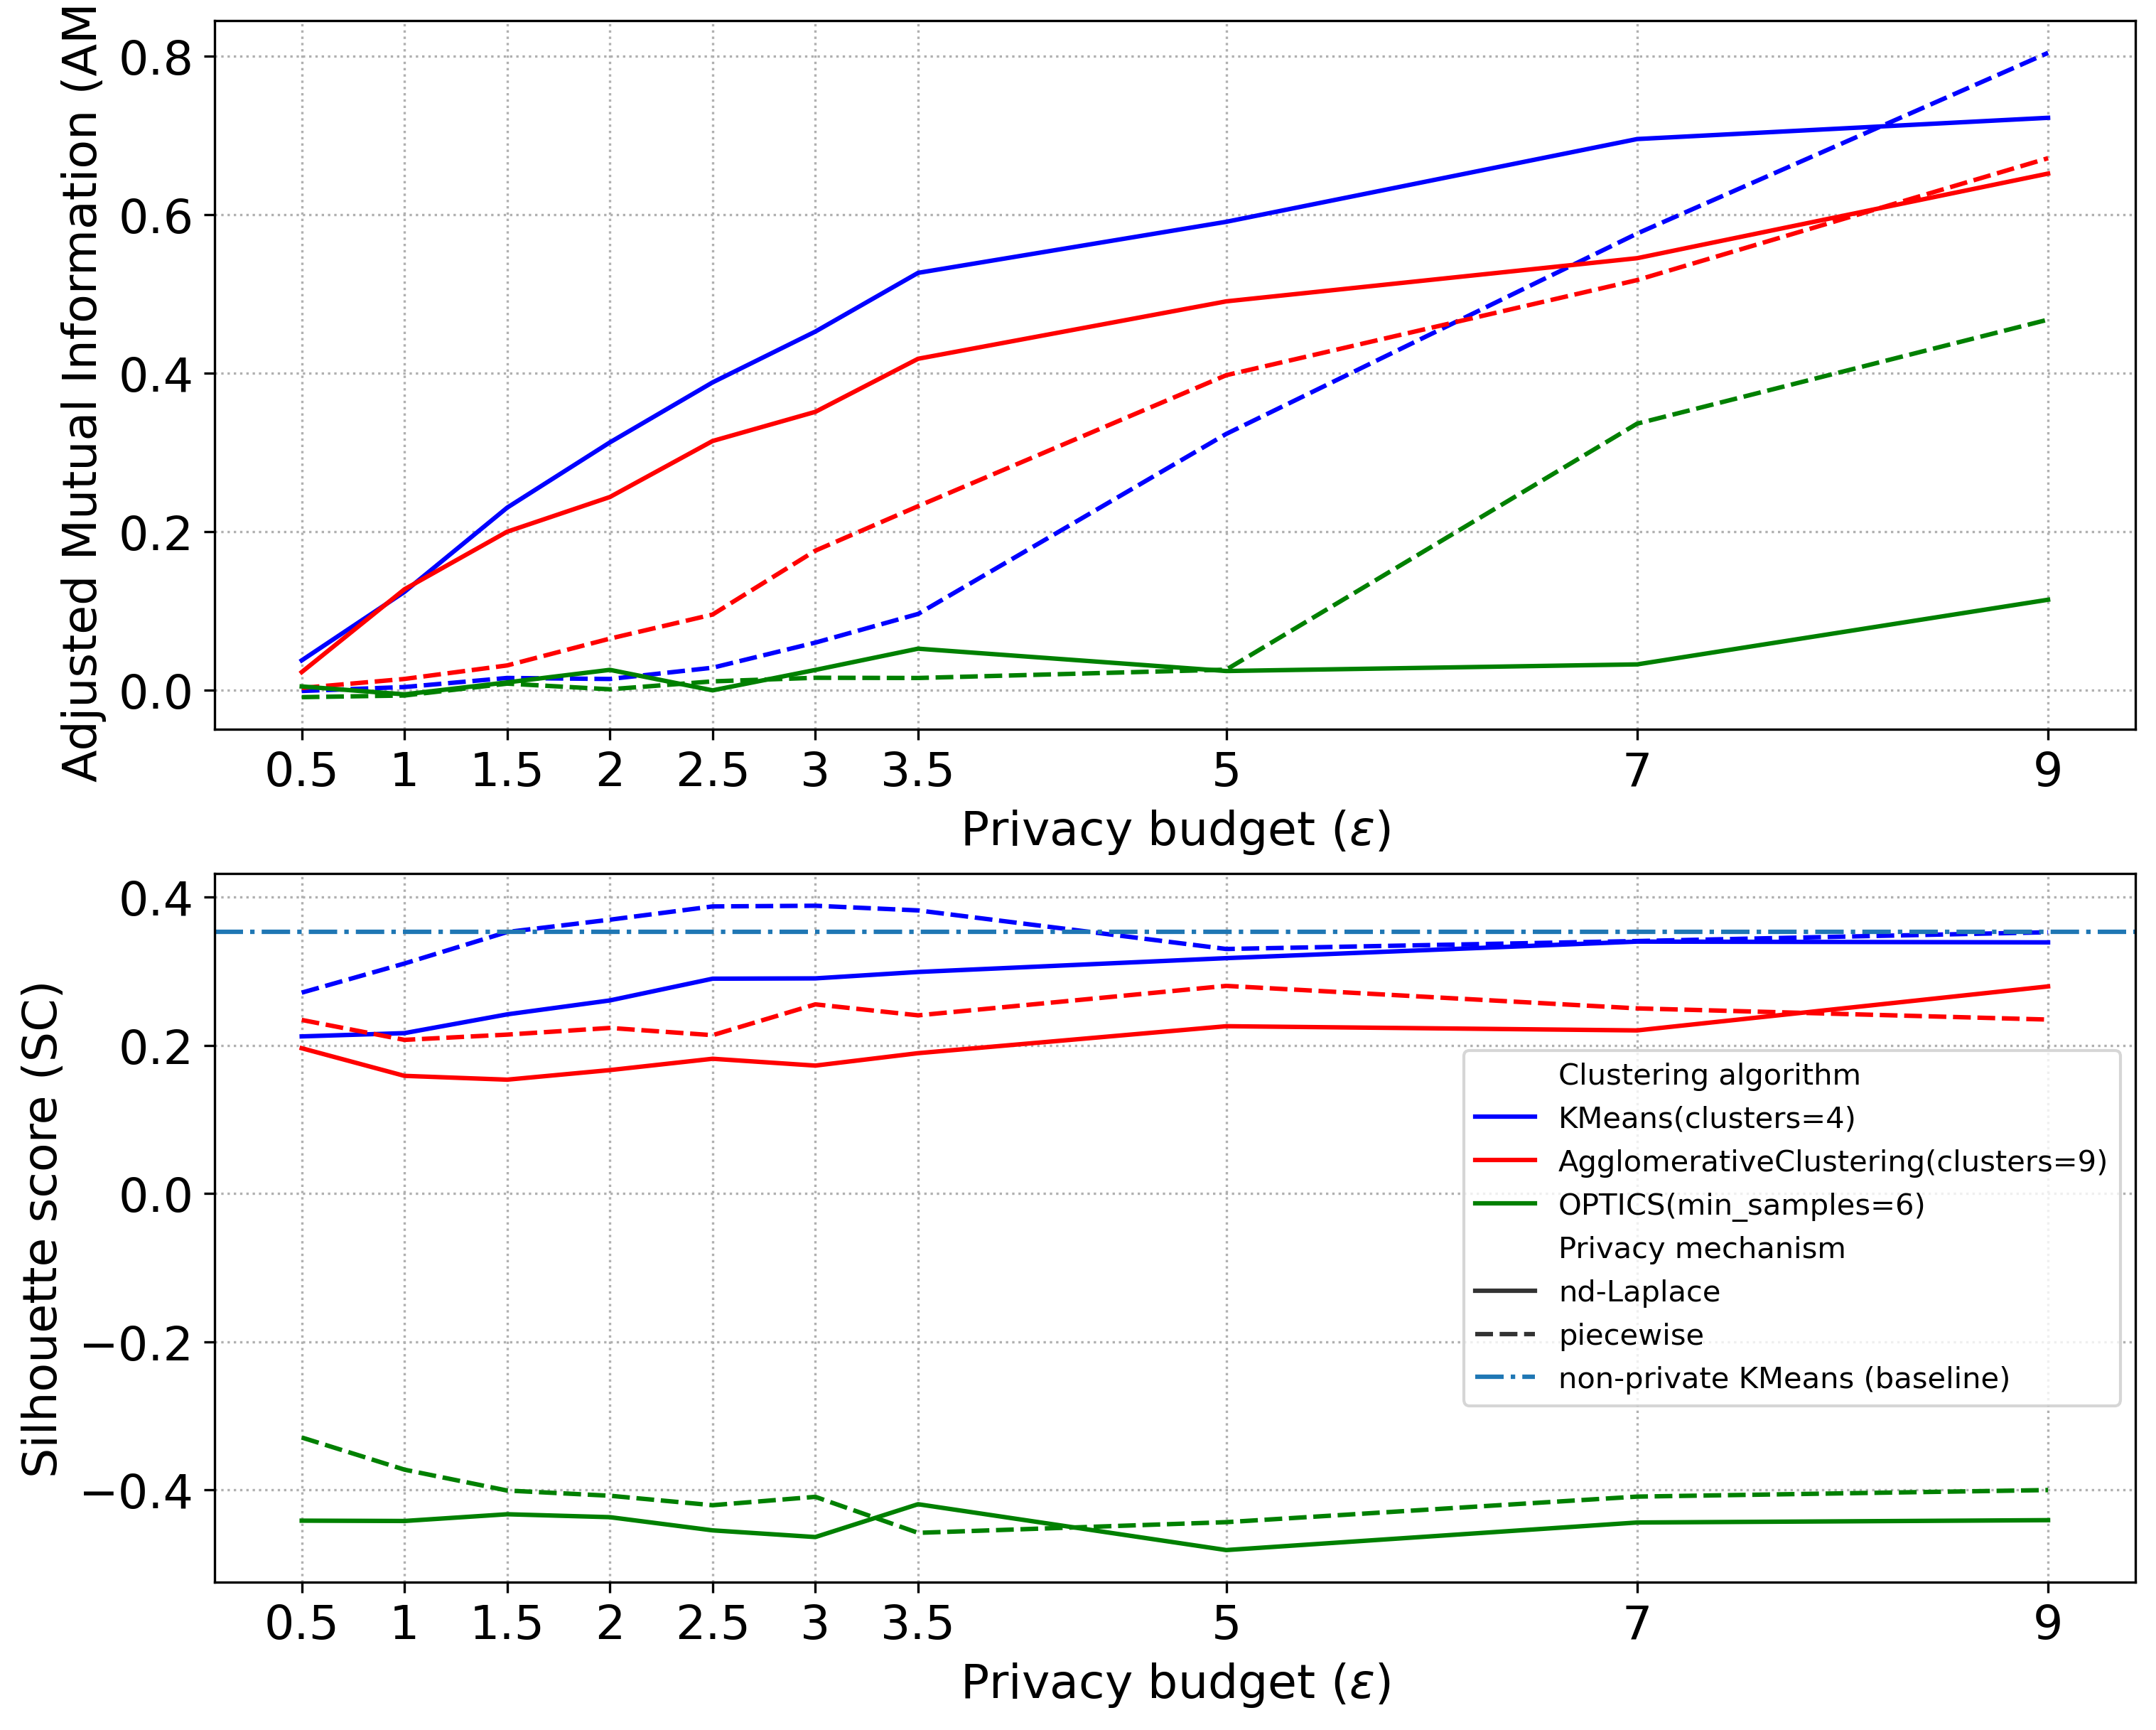
\includegraphics[width=0.9\textwidth]{Results/nd-laplace/nd-Laplace/skewed-dataset/ami-and-sc_3_dimensions.png}

  \label{fig:validation-skewed-dataset_comparison_3d-laplace}
\end{figure}
The nD-Laplace mechanism performs best with the K-Means algorithm, scoring approximately +/- 0.76 \gls{ami} for privacy budgets 7 and 9. \gls{ag} also scores well, reaching a maximum of 0.63 \gls{ami}. In contrast, \gls{optics} scores significantly lower.

For the Piecewise mechanism, we observe a similar pattern for K-Means and \gls{ag}. Although the progression of scores is alike, the actual scores only start to match from privacy budget 7 onwards. However, \gls{optics} scores much better from privacy budget 5.

For \gls{sc}, we see the same behavior, which we actually observe in every dataset. Both K-Means and \gls{ag} score close to the baseline value. In this case, \gls{ag} is slightly below K-Means.

From the results, it's evident that we see a similar trend in outcomes as with the heart-dataset. With nD-Laplace performing well at both lower and higher privacy budgets. When looking at the data distribution, it is spread out similarly to the heart-dataset. Whereas with the other datasets (especially circle/line), we noticed that the datasets have a strong shape.
\todo[inline]{Add some distribution image}.

\newpage
\subsection{n-dimensional data}
\begin{figure}[H]
  \centering

  \caption{\textbf{AMI (top) and SC (bottom) for the kD-Laplace and Piecewise mechanisms for the n-dimensional data seeds-dataset}}
  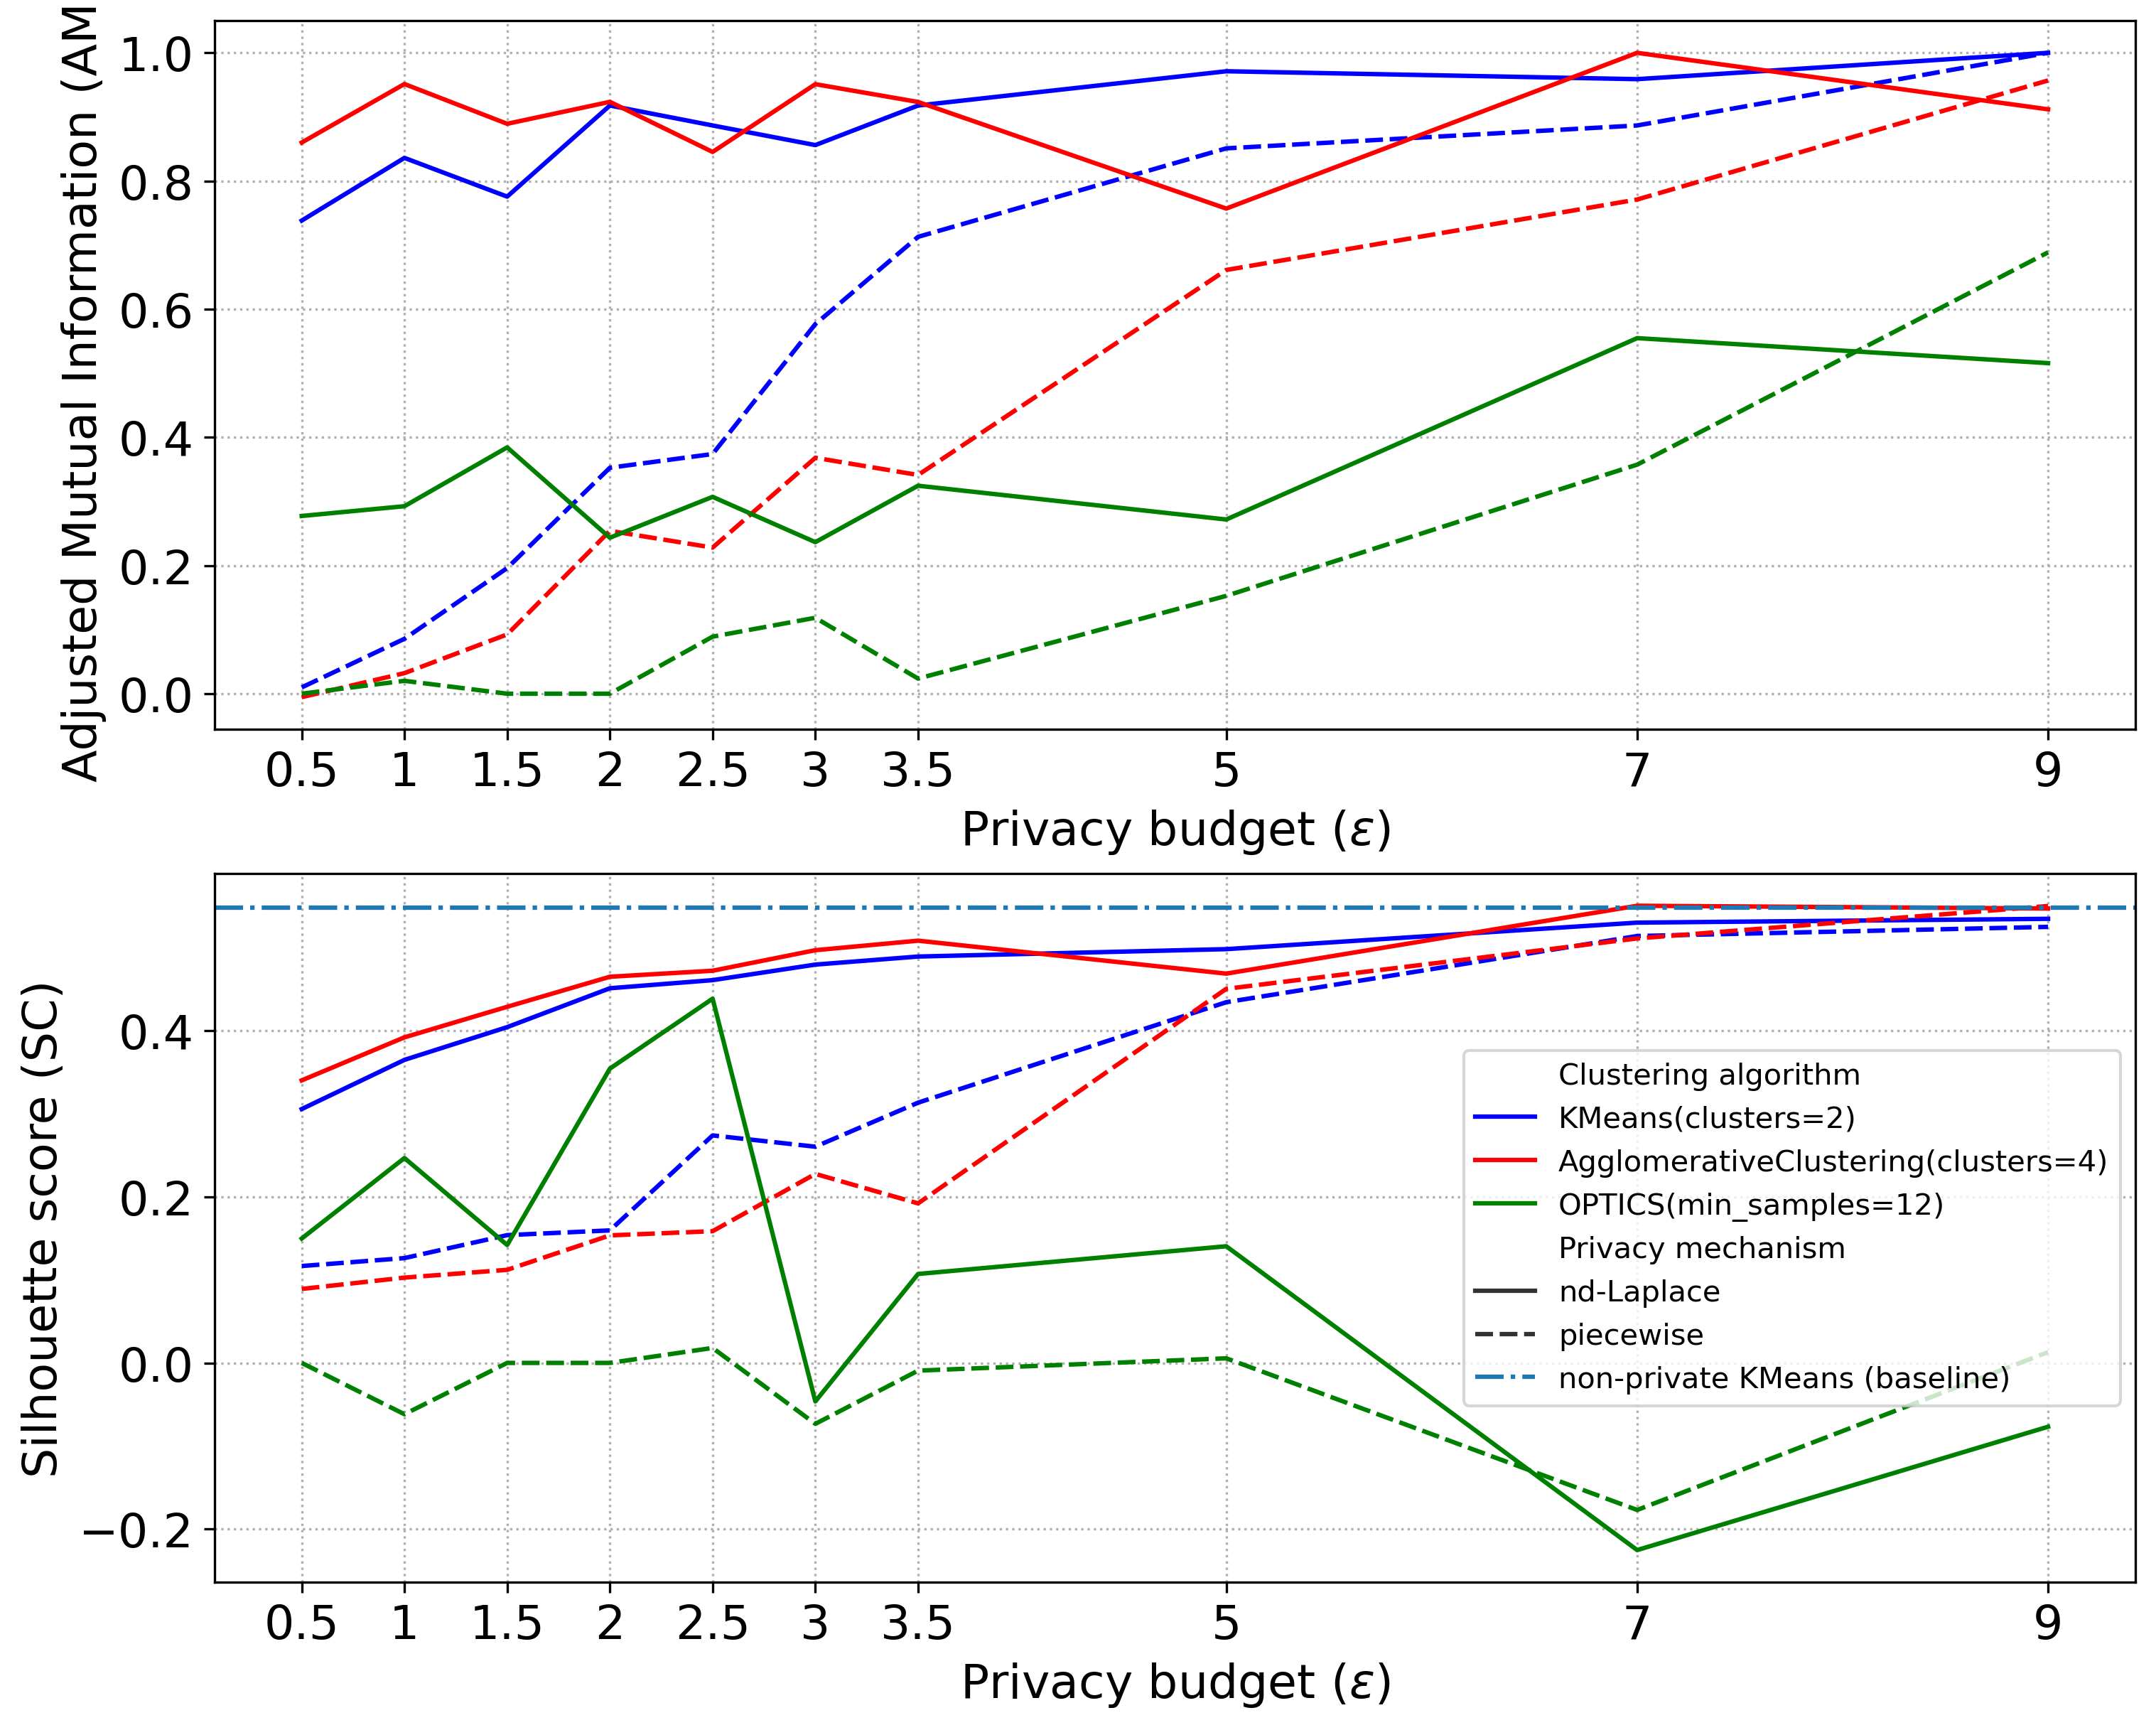
\includegraphics[width=0.9\textwidth]{Results/nd-laplace/nd-Laplace/seeds-dataset/ami-and-sc_7_dimensions.png}

  \label{fig:validation-seeds-dataset_comparison_nd-laplace}
\end{figure}
For n-dimensional data, we observe that nD-Laplace consistently scores high from privacy budget 0.5 up to 9. This applies to both K-Means and \gls{ag}. \gls{optics} also shows some improvements, scoring between 0.25 and 0.55 from epsilon 0.5 to 9.

The Piecewise mechanism only starts to show comparable results from a privacy budget of 5. From that point on, the results for K-Means and \gls{ag} are almost identical. For \gls{optics}, Piecewise scores slightly higher at a privacy budget of 9, but for the other privacy budgets, nD-Laplace performs better.

For \gls{sc}, we see a bit more variation between the mechanisms than with the other dimensions. Also, The trend of \gls{sc} seems more similar to that of \gls{ami} than what we've observed in other dimensions. 
Looking at the scores, the nD-Laplace mechanism scores below the baseline from privacy budgets 0.5 to 7 but matches the scores for K-Means and \gls{ag} afterward. For nD-Laplace, \gls{optics} starts at 0.2 \gls{sc}, but then drops below 0. The Piecewise mechanism remains below 0 for \gls{optics} across all privacy budgets.

Something notable occurs for the privacy budget of 2.5, as \gls{optics} peaks at 2.5. We would only expect this at a privacy budget of 9 when less noise has been added.
\todo[inline]{We have to research this.}
\newpage
\begin{figure}[H]
  \centering

  \caption{\textbf{AMI (top) and SC (bottom) for the kD-Laplace and Piecewise mechanisms for the n-dimensional data heart-dataset}}
  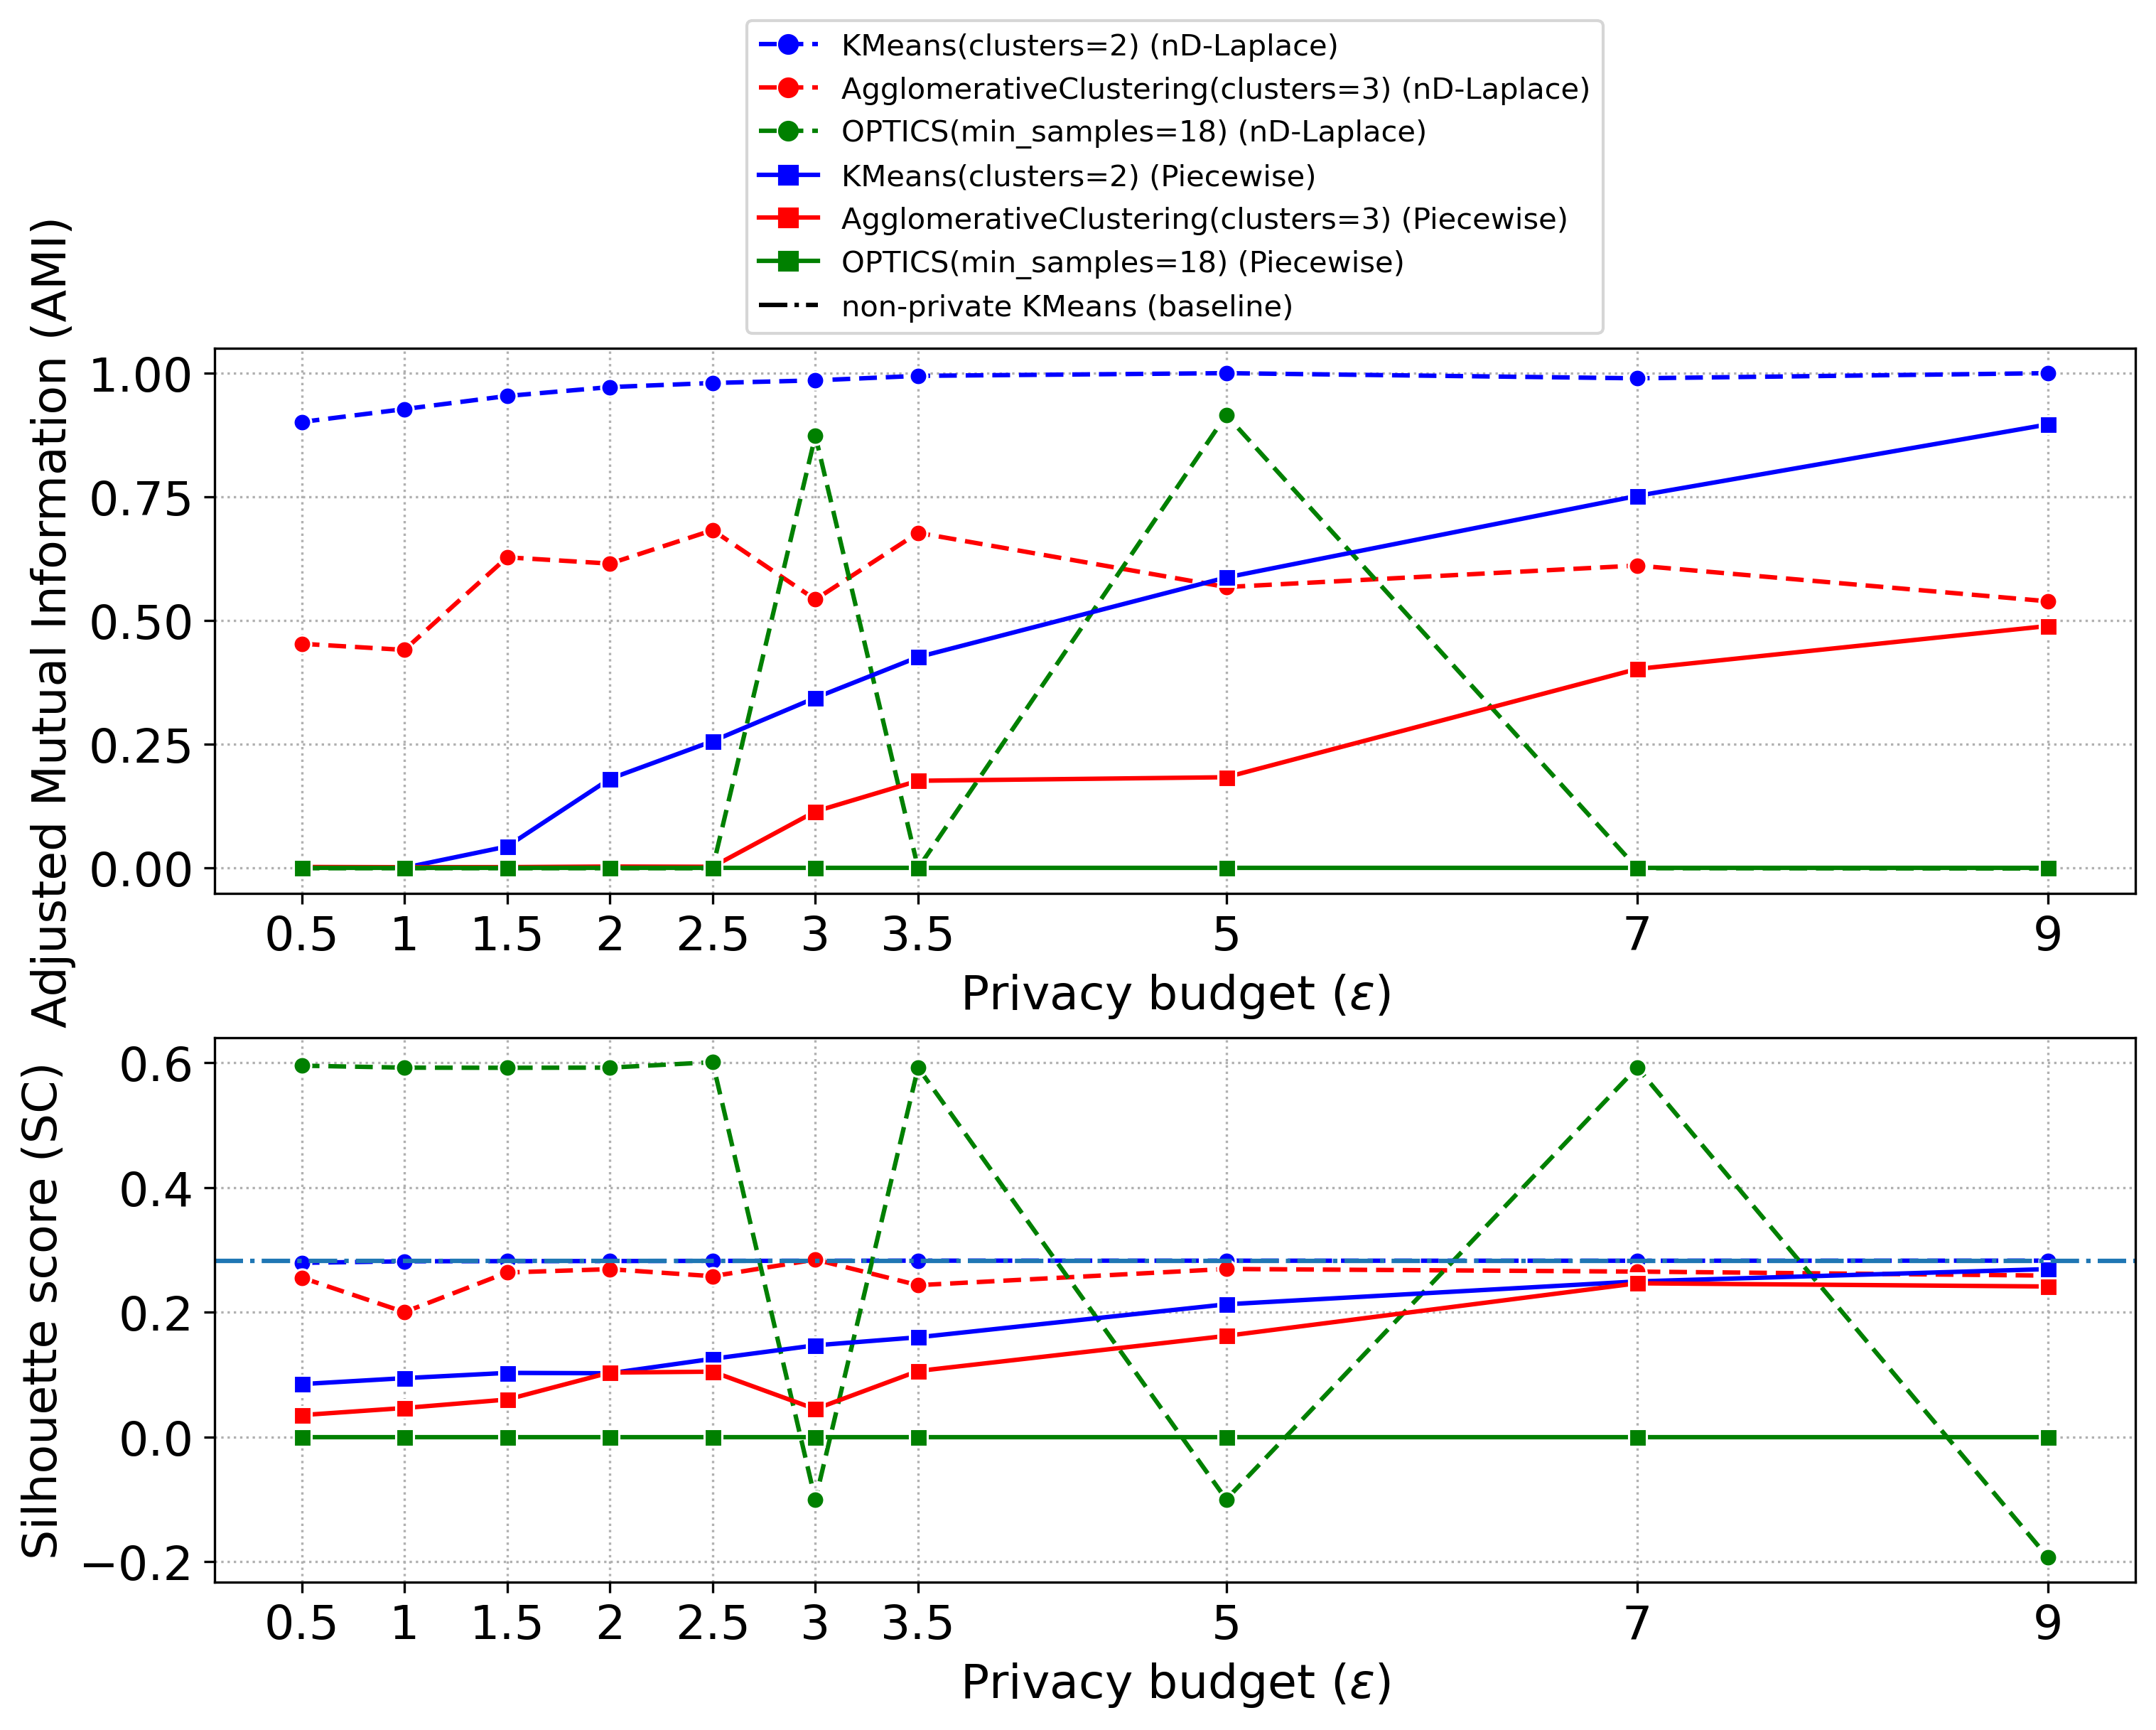
\includegraphics[width=0.9\textwidth]{Results/nd-laplace/nd-Laplace/heart-dataset/ami-and-sc_9_dimensions.png}

  \label{fig:validation-heart-dataset_comparison_nd-laplace}
\end{figure}
For nD-Laplace, the heart-dataset consistently scores very well for K-Means. Even for n-dimensional data, the result consistently remains above 0.95 \gls{ami} for all privacy budgets.
For \gls{ag}, a good score is achieved, but it plateaus around 0.6 \gls{ami}.
With \gls{optics}, the data is quite inconsistent, ranging from 0 to 0.90 \gls{ami}.
The Piecewise mechanism shows a similar trend for both K-Means and \gls{ag}, with K-Means performing the best. Both score below nD-Laplace across all privacy budgets.
For \gls{optics}, the score remains at 0 for the Piecewise mechanism.
With the \gls{sc} metric, the same pattern is evident, but the \gls{sc} is relatively low when considering the high \gls{ami} achieved. For \gls{optics}, an odd result is observed, as it scores 0.6 \gls{ami} (0.25 above the baseline) from 0.5 to 3. However, for privacy budgets of 3, 5, and 9, the score drops back to 0 \gls{sc}.

\todo[inline]{Analyse gedrag}

\newpage
\section{Mechanism utility}
The sections below present a heatmap comparison of the nd-Laplace and Piecewise mechanisms.
We employed a heatmap to simultaneously depict the privacy budget (epsilon), the number of dimensions, and a specific metric. The metric in focus is the \gls{ami}, which is determined using the K-Means algorithm.
We opted for K-Means as it consistently delivered reliable results across all our experiments, making it an ideal baseline for gauging the \gls{ami}.

On the heatmap, the x-axis represents the privacy budget, while the y-axis illustrates the number of dimensions. Each cell of the heatmap conveys the \gls{ami} value. The intensity of the cell's color corresponds to the \gls{ami} score: a darker shade signifies a higher score. Consequently, the darker (or higher) the score, the more favorable the outcome. \newline

The results for the shape datasets (Circle, Line and Skewed) were omitted, because we do not have more then 3 dimensions. Therefore, the heat maps do not yield a lot of information in addition to the cluster utility plots.

Please refer to the plots in the appendix for:
\begin{enumerate}
  \item Privacy distance: \ref{appendix:results-privacy}.
  \item True Positive Rate: \ref{appendix:results-privacy}.
\end{enumerate}
\newpage
\subsection{Seeds-dataset}
\begin{figure}[H]
  \centering
  \begin{subfigure}[b]{0.8\textwidth}
    \begin{subfigure}[c]{1\textwidth}
      \caption{\textbf{Adjusted Mutual Information comparison for the kd-Laplace mechanism}}
      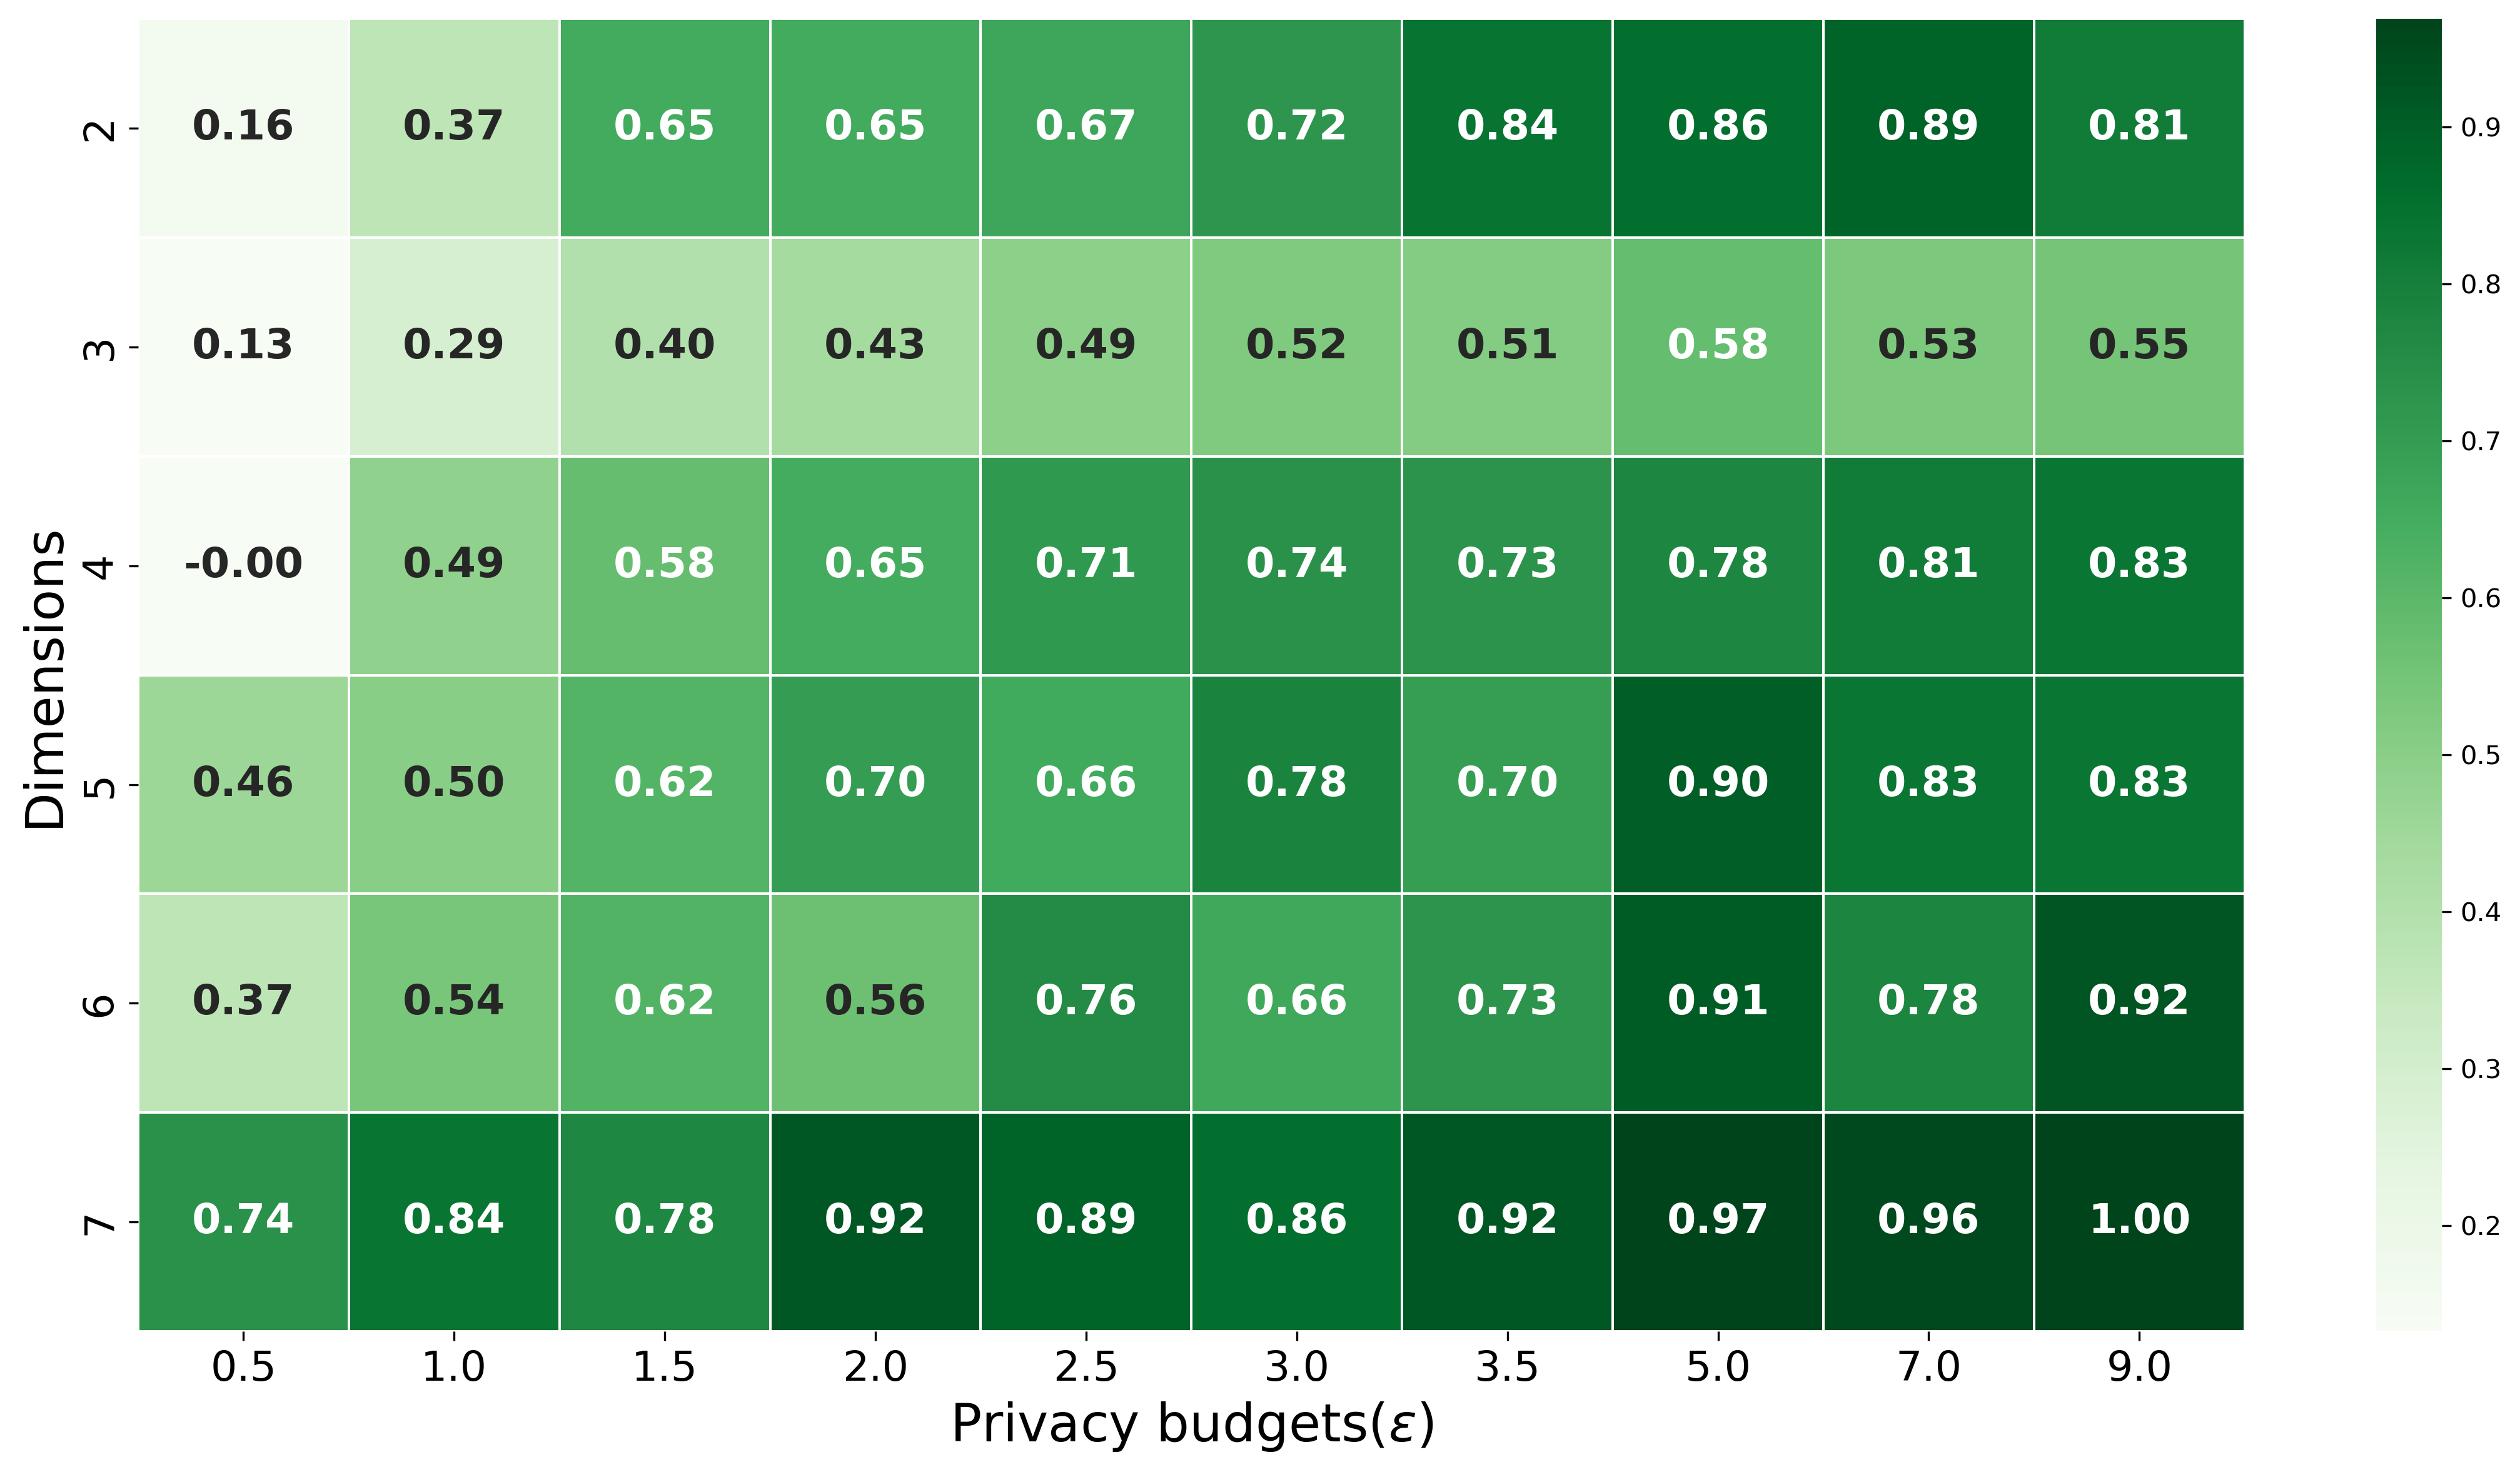
\includegraphics[width=1\textwidth]{Results/nd-laplace/nd-Laplace/seeds-dataset/ami.png}
      \label{fig:ami_seeds-dataset_comparison_kdlaplace_2d}
    \end{subfigure}
    \vfill % vertical space
    \begin{subfigure}[c]{1\textwidth}
      \caption{\textbf{Adjusted Mutual Information comparison for the Piecewise mechanism}}
      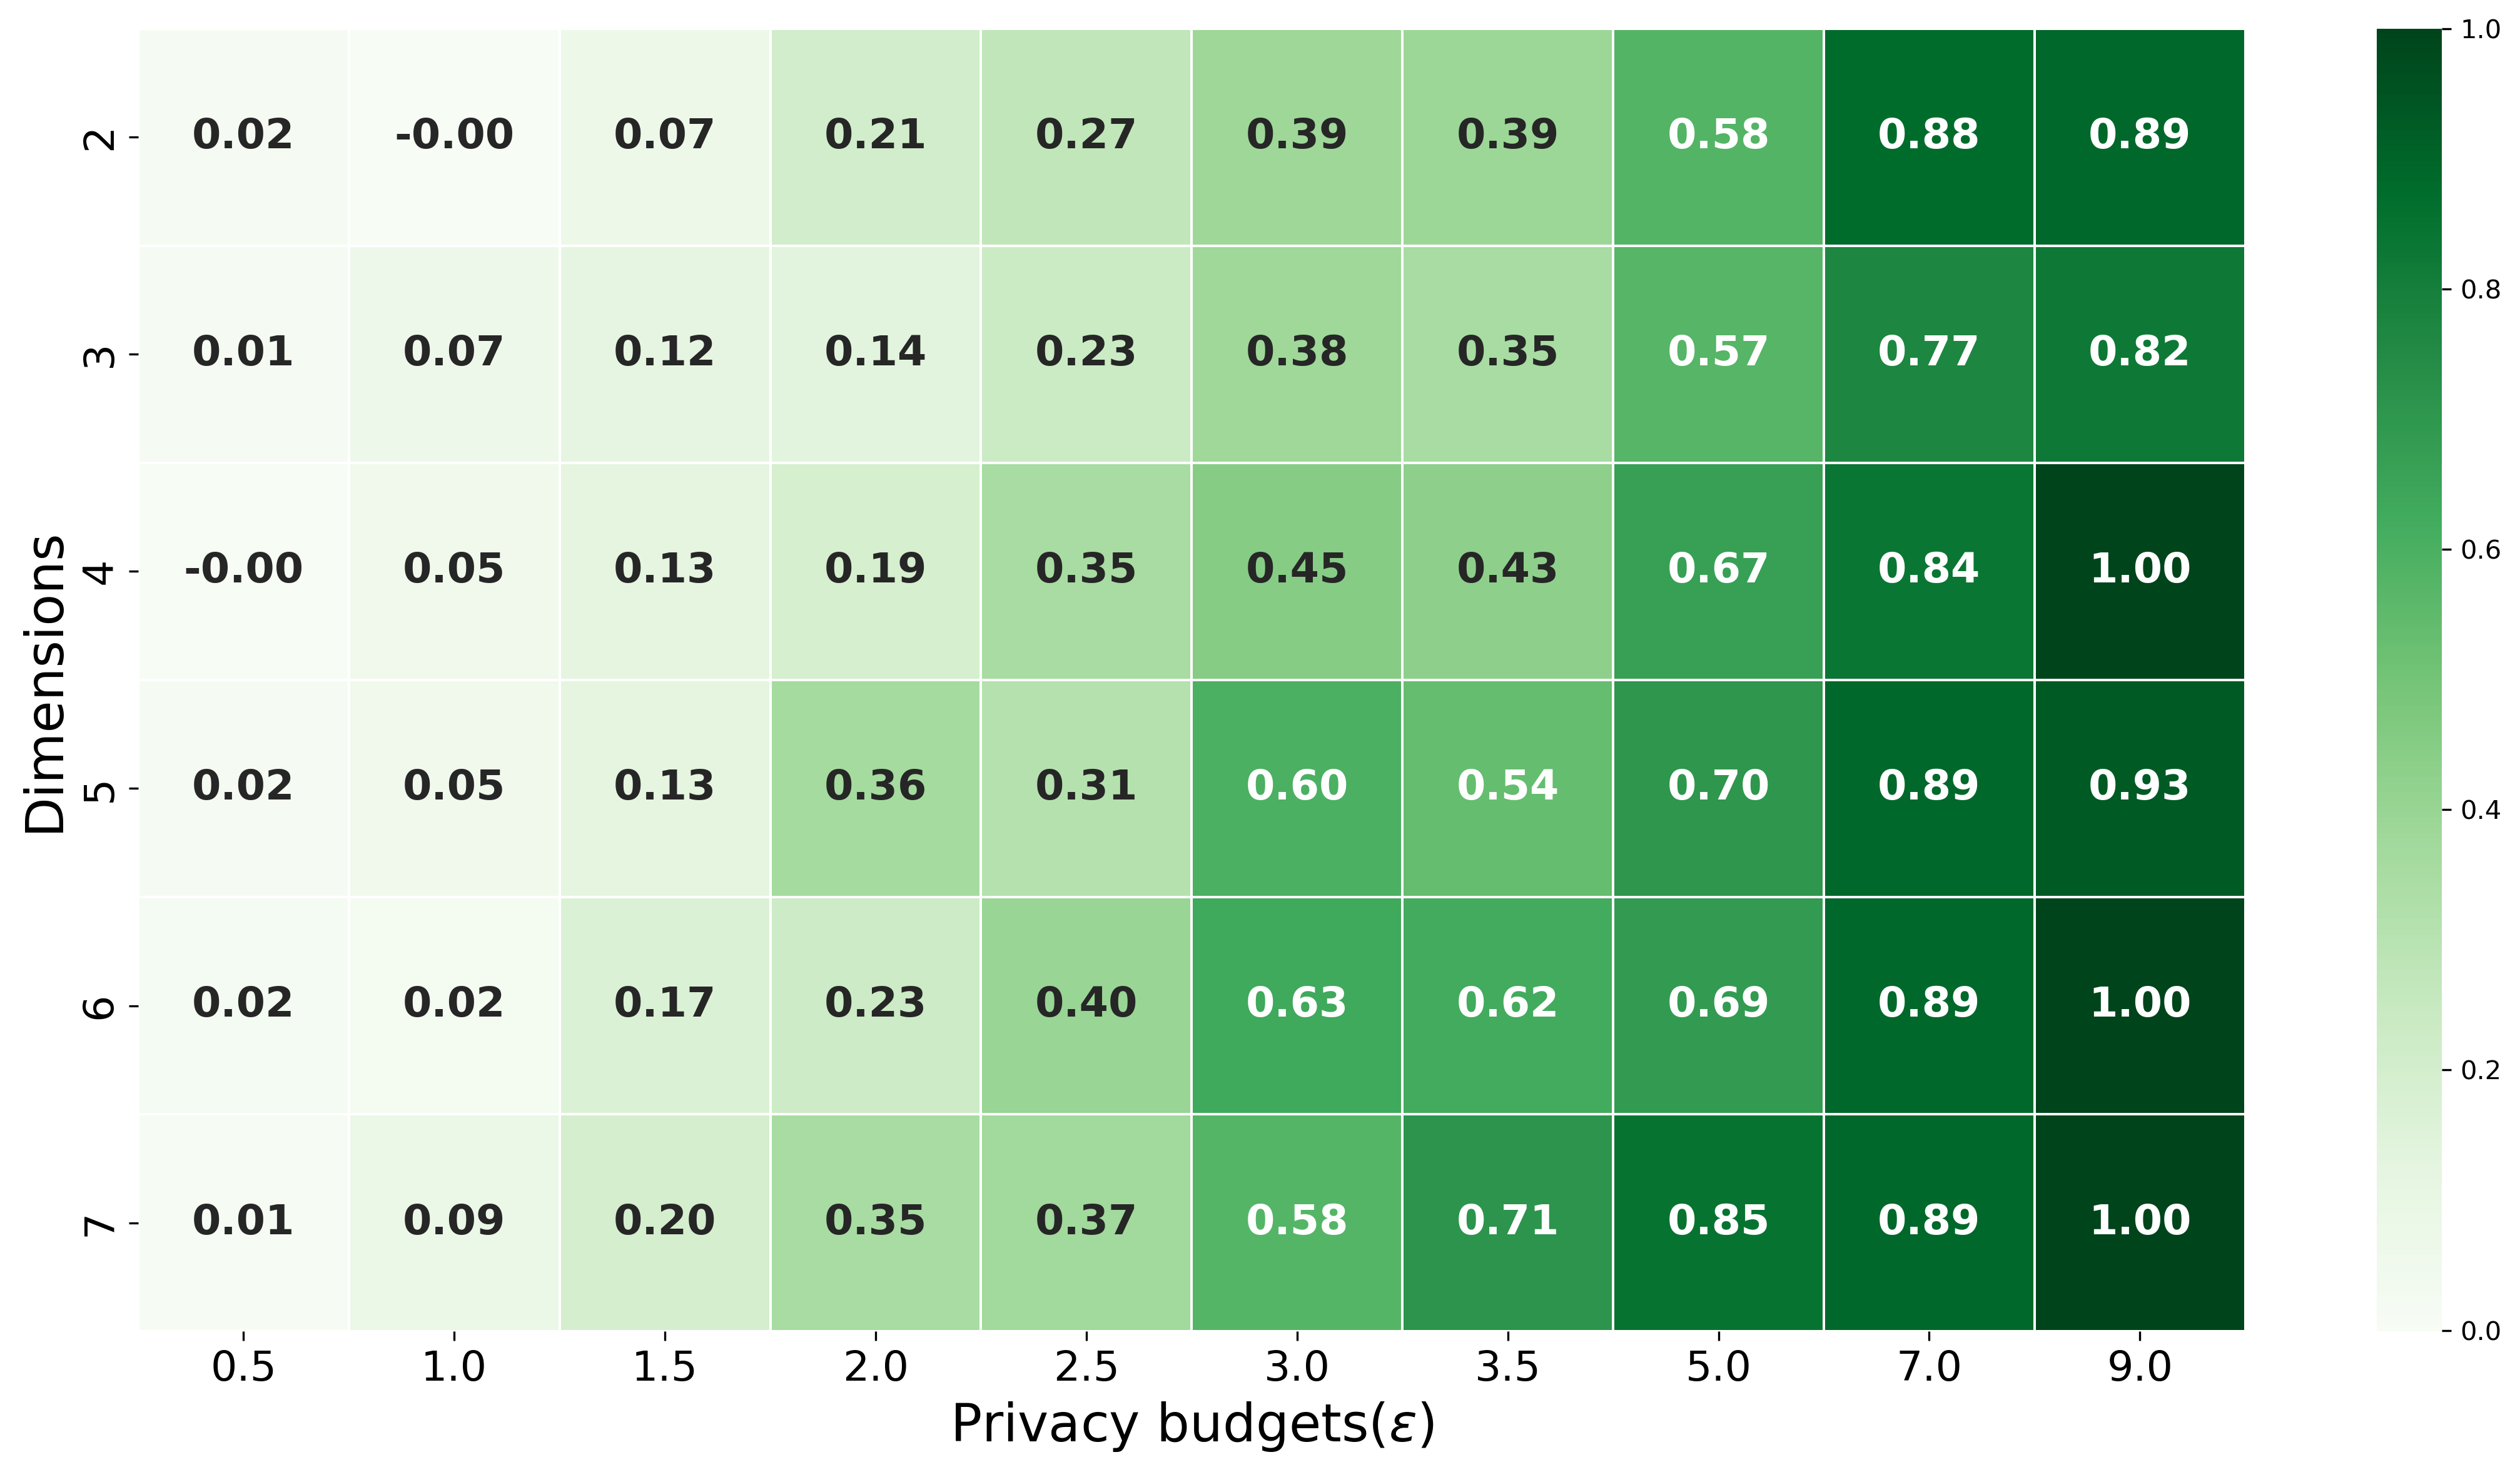
\includegraphics[width=1\textwidth]{Results/nd-laplace/piecewise/seeds-dataset/ami.png}
      \label{fig:ami_seeds-dataset_comparison_piecewise_2d}
    \end{subfigure}
  \end{subfigure}
  
\end{figure}
For the heatmaps, we observe a similar pattern, which was also evident in the cluster analysis. Specifically, nD-Laplace consistently scores well from lower epsilons, while Piecewise only starts to perform well from a privacy budget of 3.
For nD-Laplace, the number of dimensions influences the score. The implementation of 3D-Laplace, in particular, scores relatively low. From 4 dimensions onward, we notice an increase in the \gls{ami}, especially in combination with an increasing \gls{epsilon}.
For Piecewise, it's notable that the number of dimensions has minimal impact on the outcome, with the privacy budget being the primary influencing factor. However, dimension does play a role for privacy budgets between 3 and 5, as scores are higher from 5 dimensions compared to lower dimensions.

For nD-Laplace, the dimensions can significantly influence the improved result because as the number of dimensions increases, the noise decreases. We've elaborated on this phenomenon in Section \ref{fig:curse-of-dimensionality}. As a result, more information is retained, leading to an increase in score with the number of dimensions. The Piecewise mechanism might also be affected by this, but to a lesser extent.
\todo[inline]{Further research needed}

\newpage
\subsection{Heart-dataset}
\begin{figure}[H]
  \centering
  \begin{subfigure}[b]{0.80\textwidth}
    \begin{subfigure}[c]{1\textwidth}
      \caption{\textbf{Adjusted Mutual Information comparison for the kd-Laplace mechanism}}
      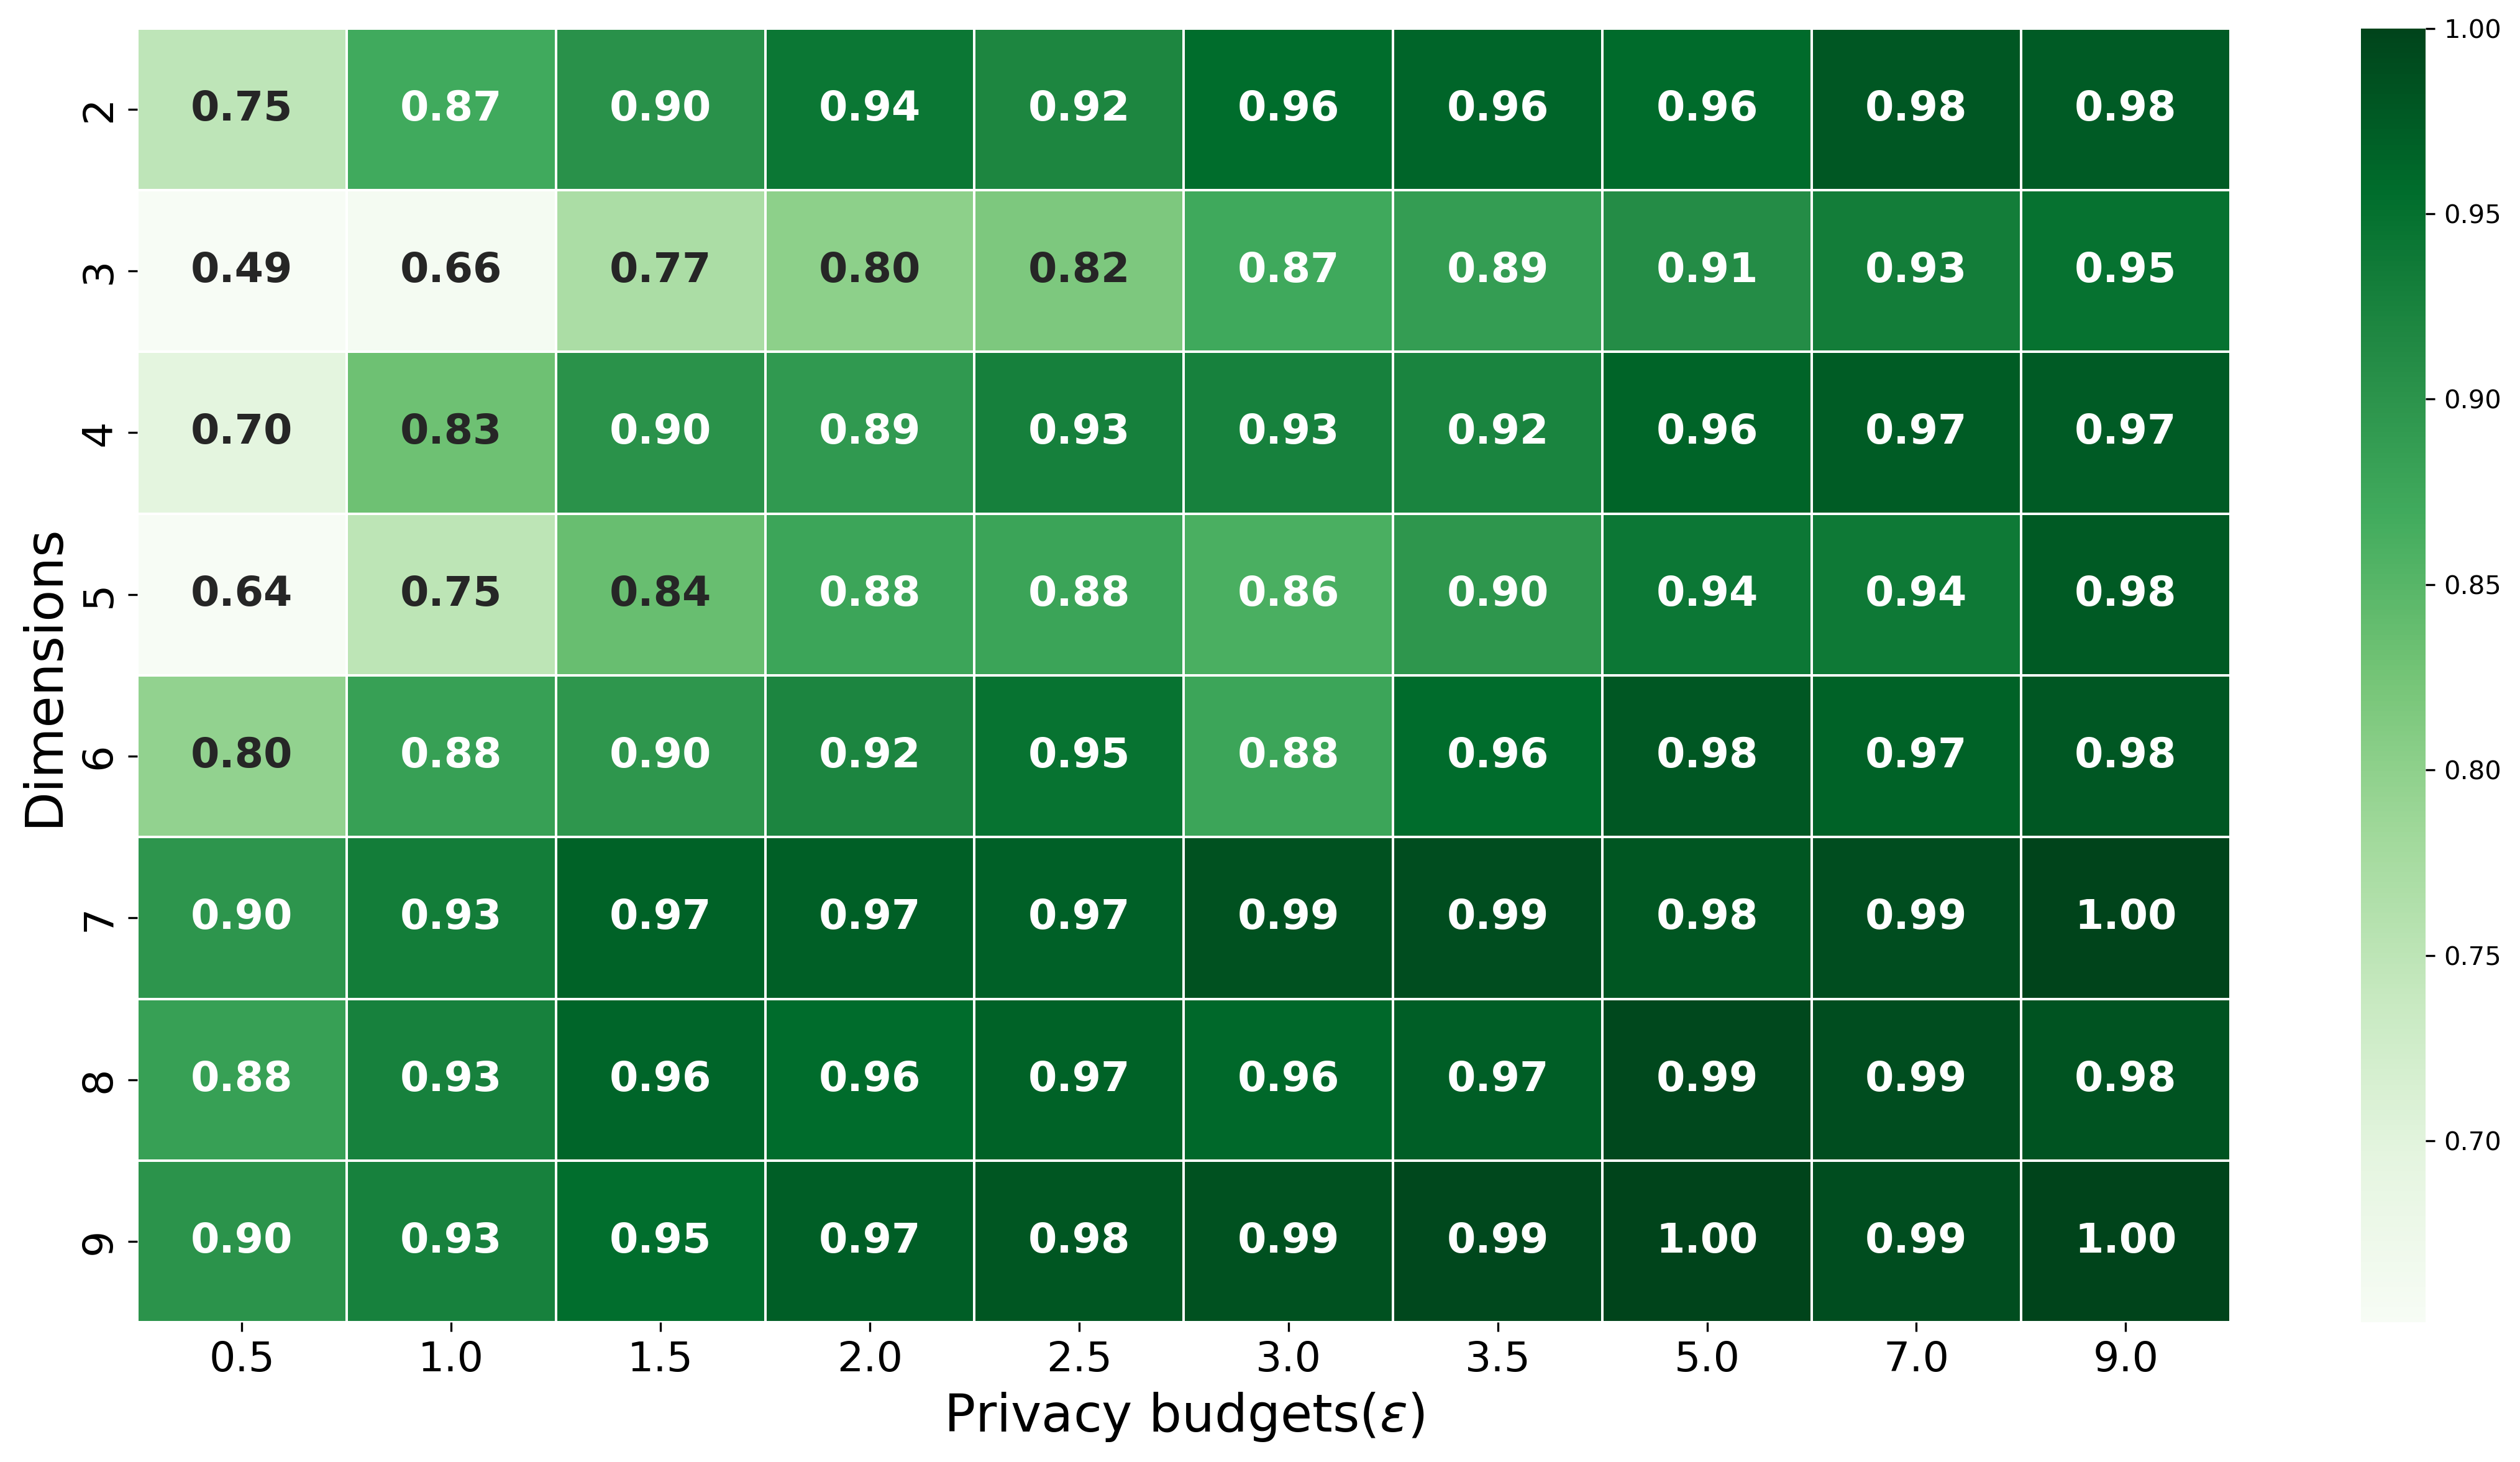
\includegraphics[width=1\textwidth]{Results/nd-laplace/nd-Laplace/heart-dataset/ami.png}
      \label{fig:ami_heart-dataset_comparison_kdlaplace_2d}
    \end{subfigure}
    \vfill % vertical space
    \begin{subfigure}[c]{1\textwidth}
      \caption{\textbf{Adjusted Mutual Information comparison for the Piecewise mechanism}}
      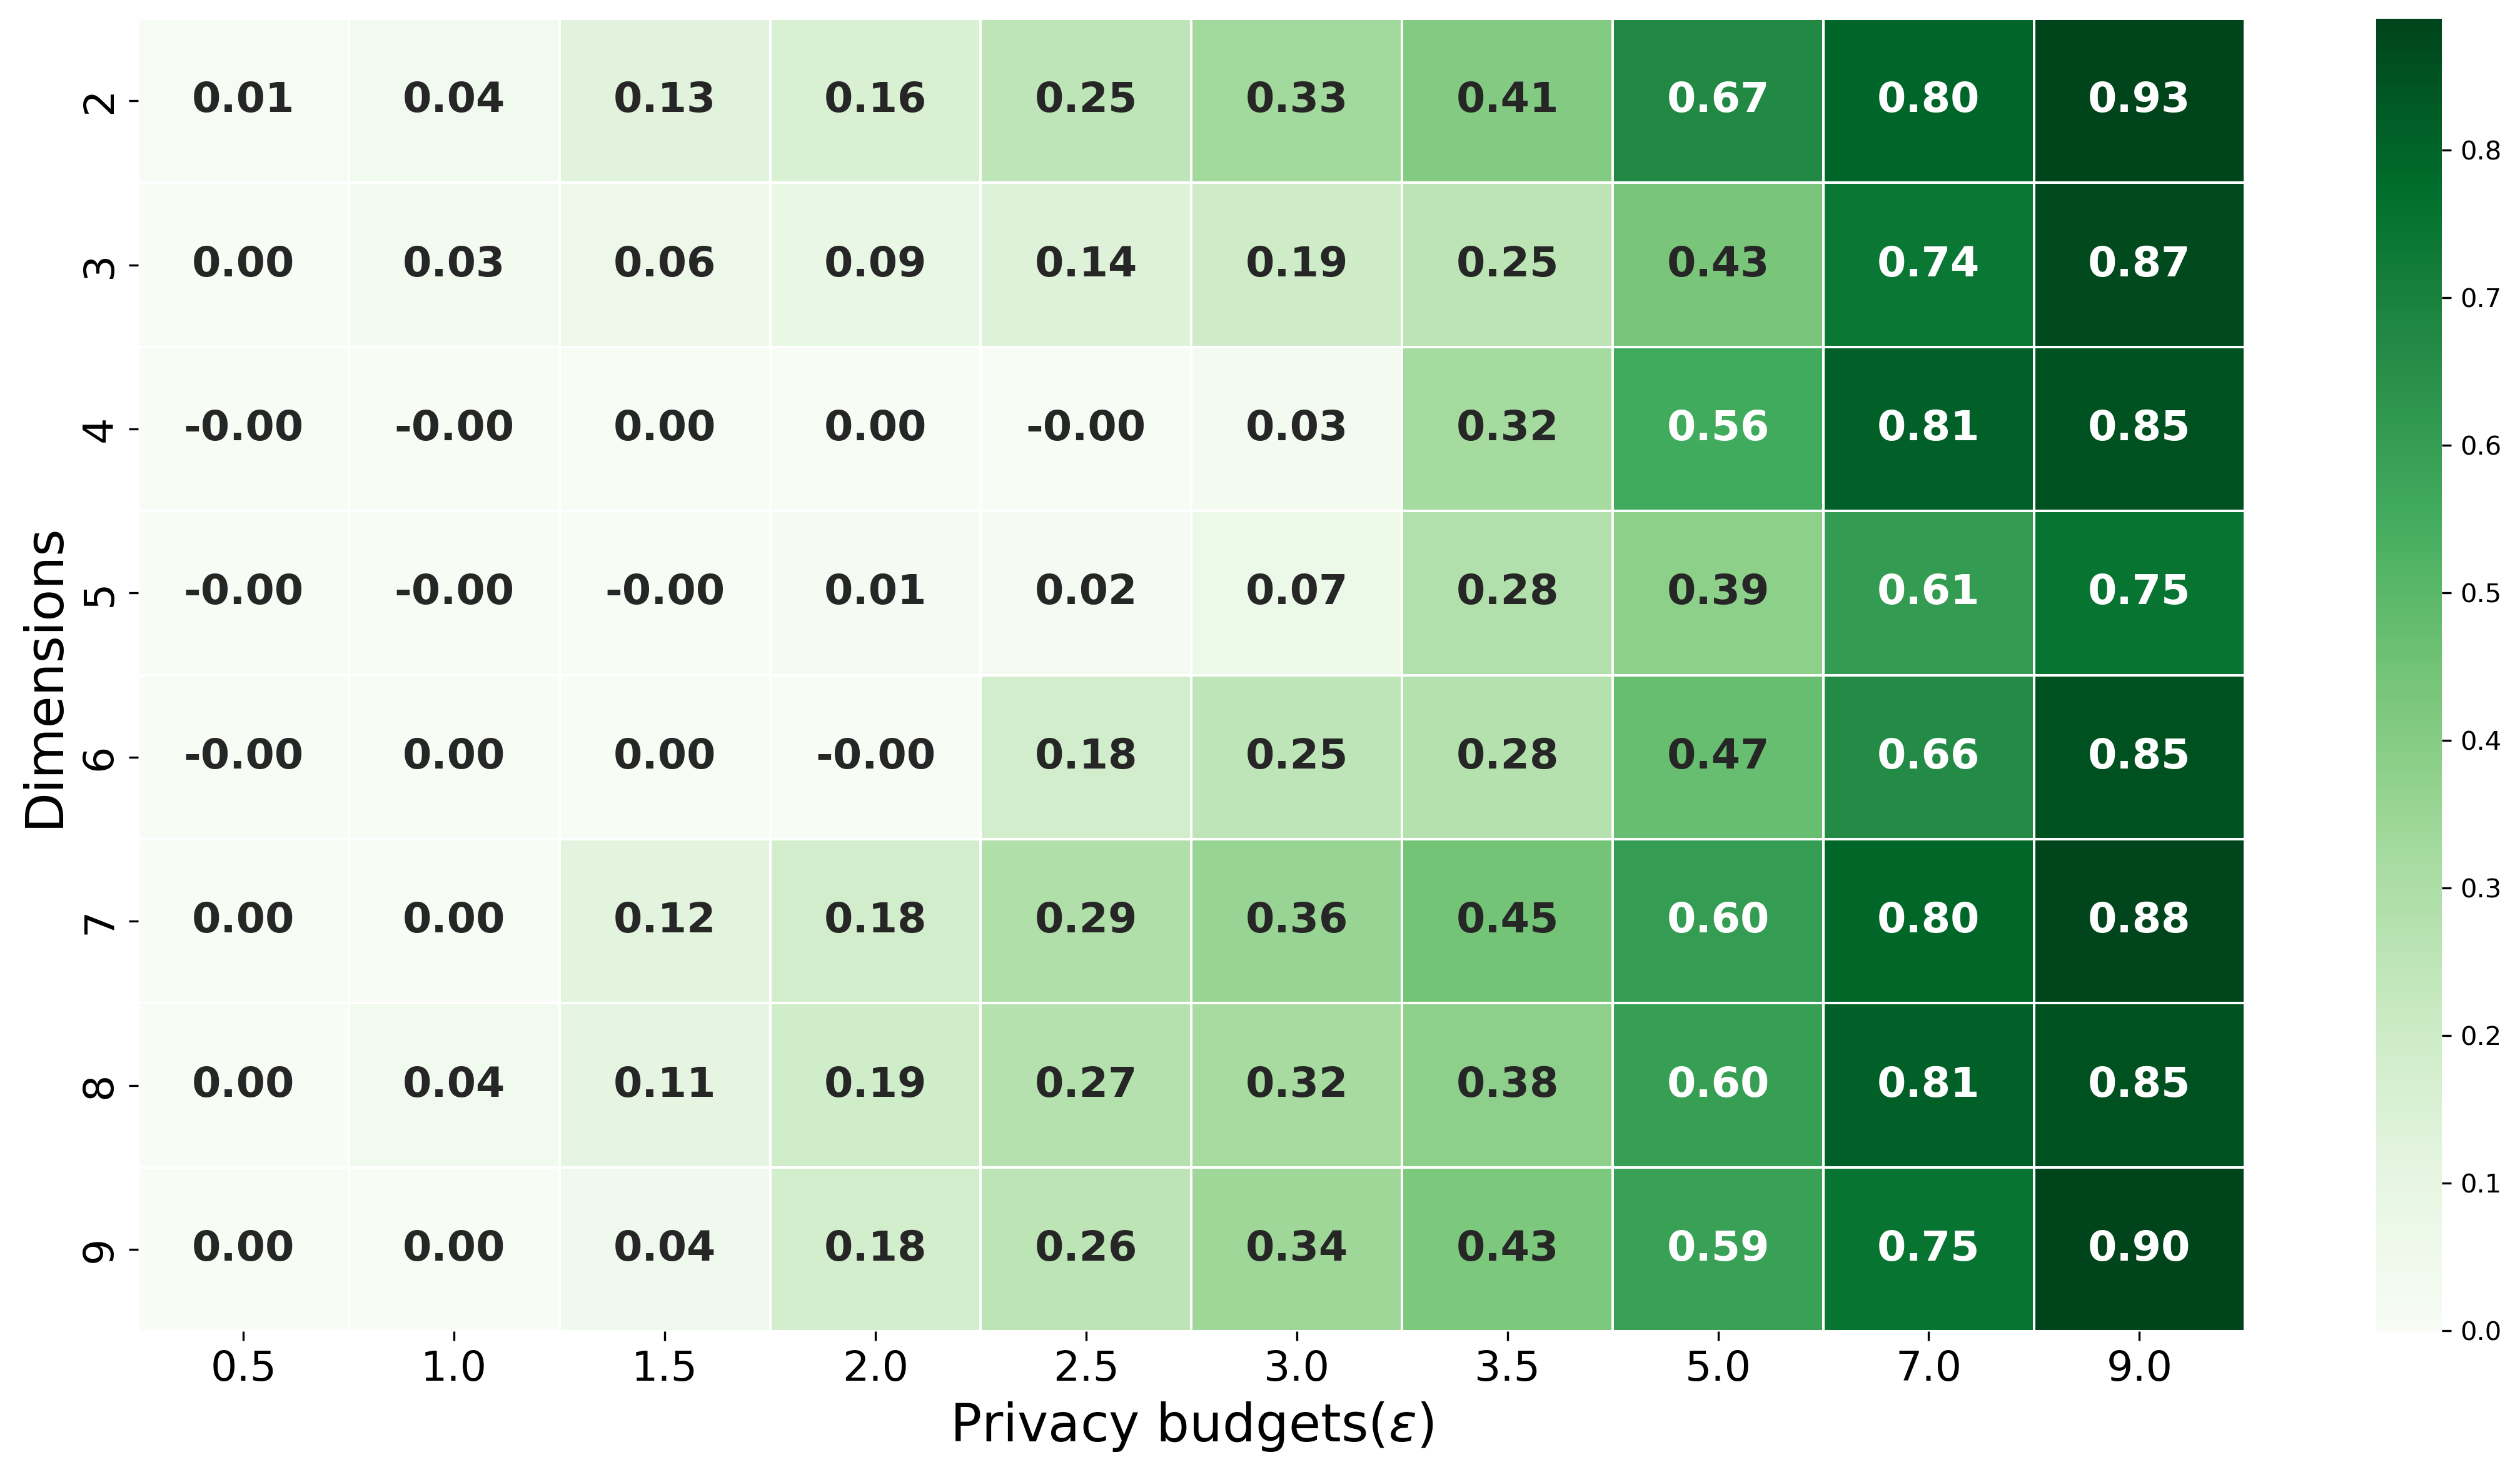
\includegraphics[width=1\textwidth]{Results/nd-laplace/piecewise/heart-dataset/ami.png}
      \label{fig:ami_heart-dataset_comparison_piecewise_2d}
    \end{subfigure}
  \end{subfigure}
\end{figure}
The scores for the heart-dataset are, as expected, in favor of nD-Laplace. We observe the same trend as in the cluster analysis, where nD-Laplace performs well across almost all privacy budgets. The performance of the 3D-Laplace implementation is slightly inferior, a finding that was also noted for the seeds-dataset. The influence of dimensions appears to be somewhat less pronounced than in the seeds-dataset, but from the 5th dimension onward, its impact becomes more significant.

The Piecewise mechanism scores low for privacy budgets between 0.5 and 3. Notably, the scores for 4 and 5 dimensions are considerably lower for these privacy budgets. Beyond that, the number of dimensions has minimal influence on the outcomes, with the privacy budget being the primary determinant.
\todo[inline]{Why are the 4 / 5 dimensions worse?}
\newpage
\mycomment{
\subsection{Circle-dataset}
\begin{figure}[H]
  \centering
  \begin{subfigure}[b]{0.8\textwidth}
    \begin{subfigure}[c]{1\textwidth}
      \caption{\textbf{Adjusted Mutual Information comparison for the kd-Laplace mechanism}}
      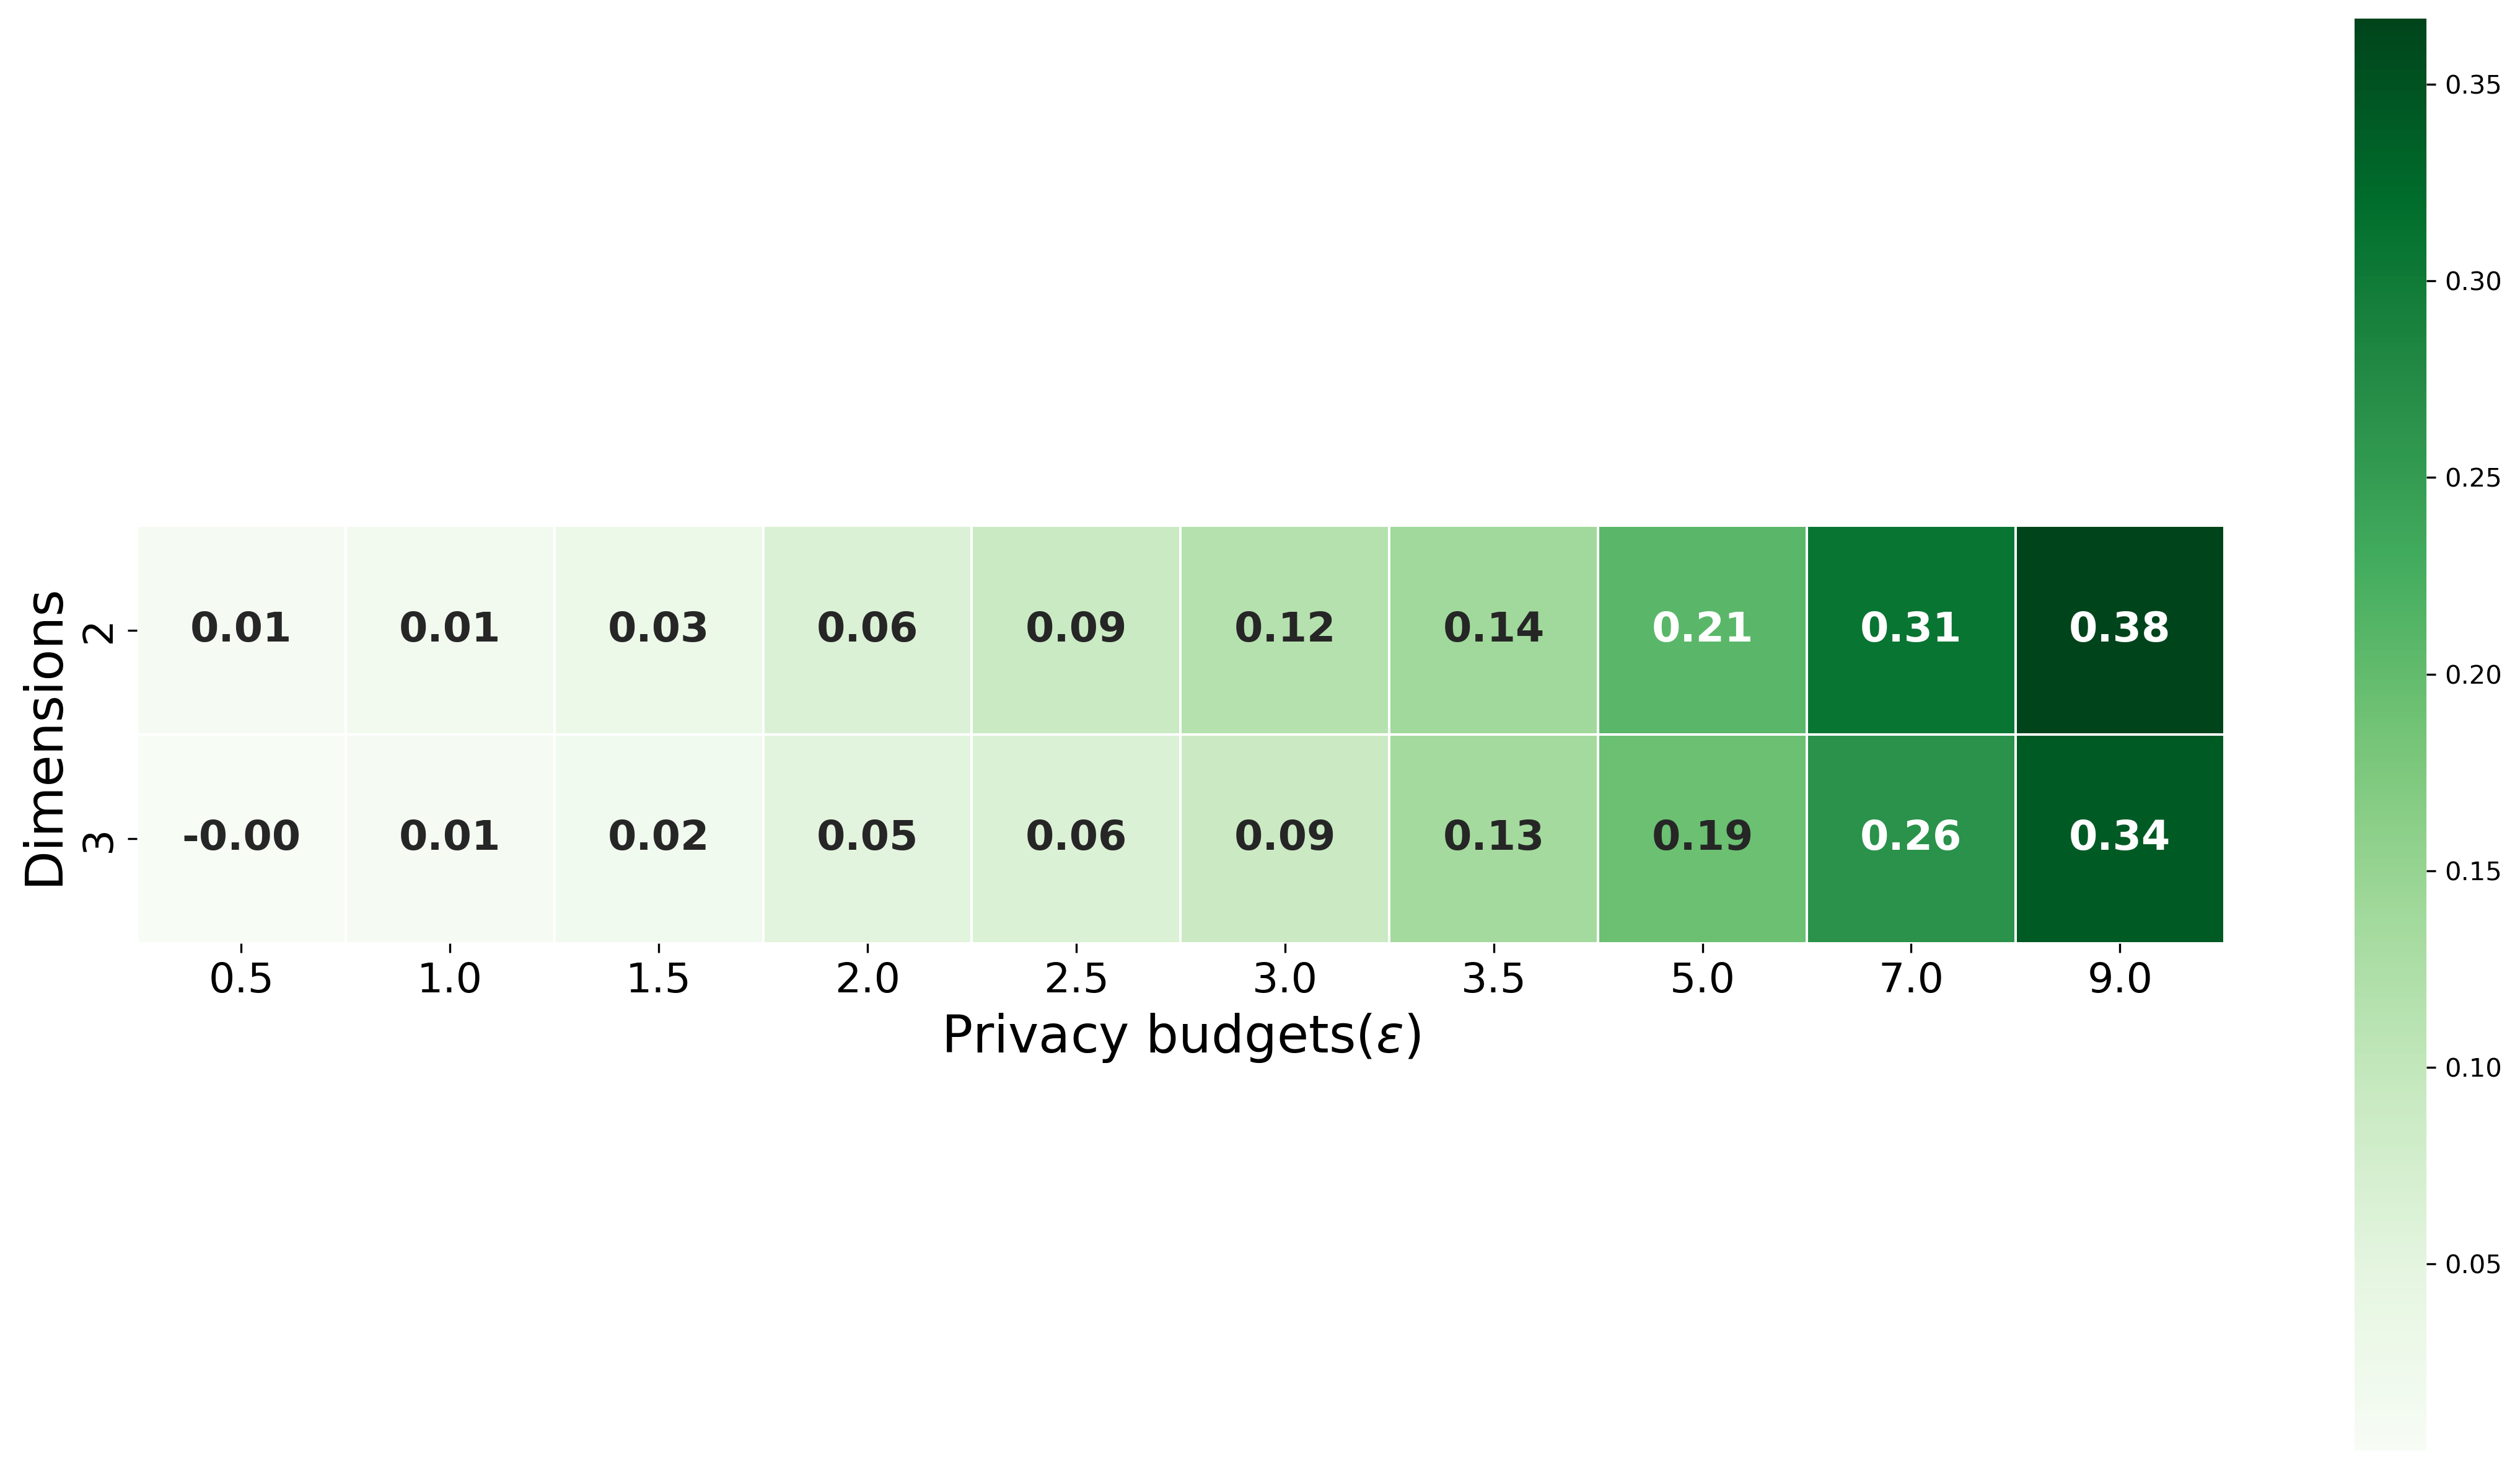
\includegraphics[width=1\textwidth]{Results/nd-laplace/nd-Laplace/circle-dataset/ami.png}
      \label{fig:ami_circle-dataset_comparison_kdlaplace_2d}
    \end{subfigure}
    \vfill % vertical space
    \begin{subfigure}[c]{1\textwidth}
      \caption{\textbf{Adjusted Mutual Information comparison for the Piecewise mechanism}}
      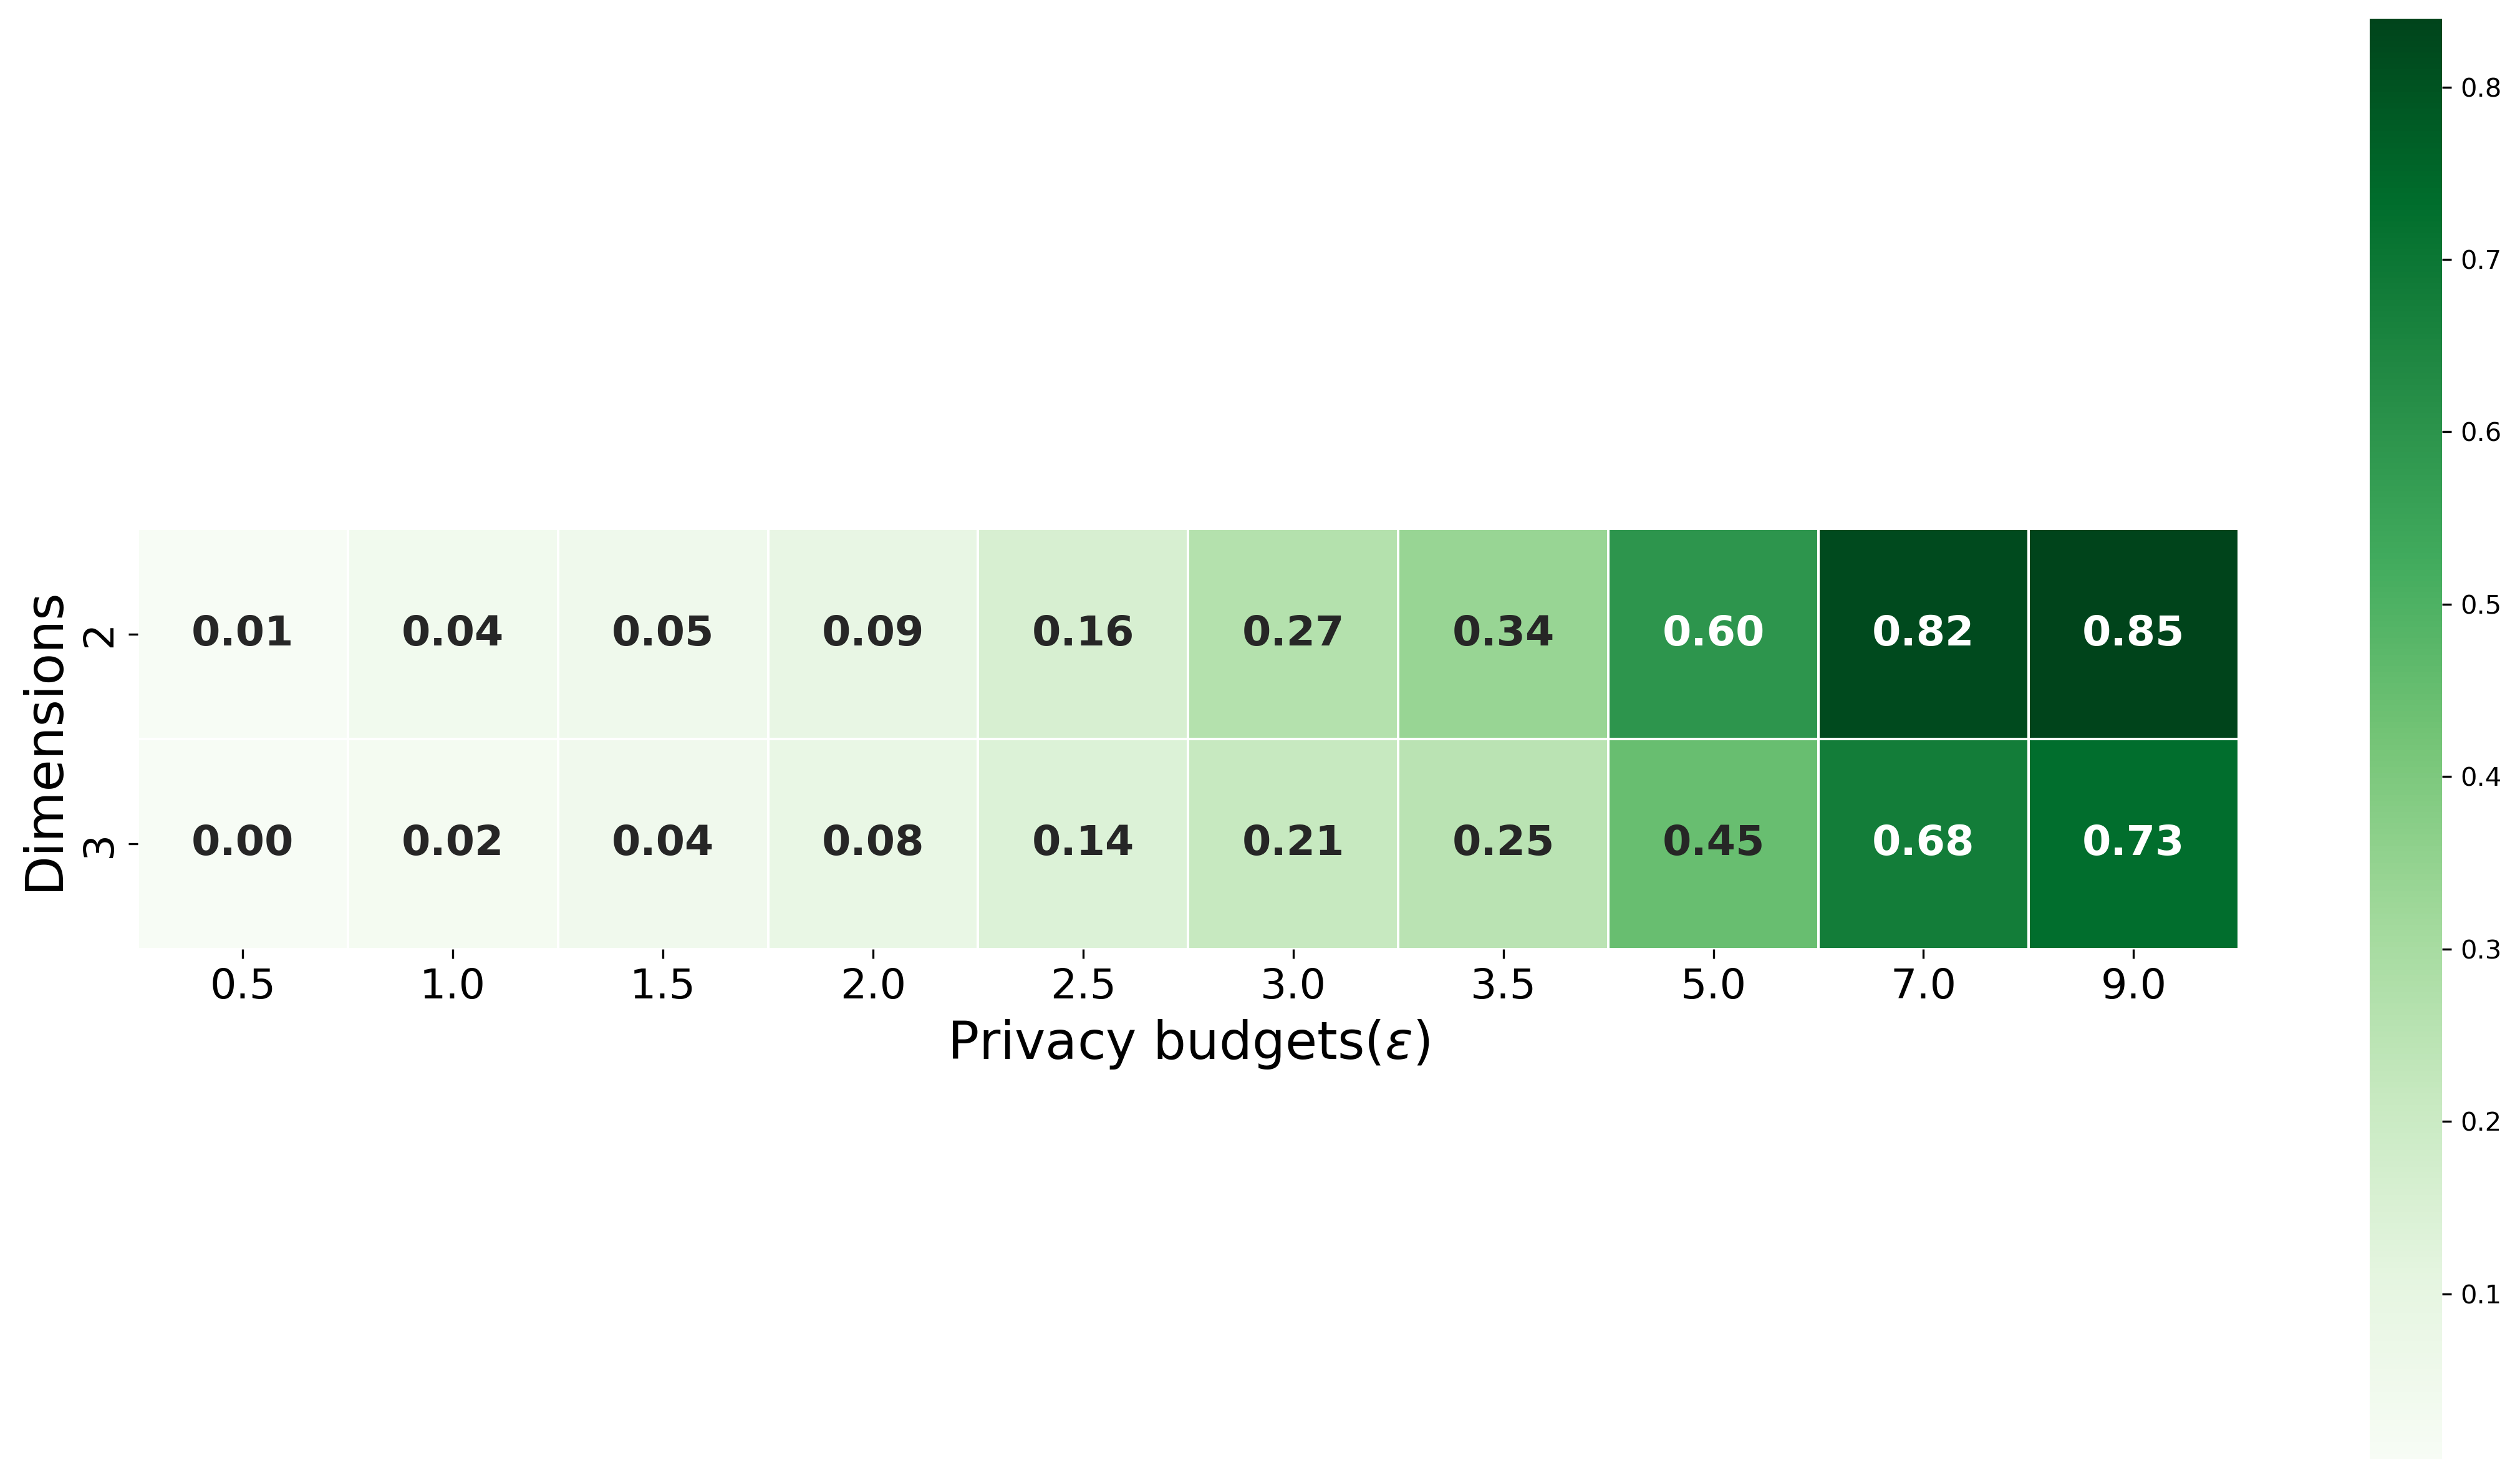
\includegraphics[width=1\textwidth]{Results/nd-laplace/piecewise/circle-dataset/ami.png}
      \label{fig:ami_circle-dataset_comparison_piecewise_2d}
    \end{subfigure}
  \end{subfigure}
\end{figure}

\newpage
\subsection{Line-dataset}
\begin{figure}[H]
  \centering
  \begin{subfigure}[b]{0.85\textwidth}
    \begin{subfigure}[c]{1\textwidth}
      \caption{\textbf{Adjusted Mutual Information comparison for the kd-Laplace mechanism}}
      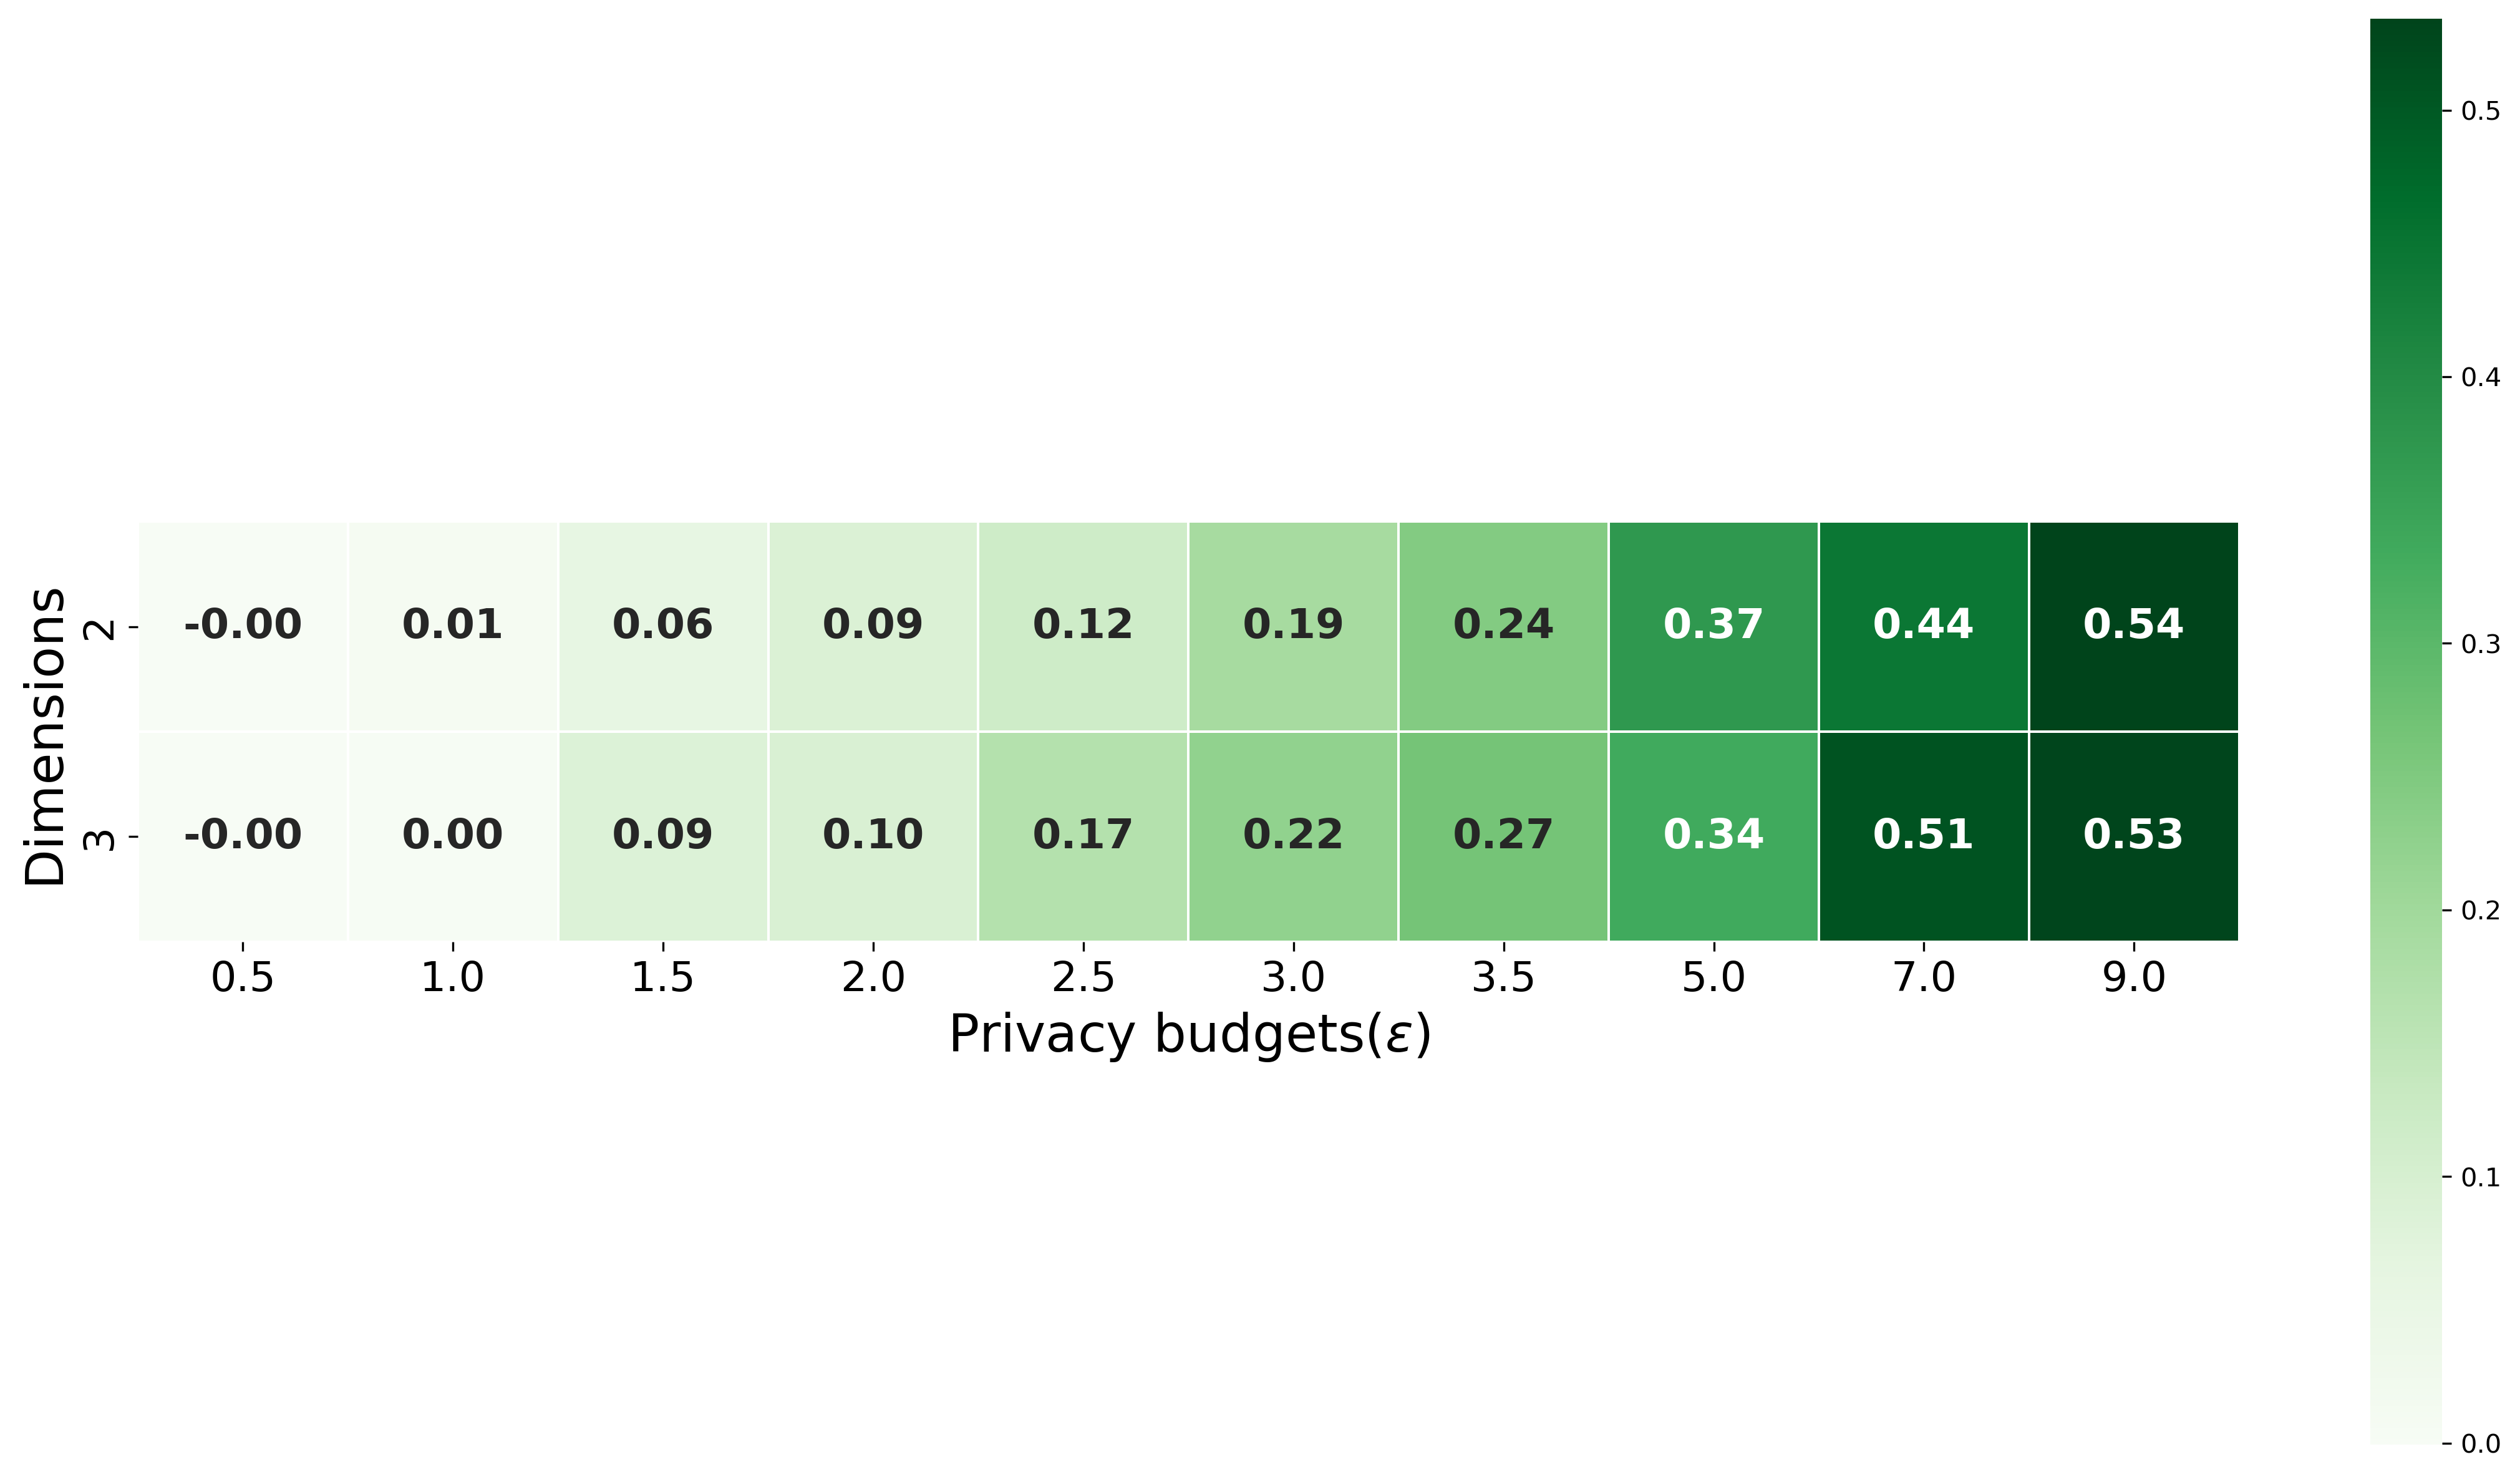
\includegraphics[width=1\textwidth]{Results/nd-laplace/nd-Laplace/line-dataset/ami.png}
      \label{fig:ami_line-dataset_comparison_kdlaplace_2d}
    \end{subfigure}
    \vfill % vertical space
    \begin{subfigure}[c]{1\textwidth}
      \caption{\textbf{Adjusted Mutual Information comparison for the Piecewise mechanism}}
      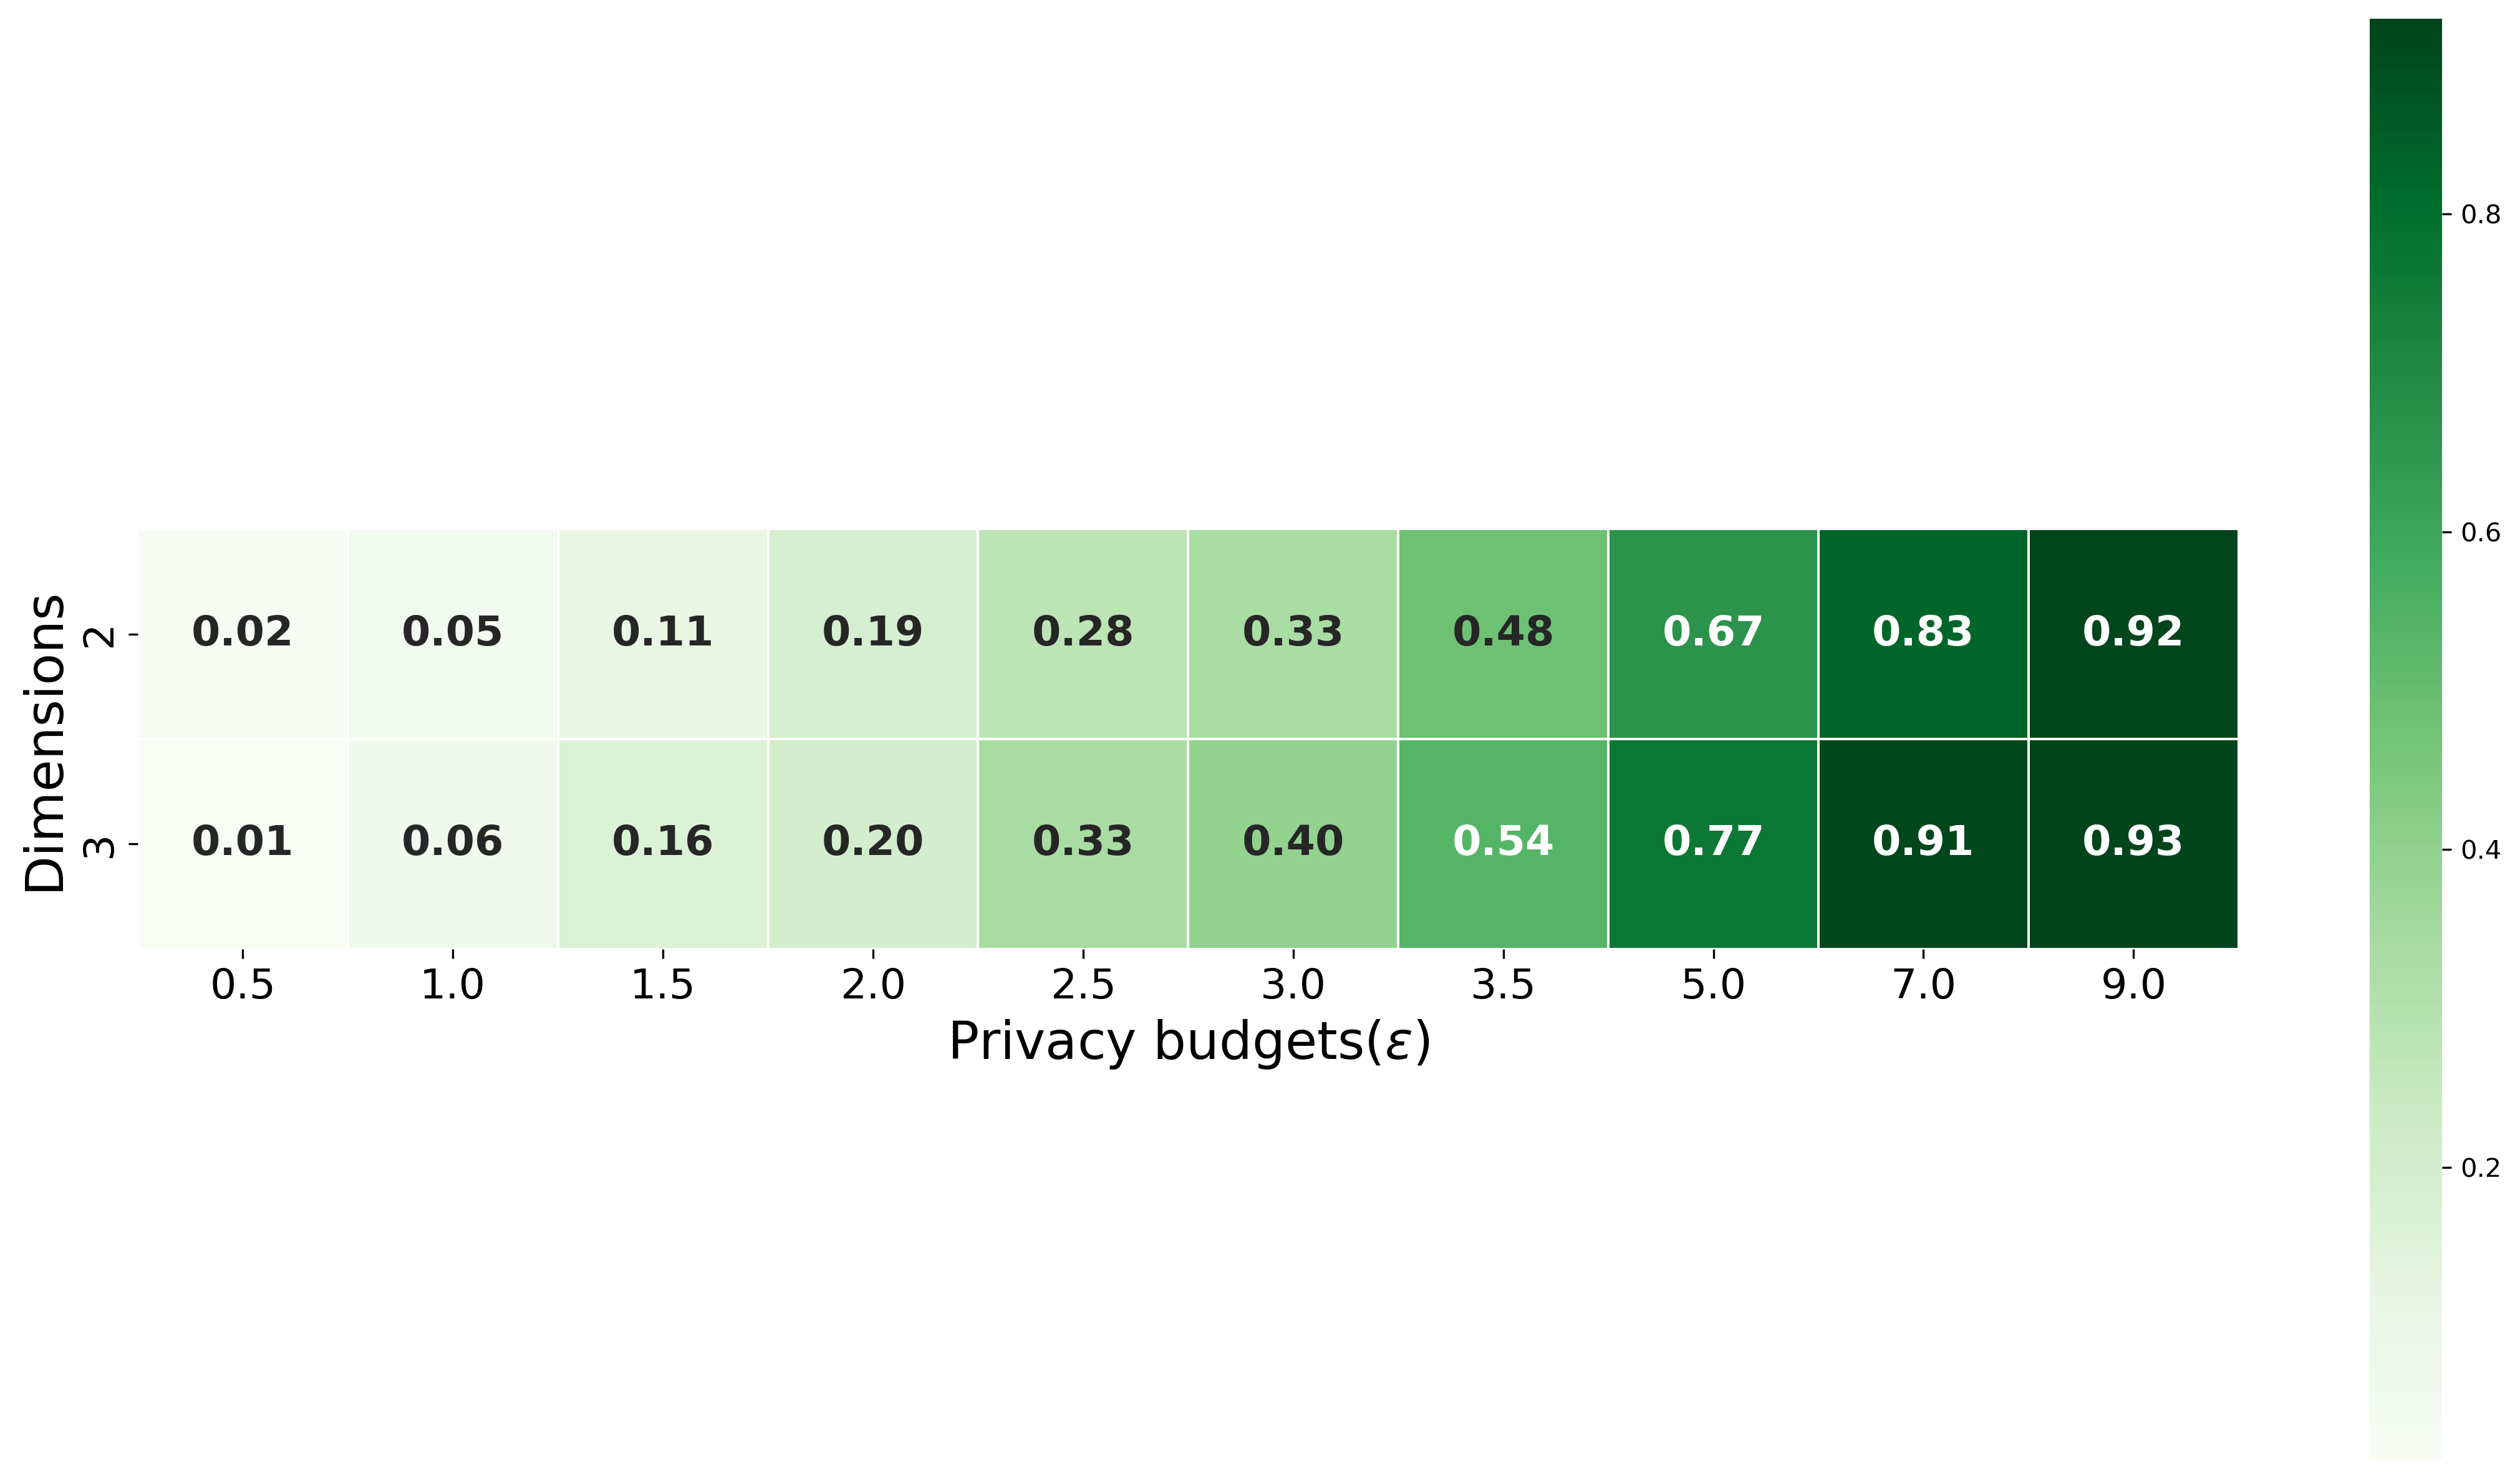
\includegraphics[width=1\textwidth]{Results/nd-laplace/piecewise/line-dataset/ami.png}
      \label{fig:ami_line-dataset_comparison_piecewise_2d}
    \end{subfigure}
  \end{subfigure}
\end{figure}
Up to privacy budget 3.5, the scores remain relatively similar for both mechanisms, but after that, they become better for Piecewise.

For kD-Laplace, the highest score is 0.63 \gls{ami} for privacy budget 9. For privacy budgets 5 and 7, the score is around 0.5 - 0.55. After that, the scores are no higher than 0.37.

Piecewise performs better, with a maximum of 0.90 \gls{ami} for privacy budget 9 for 2 dimensions. For both mechanisms, the dimensions do not significantly impact the score.
\newpage
\subsection{Skewed-dataset}
\begin{figure}[H]
  \centering
  \begin{subfigure}[b]{0.85\textwidth}
    \begin{subfigure}[c]{1\textwidth}
      \caption{\textbf{Adjusted Mutual Information comparison for the kd-Laplace mechanism}}
      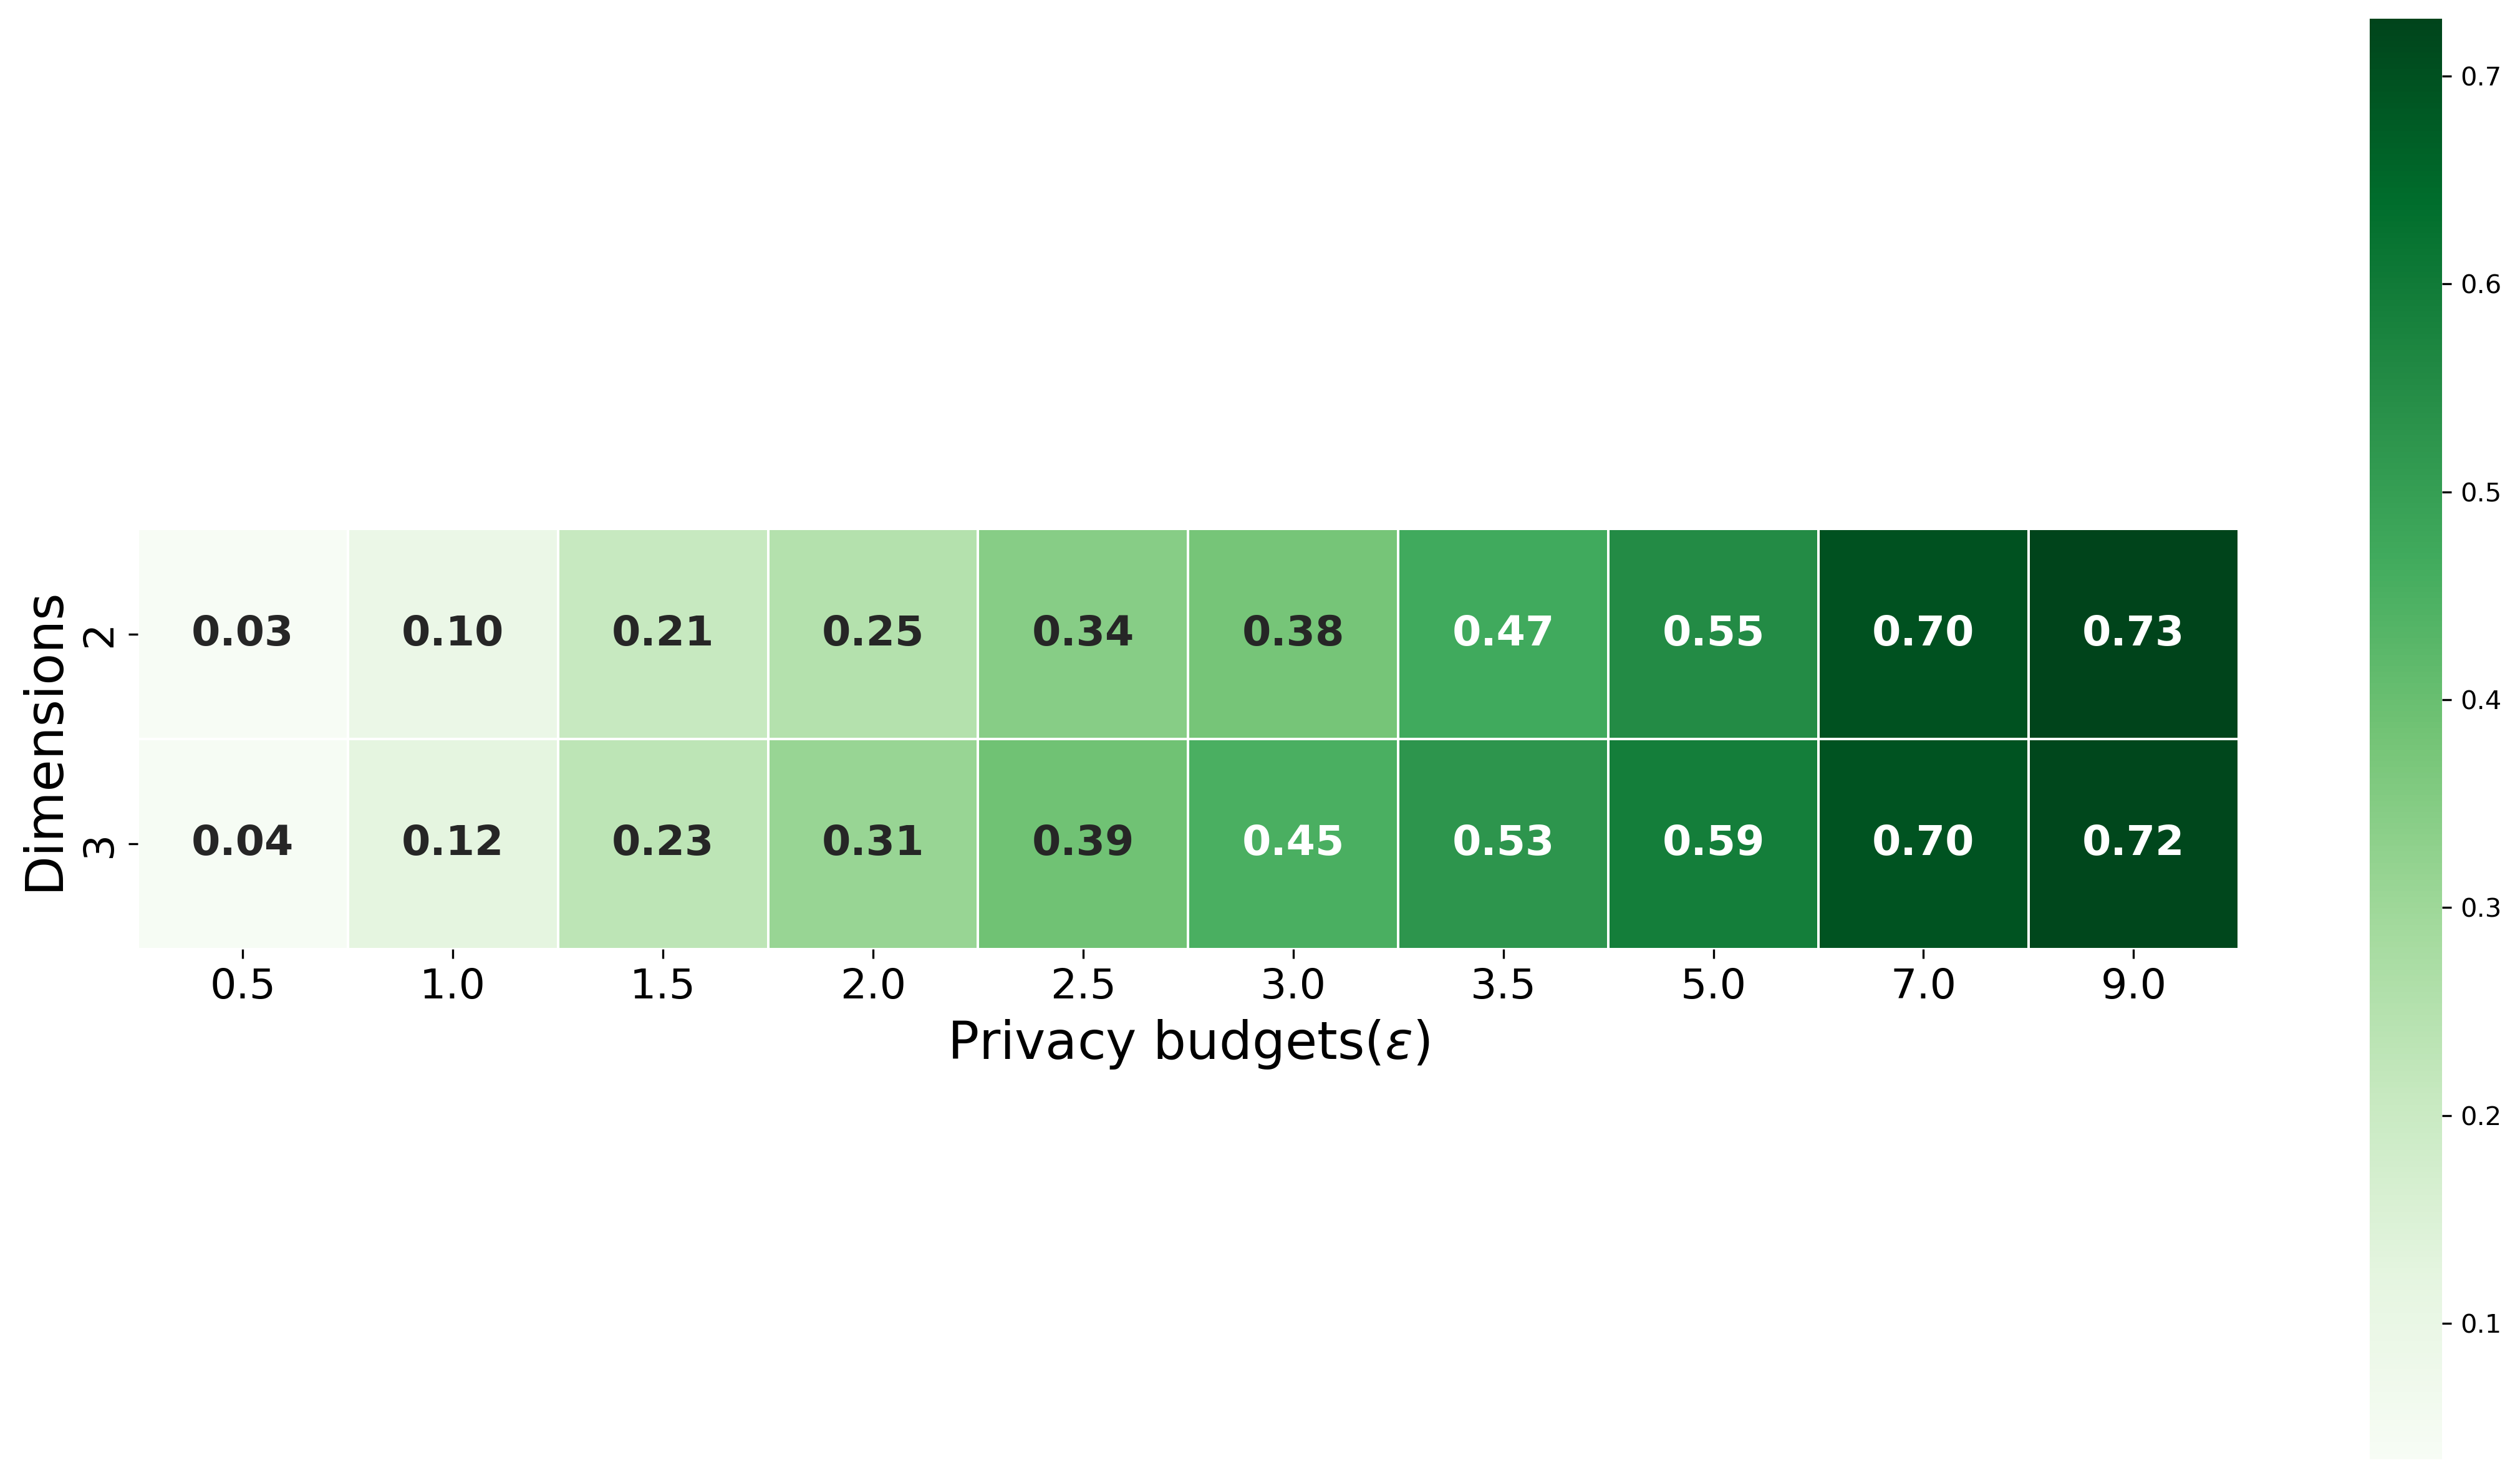
\includegraphics[width=1\textwidth]{Results/nd-laplace/nd-Laplace/skewed-dataset/ami.png}
      \label{fig:ami_skewed-dataset_comparison_kdlaplace_2d}
    \end{subfigure}
    \vfill % vertical space
    \begin{subfigure}[c]{1\textwidth}
      \caption{\textbf{Adjusted Mutual Information comparison for the Piecewise mechanism}}
      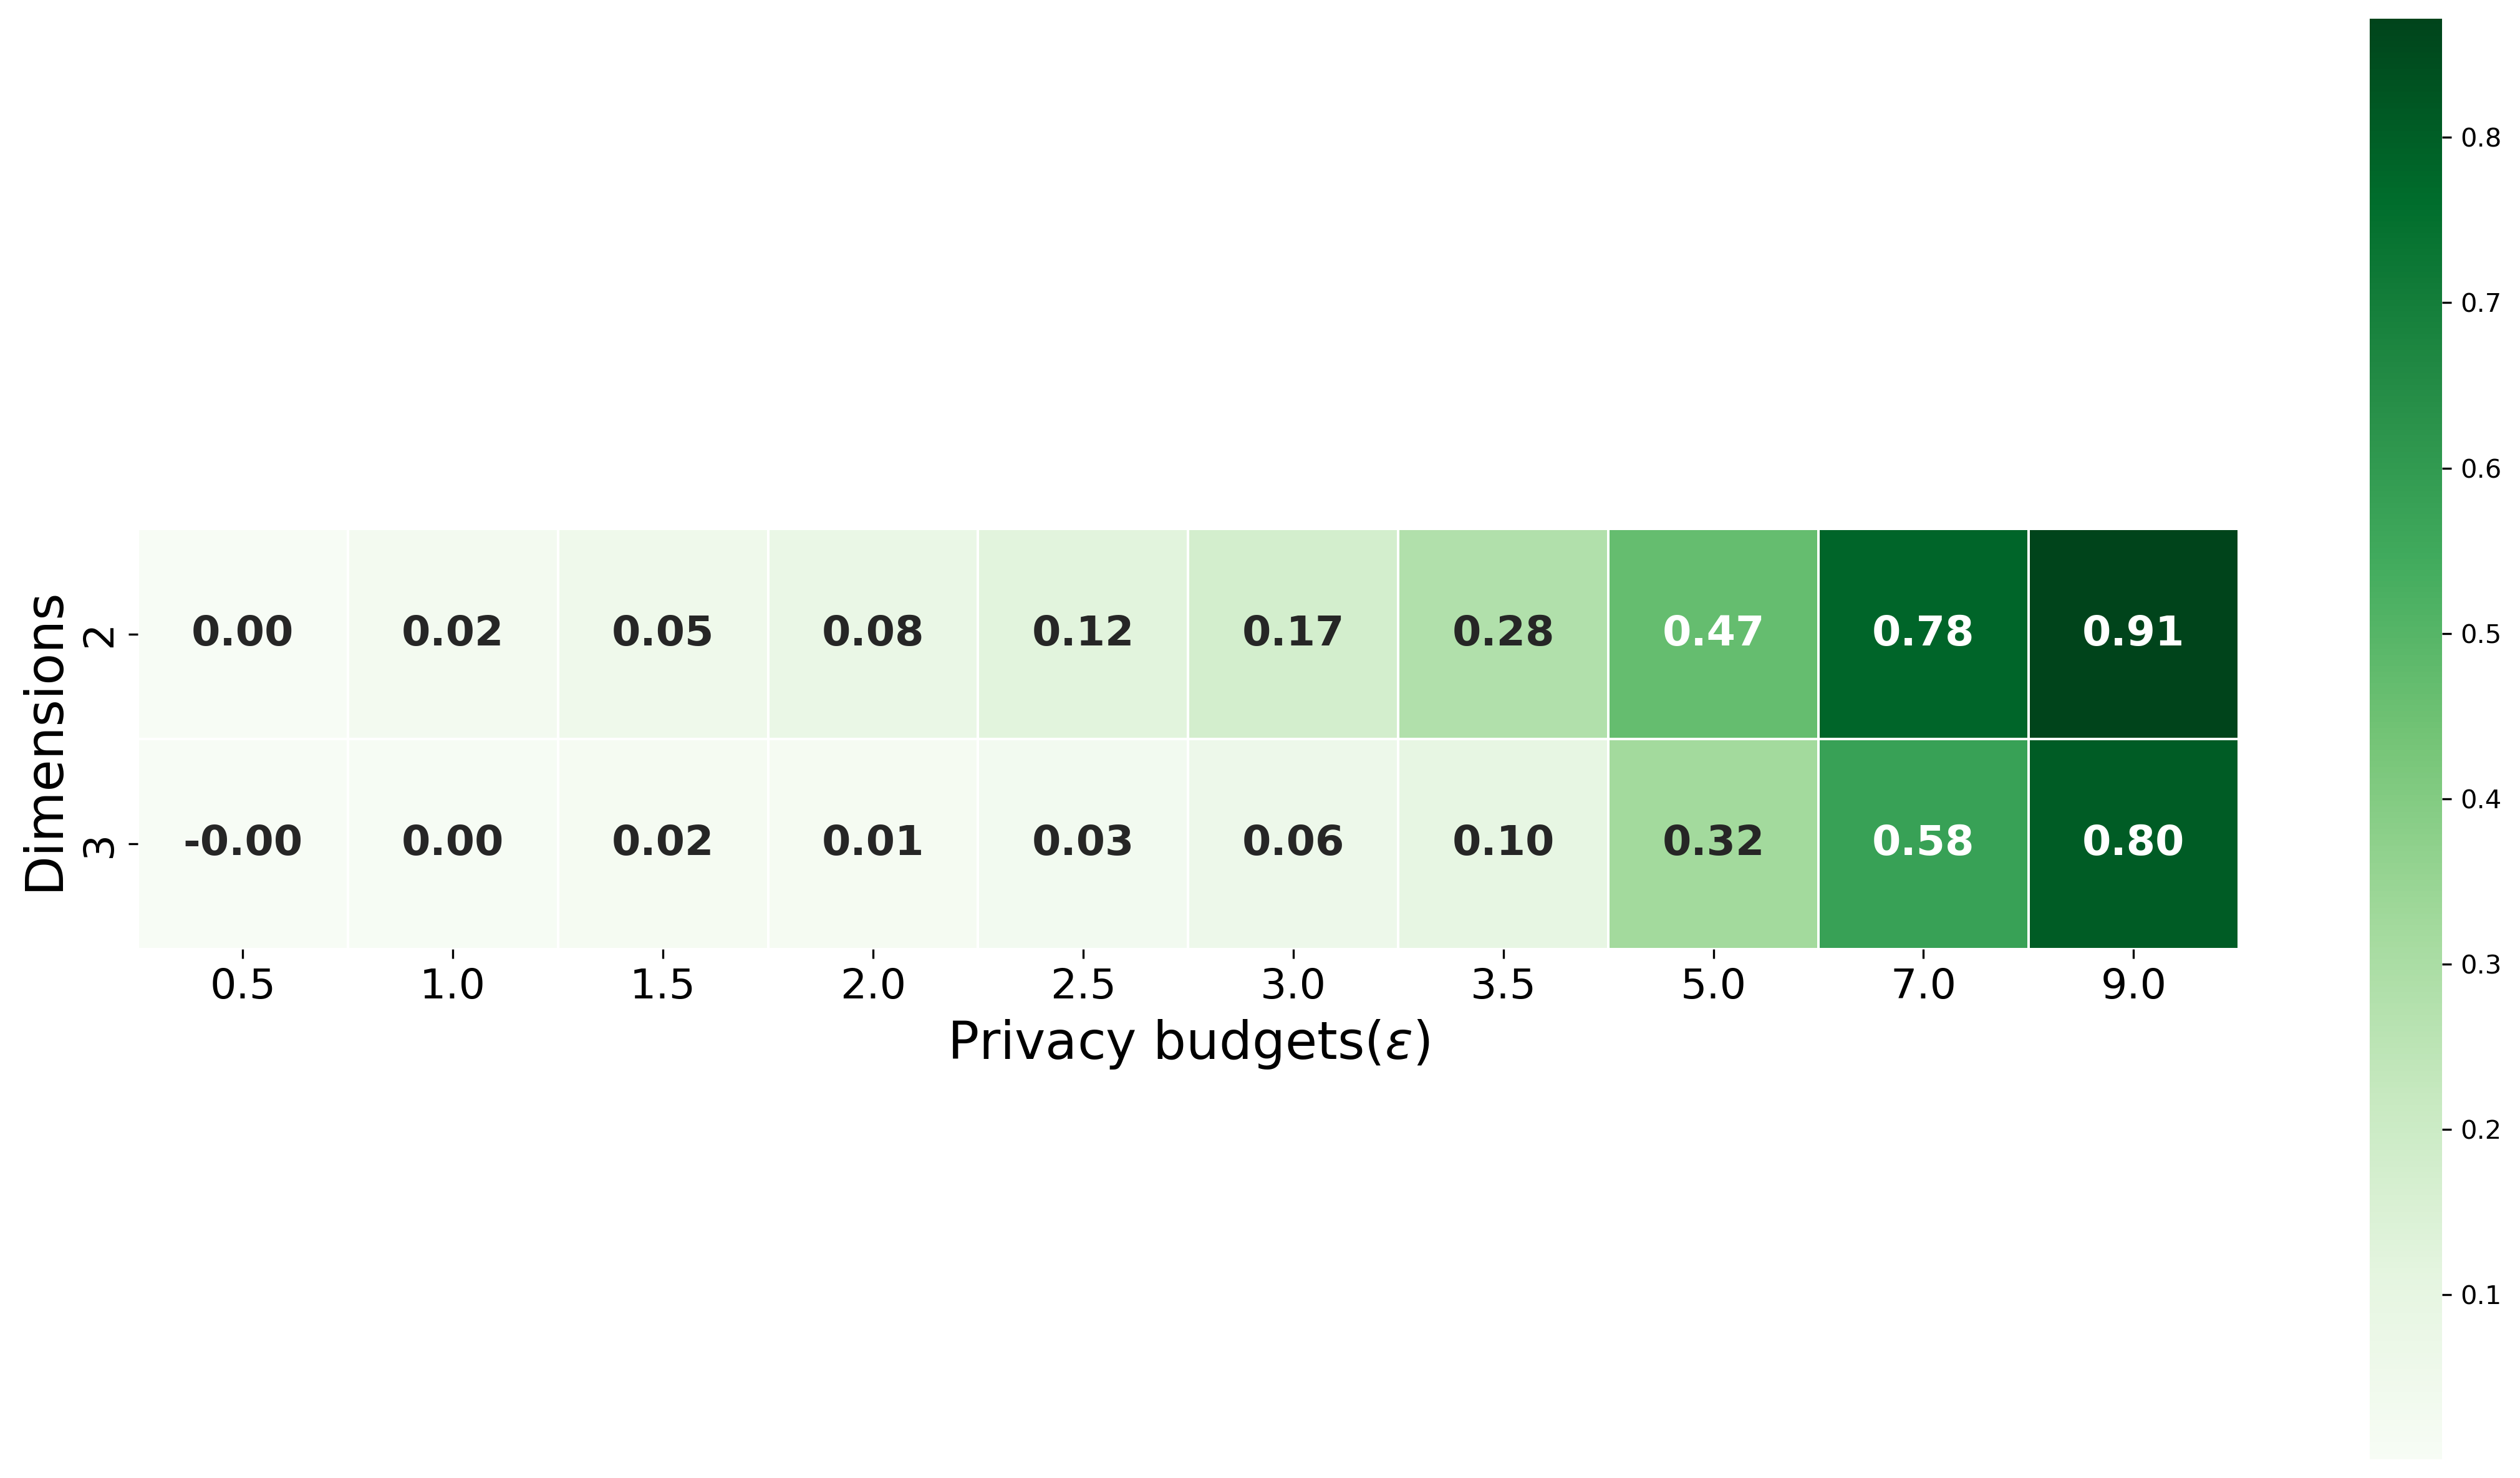
\includegraphics[width=1\textwidth]{Results/nd-laplace/piecewise/skewed-dataset/ami.png}
      \label{fig:ami_skewed-dataset_comparison_piecewise_2d}
    \end{subfigure}
  \end{subfigure}
\end{figure}
The kD-Laplace mechanism performs slightly better from privacy budgets 2 to 5. However, Piecewise performs significantly better after that, achieving around 0.73 and 0.85 \gls{ami} for privacy budgets 7 and 9, respectively.

In contrast, kD-Laplace scores much lower in this range. Furthermore, it appears that the dimensions do not significantly impact the performance of the mechanisms in this context.
\newpage
}

\section{Privacy}
The sections below present a heatmap comparison of the nd-Laplace and Piecewise mechanisms.
We employed a heatmap to simultaneously depict the privacy budget (epsilon), the number of dimensions, and a specific metric. The metrics we use for this are the Membership advantage, \gls{tpr} and privacy distance. 

On the heatmap, the x-axis represents the privacy budget, while the y-axis illustrates the number of dimensions. Each cell of the heatmap displays the specific metric value. The intensity of the cell's color corresponds to the \gls{ami} score: a darker shade signifies a higher score:
\begin{enumerate}
    \item  For the membership advantage and \gls{tpr}, a lighter cell color (lower value) indicates a better score.
    \item For the privacy distance, the opposite is true; if the cell color is dark (high value), it provides more distance and thus more privacy.
\end{enumerate}
%The images below display bar plots for the membership advantage and TPR of membership inference attacks as described in the methodology.
%We use the same color scheme in the previous section to display the different mechanisms.
%In addition, a red line was drawn to indicate the baseline TPR (the non-private dataset's TPR). \newline
\newpage
\subsection{Seeds dataset}
\begin{figure}[H]
  \centering
  \begin{subfigure}[b]{0.75\textwidth}
    \begin{subfigure}[c]{1\textwidth}
      \caption{\textbf{Heatmap showing adversary advantage for the kD-Laplace mechanism, per privacy budget \& dimension for seeds-dataset.}}
      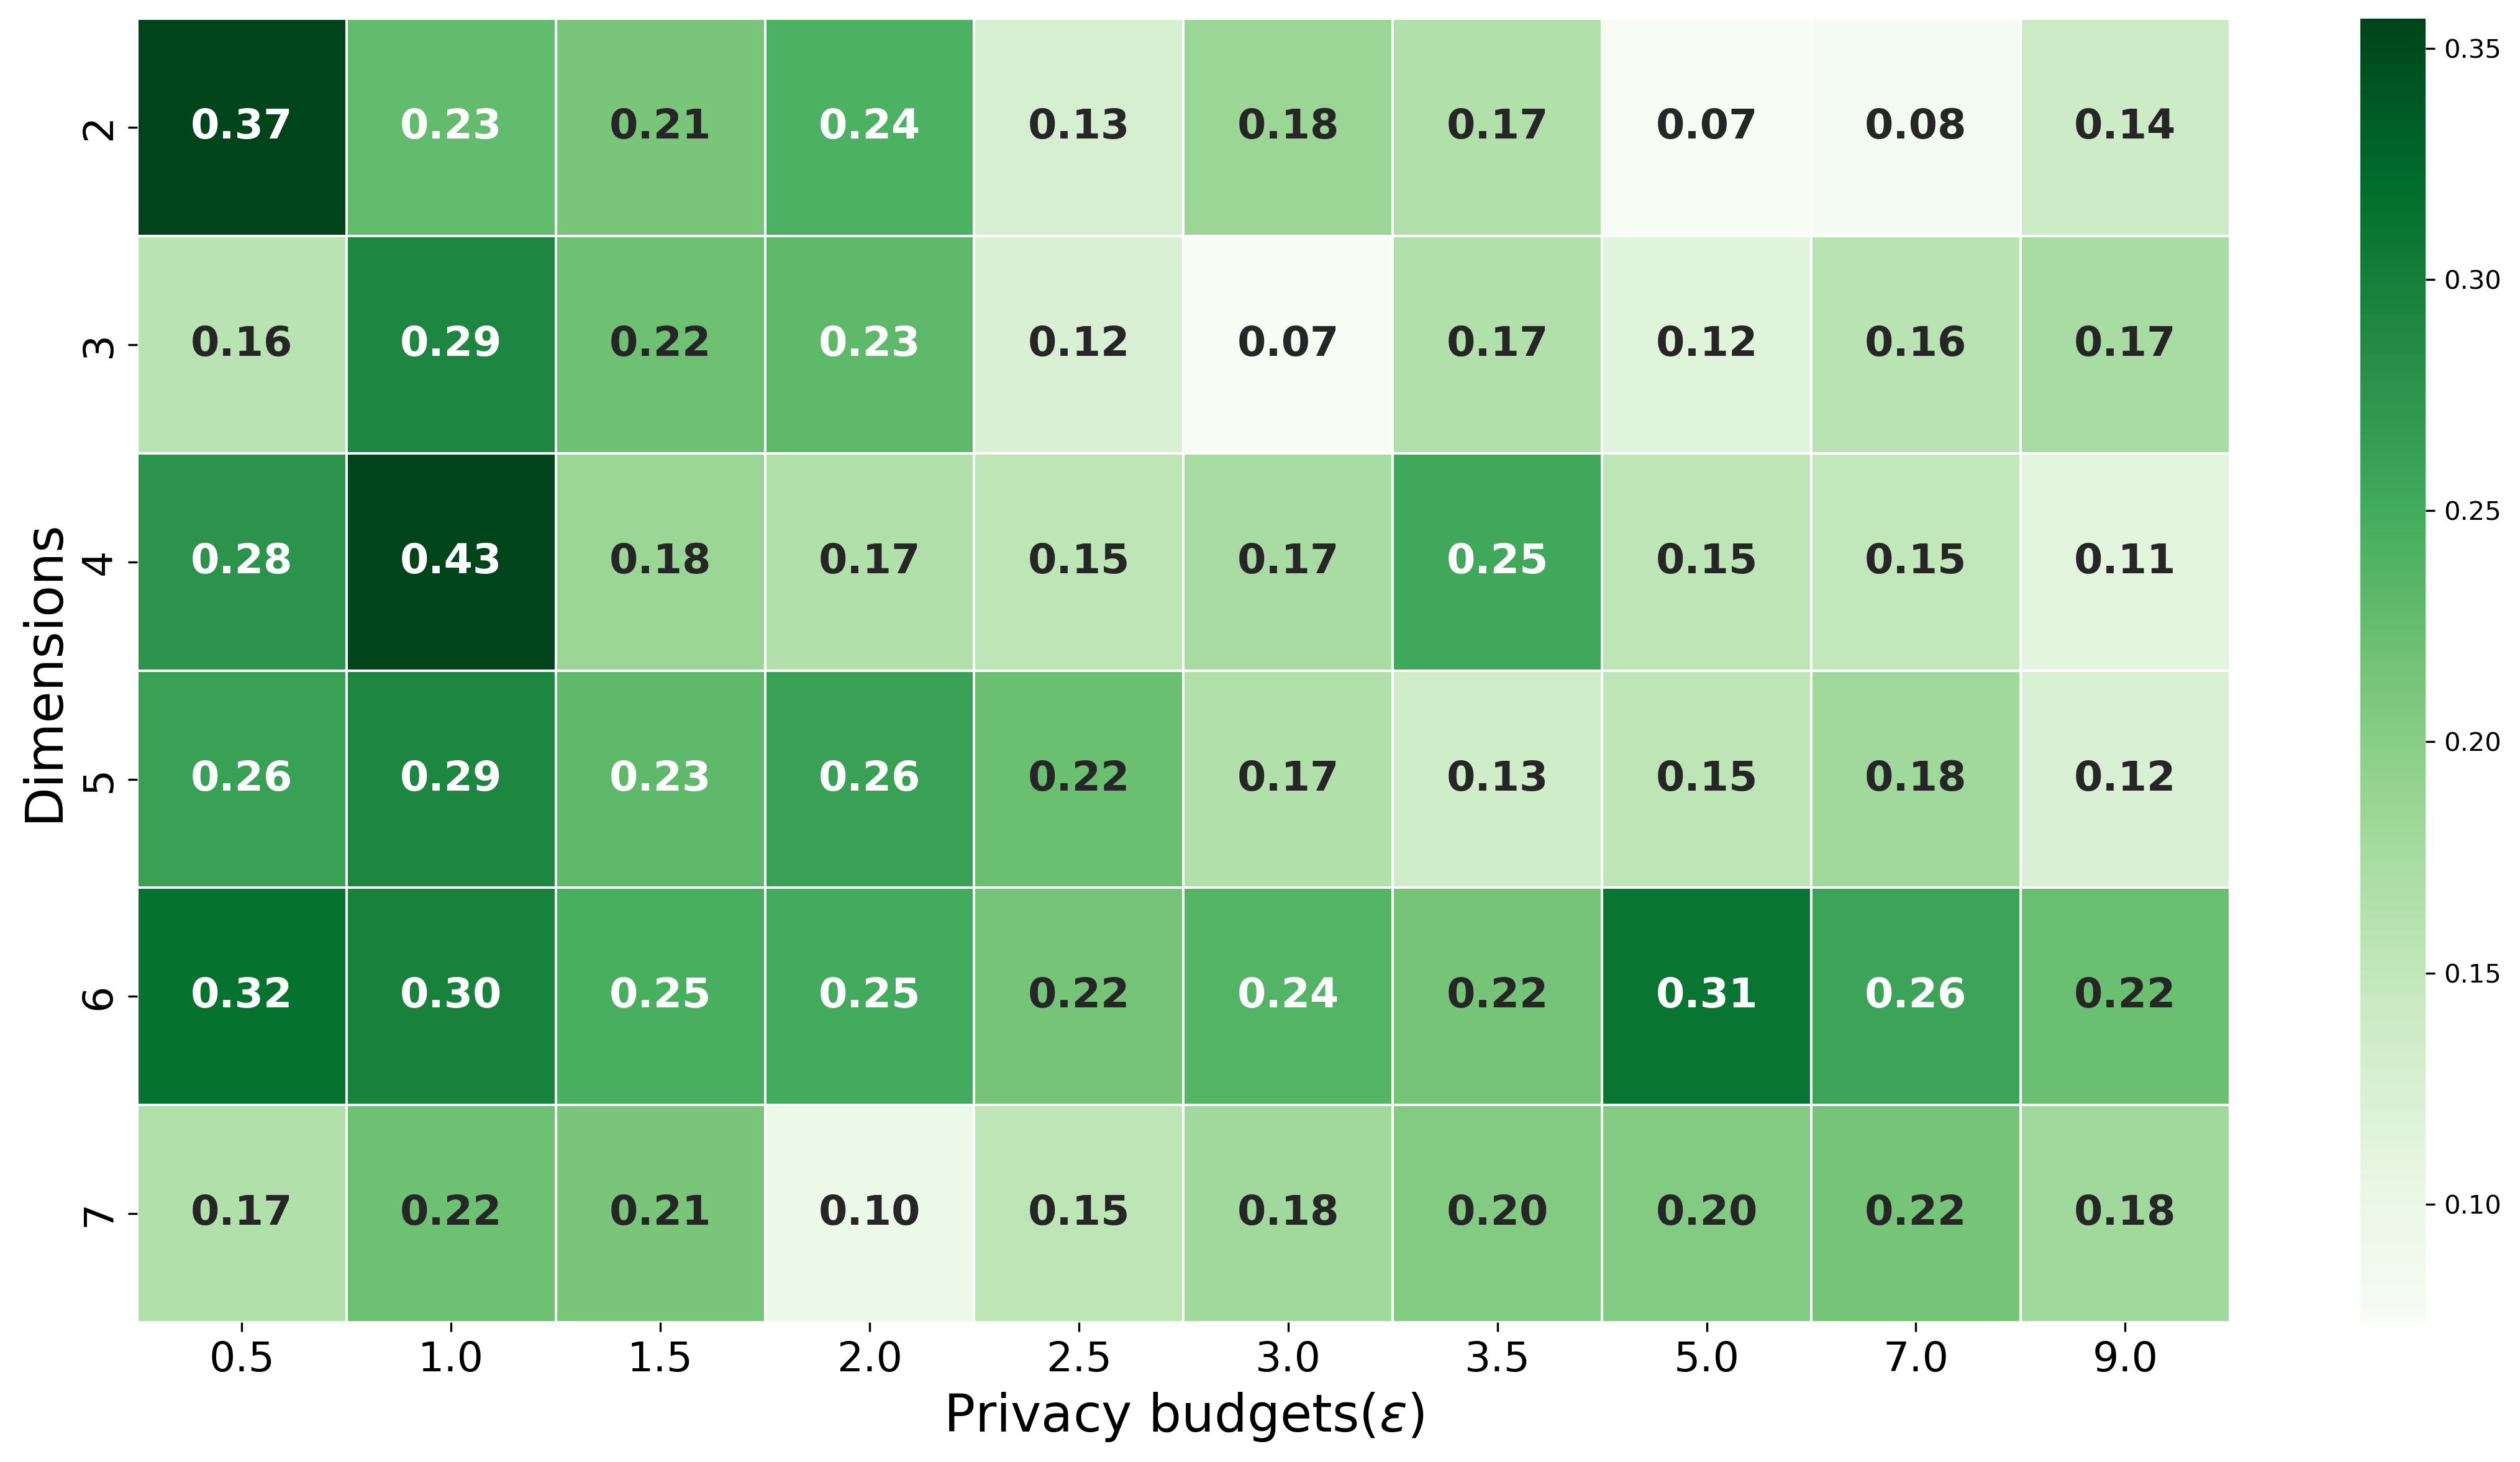
\includegraphics[width=1\textwidth]{Results/nd-laplace/nd-Laplace/seeds-dataset/shokri_mi_adv.png}
      \label{fig:privacy_seeds-dataset_adversial_advantage_kd-laplace}
    \end{subfigure}
    \vfill % vertical space

    \begin{subfigure}[c]{1\textwidth}
      \caption{\textbf{Heatmap showing adversary advantage for the Piecewise mechanism, per privacy budget \& dimension for seeds-dataset.}}
      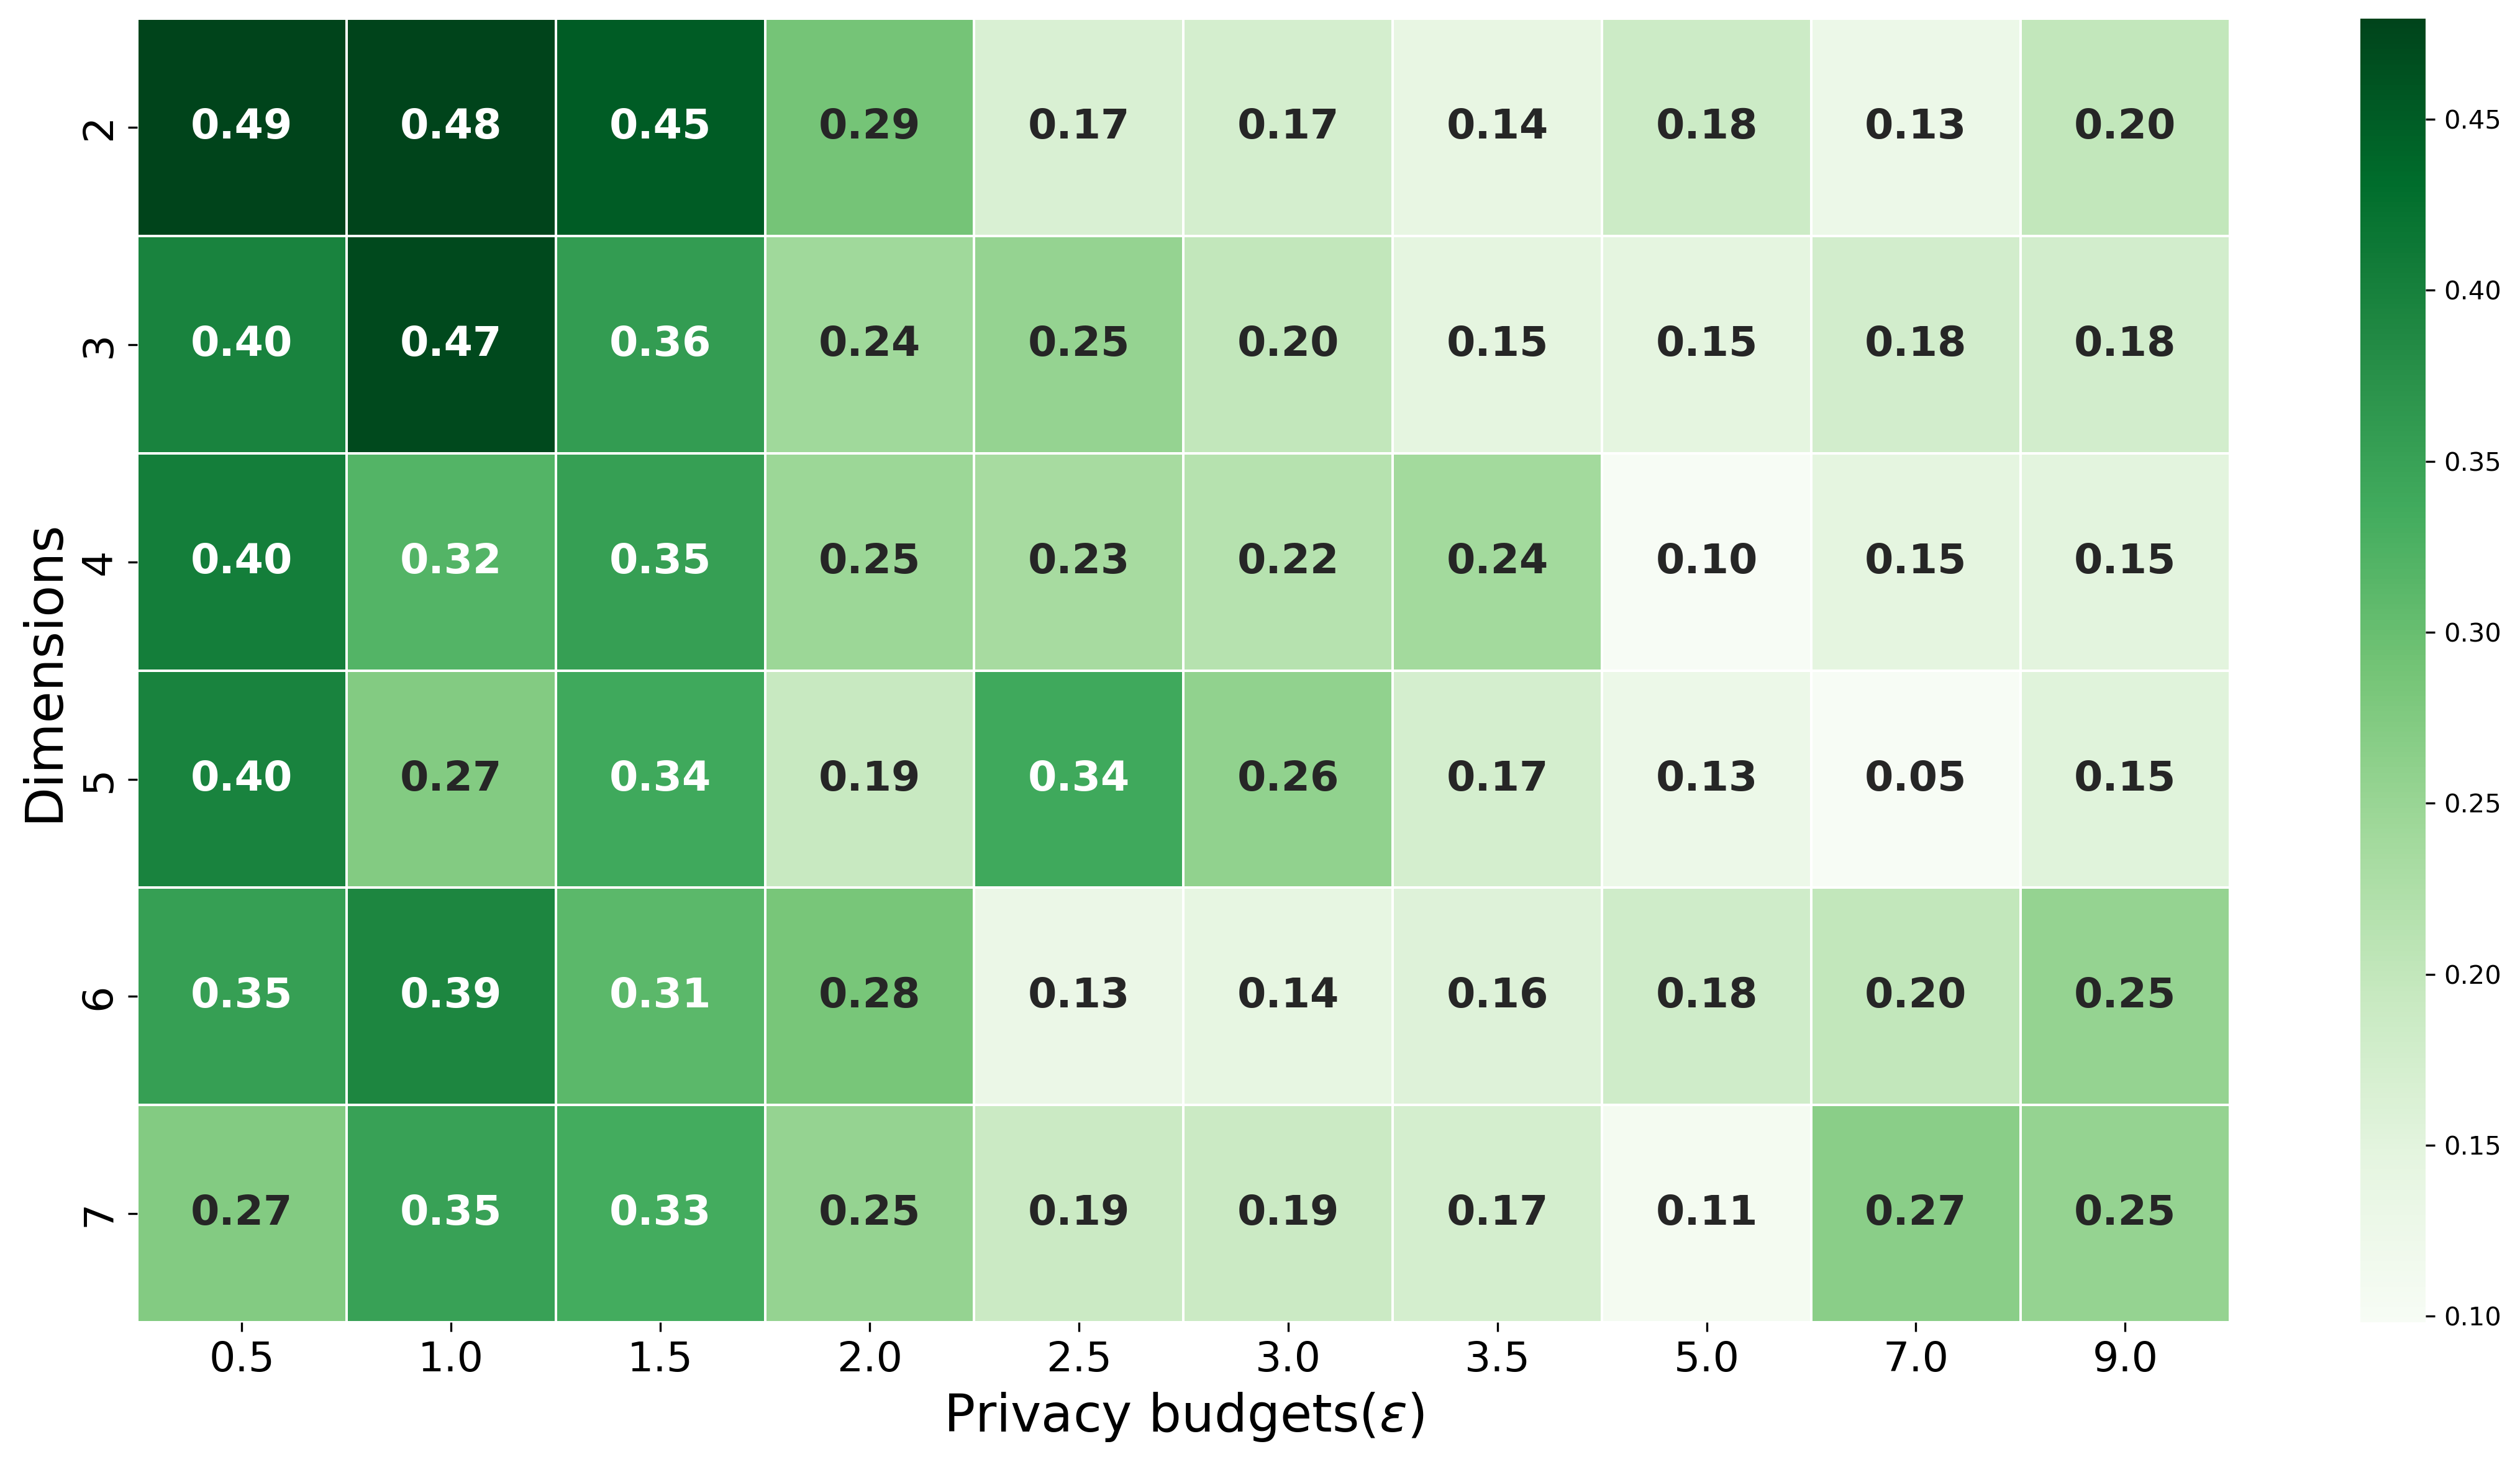
\includegraphics[width=1\textwidth]{Results/nd-laplace/piecewise/seeds-dataset/shokri_mi_adv.png}
      \label{fig:privacy_seeds-dataset_adversial_advantage_piecewise}
    \end{subfigure}
  \end{subfigure}
\end{figure}
When comparing the mechanisms, we observe that nD-Laplace has a relatively high score for epsilon values ranging from 0.5 to 2.5. The dimensions also seem to influence this, as dimensions 6 and 7 appear slightly darker. As the privacy budgets increase, the adversary advantage decreases. This trend is also evident in the Piecewise mechanism. The number of dimensions doesn't have much influence, but it's clear that for epsilons 0.5 to 1.5, the dimensional data has a higher adversary advantage.

We would expect the adversary advantage increasing from left to right, because a higher privacy budget indicates low noise. So, the \gls{mia} should be higher.
To get a clearer picture why this is not happing, we consider the \gls{tpr}, which represents the accurately retrieved information (See next page). \newpage
\begin{figure}[H]
    \centering
    \begin{subfigure}[b]{0.75\textwidth}
        \begin{subfigure}[c]{1\textwidth}
            \caption{\textbf{Heatmap TPR for the kD-Laplace mechanism, per privacy budget \& dimension for seeds-dataset.}}
            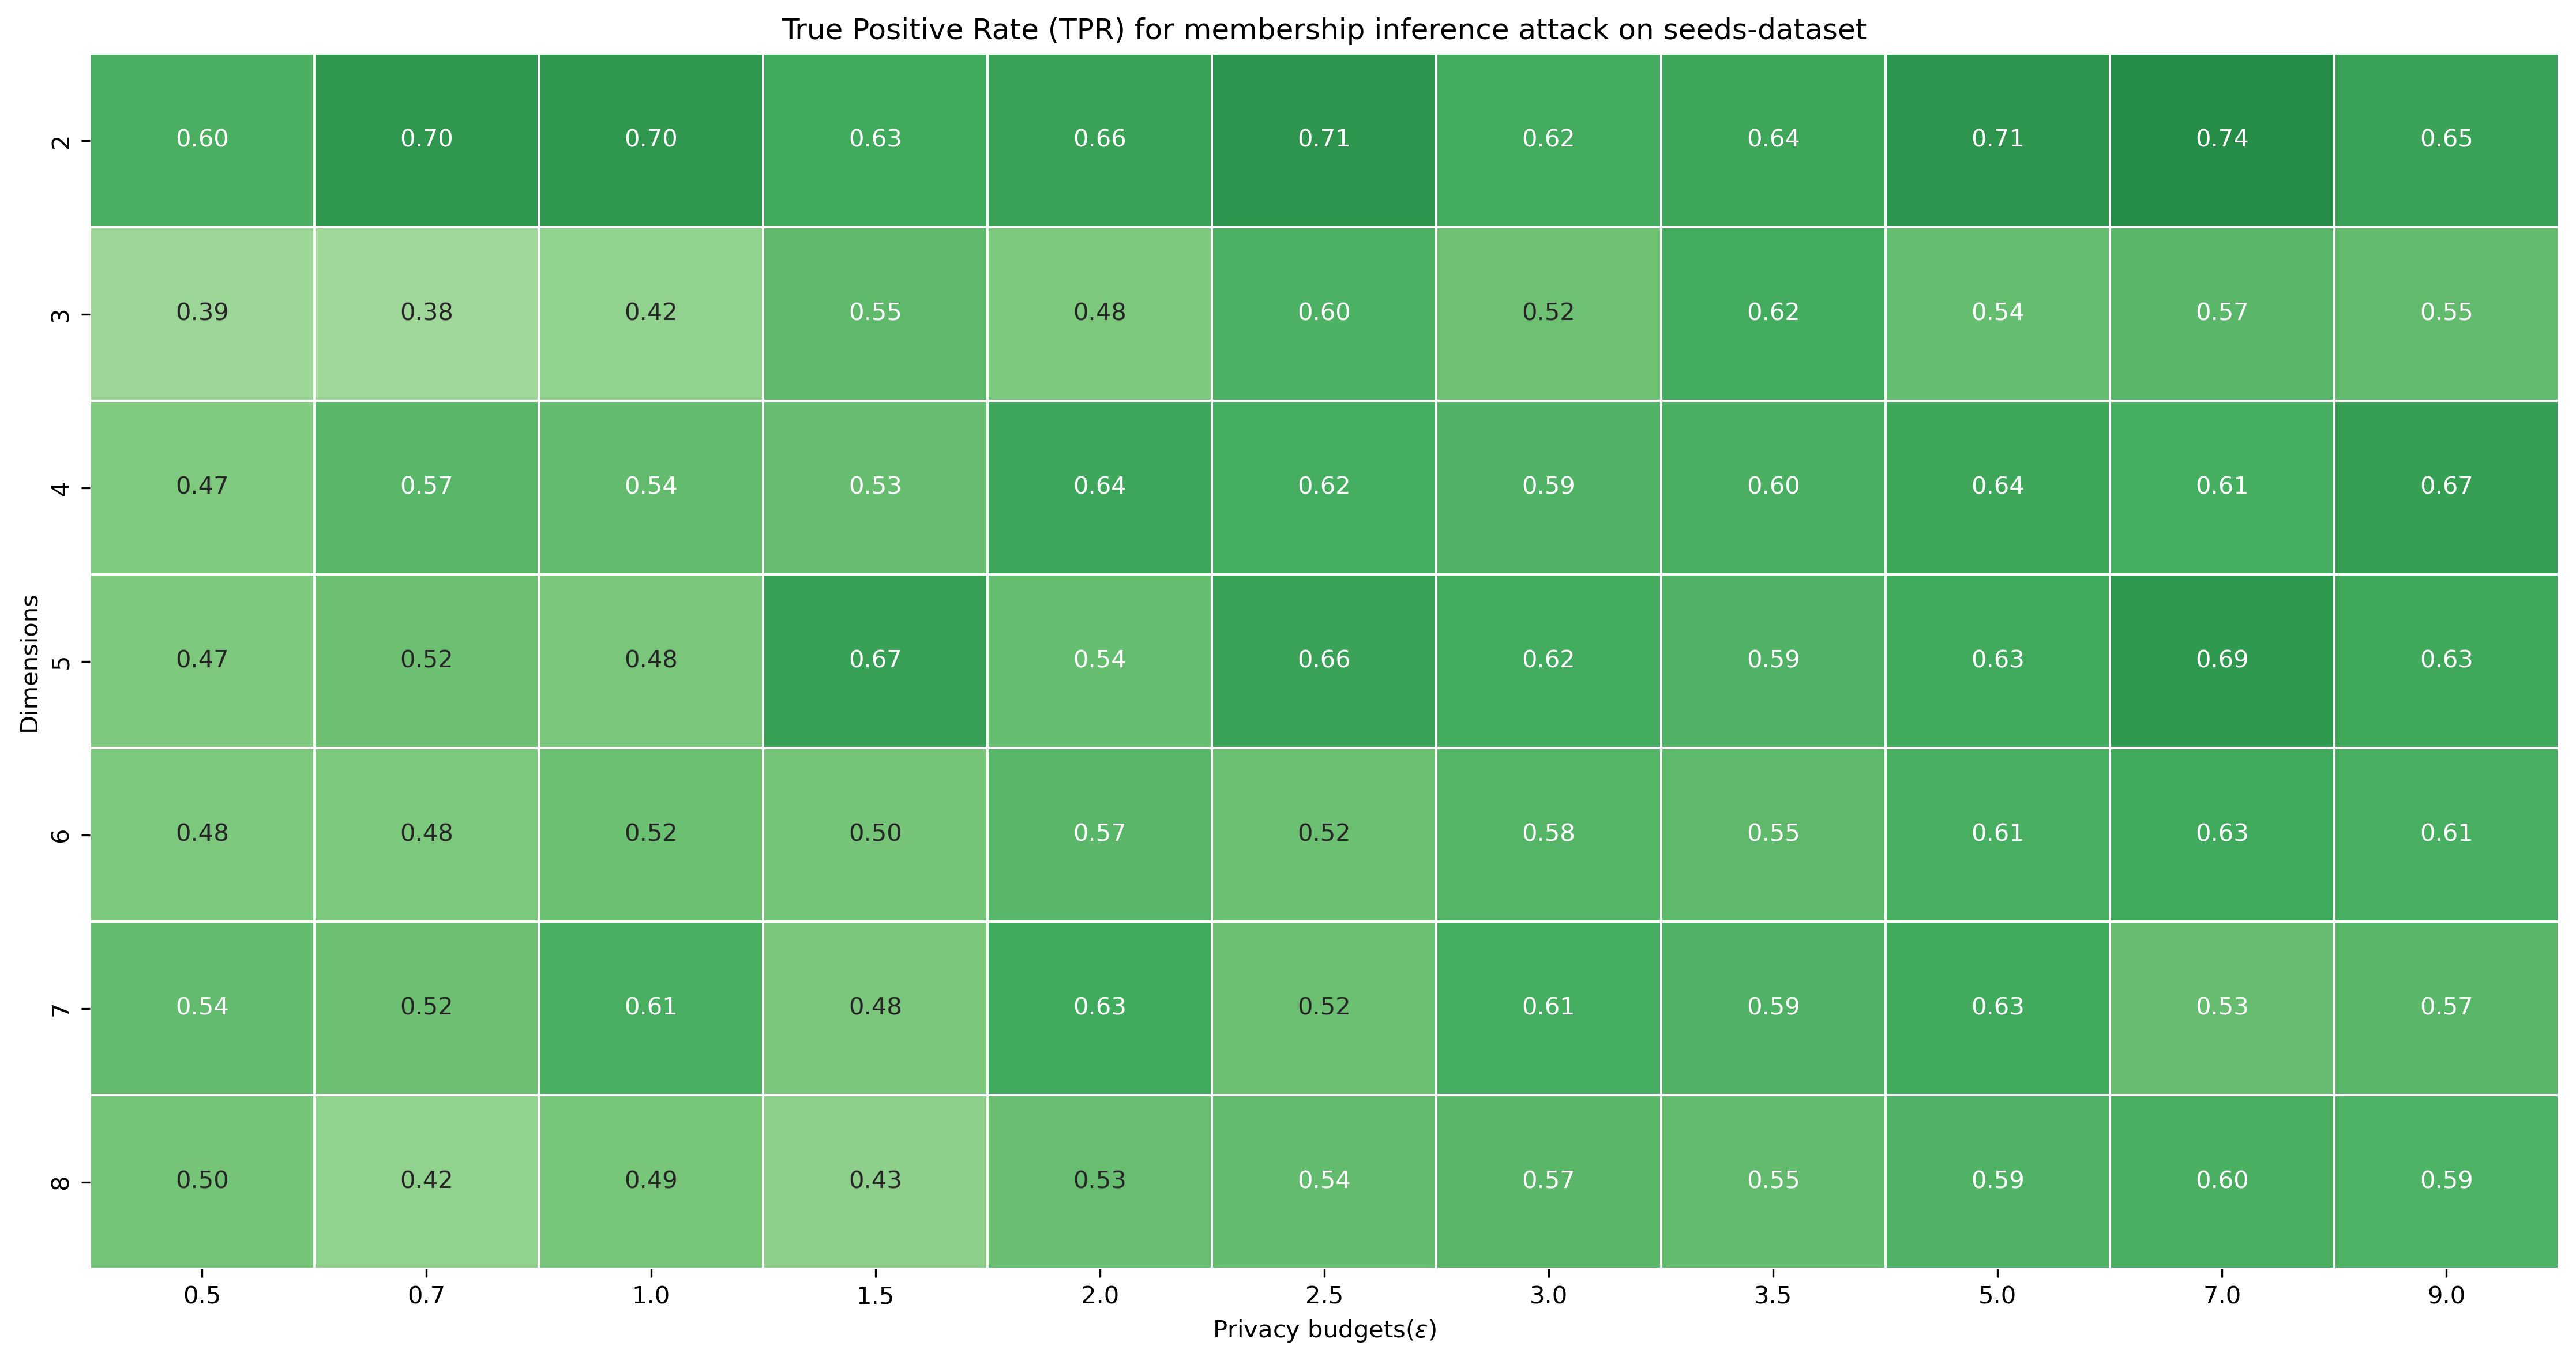
\includegraphics[width=1\textwidth]{Results/kd-laplace/kd-Laplace/seeds-dataset/tpr.png}
            \label{fig:privacy_tpr_seeds-dataset_adversial_advantage_kd-laplace}
        \end{subfigure}
        \vfill % vertical space
        \begin{subfigure}[c]{1\textwidth}
            \caption{\textbf{Heatmap TPR for the Piecewise mechanism, per privacy budget \& dimension for seeds-dataset.}}
            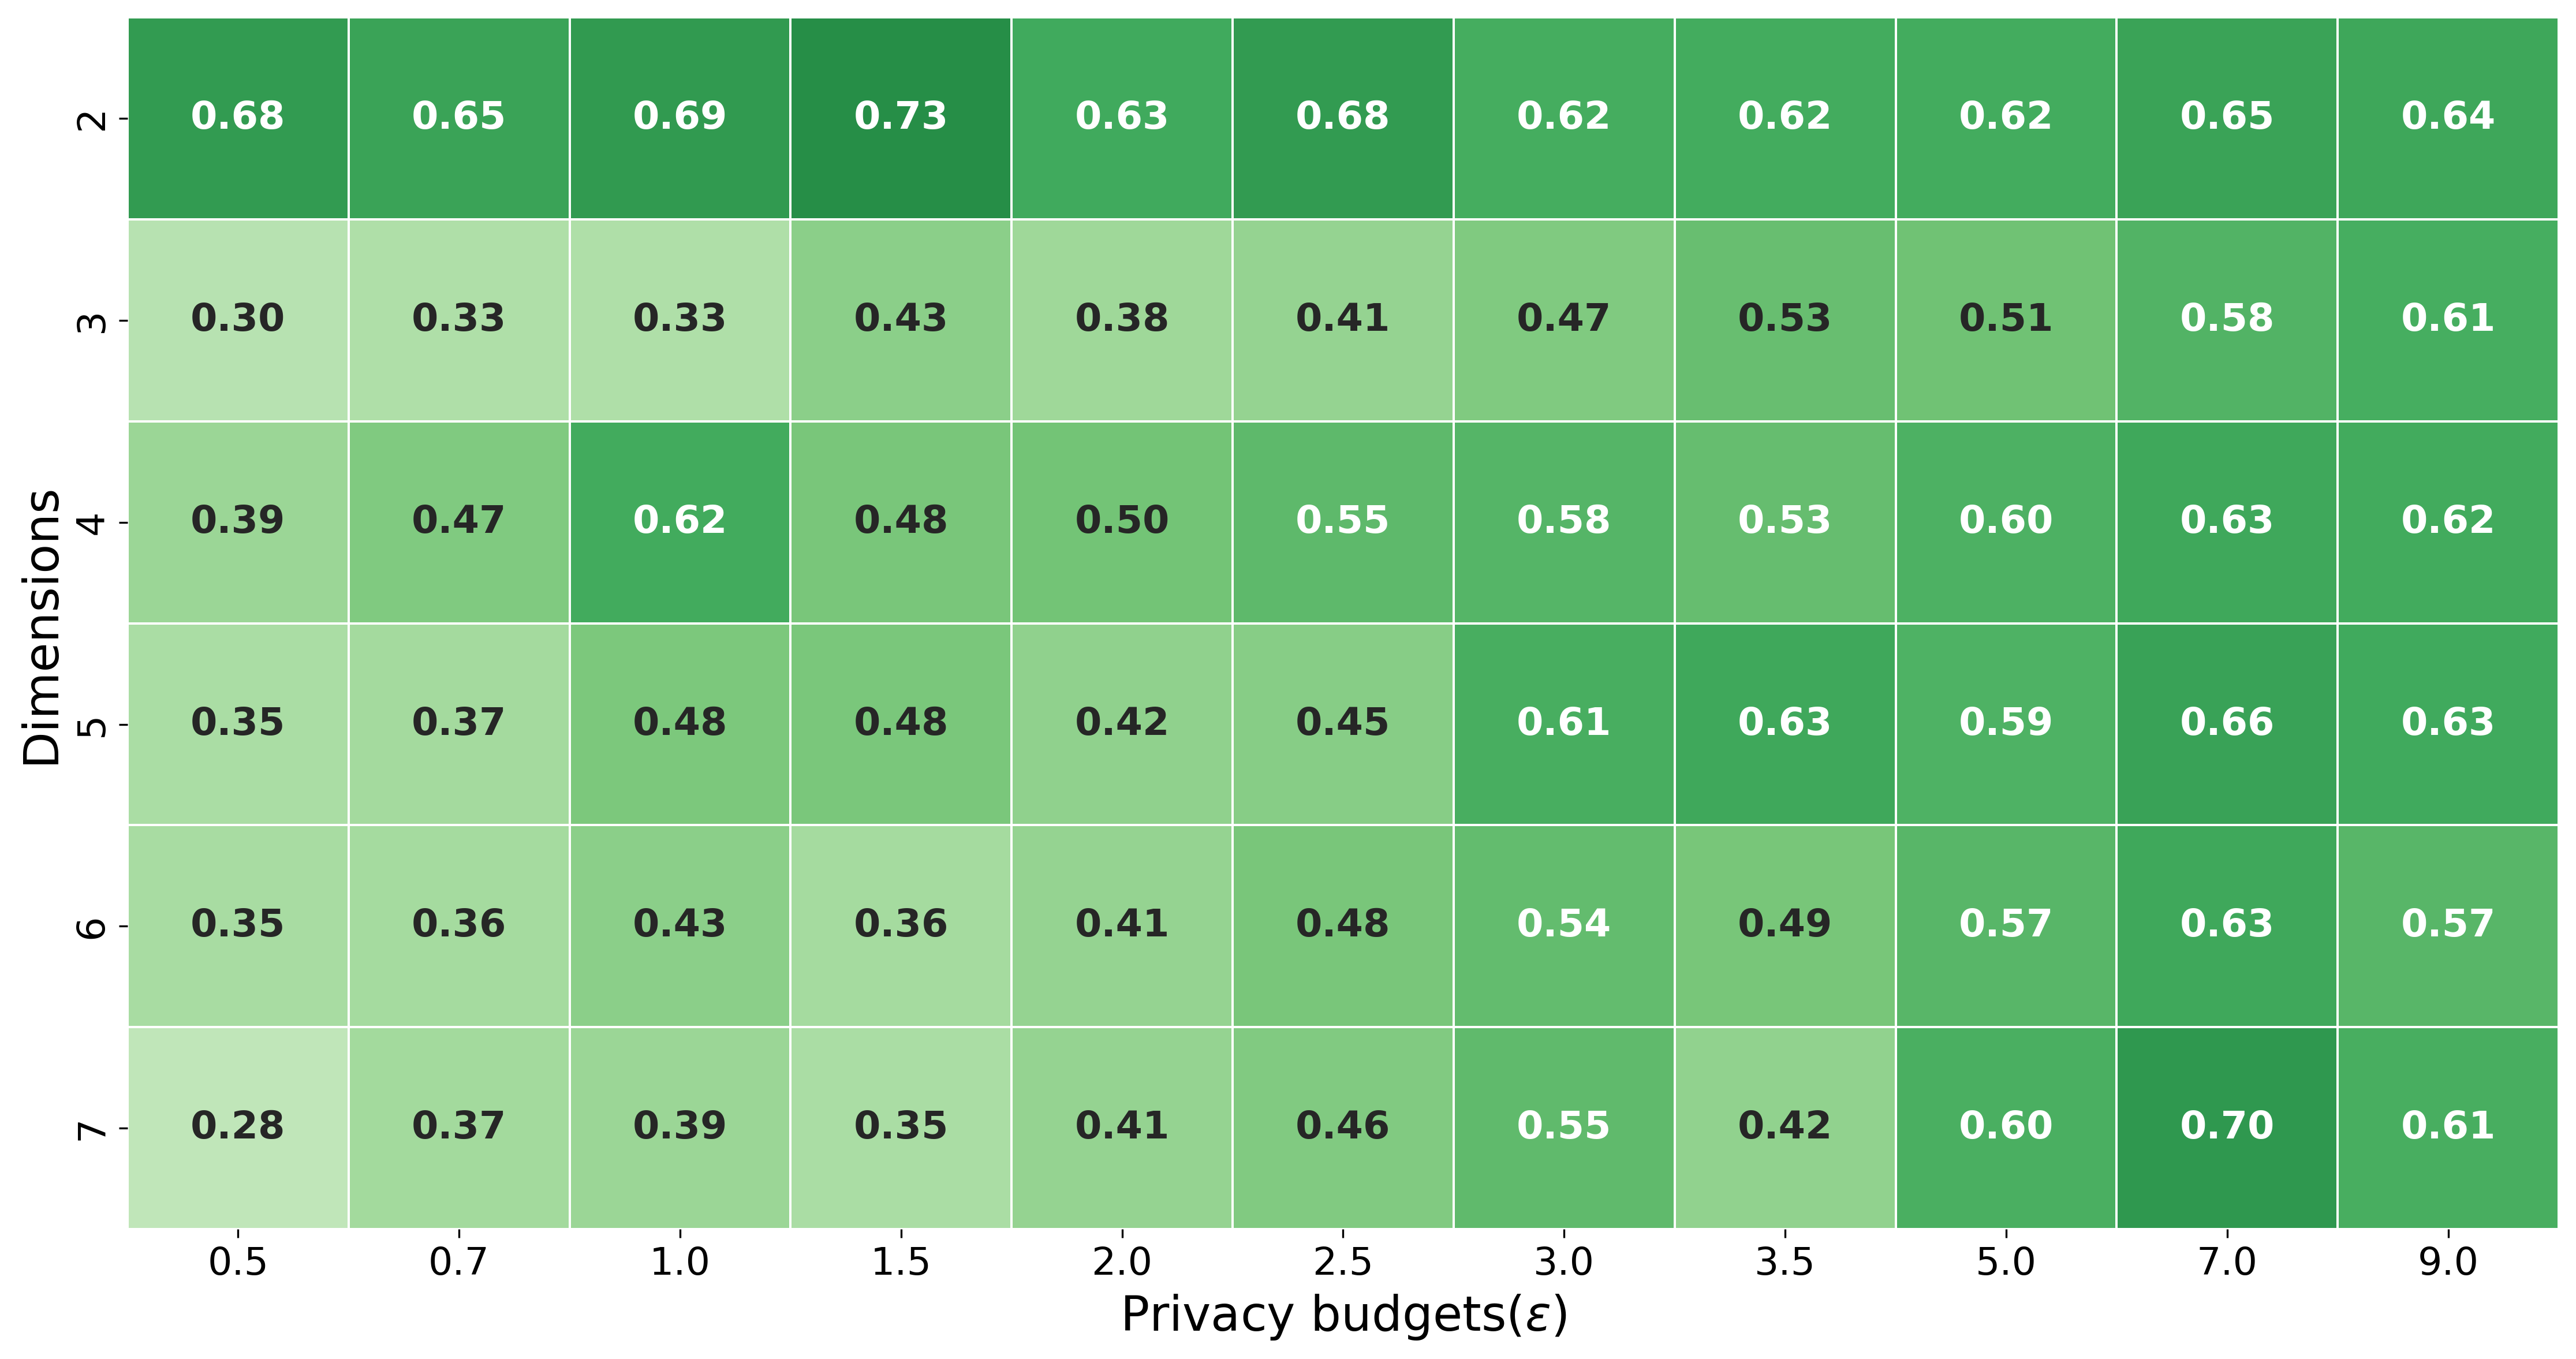
\includegraphics[width=1\textwidth]{Results/kd-laplace/piecewise/seeds-dataset/tpr.png}
            \label{fig:privacy_tpr_seeds-dataset_adversial_advantage_piecewise}
        \end{subfigure}
    \end{subfigure}
\end{figure}
When we examine the plot above, we see a different pattern. For Piecewise, the \gls{tpr} for privacy budgets from 0.5 to 2.5 is around 0.35, while that of nD-Laplace is around 0.45.
For higher privacy budgets, the \gls{tpr} for both increases to 0.65.
From the \gls{tpr}, it can be inferred that a higher privacy budget indeed leaks more information.
The dimensions have little impact on this, but for both mechanisms, it's observable that 2-dimensions have the highest \gls{tpr}, thereby leaking the most information.
\todo[inline]{Why higher for 2D?}

\newpage
\subsection{Heart dataset}
\begin{figure}[H]
  \centering
  \begin{subfigure}[b]{0.75\textwidth}
    \begin{subfigure}[c]{1\textwidth}
      \caption{\textbf{Heatmap showing adversary advantage for the nD-Laplace mechanism, per privacy budget \& dimension for heart-dataset.}}
      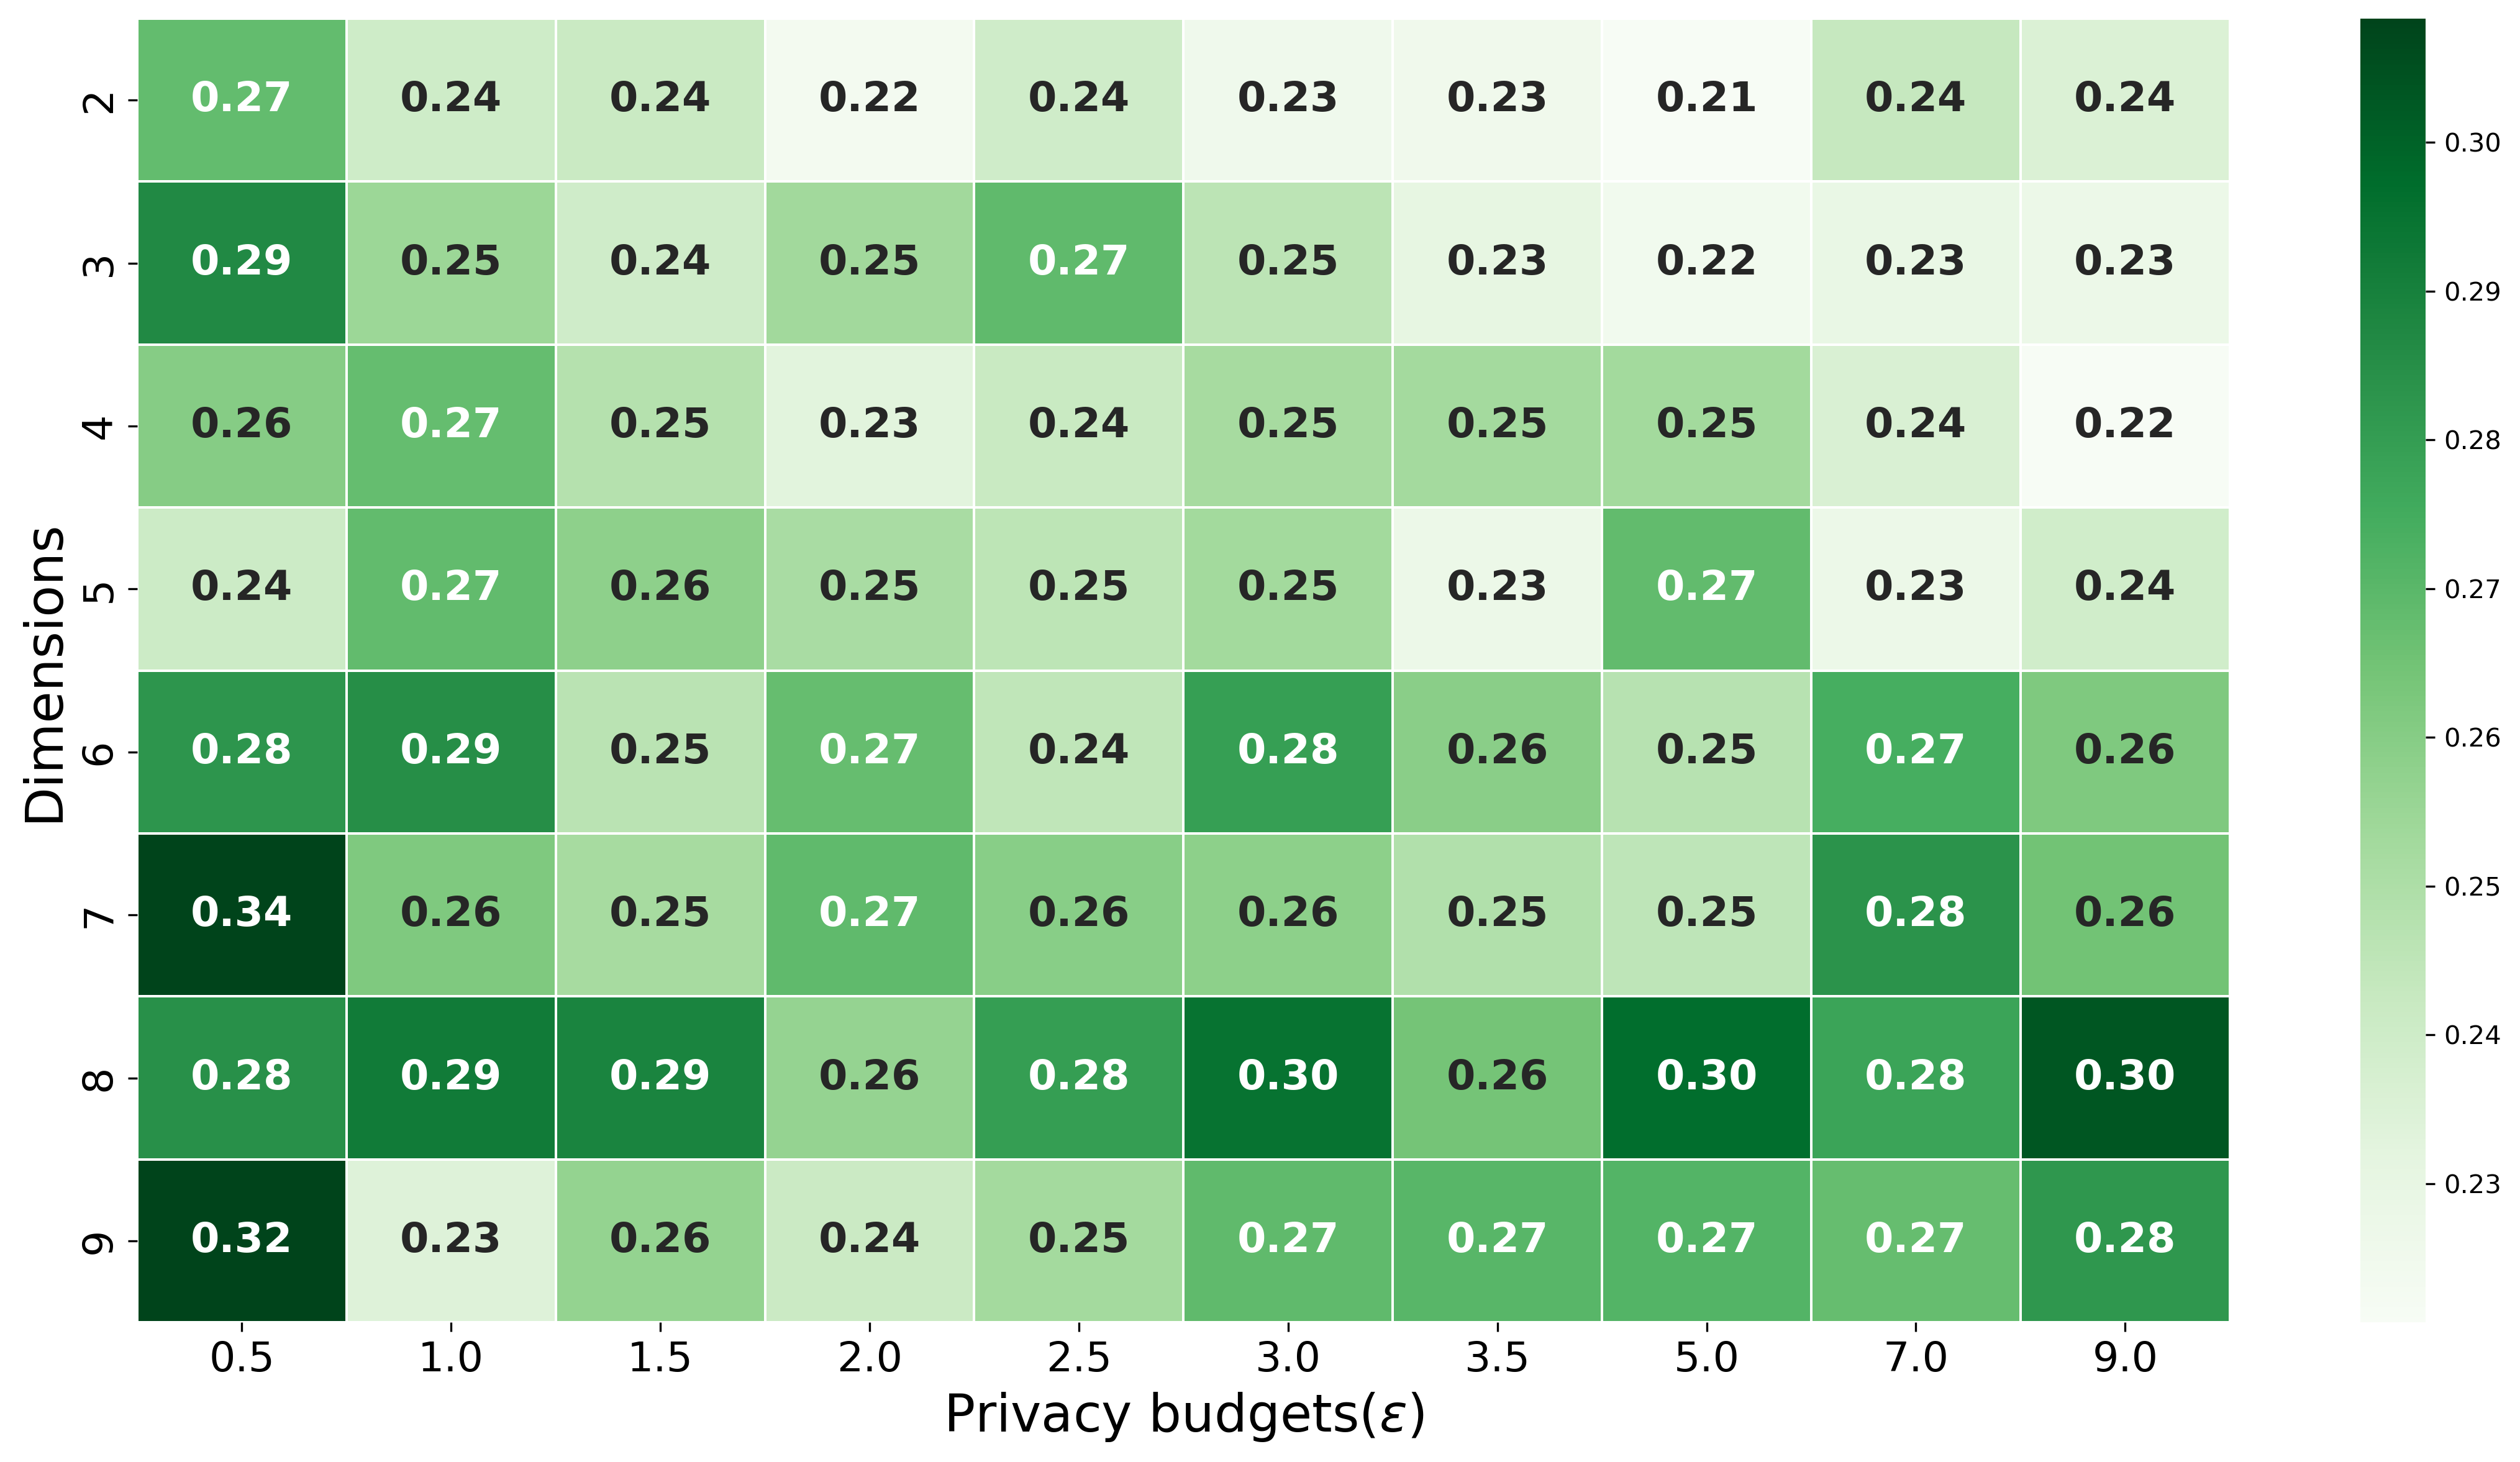
\includegraphics[width=1\textwidth]{Results/nd-laplace/nd-Laplace/heart-dataset/shokri_mi_adv.png}
      \label{fig:privacy_heart-dataset_adversial_advantage_kd-laplace}
    \end{subfigure}
    \vfill % vertical space

    \begin{subfigure}[c]{1\textwidth}
      \caption{\textbf{Heatmap showing adversary advantage for the Piecewise mechanism, per privacy budget \& dimension for heart-dataset.}}
      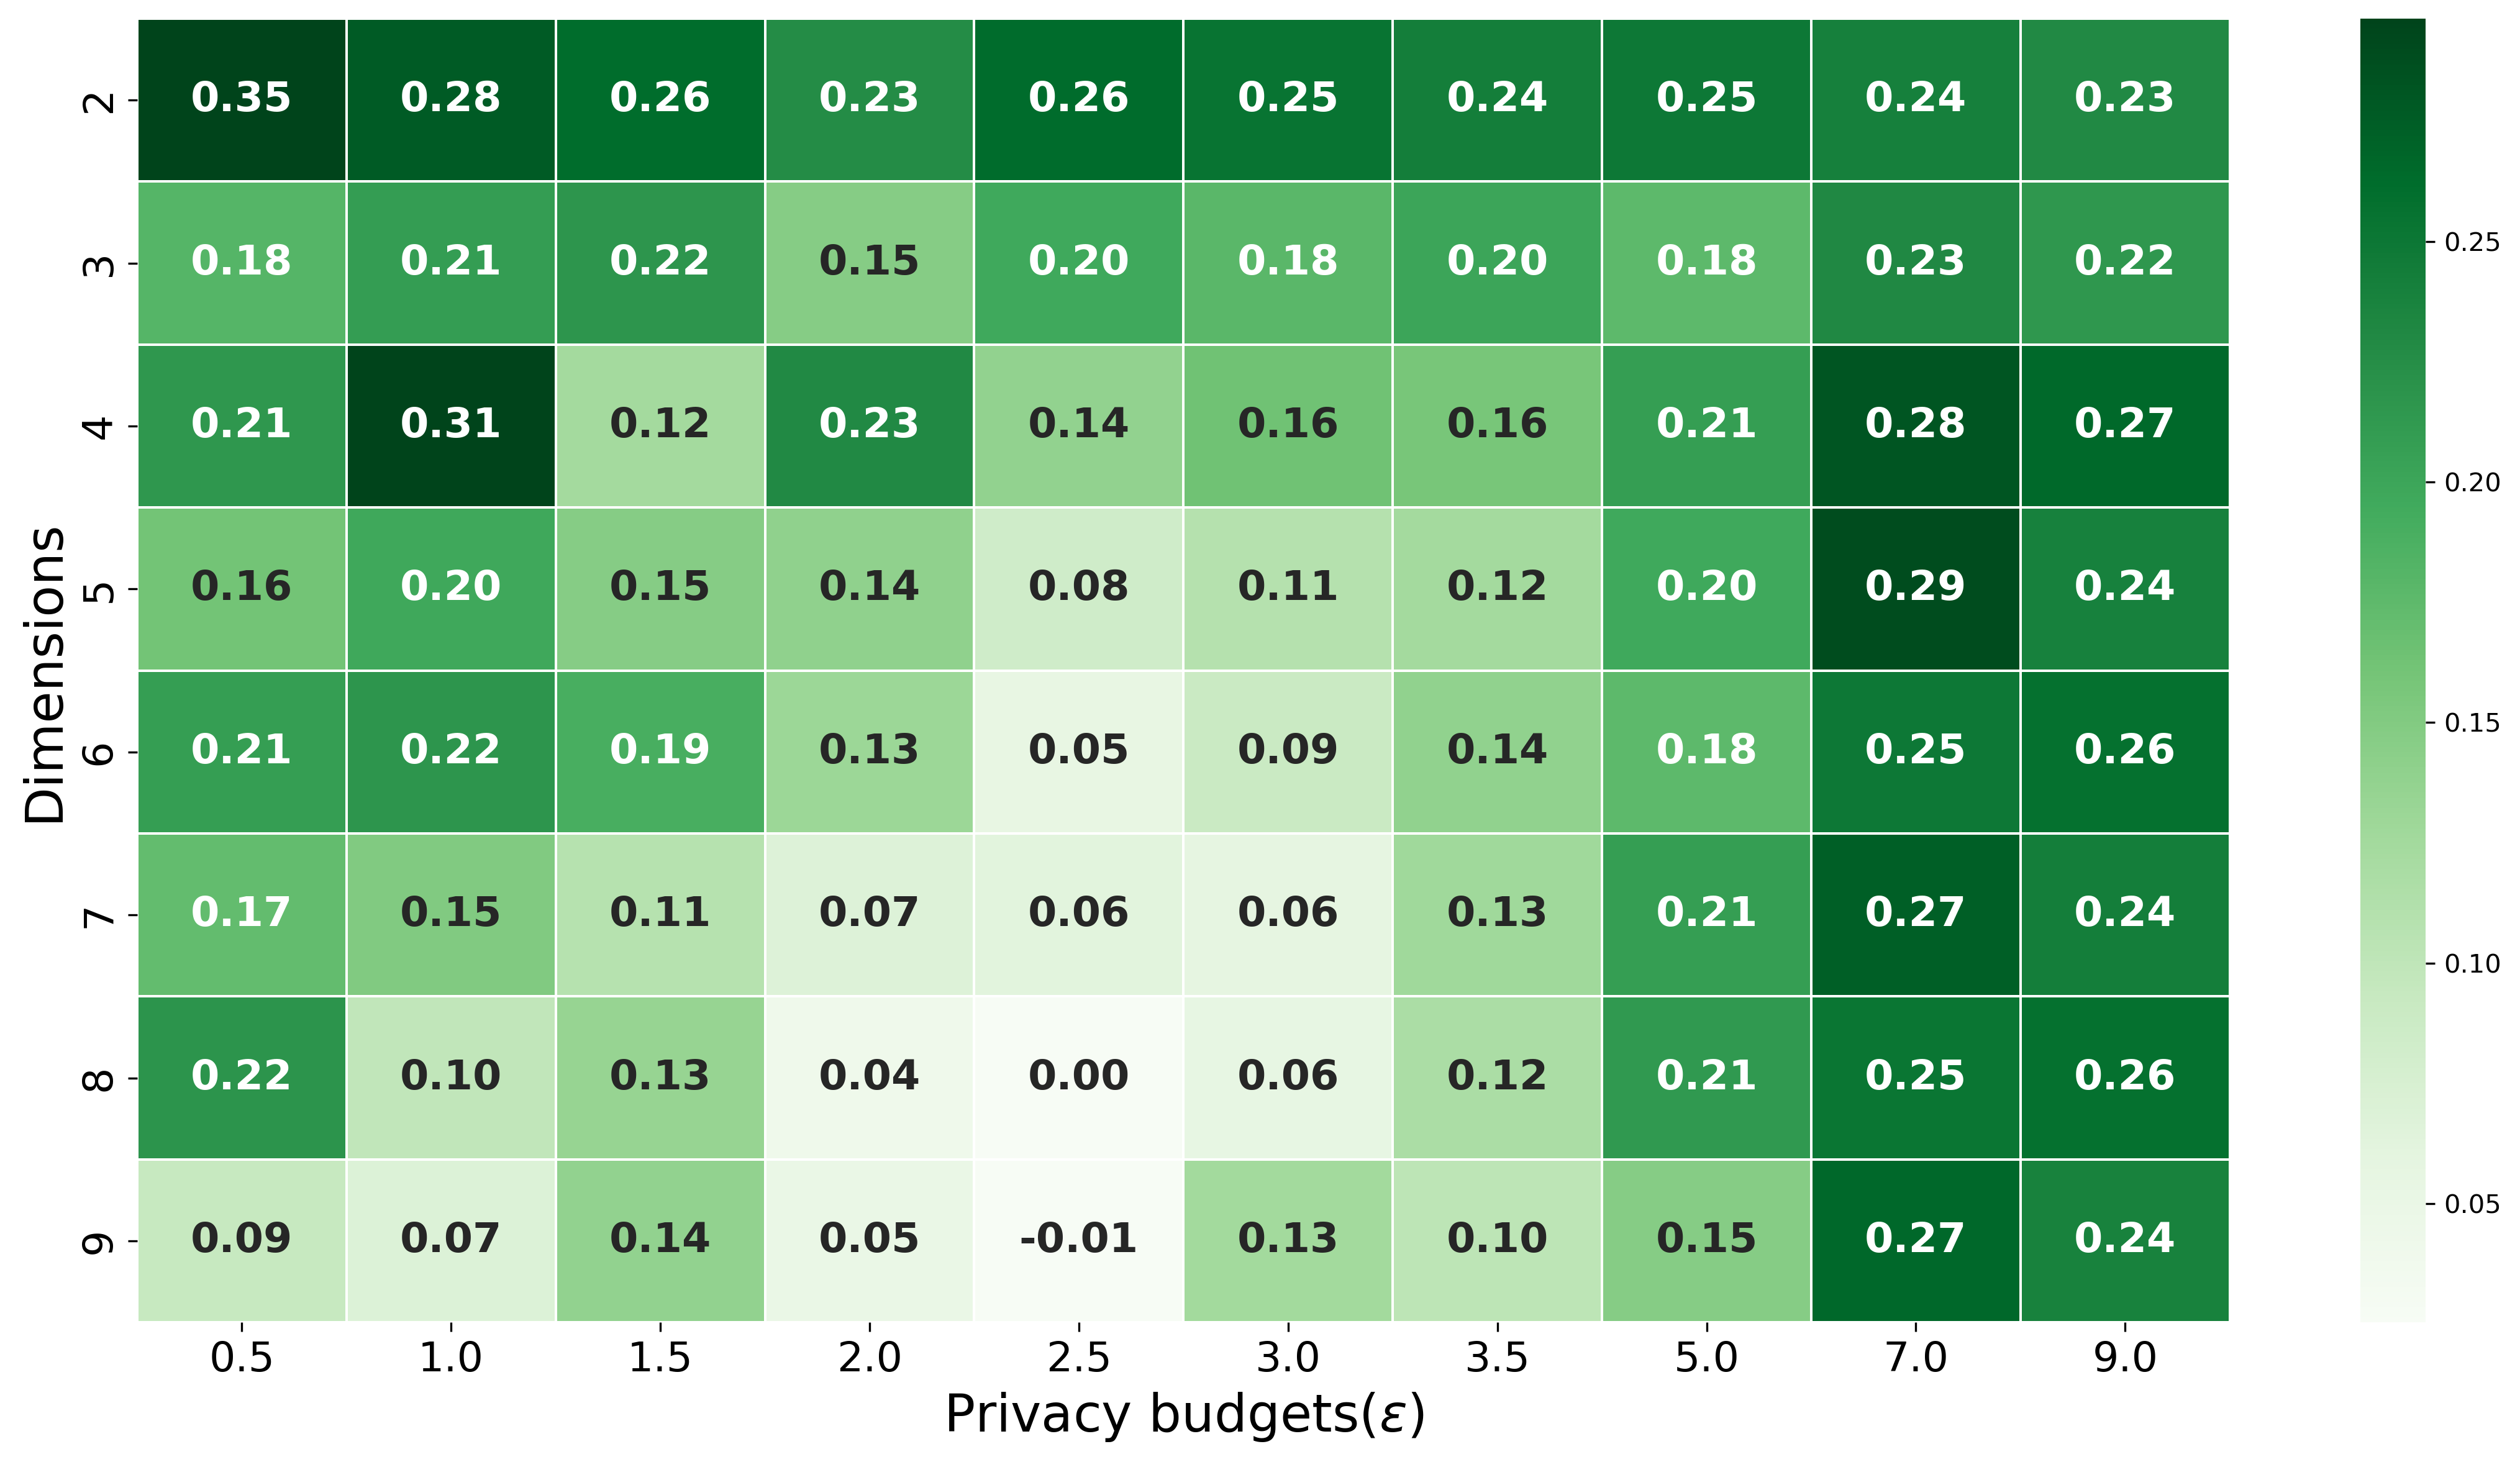
\includegraphics[width=1\textwidth]{Results/nd-laplace/piecewise/heart-dataset/shokri_mi_adv.png}
      \label{fig:privacy_heart-dataset_adversial_advantage_piecewise}
    \end{subfigure}
  \end{subfigure}
\end{figure}
For the nD-Laplace mechanism, there's little difference observed between the privacy budgets and dimensions. This is expected, as there's also minimal variation in the \gls{ami} score across different privacy budgets. However, a correlation can be seen between lower dimensions (2 / 3) and the impact of higher privacy budgets. For these dimensions, the adversary advantage is approximately 5 points lower than the other dimensions.
With the Piecewise mechanism, a similar result is observed, but it's evident that higher dimensions (8 and 9) have an impact on privacy budgets ranging from 0.5 to 3. For 2-dimensions, the score also seems significantly higher than the rest.
Although the adversary advantage in these heatmaps follows a somewhat more logical progression (increasing from left to right), we will also analyze the \gls{tpr} on the following page. 
\newpage
\begin{figure}[H]
    \centering
    \begin{subfigure}[b]{0.75\textwidth}
        \begin{subfigure}[c]{1\textwidth}
            \caption{\textbf{Heatmap TPR for the kD-Laplace mechanism, per privacy budget \& dimension for heart-dataset.}}
            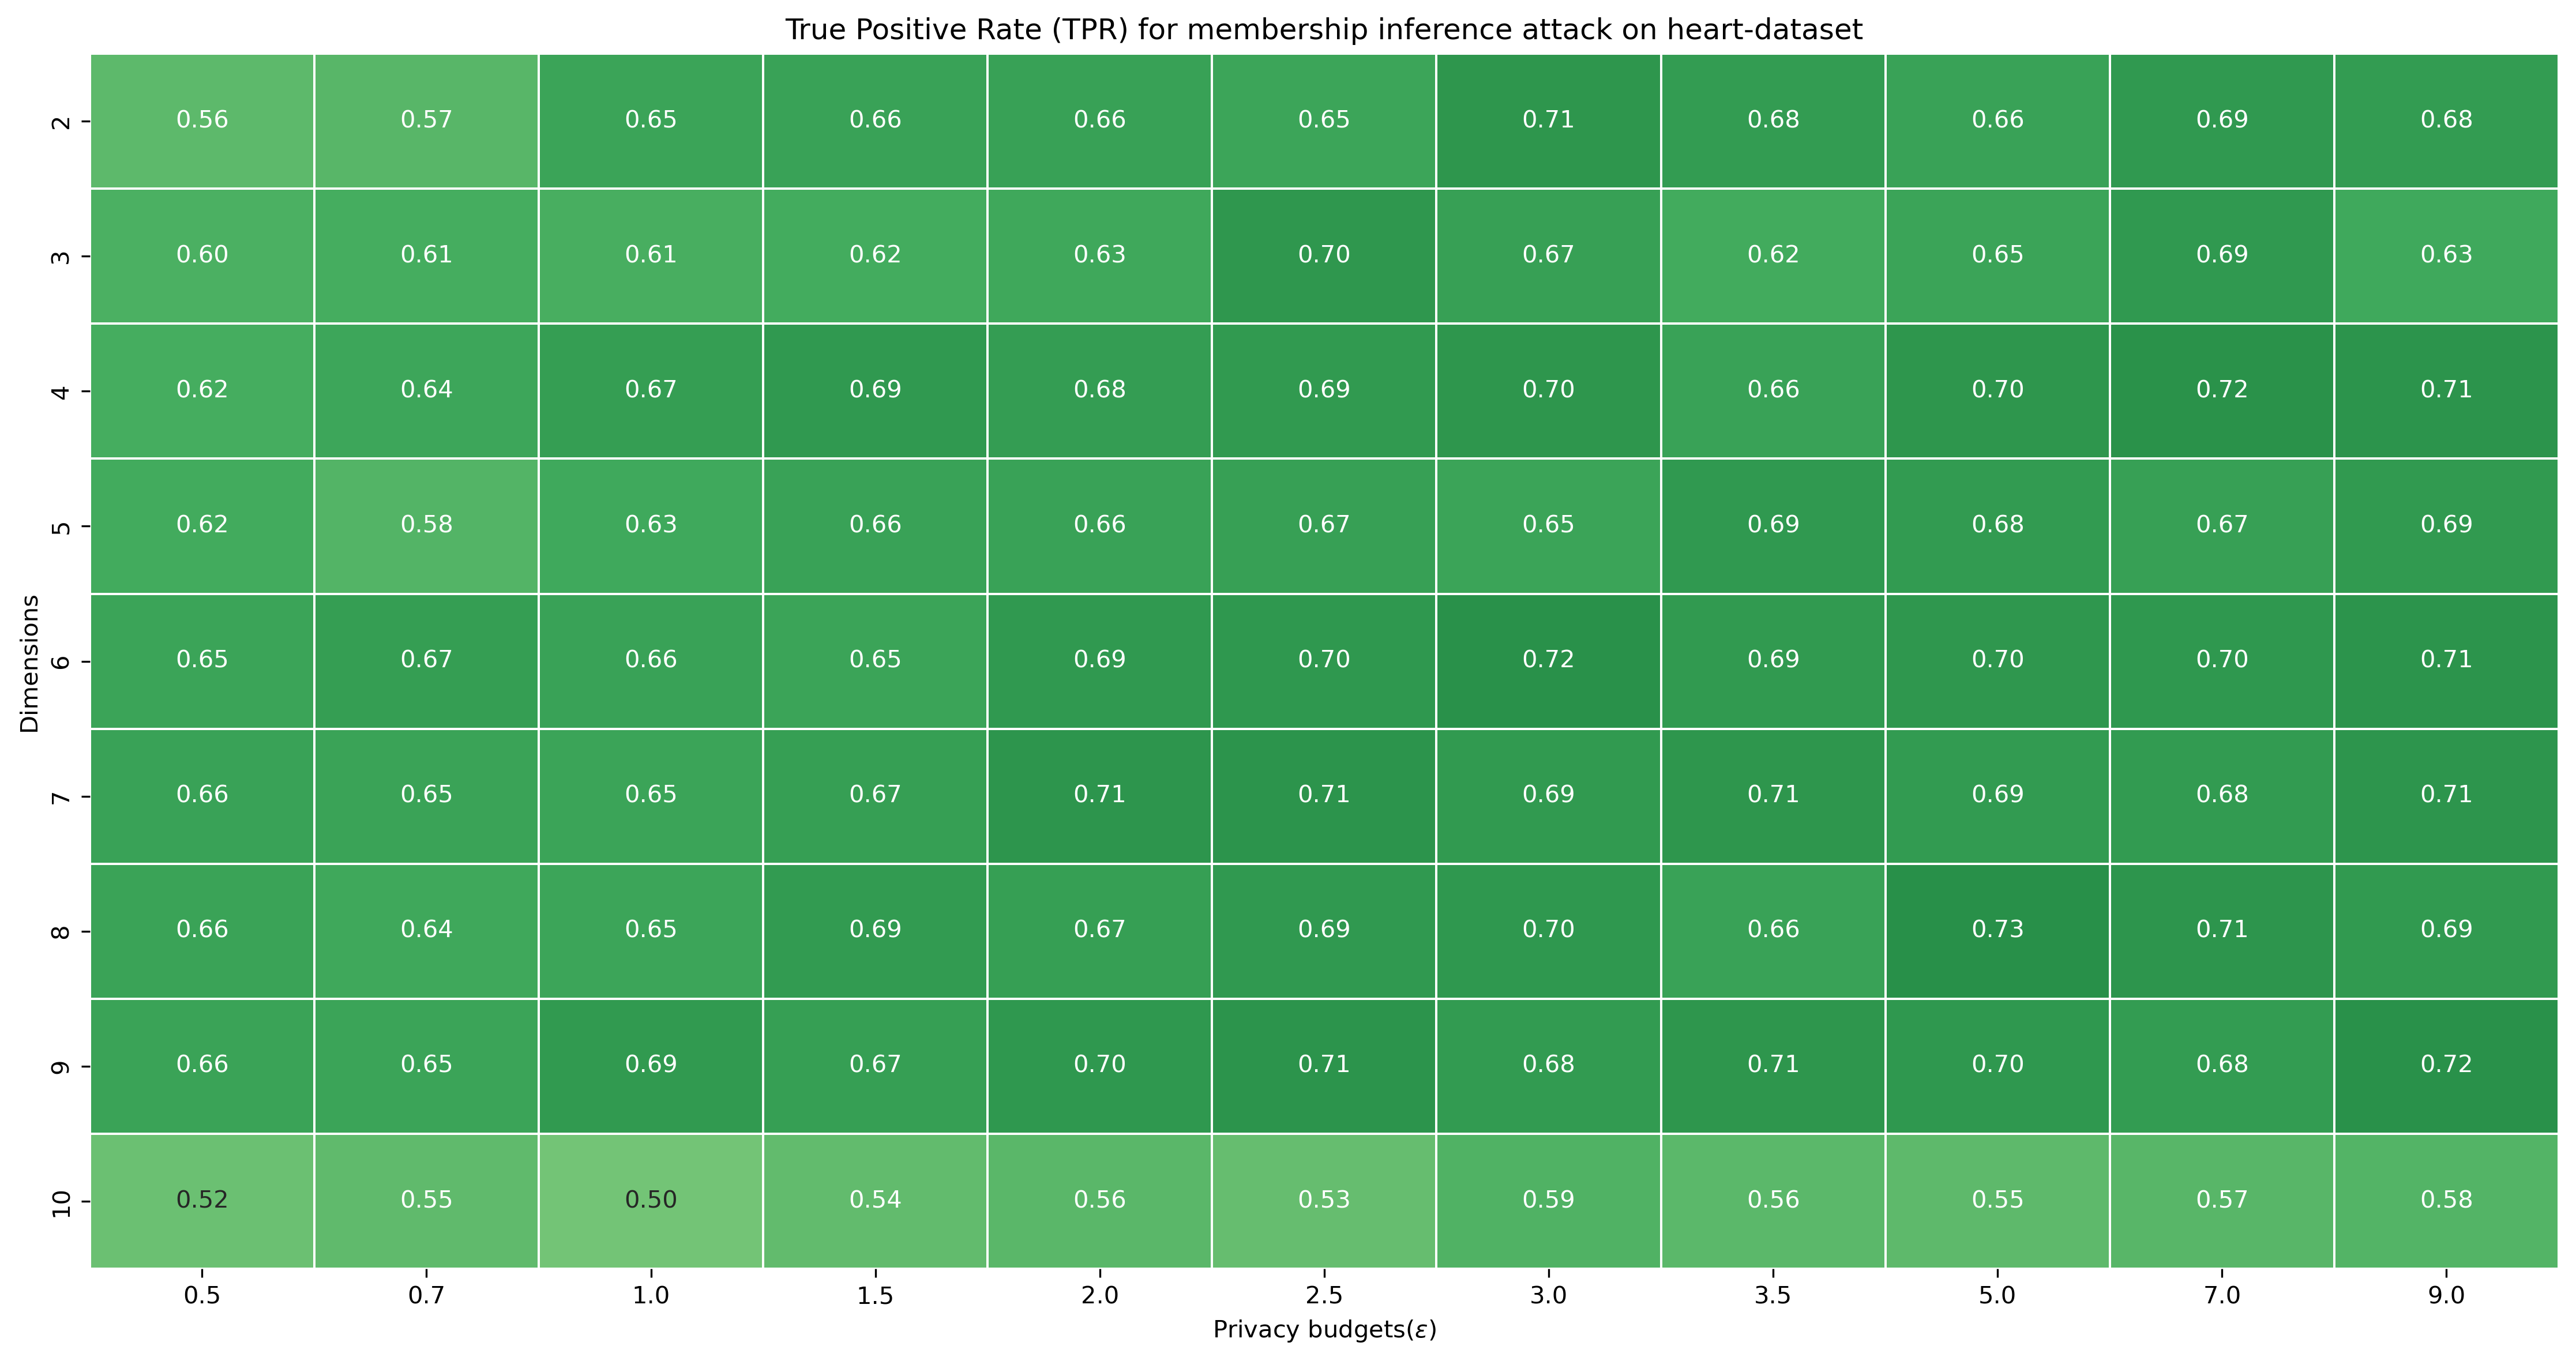
\includegraphics[width=1\textwidth]{Results/kd-laplace/kd-Laplace/heart-dataset/tpr.png}
            \label{fig:privacy_tpr_heart-dataset_adversial_advantage_kd-laplace}
        \end{subfigure}
        \vfill % vertical space

        \begin{subfigure}[c]{1\textwidth}
            \caption{\textbf{Heatmap TPR for the Piecewise mechanism, per privacy budget \& dimension for heart-dataset.}}
            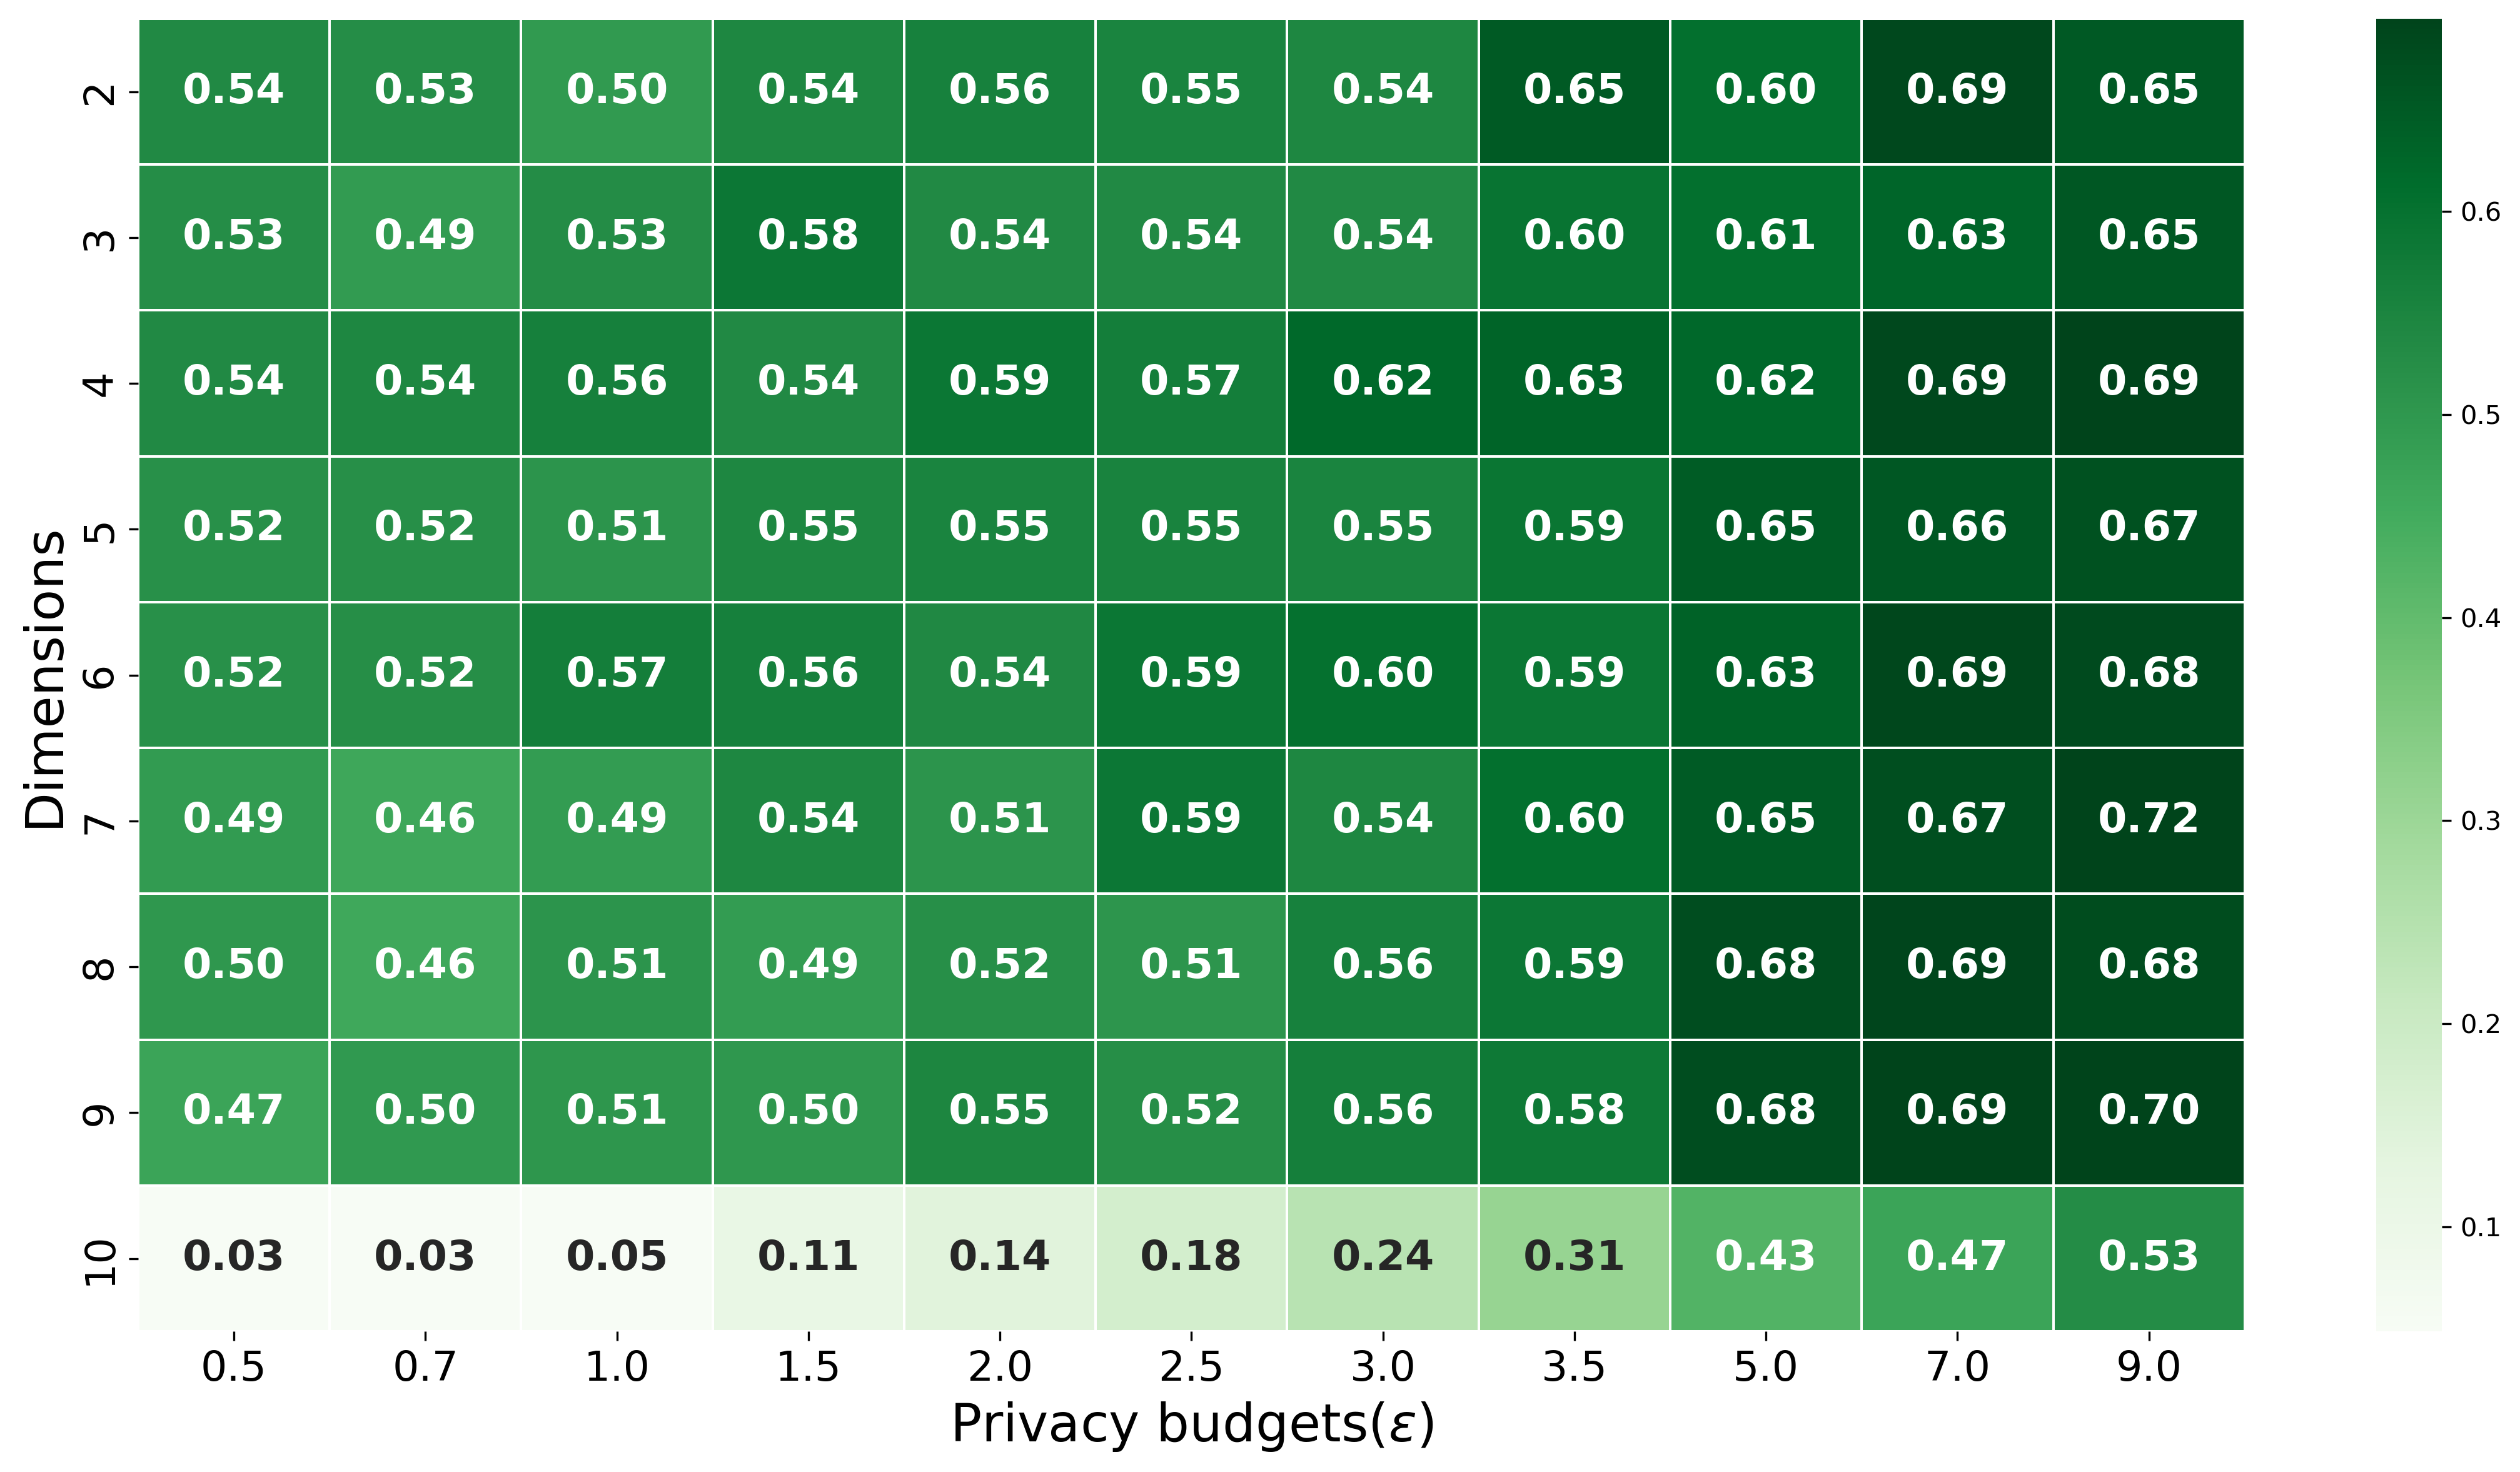
\includegraphics[width=1\textwidth]{Results/kd-laplace/piecewise/heart-dataset/tpr.png}
            \label{fig:privacy_tpr_heart-dataset_adversial_advantage_piecewise}
        \end{subfigure}
    \end{subfigure}
\end{figure}
The Piecewise mechanism's \gls{tpr} results are very explicit and clear. 
There is a 
\newpage

\subsection{Circle dataset}
\begin{figure}[H]
  \centering
  \begin{subfigure}[b]{0.85\textwidth}
    \begin{subfigure}[c]{1\textwidth}
      \caption{\textbf{Heatmap showing adversary advantage for the kD-Laplace mechanism, per privacy budget \& dimension for circle-dataset.}}
      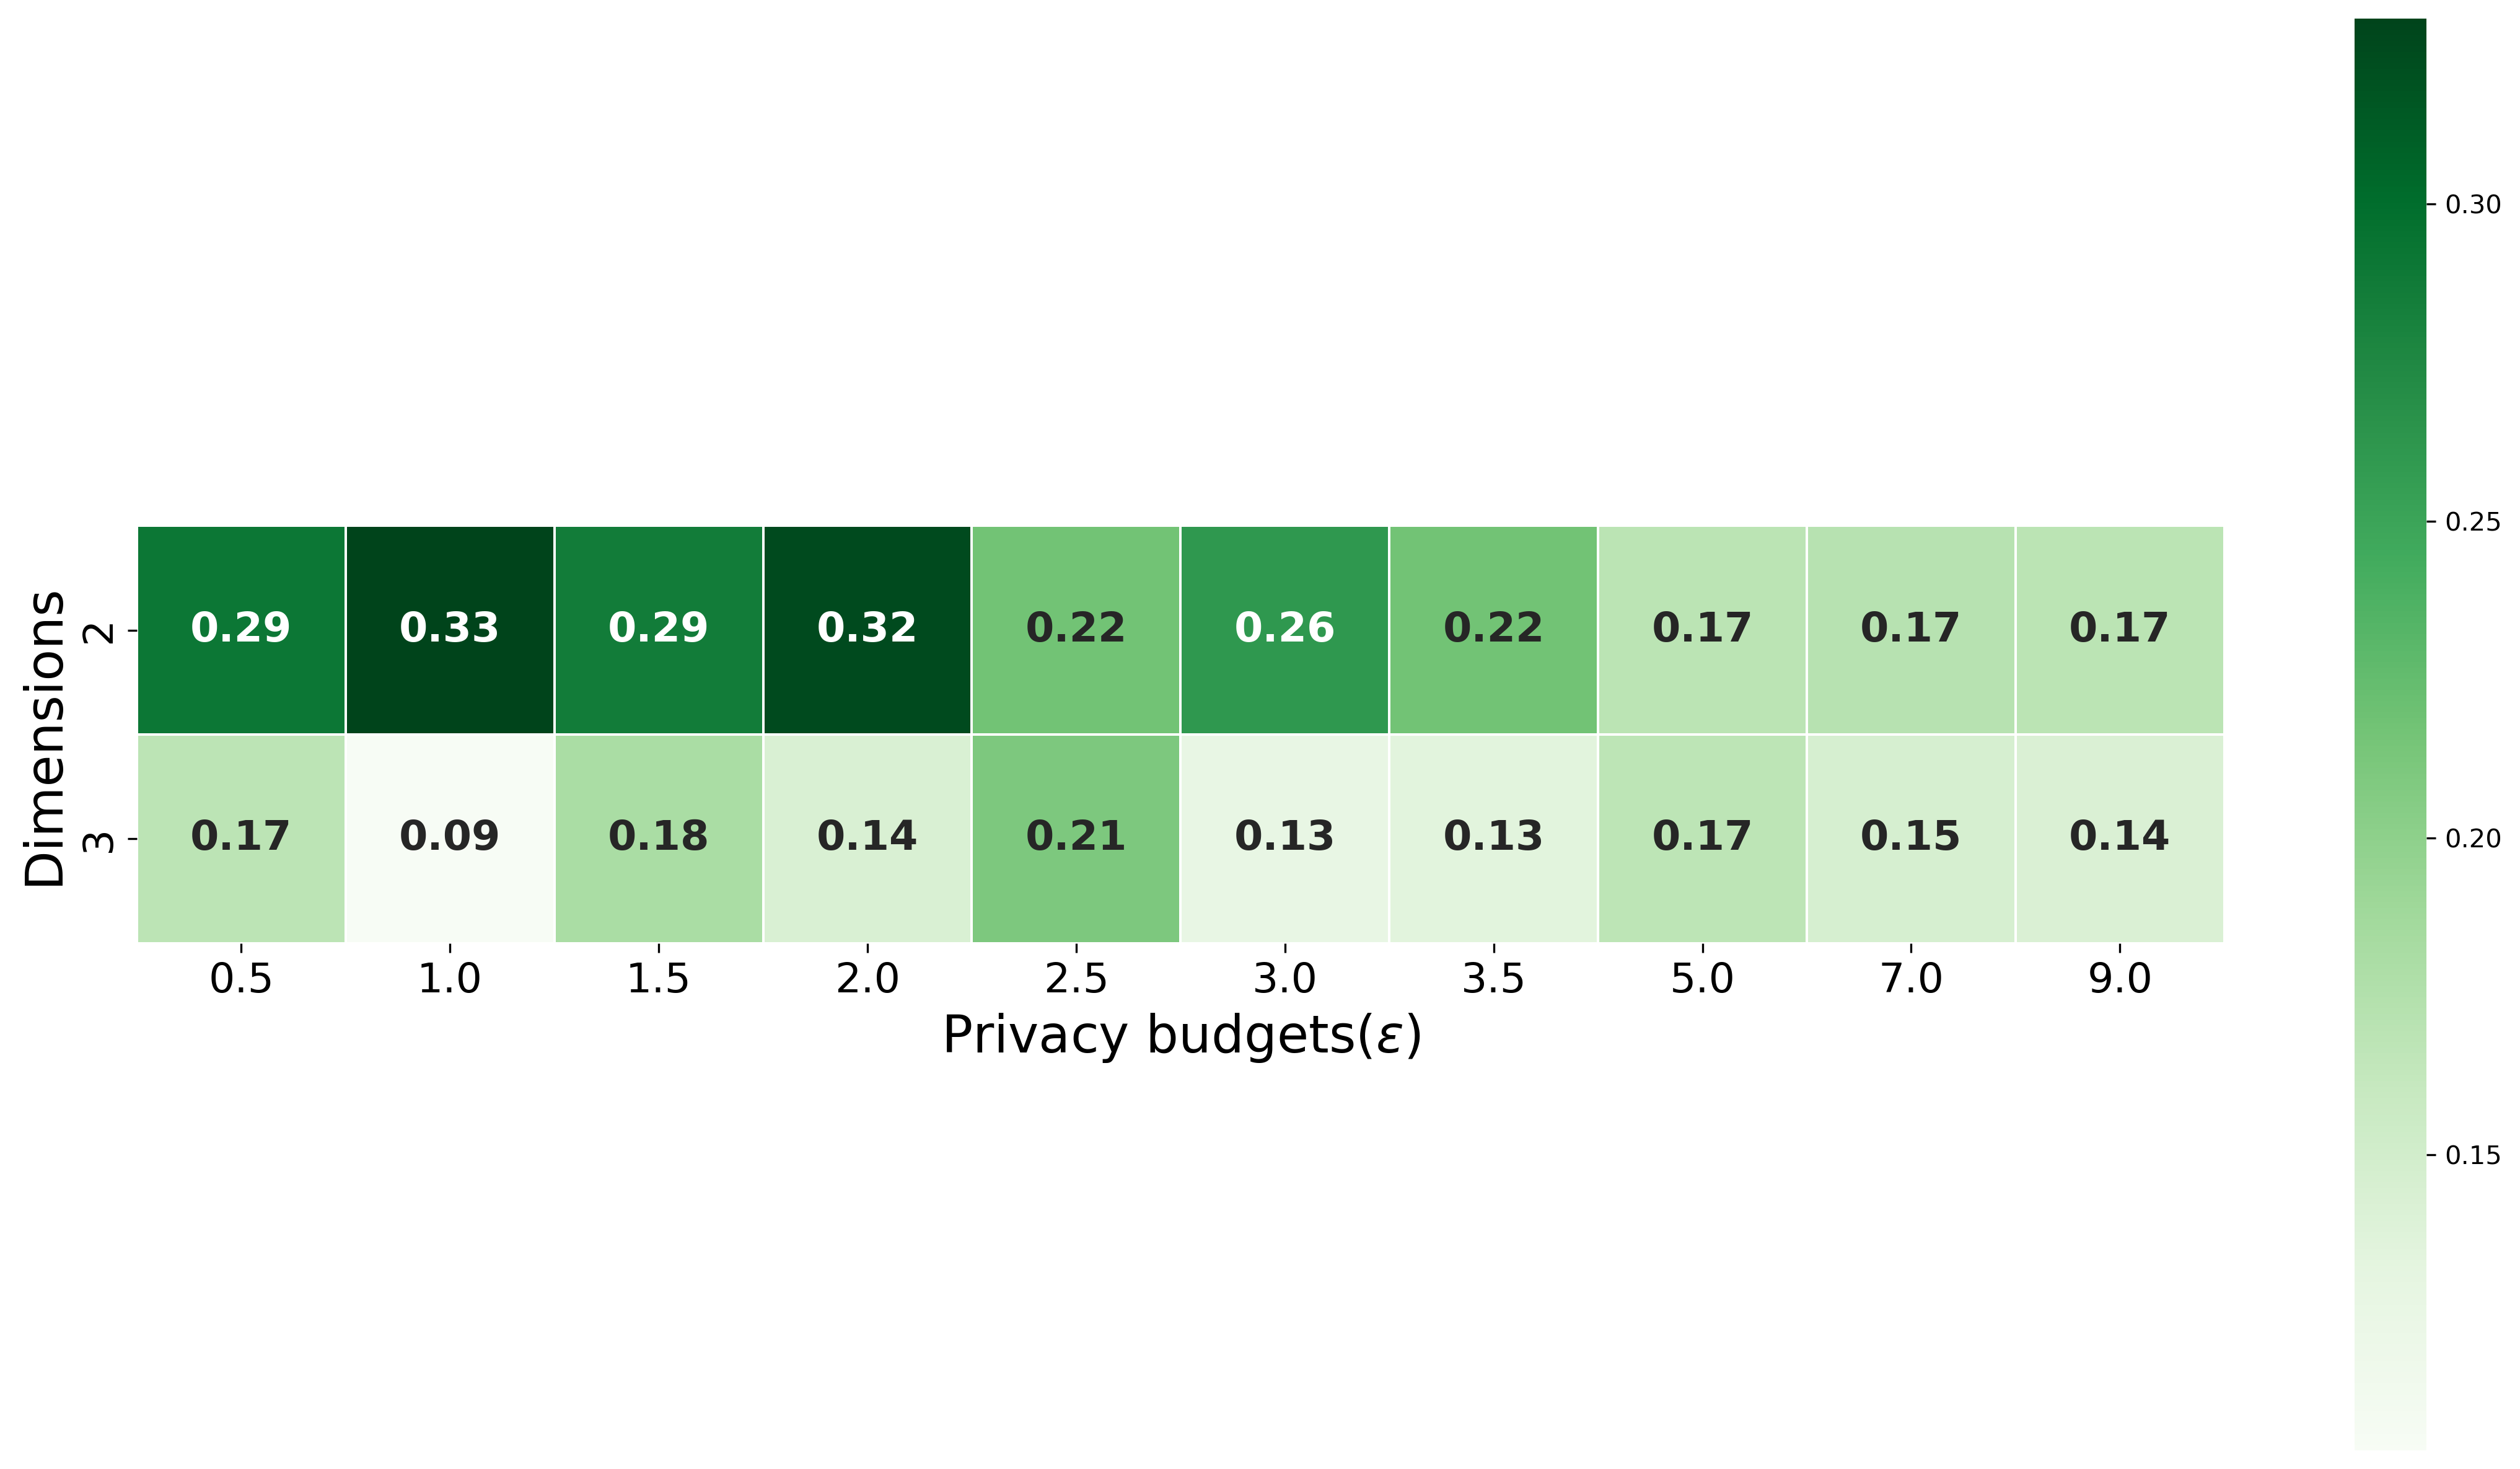
\includegraphics[width=1\textwidth]{Results/nd-laplace/nd-Laplace/circle-dataset/shokri_mi_adv.png}
      \label{fig:privacy_circle-dataset_adversial_advantage_kd-laplace}
    \end{subfigure}
    \vfill % vertical space

    \begin{subfigure}[c]{1\textwidth}
      \caption{\textbf{Heatmap showing adversary advantage for the Piecewise mechanism, per privacy budget \& dimension for seeds-dataset.}}
      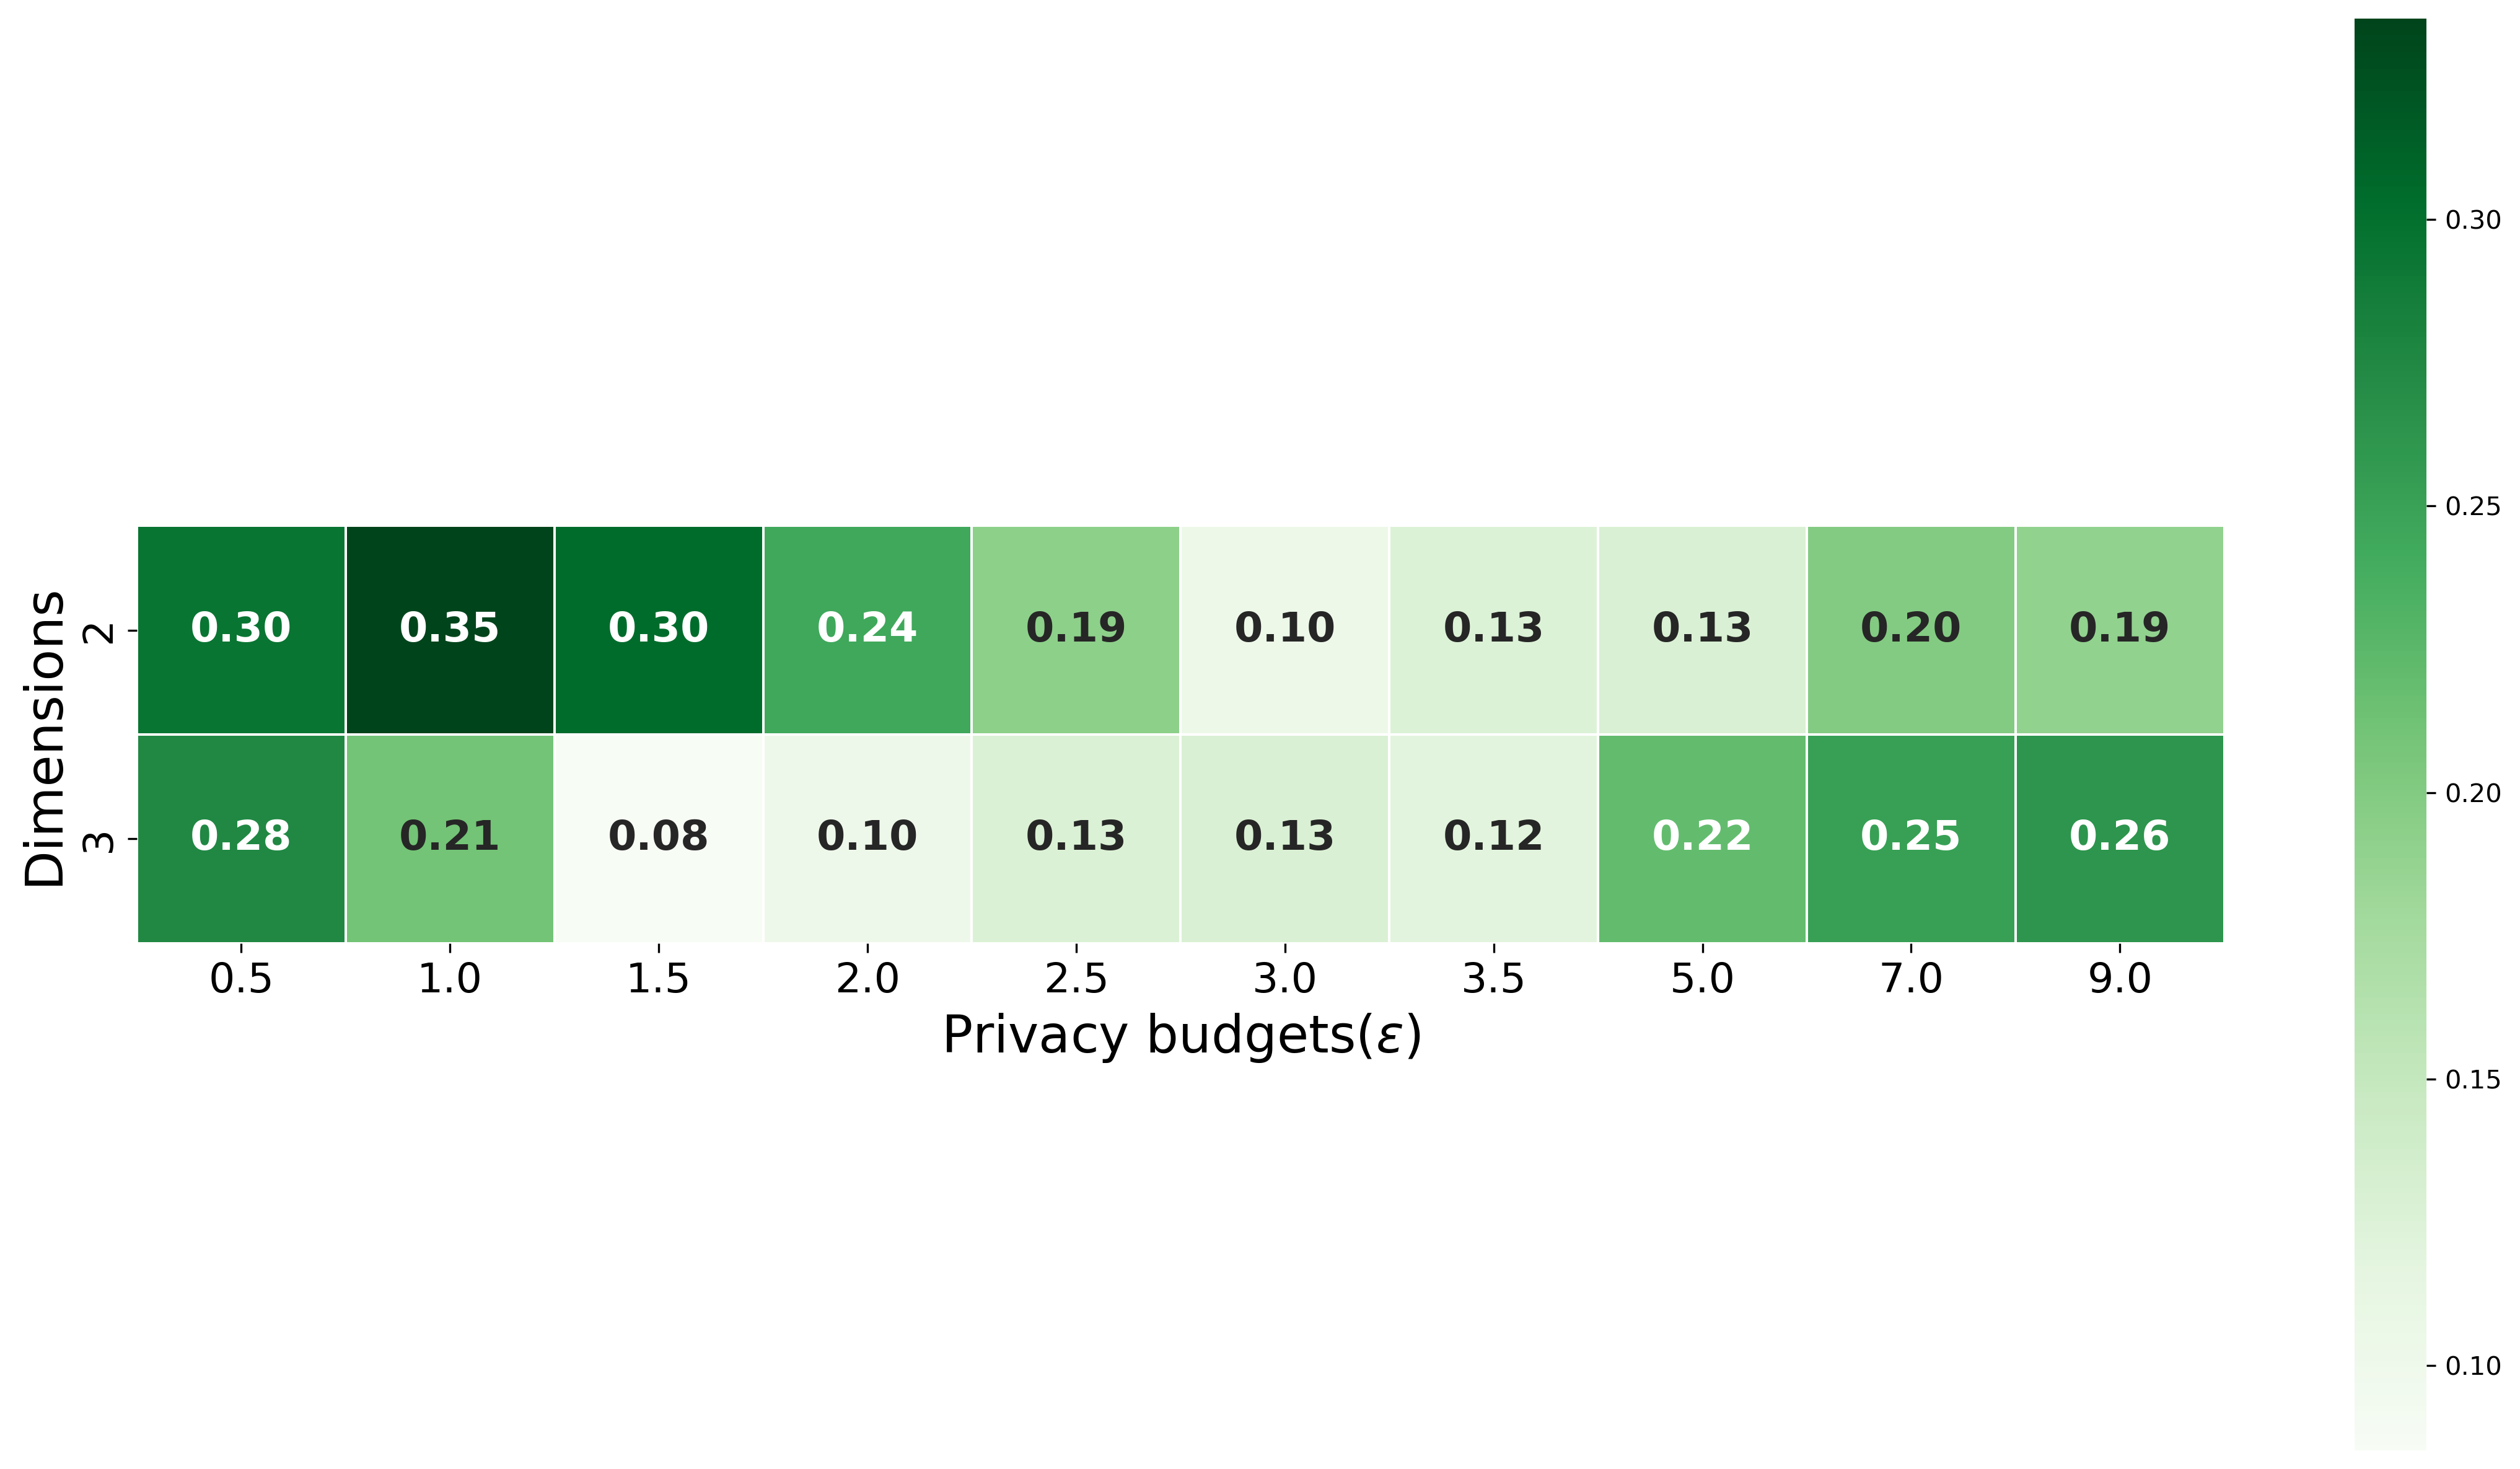
\includegraphics[width=1\textwidth]{Results/nd-laplace/piecewise/circle-dataset/shokri_mi_adv.png}
      \label{fig:privacy_circle-dataset_adversial_advantage_piecewise}
    \end{subfigure}
  \end{subfigure}
\end{figure}

\newpage
\subsection{Line dataset}
\begin{figure}[H]
  \centering
  \begin{subfigure}[b]{0.85\textwidth}
    \begin{subfigure}[c]{1\textwidth}
      \caption{\textbf{Heatmap showing adversary advantage for the kD-Laplace mechanism, per privacy budget \& dimension for seeds-dataset.}}
      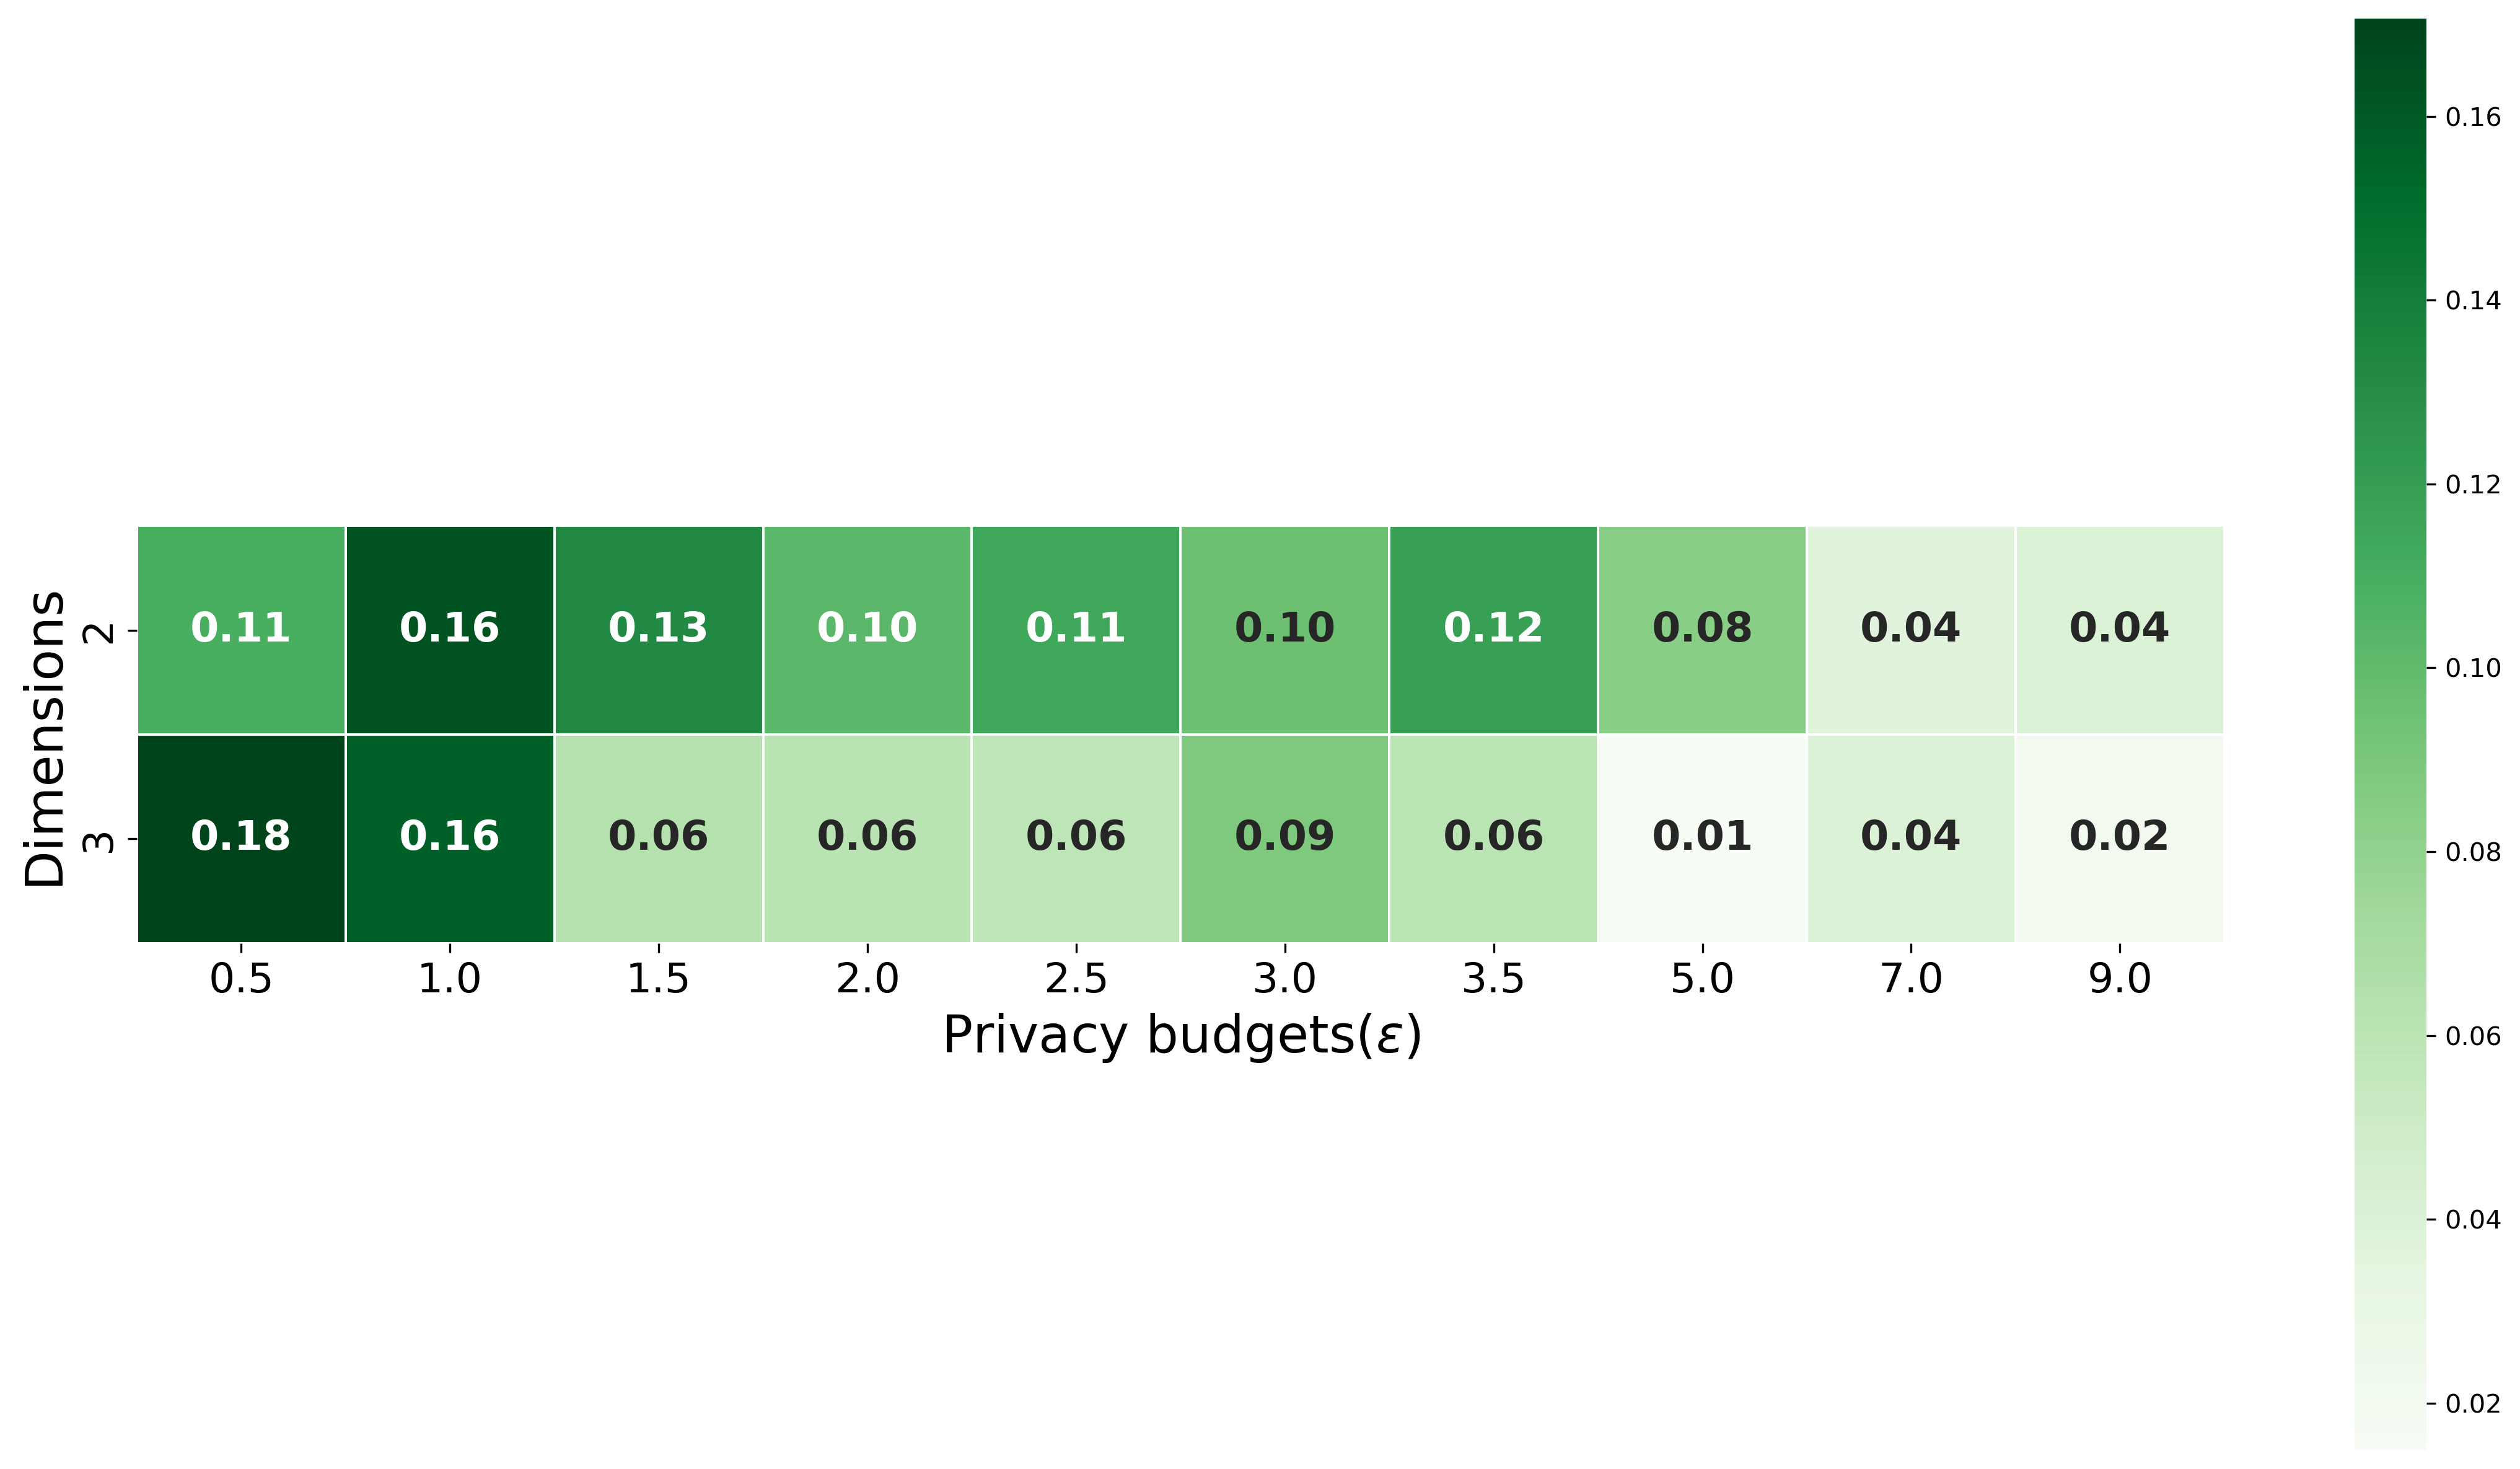
\includegraphics[width=1\textwidth]{Results/nd-laplace/nd-Laplace/line-dataset/shokri_mi_adv.png}
      \label{fig:privacy_line-dataset_adversial_advantage_kd-laplace}
    \end{subfigure}
    \vfill % vertical space

    \begin{subfigure}[c]{1\textwidth}
      \caption{\textbf{Heatmap showing adversary advantage for the Piecewise mechanism, per privacy budget \& dimension for seeds-dataset.}}
      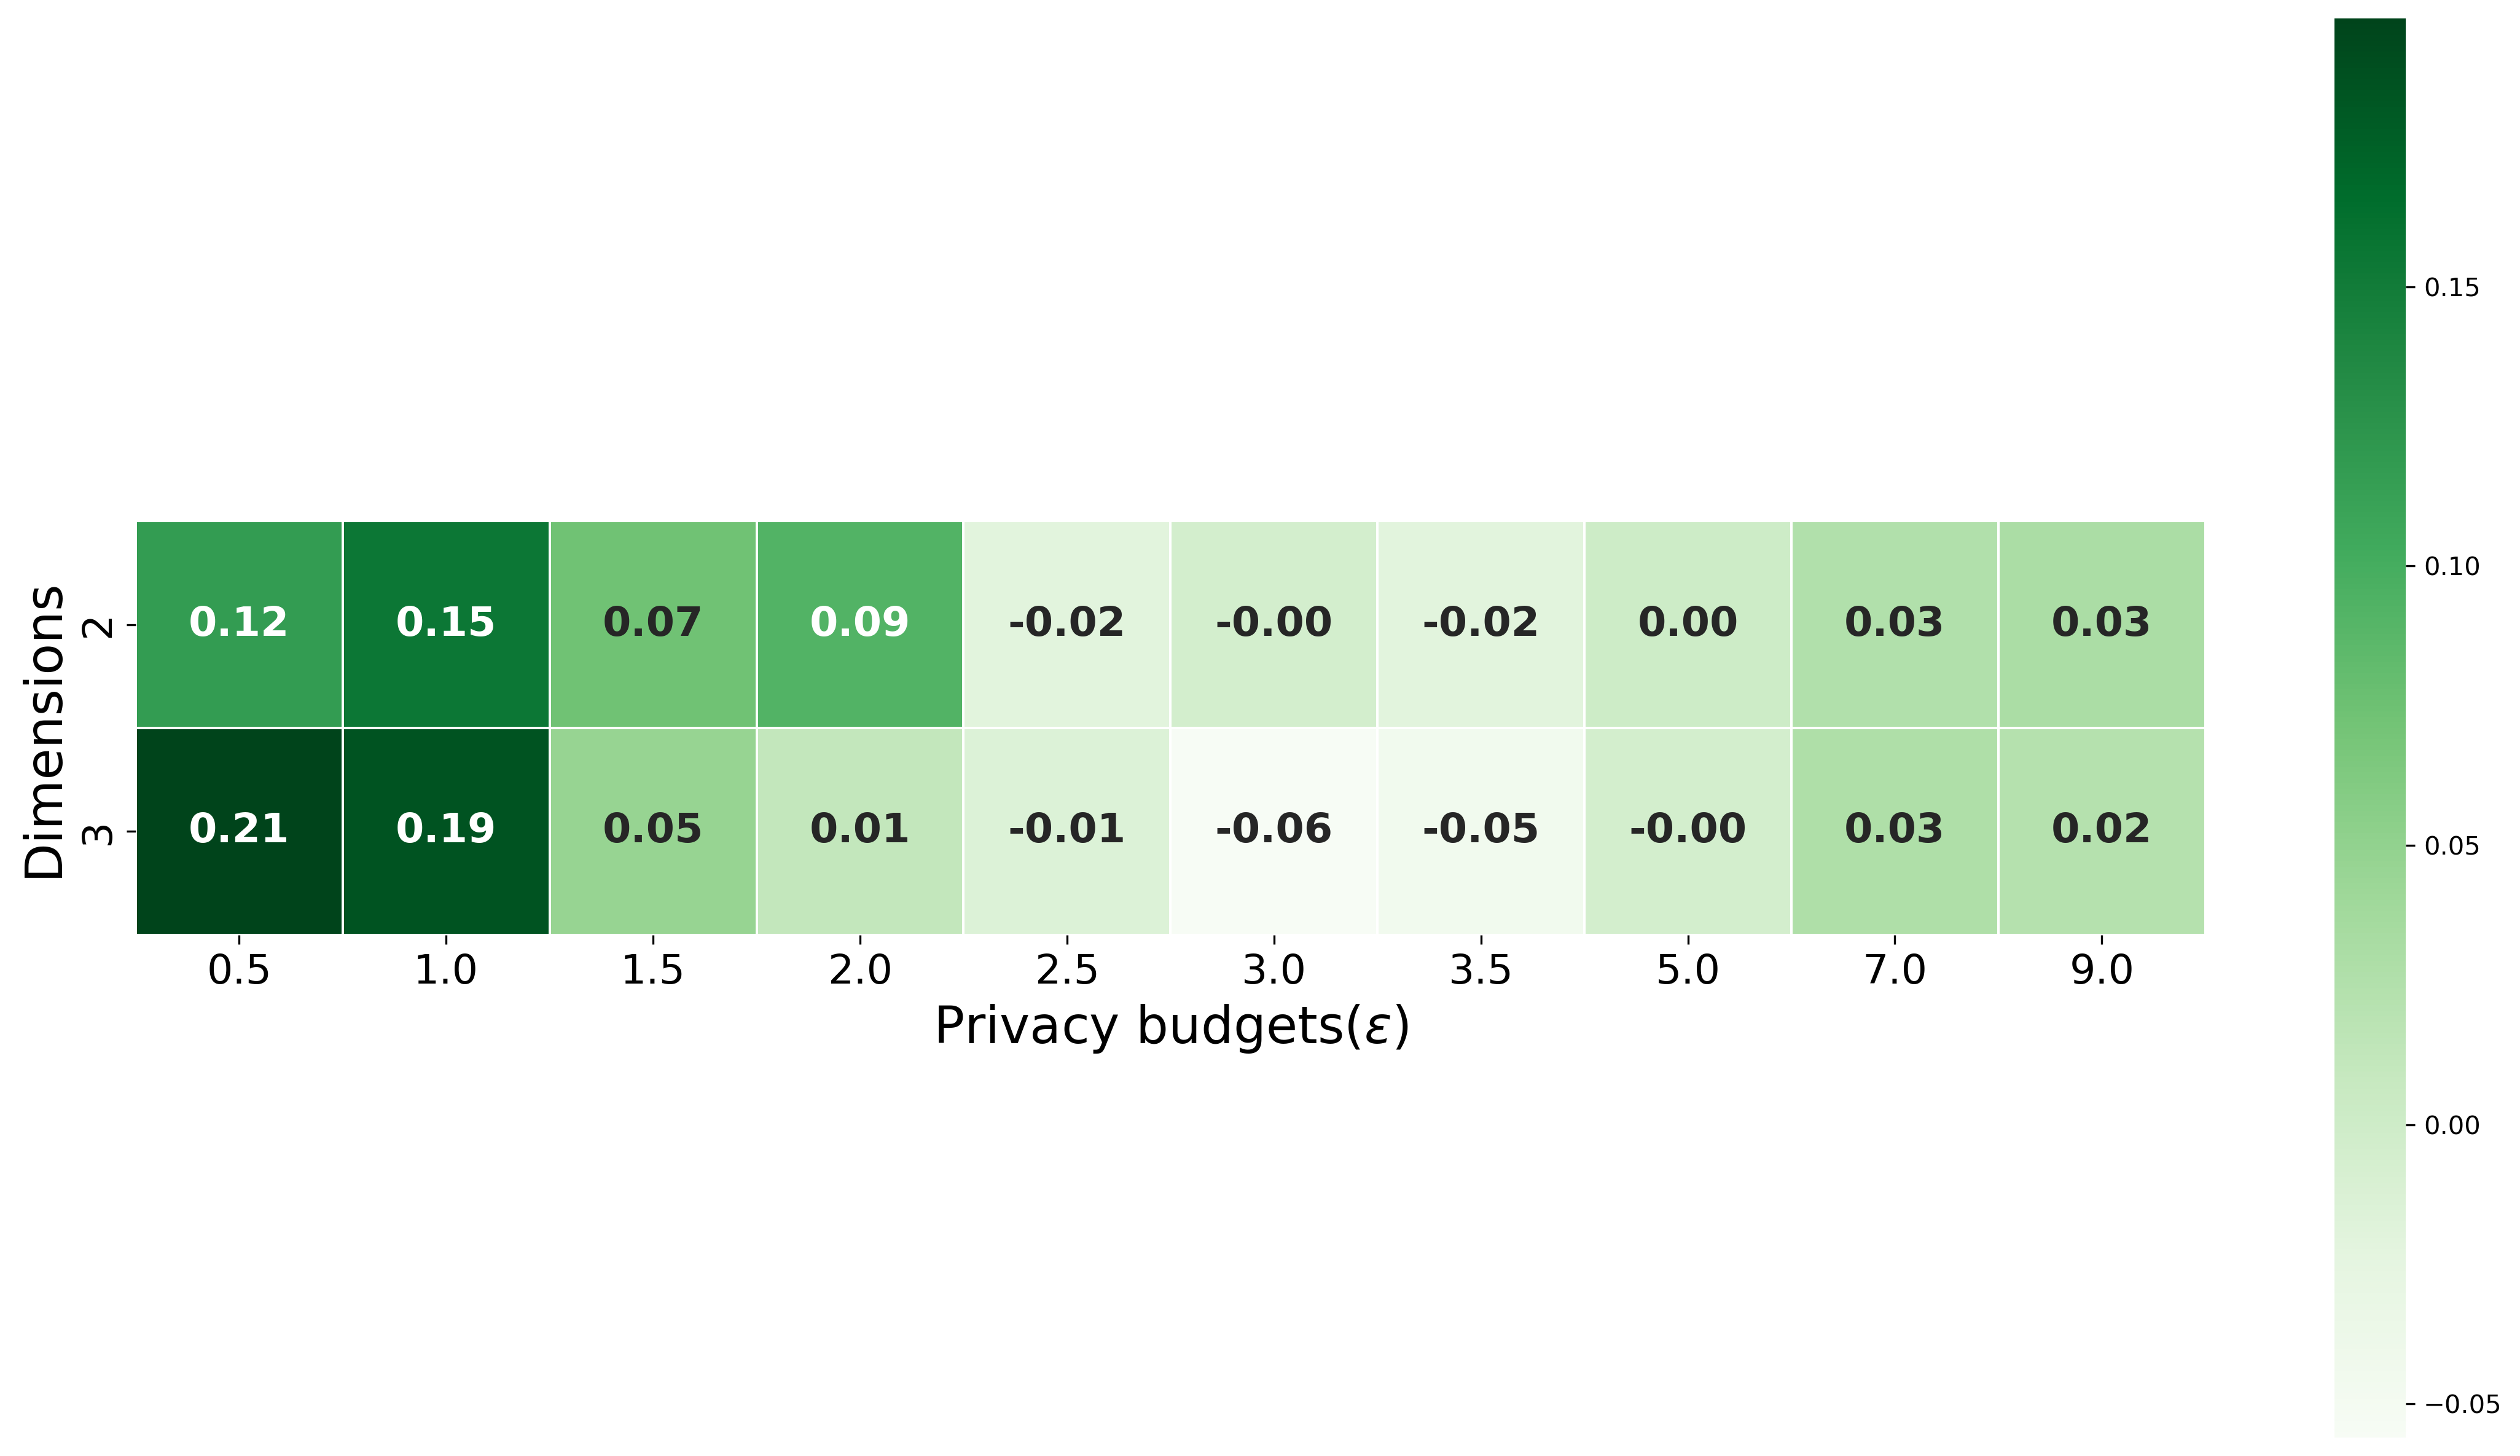
\includegraphics[width=1\textwidth]{Results/nd-laplace/piecewise/line-dataset/shokri_mi_adv.png}
      \label{fig:privacy_line-dataset_adversial_advantage_piecewise}
    \end{subfigure}
  \end{subfigure}
\end{figure}
\newpage
\subsection{Skewed dataset}
\begin{figure}[H]
  \centering
  \begin{subfigure}[b]{0.85\textwidth}
    \begin{subfigure}[c]{1\textwidth}
      \caption{\textbf{Heatmap showing adversary advantage for the kD-Laplace mechanism, per privacy budget \& dimension for seeds-dataset.}}
      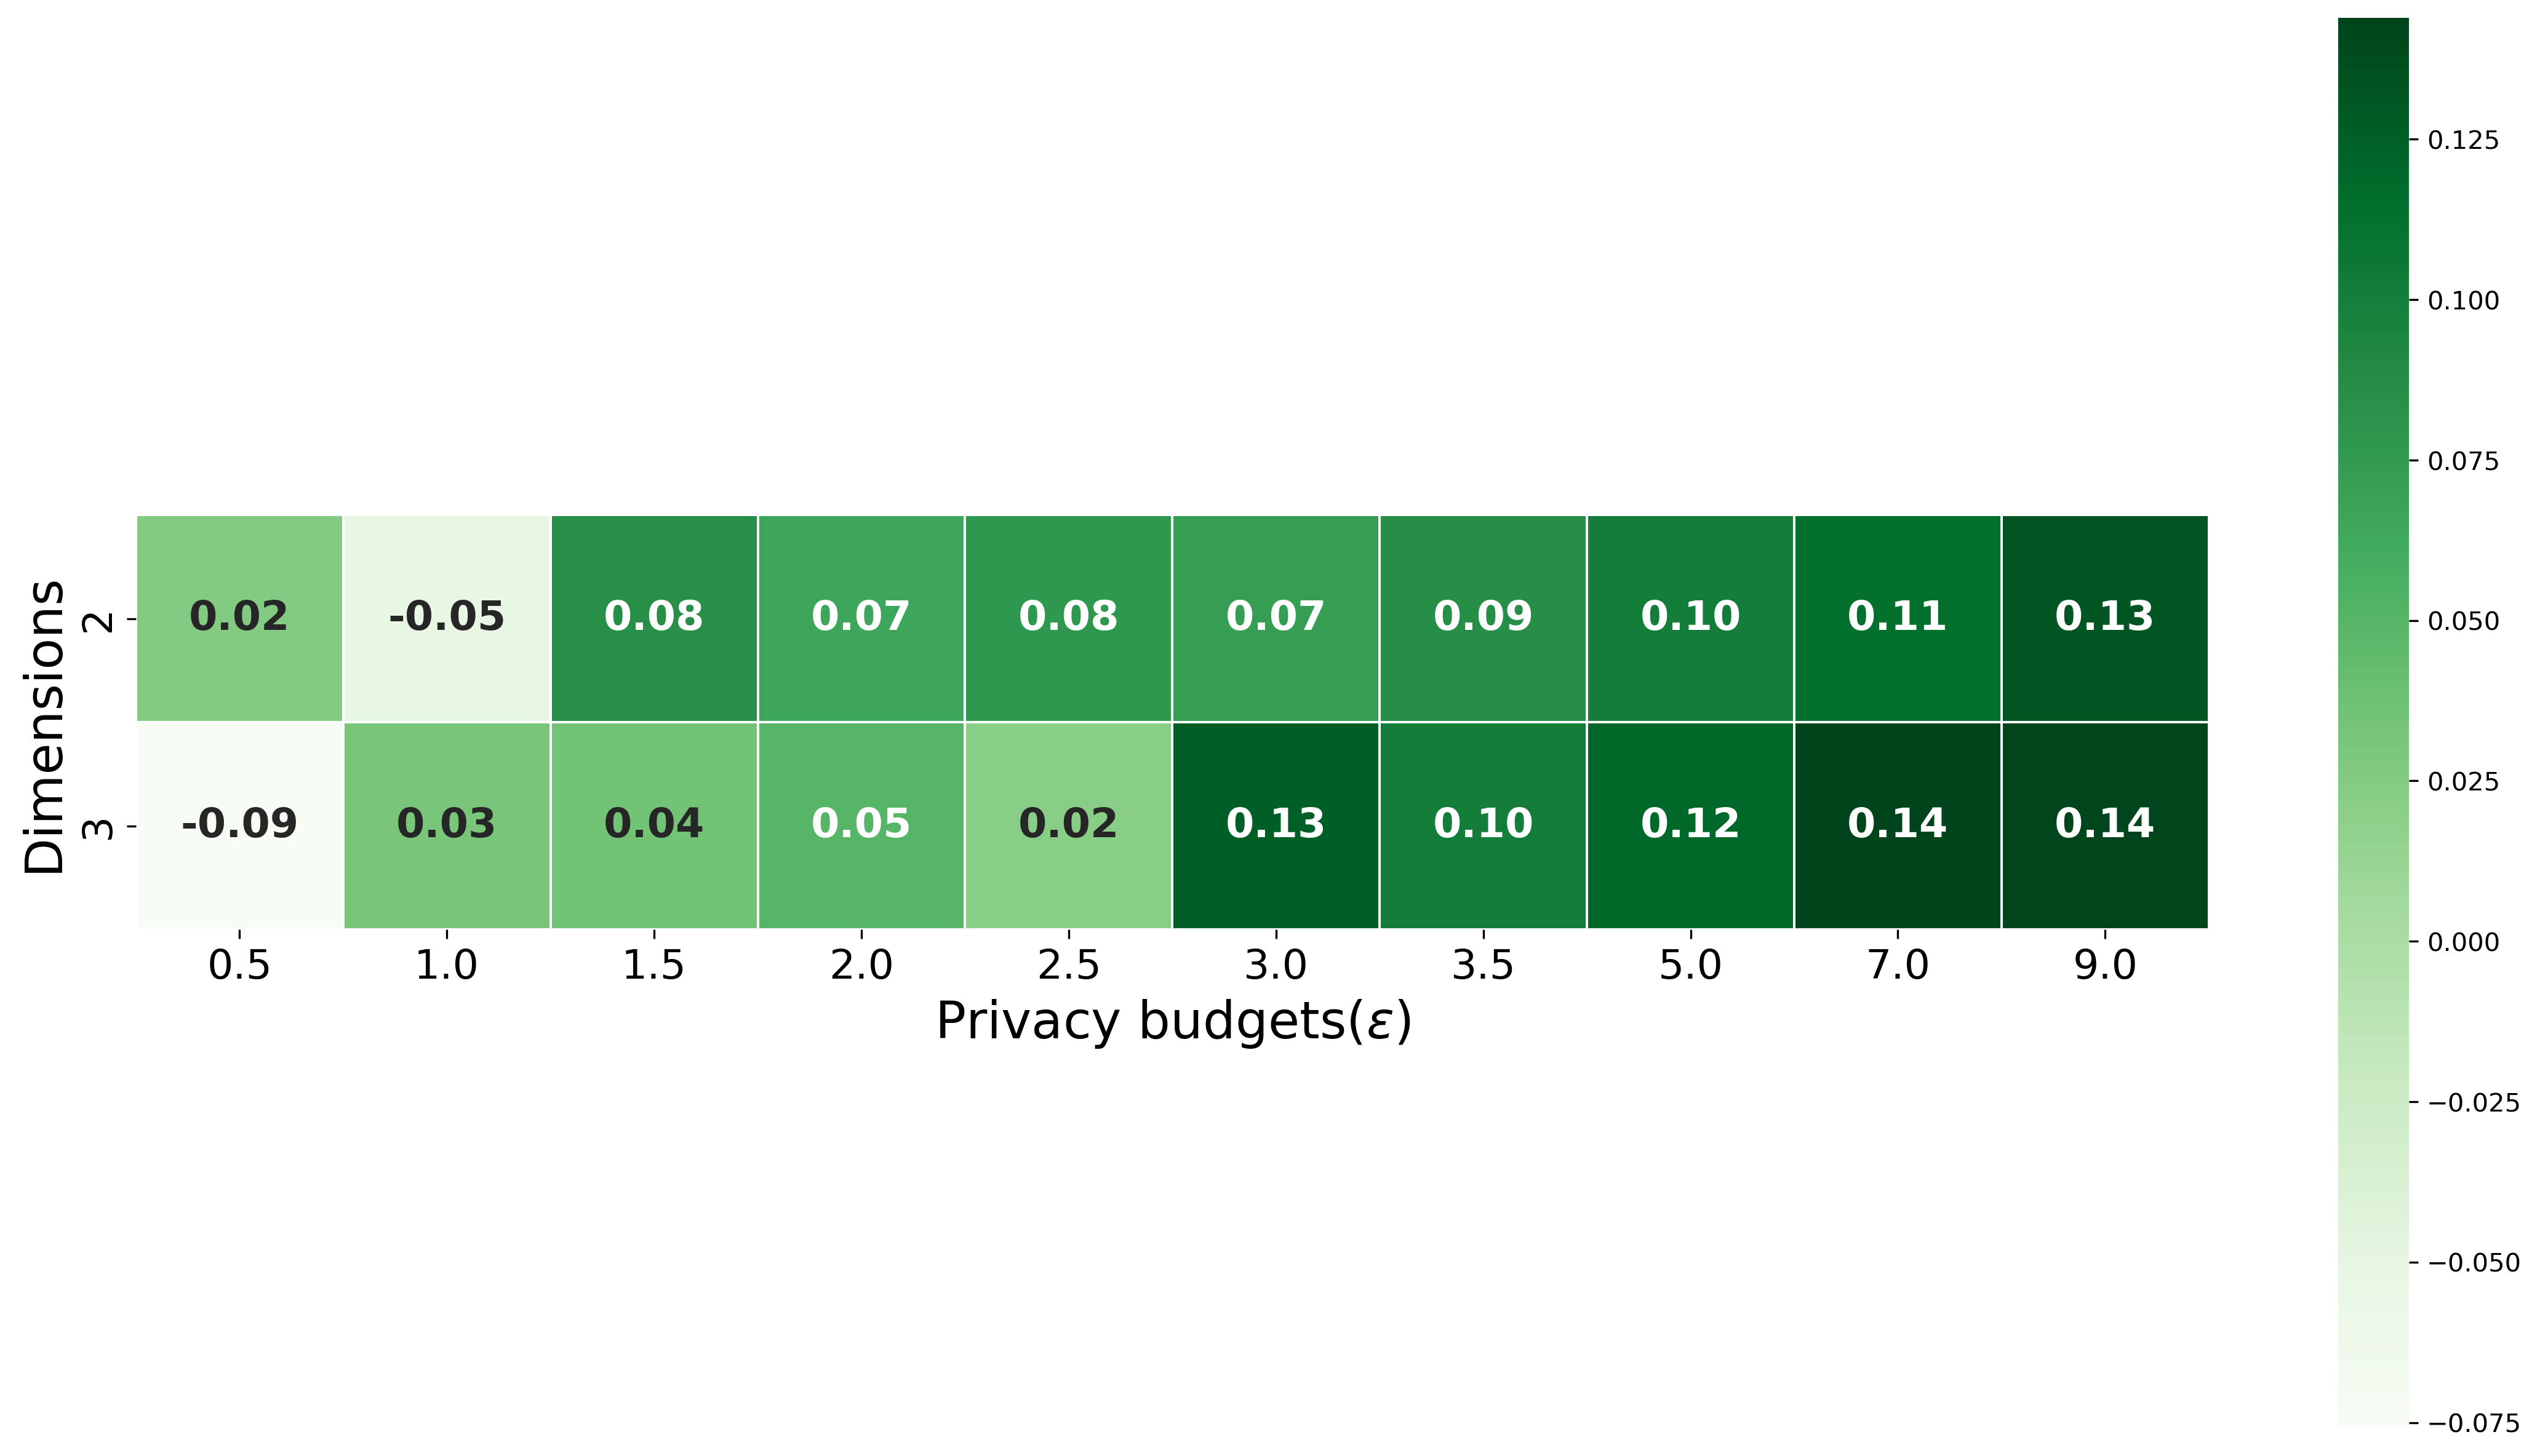
\includegraphics[width=1\textwidth]{Results/nd-laplace/nd-Laplace/skewed-dataset/shokri_mi_adv.png}
      \label{fig:privacy_skewed-dataset_adversial_advantage_kd-laplace}
    \end{subfigure}
    \vfill % vertical space

    \begin{subfigure}[c]{1\textwidth}
      \caption{\textbf{Heatmap showing adversary advantage for the Piecewise mechanism, per privacy budget \& dimension for seeds-dataset.}}
      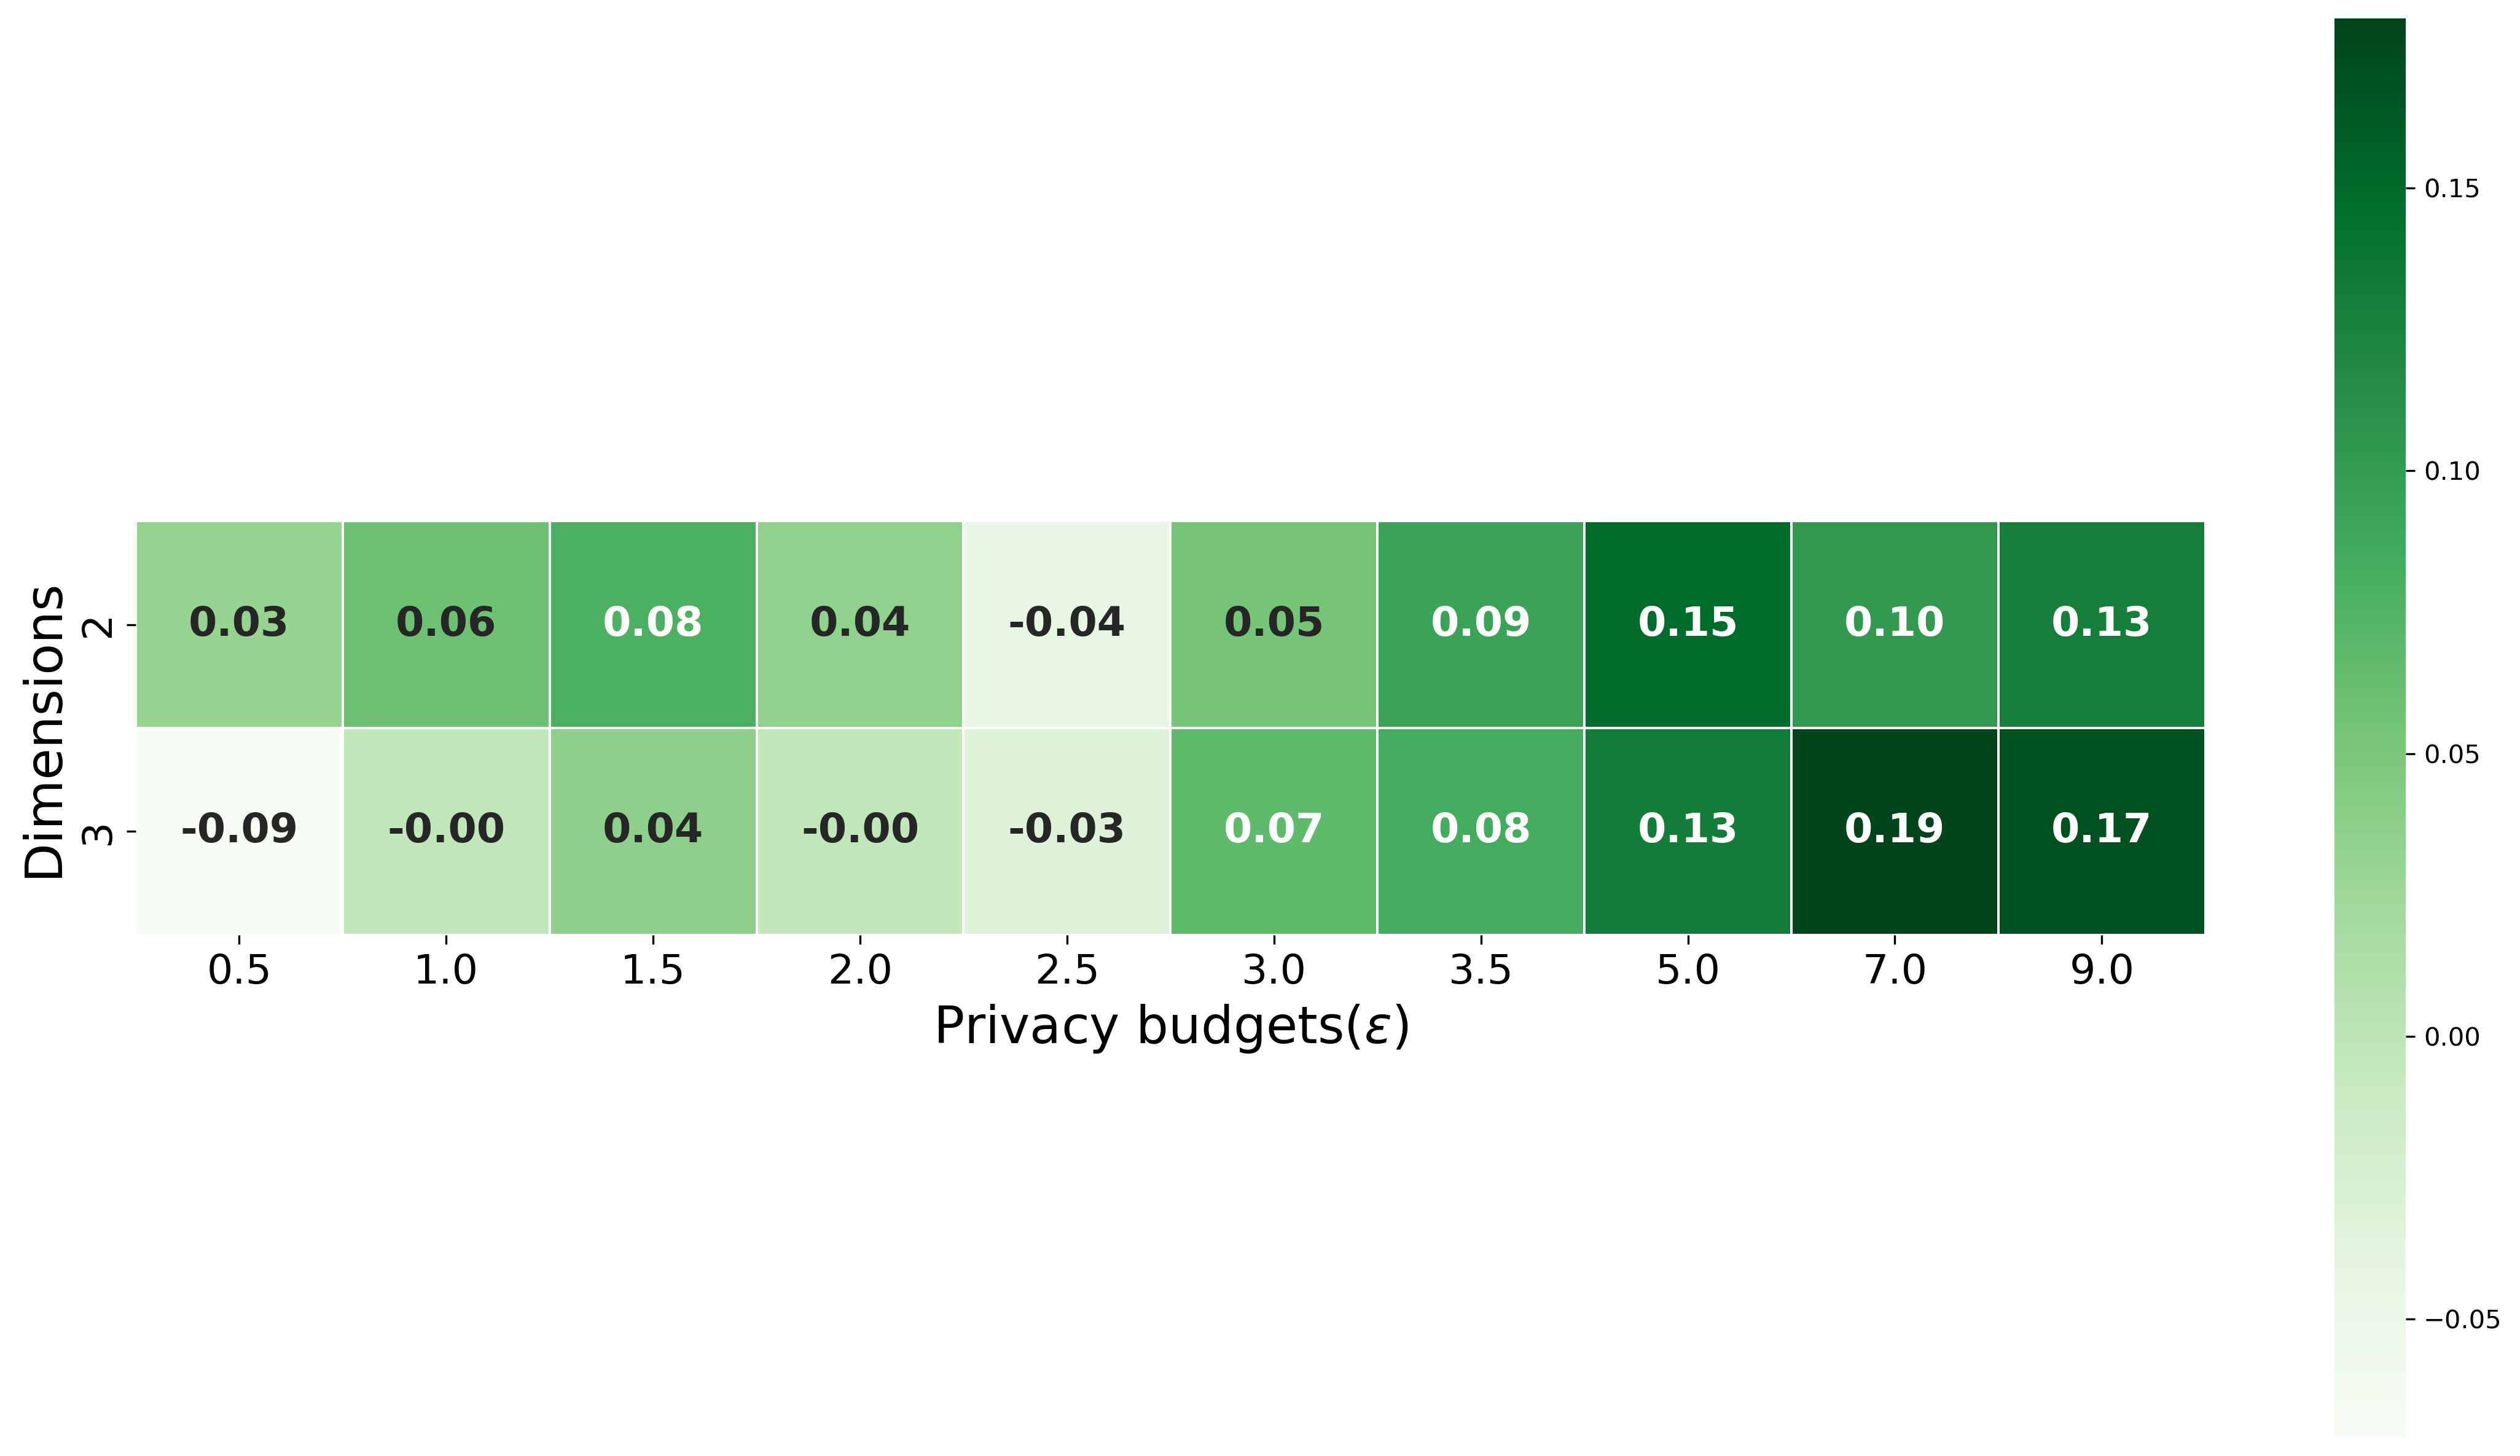
\includegraphics[width=1\textwidth]{Results/nd-laplace/piecewise/skewed-dataset/shokri_mi_adv.png}
      \label{fig:privacy_skewed-dataset_adversial_advantage_piecewise}
    \end{subfigure}
  \end{subfigure}
\end{figure}
\newpage
\subsection{Mechanism comparison}
In this section, we compare the different mechanisms for each dataset.
For this purpose, we also include all the different variants of kd-Laplace to see if there is a difference between them.
So, instead of comparing the mechanisms based on the number of dimensions, we compare them on the average scores for all dimensions per mechanism.
We are most interested in the utility and performance, and to compare them, we only show the \gls{ami} and adversary advantage scores.
\todo[inline]{Also needs privacy distance comparison}.
\begin{figure}[H]
  \centering
  \begin{subfigure}{0.30\textwidth}
    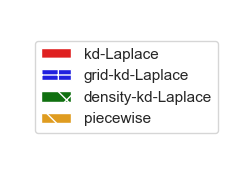
\includegraphics[width=\textwidth]{Results/kd-laplace/ami_bar_comparison_legend.png}
  \end{subfigure}
  \begin{subfigure}{1\textwidth}
    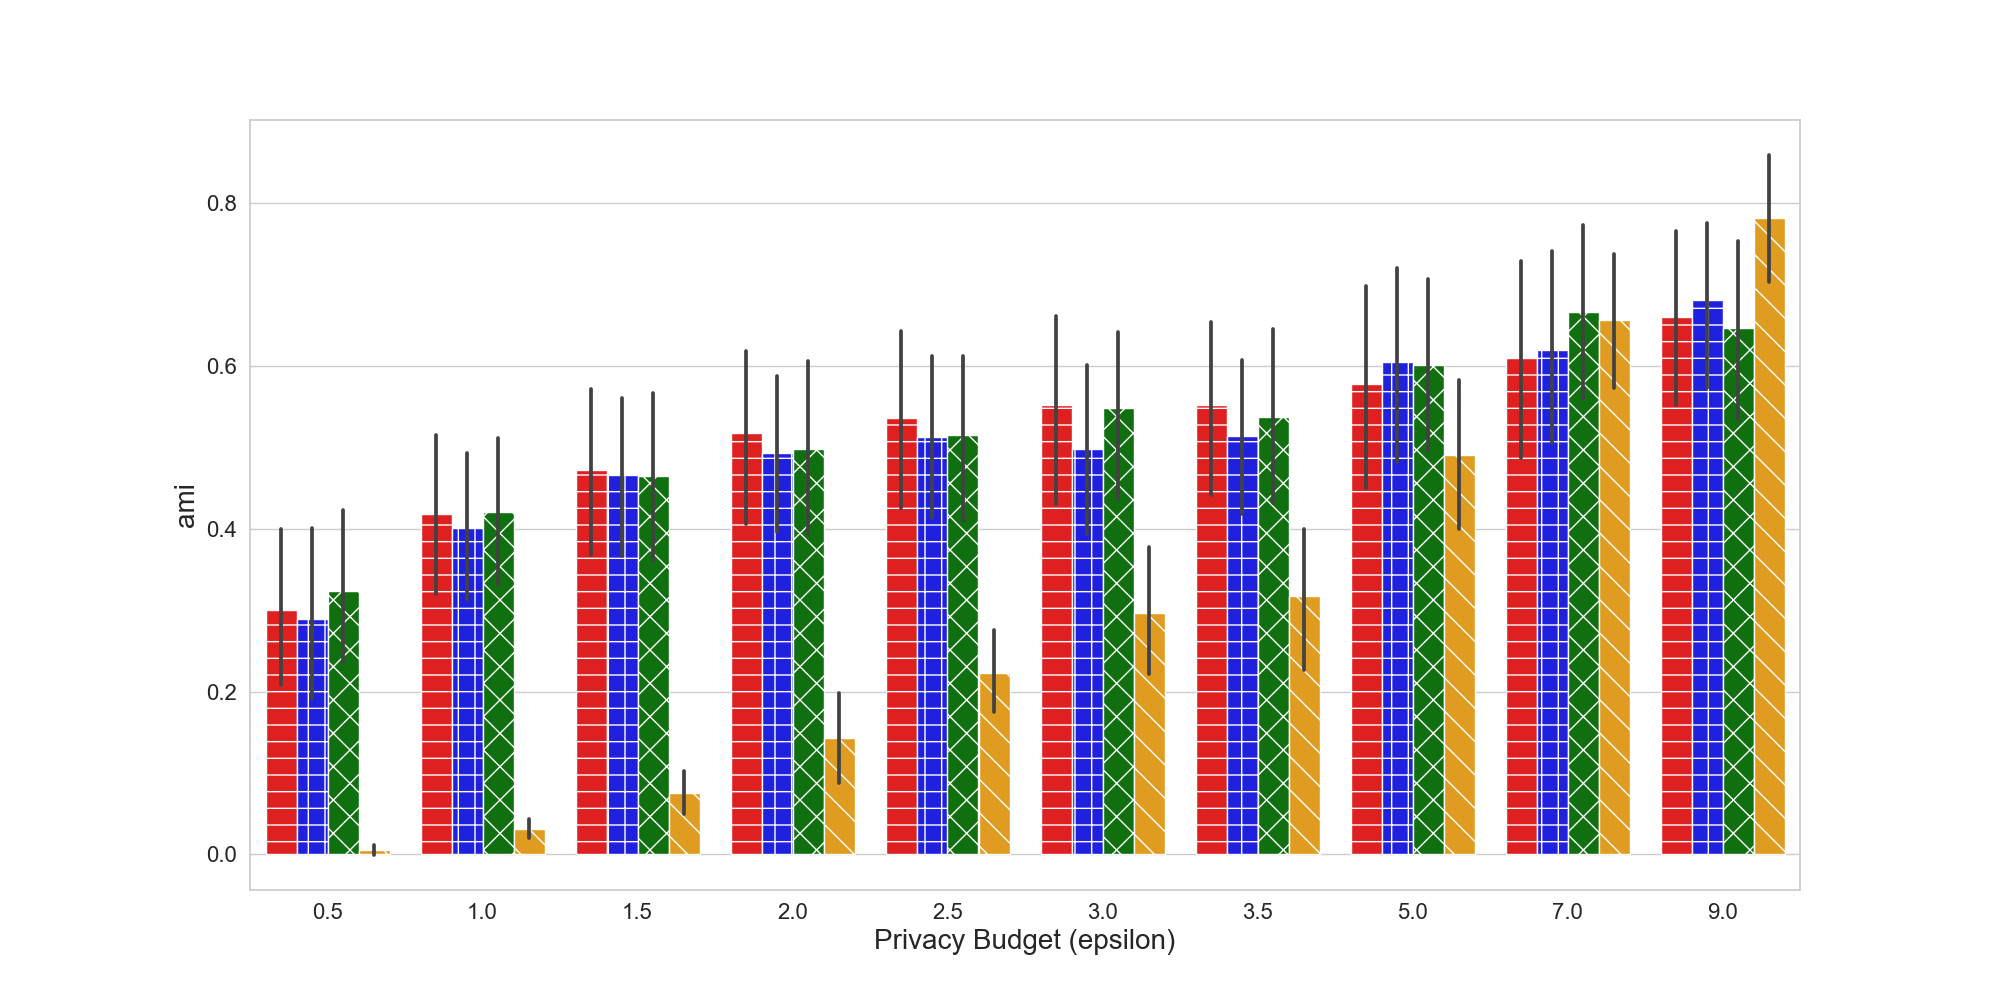
\includegraphics[width=1\textwidth]{Results/nd-laplace/ami_seeds-dataset_comparison.png}
  \end{subfigure}
  \begin{subfigure}{1\textwidth}
    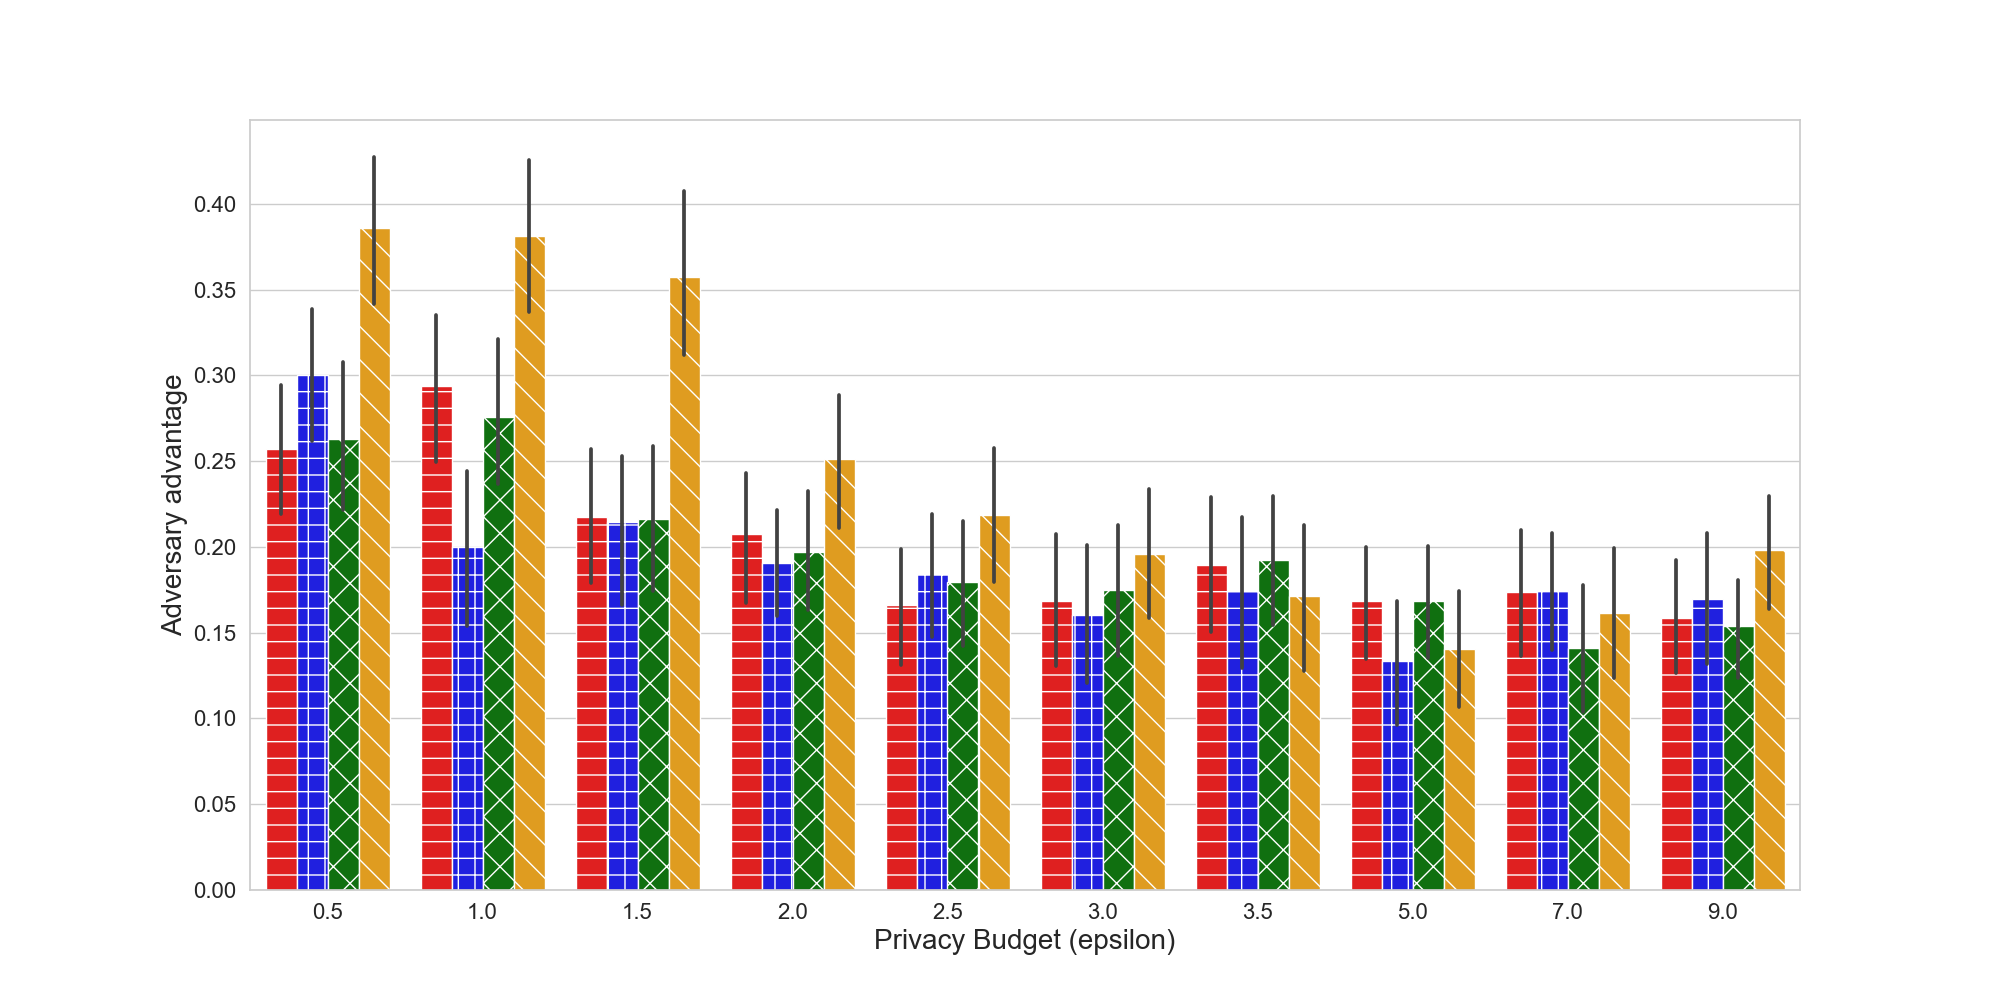
\includegraphics[width=1\textwidth]{Results/nd-laplace/shokri_mi_adv_seeds-dataset_comparison.png}
  \end{subfigure}
  \caption{Average AMI (top) and Adversary Advantage (bottom) comparison for each mechanism for seeds-dataset (8 dimensions).}
  \label{fig:utility_seeds-dataset_comparison_nd_plot}
\end{figure}
\todo[inline]{Add interpretation}
\newpage


\begin{figure}[H]
  \centering
  \begin{subfigure}{0.30\textwidth}
    \includegraphics[width=\textwidth]{Results/kd-laplace/ami_bar_comparison_legend.png}
  \end{subfigure}
  \begin{subfigure}{1\textwidth}
    \includegraphics[width=1\textwidth]{Results/nd-laplace/ami_heart-dataset_comparison.png}
  \end{subfigure}
  \begin{subfigure}{1\textwidth}
    \includegraphics[width=1\textwidth]{Results/nd-laplace/shokri_mi_adv_heart-dataset_comparison.png}
  \end{subfigure}
  \caption{Average AMI (top) and Adversary Advantage (bottom) comparison for each mechanism for heart-dataset (10 dimensions).}
  \label{fig:utility_heart-dataset_comparison_nd_plot}
\end{figure}
\todo[inline]{Add interpretation}
\newpage

\subsection{Shape datasets}

\begin{figure}[H]
  \centering
  \begin{subfigure}{0.30\textwidth}
    \includegraphics[width=\textwidth]{Results/kd-laplace/ami_bar_comparison_legend.png}
  \end{subfigure}
  \begin{subfigure}{1\textwidth}
    \includegraphics[width=1\textwidth]{Results/nd-laplace/ami_circle-dataset_comparison.png}
  \end{subfigure}
  \begin{subfigure}{1\textwidth}
    \includegraphics[width=1\textwidth]{Results/nd-laplace/shokri_mi_adv_circle-dataset_comparison.png}
  \end{subfigure}
  \caption{Average AMI (top) and Adversary Advantage (bottom) comparison for each mechanism for circle-dataset (3 dimensions).}
  \label{fig:utility_circle-dataset_comparison_nd_plot}
\end{figure}
\todo[inline]{Add interpretation}
\newpage

\begin{figure}[H]
  \centering
  \begin{subfigure}{0.30\textwidth}
    \includegraphics[width=\textwidth]{Results/kd-laplace/ami_bar_comparison_legend.png}
  \end{subfigure}
  \begin{subfigure}{1\textwidth}
    \includegraphics[width=1\textwidth]{Results/nd-laplace/ami_skewed-dataset_comparison.png}
  \end{subfigure}
  \begin{subfigure}{1\textwidth}
    \includegraphics[width=1\textwidth]{Results/nd-laplace/shokri_mi_adv_skewed-dataset_comparison.png}
  \end{subfigure}
  \caption{Average AMI (top) and Adversary Advantage (bottom) comparison for each mechanism for skewed-dataset (3 dimensions).}
  \label{fig:utility_skewed-dataset_comparison_nd_plot}
\end{figure}
\todo[inline]{Add interpretation}
\newpage



\begin{figure}[H]
  \centering
  \begin{subfigure}{0.30\textwidth}
    \includegraphics[width=\textwidth]{Results/kd-laplace/ami_bar_comparison_legend.png}
  \end{subfigure}
  \begin{subfigure}{1\textwidth}
    \includegraphics[width=1\textwidth]{Results/nd-laplace/ami_line-dataset_comparison.png}
  \end{subfigure}
  \begin{subfigure}{1\textwidth}
    \includegraphics[width=1\textwidth]{Results/nd-laplace/shokri_mi_adv_line-dataset_comparison.png}
  \end{subfigure}
  \caption{Average AMI (top) and Adversary Advantage (bottom) comparison for each mechanism for line-dataset (3 dimensions).}
  \label{fig:utility_line-dataset_comparison_nd_plot}
\end{figure}
\todo[inline]{Add interpretation}
\newpage



\mycomment{\subsection{3-dimensional data}
  \begin{figure}[H]
    \centering
    \begin{minipage}[c]{1.1\textwidth}
      \includegraphics[width=0.50\textwidth]{Results/RQ2/seeds-dataset/shokri_mi_adv_seeds-dataset_comparison.png}
      \includegraphics[width=0.50\textwidth]{Results/RQ2/seeds-dataset/tpr_seeds-dataset_comparison.png}
      \caption{Barplot for adversary advantage (left) and TPR (right) per privacy mechanism for seeds-dataset.}
      \label{fig:privacy_seeds-dataset_comparison_3d_aa_plot}
    \end{minipage}
    \begin{minipage}[c]{1.1\textwidth}
      \includegraphics[width=0.50\textwidth]{Results/RQ2/heart-dataset/shokri_mi_adv_heart-dataset_comparison.png}
      \includegraphics[width=0.50\textwidth]{Results/RQ2/heart-dataset/tpr_heart-dataset_comparison.png}
      \caption{Barplot for adversary advantage (left) and TPR (right) per privacy mechanism for heart-dataset.}
      \label{fig:privacy_heart-dataset_comparison_3d_aa_plot}
    \end{minipage}
  \end{figure}
  The graphs above show the adversary advantage (left) and TPR (right) for the seeds dataset (top) and heart dataset (bottom).
  The first dataset we analyze is the seeds dataset. We can observe a clear pattern for the Piecewise mechanism based on the adversary advantage plot for the seeds dataset. It scores between 0.4 and 0.5 for epsilon values ranging from 0.1 to 0.7 and drops below 0.2 for epsilon values higher than 3.
  The kd-Laplace mechanism, particularly the variant without optimizations (red), has a high adversary advantage (0.35) for epsilon 0.1. After that, all kd-Laplace variants perform similarly. When we compare them to the TPR, we still see that Piecewise and the regular kd-Laplace variant have higher scores for epsilon 0.1 (0.5+). After that, the mechanisms perform similarly, but we notice that kd-Laplace/grid/optimal consistently outperforms the others. Additionally, the latter is above the baseline value for epsilon 1.5.

  Now, let's turn our attention to the heart dataset. Here, we can see that the adversary advantage shows less variation than the seeds dataset. For all epsilon values, kd-Laplace without optimizations stands out. The mechanisms perform similarly, but the Piecewise mechanism performs better for epsilon values between 1.5 and 5.0.
  For the TPR, all mechanisms are below the baseline value. They score the same, but the Piecewise mechanism is approximately 0.05 TPR lower than the kd-Laplace variants for epsilon values 0.1 to 3.5.
  \newpage
  \begin{figure}[H]
    \centering
    \begin{minipage}[c]{1\textwidth}
      \includegraphics[width=1\textwidth]{Results/RQ2/seeds-dataset/privacy_distance_plot.png}
      \caption{Privacy distance for each mechanism for 3D seeds-dataset.}
      \label{fig:privacy_seeds-dataset_comparison_3d_privacy_distance_plot}
    \end{minipage}
    \begin{minipage}[c]{1\textwidth}
      \includegraphics[width=1\textwidth]{Results/RQ2/heart-dataset/privacy_distance_plot.png}
      \caption{Privacy distance for each mechanism for 3D heart-dataset.}
      \label{fig:privacy_heart-dataset_comparison_3d_privacy_distance_plot}
    \end{minipage}
  \end{figure}
  %#The above graphs depict the average Euclidean distances between the data with privacy mechanisms applied and without them for the seeds dataset (top) and heart dataset (bottom). 
  %A clear distinction can be observed among the different distances for the seeds dataset. On average, the Piecewise mechanism adds the most distance. 
  At epsilon values 7 and 9, the Piecewise mechanism adds the least distance. Among the various kd-Laplace variants, the variant without optimizations adds the most distance.
  This trend continues until epsilon 5, after which the variants become equal.

  Similarly, a noticeable difference is observed between the Piecewise mechanism and kd-Laplace for the heart dataset. At epsilon 9, the Piecewise mechanism has the same score as kd-Laplace.
  Among the kd-Laplace variants, the variant without optimizations adds the least distance, but it is slightly higher than the other variants for epsilon 0.1.
  \newpage
  %\subsection{Utility}
  %subsubsection*{Cluster comparison}
  %\todo[inline]{Add plot}
  %\subsubsection*{Mechanism comparison}
  %\begin{figure}[H]
  %    \includegraphics[width=\textwidth]{Results/RQ2/heart-dataset/ami_heart-dataset_comparison.png}
  %    \caption{Adjusted Mutual Information comparison for the 3-dimensional heart-dataset}
  %    \label{fig:ami_heart-dataset_comparison_3d}
  %\end{figure}
  %\begin{figure}[H]
  %    \includegraphics[width=\textwidth]{Results/RQ2/seeds-dataset/ami_seeds-dataset_comparison.png}
  %    \caption{Adjusted Mutual Information comparison for the 3-dimensional seeds-dataset}
  %    \label{fig:ami_seeds-dataset_comparison_3d}
  %\end{figure}
  %\todo[inline]{Add links to scilliouette plots and other plots}
  \subsection{n-dimensional data}
  \begin{figure}[H]
    \centering
    \begin{minipage}[c]{1.1\textwidth}
      \includegraphics[width=0.50\textwidth]{Results/RQ2-nd/seeds-dataset/shokri_mi_adv_seeds-dataset_comparison.png}
      \includegraphics[width=0.50\textwidth]{Results/RQ2-nd/seeds-dataset/tpr_seeds-dataset_comparison.png}
      \caption{Barplot for adversary advantage (left) and TPR (right) per privacy mechanism for seeds-dataset.}
      \label{fig:privacy_seeds-dataset_comparison_nd_aa_plot}
    \end{minipage}
    \begin{minipage}[c]{1.1\textwidth}
      \includegraphics[width=0.50\textwidth]{Results/RQ2-nd/heart-dataset/shokri_mi_adv_heart-dataset_comparison.png}
      \includegraphics[width=0.50\textwidth]{Results/RQ2-nd/heart-dataset/tpr_heart-dataset_comparison.png}
      \caption{Barplot for adversary advantage (left) and TPR (right) per privacy mechanism for heart-dataset.}
      \label{fig:privacy_heart-dataset_comparison_nd_aa_plot}
    \end{minipage}
  \end{figure}
  %The above graphs display the adversary advantage (left) and TPR (right) per epsilon for the seeds dataset (top) and heart dataset (bottom).

  The seeds dataset shows that Piecewise has a higher adversary advantage for epsilons ranging from 0.1 to 1.
  However, the TPR for Piecewise is consistently lower than that of kd-Laplace. There is no clear distinction among the kd-Laplace variants.
  However, for epsilon values 7 and 9, kd-Laplace/grid/optimal does not exceed the baseline for TPR, while the other variants do.

  For the heart dataset, the Piecewise mechanism scores below 0.10 for adversary advantage for epsilons 0.1 to 3.
  In contrast, the kd-Laplace variants yield values above 0.25 for the same epsilon values.
  The Piecewise mechanism also scores lower for epsilon values 3.5 and 5, but they have nearly equal scores for epsilons 7 and 9.
  Among the variants of kd-Laplace, kd-Laplace, and kd-Laplace/grid perform slightly worse for epsilon 0.1, but for the other epsilons, they function similarly.
  The TPR follows a similar trend to the adversary advantage, except for epsilon 0.1, where the kd-Laplace variants have equal scores.

  \newpage
  %\begin{tabular}{llrr}
\toprule
 &  & True Positive Rate & False Positive Rate \\
algorithm & epsilon &  &  \\
\midrule
\bottomrule
\end{tabular}


  \begin{figure}[H]
    \centering
    \begin{minipage}[c]{0.80\textwidth}
      \includegraphics[width=1\textwidth]{Results/RQ2-nd/seeds-dataset/privacy_distance_plot.png}
      \caption{Privacy distance for each mechanism for nD seeds-dataset.}
      \label{fig:privacy_seeds-dataset_comparison_nd_privacy_distance_plot}
    \end{minipage}
    \begin{minipage}[c]{0.80\textwidth}
      \includegraphics[width=1\textwidth]{Results/RQ2-nd/heart-dataset/privacy_distance_plot.png}
      \caption{Privacy distance for each mechanism for nD heart-dataset.}
      \label{fig:privacy_heart-dataset_comparison_nd_privacy_distance_plot}
    \end{minipage}
  \end{figure}
  The Piecewise mechanism for epsilon 0.1 to 3.5 for the seeds dataset adds the most Euclidean distance. After that, the Piecewise mechanism decreases significantly and scores lower than the kd-Laplace variants. For kd-Laplace/grid/optimal, the privacy distance starts lowest up to epsilon 1.5. After that, the variants of the kd-Laplace score are almost the same.

  For the heart dataset, the Piecewise mechanism also adds the most Euclidean distance, only now for all epsilons. The kd-Laplace/grid/optimal mechanism starts as the lowest again but is then the highest of all variants, and scores for epsilon 9 are almost equal to the Piecewise mechanism. The other two variants of kd-Laplace (grid / no optimization) score the same.

  \newpage
  \section{Dimensionality}
  The chart below provides two heat maps for the seeds dataset (top) and the heart dataset (bottom). The y-axis column represents the privacy budget (epsilon), and the x-axis represents the dimensions. In each cell of the matrix, the TPR (True Positive Rate) is indicated, so the darker the cell, the higher the TPR. A higher value implies that, on average, more information is leaked.
  \begin{figure}[H]
    \includegraphics[width=0.8\textwidth]{Results/RQ3/seeds-dataset/security_dimensions_heatmap_nd-laplace-optimal-truncated.png}
    \caption{Heatmap for TPR and dimensionality for the seeds-dataset for kd-Laplace/grid/optimal}
    \label{fig:security_dimensions_heatmap_seeds-dataset_comparison_nd-laplace-optimal-truncated}
    %\includegraphics[width=0.8\textwidth]{Results/RQ3/heart-dataset/security_dimensions_heatmap_nd-laplace-optimal-truncated.png}
    \caption{Heatmap for TPR and dimensionality for the heart-dataset for kd-Laplace/grid/optimal}
    \label{fig:security_dimensions_heatmap_hearts-dataset_comparison_nd-laplace-optimal-truncated}
  \end{figure}
  Generally, a higher epsilon value corresponds to a higher TPR for the seeds dataset. Dimensions 4 and 5 have the highest scores (0.60 >) starting from epsilon 5. The bottom row achieves the highest scores, and for dimensions 4, 5, and 6, TPR values less than 0.40 are reported for epsilon 0.1. No clear trend is visible for the remaining epsilon values based on increasing dimensions.

  The heart dataset's lowest scores (< 0.50) are also observed for epsilon 0.1 and dimensions 4 and 5. From epsilon 2 onwards, the values increase (> 0.50 TPR) for dimensions 4 and 5. The heatmap becomes darker for dimensions higher than 5, indicating TPR values higher than 0.60. From epsilon 6 and 8 dimensions, the scores exceed 0.70 TPR.
  \newpage

  \section{Shape}
  This chapter examines three datasets with a specific shape: circle, line, and left-skewed.
  The adversary advantages (privacy) and AMI (utility) are compared between the mechanisms for all three datasets.
  We compare kd-Laplace/grid/optimal (green) and Piecewise (yellow).
  \begin{figure}[H]
    \begin{minipage}[c]{0.55\textwidth}
      %\includegraphics[width=\textwidth]{Results/RQ3/circle-dataset/ami_circle-dataset_comparison.png}
    \end{minipage}
    \begin{minipage}[c]{0.55\textwidth}
      %\includegraphics[width=\textwidth]{Results/RQ3/circle-dataset/shokri_mi_adv_circle-dataset_comparison.png}
    \end{minipage}
    \label{fig:advantage_circle-dataset_comparison}
    \caption{The AMI (left) and adversary advantage (right) for the circle-dataset}
  \end{figure}
  There's a noticeable difference between the Piecewise and kd-Laplace/grid/optimal mechanisms in the circle dataset. For the AMI, Piecewise scores are significantly higher at epsilon 7 to 9. In comparison, kd-Laplace/grid/optimal scores are lower than 0.2 for most other epsilons. Regarding the adversary advantage, kd-Laplace/grid-optimal scores are lower than Piecewise, except for epsilon 1 and 1.5.
  \begin{figure}[H]
    \begin{minipage}[c]{0.55\textwidth}
      %\includegraphics[width=\textwidth]{Results/RQ3/line-dataset/ami_line-dataset_comparison.png}
    \end{minipage}
    \begin{minipage}[c]{0.55\textwidth}
      %\includegraphics[width=\textwidth]{Results/RQ3/line-dataset/shokri_mi_adv_line-dataset_comparison.png}
    \end{minipage}
    \label{fig:advantage_line-dataset_comparison}
    \caption{The AMI (left) and adversary advantage (right) for the line dataset}
  \end{figure}
  In the line dataset, Piecewise outperforms kd-Laplace/grid/optimal for epsilon values above 5 for the AMI metric. For epsilons between 0.1 and 5, kd-Laplace/grid/optimal scores are higher. Regarding adversary advantage, Piecewise performs worse for epsilons between 0.1 and 1.5, while kd-Laplace/grid/optimal scores worse for epsilons 2 to 7.
  \begin{figure}[H]
    \begin{minipage}[c]{0.55\textwidth}
      % \includegraphics[width=\textwidth]{Results/RQ3/skewed-dataset/ami_skewed-dataset_comparison.png}
    \end{minipage}
    \begin{minipage}[c]{0.55\textwidth}
      %\includegraphics[width=\textwidth]{Results/RQ3/skewed-dataset/shokri_mi_adv_skewed-dataset_comparison.png}
    \end{minipage}
    \label{fig:advantage_skewed-dataset_comparison}
    \caption{The AMI (left) and adversary advantage (right) for the skewed dataset}

  \end{figure}
  Kd-Laplace/grid/optimal is better than Piecewise for skewed datasets, across all epsilon values, with AMI scores ranging from 0.6 to 0.8. For adversary advantage, Kd-Laplace/grid/optimal outperforms Piecewise between 0.1 and 1.0 epsilon values. The adversary advantage stays low for both mechanisms (below 0.1).
}
\newpage
\chapter*{Conclusion}
\todo[inline]{In progress}
\newpage
\chapter{Discussion}
For each result we added an interpretation and discussion section. This section summarizes these findings and also provides a list of future research directions.

In our research, we applied many different experiments to determine the utility and privacy characteristics of the nD-Laplace mechanism compared to the Piecewise mechanism. For this, we used five different datasets, including two real-world datasets: seeds-dataset and heart-dataset. Additionally, we generated three synthetic datasets (Circle, Line and Skewed) to see how nD-Laplace deals with them.

The initial research was conducted for the utility of three clustering algorithms: K-Means, \gls{ag}, and \gls{optics}. Subsequent experiments were conducted to identify the differences between the Piecewise mechanism and nD-Laplace. First in terms of utility, where both internal (\gls{sc}) and external (\gls{ami}) validation was performed. Similarly, research was conducted into privacy, mainly looking at membership advantage and \gls{tpr}.
Finally, an experiment was conducted to also include the variants of nD-Laplace in the comparison, looking at the same metrics. \newline

Using Jupyter notebook, the research can be reproduced. 
Additionally, a version control system (git) was used, and all datasets were stored in it, ensuring no external changes occurred that could influence the results.
Lastly, the results are robust because they were all repeated 10 times, and the average was taken. \newline

From our results, it has become evident that the privacy budget has a clear impact on the utility and privacy of nD-Laplace.
As the privacy budget increases, the utility goes up, but privacy decreases.
This aligns with what we have seen in the literature \citep{sun_distributed_2019, xia_distributed_2020, 9679364}. 

When comparing the utility of the nD-Laplace mechanism to the Piecewise mechanism, clear results emerge. The nD-Laplace mechanism performs well for the heart-dataset, seeds-dataset, and skewed dataset. Especially the K-Means and \gls{ag} clustering \gls{ami} scores are very high compared to the Piecewise mechanism. On the other hand, nD-Laplace did not score well on the line-dataset and circle dataset.
Also, we did not expect \gls{optics} to show such a low score for \gls{ami}. \newline

The dimensions showed minimal impact on the utility and privacy of the seeds and heart-dataset.
For these datasets, the most notable result was achieved for the highest two dimensions as these show a slight increase in \gls{ami}. This indicates a higher utility is achieved for more dimensions. \todo[inline]{Research literature}. This did impact the membership advantage, but when we considered the \gls{tpr} no specific change was visible. This indicates that although the utility increases for the highest two dimensions, the privacy does not. 

In conclusion, we conducted experiments to analyze the variants of nD-Laplace. These variants are named grid-nD-Laplace and density-nD-Laplace, both primarily aiming to ensure that the data from nD-Laplace remains within the original domain. 
From the literature, we had already determined that a remapping/truncation method is essential. Otherwise, with a low epsilon, the data is plotted outside the original domain, making it easy for an attacker to determine whether the data belongs to the original set or not.
Our experiments confirmed this, as a low privacy budget reported a much lower membership advantage. This was expected, but not to such an extent (lower than -50). 
Upon further investigation, this turned out to be a misrepresentation by the membership advantage metric, as identified as one of the shortcomings of the metric in the literature review \todo{citation}. The underlying \gls{tpr} was much higher, which is not the pattern we would expect for a lower privacy budget.
Since this does not occur (or to a lesser extent) with the variants of nD-Laplace, it can be attributed to the fact that the data for epsilon 0.5 is plotted far outside the original data domain. 
Of the two variants, grid-remapping seems to handle this best. We also observe that this variant consistently falls below the baseline value of the membership advantage, while its utility is not less than that of nD-Laplace.

For the density-nD-Laplace mechanism, we expected it to reduce the impact of data shape. However, in practice, this does not seem to work, and we do not see a consistent improvement in utility or privacy compared to the nD-Laplace mechanism. \newline

\subsection{Constraints}
Our research proved some difficulties with the \gls{optics} clustering algorithm.
Based on our research we saw a significant amount of clusters (15 - 19) in comparison to K-Means and \gls{ag}, which 2 to 9 clusters. In addition, the amount of points that were reported as noise was also around 40 - 50\%, while normally this is around 1 - 30\% \citep{schubert_dbscan_2017}. This indicates the number of $minPts$ might be to low, so the \gls{optics} is not be-able to find close-by points. This influences the performance of \gls{optics}, which makes it for this research hard to evaluate the proper scoring. However, it is still clear that Piecewise scores better for this cluster algorithm, even with incorrect clustering. This is the way Piecewise is be-able to handle to preserve difficult shapes, for example the line and seeds-dataset shapes (See Figure \ref{fig:evaluate-optics-seeds-dataset-2d-9eps} and Figure \ref{fig:validation-Line-dataset_comparison_2d-laplace}).

\subsection{Future work}
The results for nD-Laplace suggest a promising future for its application in clustering capabilities. More research is needed, but based on the current results, the algorithm shows clear strengths and weaknesses compared to the state-of-the-art Piecewise mechanism. 
However, the nD-Laplace mechanism still has a way to go when it comes to practical applications. This is primarily due to the limitation of nD-Laplace in not being able to work with certain data forms. Additionally, there are other areas where the nD-Laplace mechanism can be improved to broaden its practical applicability.
Therefore, we have compiled a list of ideas for follow-up work:

\begin{enumerate}
    \item \textbf{Research different data-shapes}:  This is an important issue for future research. Because nD-Laplace is not practical viable, if it cannot corporate with different shapes. While the Piecewise mechanism is consistent for most datasets, we see a strong distortion for nD-Laplace with datasets like Circle and Line. 
These datasets require a directed noise, instead of a uniform distribution of noise. Therefore, further research has to be conducted to reduce the impact of these datasets.
\item \textbf{Research dimensions on shape datasets: } The research we conducted is limited by 7 and 9 dimensions for the seeds-dataset and heart-dataset. However, we did not consider any dimensions higher then 3 for the synthetic datasets. Further research should be undertaken to explore how the dimensions have impact on these datasets. 
\item \textbf{Higher dimensions}: The research for dimensions capped at 9 dimensions. After 7, we saw a slight correlation with an improved utility. Therefore, further research should focus on higher dimensional data (20+ dimensions). 
\item \textbf{Categorical and binary data}: The Piecewise mechanism already does this, and it would be a good step to enhance the practical application scope of nD-Laplace. Future research can therefore focus on supporting categorical and binary data.
\end{enumerate}



%\input{Chapter2/chapter-2}

%\input{Chapter3/chapter-3}

%\input{Chapter4/chapter-4}

%\input{Chapter5/chapter-5}

%\input{Chapter6/chapter-6}



\backmatter
\pagenumbering{roman}

\bibliographystyle{plainnat}
\bibliography{report}

%% Use letters for the chapter numbers of the appendices.
%\appendix

%  \chapter{Hyperparameters}
\section{K-Means}
For selecting the appropriate amount of clusters, we used the silhouette method. 
Using this method, we ran the K-Means method multiple times for different $k$ values.
The results are plotted using a line-plot, and we select the highest silhouette score from this plot. 
\begin{enumerate}
  \item Seeds dataset (All dimensions): k-clusters.
  \begin{enumerate}
      \item 2-dimensions k-value: 2
      \item 3-dimensions k-value: 5
      \item 7-dimensions k-value: 2
  \end{enumerate}
      \item Heart dataset:
      \begin{enumerate}
          \item 2-dimensions k-value: 2
          \item 3-dimensions k-value: 4
          \item 9-dimensions k-value: 2
      \end{enumerate}
      \item Circle dataset:
      \begin{enumerate}
          \item 2-dimensions k-value: 7
          \item 3-dimensions k-value: 9
      \end{enumerate}
      \item Line dataset:
      \begin{enumerate}
          \item 2-dimensions k-value: 2
          \item 3-dimensions k-value: 2
      \end{enumerate}
      \item Skewed dataset:
      \begin{enumerate}
          \item 2-dimensions k-value: 5
          \item 3-dimensions k-value: 4
      \end{enumerate}
  \end{enumerate}

\newpage
\subsection{Seeds dataset}
\begin{figure}[H]
  \includegraphics[width=0.75\textwidth]{Method/images//k-values/seeds-dataset-2-kmeans.png}
  \caption{Selecting the $k$ for K-Means clustering for seeds dataset (2 dimensions) using the "silhouette method"}
  \label{hyperparameters:agglomerative-seeds-dataset-2d}
\end{figure}
\begin{figure}[H]
  \includegraphics[width=0.75\textwidth]{Method/images/k-values/seeds-dataset-2-kmeans.png}
  \caption{Selecting the $k$ for K-Means clustering for seeds dataset (3 dimensions) using the "silhouette method"}
  \label{hyperparameters:agglomerative-seeds-dataset-3d}
\end{figure}
\begin{figure}[H]
  \includegraphics[width=0.75\textwidth]{Method/images/k-values/seeds-dataset-n-kmeans.png}
  \caption{Selecting the $k$ for K-Means clustering for seeds dataset (7 dimensions) using the "silhouette method"}
  \label{hyperparameters:agglomerative-seeds-dataset-7d}
\end{figure}
\newpage

\subsection{Heart dataset}
\begin{figure}[H]
  \includegraphics[width=0.75\textwidth]{Method/images/k-values/heart-dataset-2-kmeans.png}
  \caption{Selecting the $k$ for K-Means clustering for Heart dataset (2 dimensions) using the "silhouette method"}
  \label{hyperparameters:agglomerative-heart-dataset-2d}
\end{figure}
\begin{figure}[H]
  \includegraphics[width=0.75\textwidth]{Method/images/k-values/heart-dataset-3-kmeans.png}
  \caption{Selecting the $k$ for K-Means clustering for Heart dataset (3 dimensions) using the "silhouette method"}
  \label{hyperparameters:agglomerative-heart-dataset-3d}
\end{figure}
\begin{figure}[H]
  \includegraphics[width=0.75\textwidth]{Method/images/k-values/heart-dataset-n-kmeans.png}
  \caption{Selecting the $k$ for K-Means clustering for Heart dataset (9 dimensions) using the "silhouette method"}
  \label{hyperparameters:agglomerative-heart-dataset-9d}
\end{figure}
\newpage

\subsection{Circle dataset}

\begin{figure}[H]
  \includegraphics[width=0.75\textwidth]{Method/images/k-values/circle-dataset-2-kmeans.png}
  \caption{Selecting the $k$ for K-Means clustering for circle dataset (2-dimensions) using the "silhouette method"}
  \label{hyperparameters:agglomerative-circle-dataset-2d}
\end{figure}
\begin{figure}[H]
  \includegraphics[width=0.75\textwidth]{Method/images/k-values/circle-dataset-3-kmeans.png}
  \caption{Selecting the $k$ for K-Means clustering for circle dataset (3-dimensions) using the "silhouette method"}
  \label{hyperparameters:agglomerative-circle-dataset-3d}
\end{figure}
\newpage

\subsection{Line dataset}
\begin{figure}[H]
  \includegraphics[width=0.75\textwidth]{Method/images/k-values/line-dataset-2-kmeans.png}
  \caption{Selecting the $k$ for K-Means clustering for line dataset (2-dimensions) using the "silhouette method"}
  \label{hyperparameters:agglomerative-line-dataset-2d}
\end{figure}
\begin{figure}[H]
  \includegraphics[width=0.75\textwidth]{Method/images/k-values/line-dataset-3-kmeans.png}
  \caption{Selecting the $k$ for K-Means clustering for line dataset (3-dimensions) using the "silhouette method"}
  \label{hyperparameters:agglomerative-line-dataset-3d}
\end{figure}
\newpage
\subsection{Skewed dataset}
\begin{figure}[H]
  \includegraphics[width=0.75\textwidth]{Method/images/k-values/skewed-dataset-2-kmeans.png}
  \caption{Selecting the $k$ for K-Means clustering for skewed dataset (2-dimensions) using the "silhouette method"}
  \label{hyperparameters:agglomerative-skewed-dataset-2d}
\end{figure}
\begin{figure}[H]
  \includegraphics[width=0.75\textwidth]{Method/images/k-values/skewed-dataset-3-kmeans.png}
  \caption{Selecting the $k$ for K-Means clustering for skewed dataset (3-dimensions) using the "silhouette method"}
  \label{hyperparameters:agglomerative-skewed-dataset-3d}
\end{figure}
\newpage
\section{Agglomerative clustering} \label{appendix:agglomerative-hyperparameters}
The same as with K-Means applies to \gls{ag}.
\begin{enumerate}
    \item Seeds dataset:
    \begin{enumerate}
        \item 2-dimensions k-value: 2
        \item 3-dimensions k-value: 2
        \item 7-dimensions k-value 4
    \end{enumerate}
    \item     Heart dataset:
    \begin{enumerate}
        \item 2-dimensions k-value: 2
        \item 3-dimensions k-value: 4
        \item 9-dimensions k-value 3
    \end{enumerate}
    \item Circle dataset:
    \begin{enumerate}
        \item 2-dimensions k-value: 7
        \item 3-dimensions k-value: 9
    \end{enumerate}
    \item Line dataset (all dimensions) k-value: 
    \begin{enumerate}
        \item 2-dimensions k-value: 2
        \item 3-dimensions k-value: 3
    \end{enumerate}
    \item Skewed dataset:
    \begin{enumerate}
        \item 2-dimensions k-value: 6
        \item 3-dimensions k-value: 9
    \end{enumerate}
\end{enumerate}
\newpage
\subsection{Seeds dataset}
\begin{figure}[H]
  \includegraphics[width=0.75\textwidth]{Method/images/k-values/seeds-dataset-2-agglomerative.png}
  \caption{Selecting the $k$ for Agglomerative clustering for seeds dataset (2 dimensions) using the"silhouette method"}
  \label{hyperparameters:agglomerative-seeds-dataset-2d}
\end{figure}
\begin{figure}[H]
  \includegraphics[width=0.75\textwidth]{Method/images/k-values/seeds-dataset-3-agglomerative.png}
  \caption{Selecting the $k$ for Agglomerative clustering for seeds dataset (3 dimensions) using the "silhouette method"}
  \label{hyperparameters:agglomerative-seeds-dataset-3d}
\end{figure}
\begin{figure}[H]
  \includegraphics[width=0.75\textwidth]{Method/images/k-values/seeds-dataset-n-agglomerative.png}
  \caption{Selecting the $k$ for Agglomerative clustering for seeds dataset (7 dimensions) using the "silhouette method"}
  \label{hyperparameters:agglomerative-seeds-dataset-7d}
\end{figure}
\newpage

\subsection{Heart dataset}
\begin{figure}[H]
  \includegraphics[width=0.75\textwidth]{Method/images/k-values/heart-dataset-2-agglomerative.png}
  \caption{Selecting the $k$ for Agglomerative clustering for Heart dataset (2 dimensions) using the "silhouette method"}
  \label{hyperparameters:agglomerative-heart-dataset-2d}
\end{figure}
\begin{figure}[H]
  \includegraphics[width=0.75\textwidth]{Method/images/k-values/heart-dataset-3-agglomerative.png}
  \caption{Selecting the $k$ for Agglomerative clustering for Heart dataset (3 dimensions) using the "silhouette method"}
  \label{hyperparameters:agglomerative-heart-dataset-3d}
\end{figure}
\begin{figure}[H]
  \includegraphics[width=0.75\textwidth]{Method/images/k-values/heart-dataset-n-agglomerative.png}
  \caption{Selecting the $k$ for Agglomerative clustering for Heart dataset (9 dimensions) using the "silhouette method"}
  \label{hyperparameters:agglomerative-heart-dataset-9d}
\end{figure}
\newpage

\subsection{Circle dataset}

\begin{figure}[H]
  \includegraphics[width=0.75\textwidth]{Method/images/k-values/circle-dataset-2-agglomerative.png}
  \caption{Selecting the $k$ for Agglomerative clustering for circle dataset (2-dimensions) using the "silhouette method"}
  \label{hyperparameters:agglomerative-circle-dataset-2d}
\end{figure}
\begin{figure}[H]
  \includegraphics[width=0.75\textwidth]{Method/images/k-values/circle-dataset-3-agglomerative.png}
  \caption{Selecting the $k$ for Agglomerative clustering for circle dataset (3-dimensions) using the "silhouette method"}
  \label{hyperparameters:agglomerative-circle-dataset-3d}
\end{figure}
\newpage

\subsection{Line dataset}
\begin{figure}[H]
  \includegraphics[width=0.8\textwidth]{Method/images/k-values/line-dataset-2-agglomerative.png}
  \caption{Selecting the $k$ for Agglomerative clustering for line dataset (2-dimensions) using the "silhouette method"}
  \label{hyperparameters:agglomerative-line-dataset-2d}
\end{figure}
\begin{figure}[H]
  \includegraphics[width=0.75\textwidth]{Method/images/k-values/line-dataset-3-agglomerative.png}
  \caption{Selecting the $k$ for Agglomerative clustering for line dataset (3-dimensions) using the "silhouette method"}
  \label{hyperparameters:agglomerative-line-dataset-3d}
\end{figure}
\newpage
\subsection{Skewed dataset}
\begin{figure}[H]
  \includegraphics[width=0.75\textwidth]{Method/images/k-values/skewed-dataset-2-agglomerative.png}
  \caption{Selecting the $k$ for Agglomerative clustering for skewed dataset (2-dimensions) using the "silhouette method"}
  \label{hyperparameters:agglomerative-skewed-dataset-2d}
\end{figure}
\begin{figure}[H]
  \includegraphics[width=0.75\textwidth]{Method/images/k-values/skewed-dataset-3-agglomerative.png}
  \caption{Selecting the $k$ for Agglomerative clustering for skewed dataset (3-dimensions) using the "silhouette method"}
  \label{hyperparameters:agglomerative-skewed-dataset-3d}
\end{figure}
%  \input{Appendices/appendix-b}
%  \input{Appendices/appendix-c}
\clearpage
% \glsaddall
\printglossaries

\appendix
\chapter{Hyperparameters}
\section{K-Means}
For selecting the appropriate amount of clusters, we used the silhouette method. 
Using this method, we ran the K-Means method multiple times for different $k$ values.
The results are plotted using a line-plot, and we select the highest silhouette score from this plot. 
\begin{enumerate}
  \item Seeds dataset (All dimensions): k-clusters.
  \begin{enumerate}
      \item 2-dimensions k-value: 2
      \item 3-dimensions k-value: 5
      \item 7-dimensions k-value: 2
  \end{enumerate}
      \item Heart dataset:
      \begin{enumerate}
          \item 2-dimensions k-value: 2
          \item 3-dimensions k-value: 4
          \item 9-dimensions k-value: 2
      \end{enumerate}
      \item Circle dataset:
      \begin{enumerate}
          \item 2-dimensions k-value: 7
          \item 3-dimensions k-value: 9
      \end{enumerate}
      \item Line dataset:
      \begin{enumerate}
          \item 2-dimensions k-value: 2
          \item 3-dimensions k-value: 2
      \end{enumerate}
      \item Skewed dataset:
      \begin{enumerate}
          \item 2-dimensions k-value: 5
          \item 3-dimensions k-value: 4
      \end{enumerate}
  \end{enumerate}

\newpage
\subsection{Seeds dataset}
\begin{figure}[H]
  \includegraphics[width=0.75\textwidth]{Method/images//k-values/seeds-dataset-2-kmeans.png}
  \caption{Selecting the $k$ for K-Means clustering for seeds dataset (2 dimensions) using the "silhouette method"}
  \label{hyperparameters:agglomerative-seeds-dataset-2d}
\end{figure}
\begin{figure}[H]
  \includegraphics[width=0.75\textwidth]{Method/images/k-values/seeds-dataset-2-kmeans.png}
  \caption{Selecting the $k$ for K-Means clustering for seeds dataset (3 dimensions) using the "silhouette method"}
  \label{hyperparameters:agglomerative-seeds-dataset-3d}
\end{figure}
\begin{figure}[H]
  \includegraphics[width=0.75\textwidth]{Method/images/k-values/seeds-dataset-n-kmeans.png}
  \caption{Selecting the $k$ for K-Means clustering for seeds dataset (7 dimensions) using the "silhouette method"}
  \label{hyperparameters:agglomerative-seeds-dataset-7d}
\end{figure}
\newpage

\subsection{Heart dataset}
\begin{figure}[H]
  \includegraphics[width=0.75\textwidth]{Method/images/k-values/heart-dataset-2-kmeans.png}
  \caption{Selecting the $k$ for K-Means clustering for Heart dataset (2 dimensions) using the "silhouette method"}
  \label{hyperparameters:agglomerative-heart-dataset-2d}
\end{figure}
\begin{figure}[H]
  \includegraphics[width=0.75\textwidth]{Method/images/k-values/heart-dataset-3-kmeans.png}
  \caption{Selecting the $k$ for K-Means clustering for Heart dataset (3 dimensions) using the "silhouette method"}
  \label{hyperparameters:agglomerative-heart-dataset-3d}
\end{figure}
\begin{figure}[H]
  \includegraphics[width=0.75\textwidth]{Method/images/k-values/heart-dataset-n-kmeans.png}
  \caption{Selecting the $k$ for K-Means clustering for Heart dataset (9 dimensions) using the "silhouette method"}
  \label{hyperparameters:agglomerative-heart-dataset-9d}
\end{figure}
\newpage

\subsection{Circle dataset}

\begin{figure}[H]
  \includegraphics[width=0.75\textwidth]{Method/images/k-values/circle-dataset-2-kmeans.png}
  \caption{Selecting the $k$ for K-Means clustering for circle dataset (2-dimensions) using the "silhouette method"}
  \label{hyperparameters:agglomerative-circle-dataset-2d}
\end{figure}
\begin{figure}[H]
  \includegraphics[width=0.75\textwidth]{Method/images/k-values/circle-dataset-3-kmeans.png}
  \caption{Selecting the $k$ for K-Means clustering for circle dataset (3-dimensions) using the "silhouette method"}
  \label{hyperparameters:agglomerative-circle-dataset-3d}
\end{figure}
\newpage

\subsection{Line dataset}
\begin{figure}[H]
  \includegraphics[width=0.75\textwidth]{Method/images/k-values/line-dataset-2-kmeans.png}
  \caption{Selecting the $k$ for K-Means clustering for line dataset (2-dimensions) using the "silhouette method"}
  \label{hyperparameters:agglomerative-line-dataset-2d}
\end{figure}
\begin{figure}[H]
  \includegraphics[width=0.75\textwidth]{Method/images/k-values/line-dataset-3-kmeans.png}
  \caption{Selecting the $k$ for K-Means clustering for line dataset (3-dimensions) using the "silhouette method"}
  \label{hyperparameters:agglomerative-line-dataset-3d}
\end{figure}
\newpage
\subsection{Skewed dataset}
\begin{figure}[H]
  \includegraphics[width=0.75\textwidth]{Method/images/k-values/skewed-dataset-2-kmeans.png}
  \caption{Selecting the $k$ for K-Means clustering for skewed dataset (2-dimensions) using the "silhouette method"}
  \label{hyperparameters:agglomerative-skewed-dataset-2d}
\end{figure}
\begin{figure}[H]
  \includegraphics[width=0.75\textwidth]{Method/images/k-values/skewed-dataset-3-kmeans.png}
  \caption{Selecting the $k$ for K-Means clustering for skewed dataset (3-dimensions) using the "silhouette method"}
  \label{hyperparameters:agglomerative-skewed-dataset-3d}
\end{figure}
\newpage
\section{Agglomerative clustering} \label{appendix:agglomerative-hyperparameters}
The same as with K-Means applies to \gls{ag}.
\begin{enumerate}
    \item Seeds dataset:
    \begin{enumerate}
        \item 2-dimensions k-value: 2
        \item 3-dimensions k-value: 2
        \item 7-dimensions k-value 4
    \end{enumerate}
    \item     Heart dataset:
    \begin{enumerate}
        \item 2-dimensions k-value: 2
        \item 3-dimensions k-value: 4
        \item 9-dimensions k-value 3
    \end{enumerate}
    \item Circle dataset:
    \begin{enumerate}
        \item 2-dimensions k-value: 7
        \item 3-dimensions k-value: 9
    \end{enumerate}
    \item Line dataset (all dimensions) k-value: 
    \begin{enumerate}
        \item 2-dimensions k-value: 2
        \item 3-dimensions k-value: 3
    \end{enumerate}
    \item Skewed dataset:
    \begin{enumerate}
        \item 2-dimensions k-value: 6
        \item 3-dimensions k-value: 9
    \end{enumerate}
\end{enumerate}
\newpage
\subsection{Seeds dataset}
\begin{figure}[H]
  \includegraphics[width=0.75\textwidth]{Method/images/k-values/seeds-dataset-2-agglomerative.png}
  \caption{Selecting the $k$ for Agglomerative clustering for seeds dataset (2 dimensions) using the"silhouette method"}
  \label{hyperparameters:agglomerative-seeds-dataset-2d}
\end{figure}
\begin{figure}[H]
  \includegraphics[width=0.75\textwidth]{Method/images/k-values/seeds-dataset-3-agglomerative.png}
  \caption{Selecting the $k$ for Agglomerative clustering for seeds dataset (3 dimensions) using the "silhouette method"}
  \label{hyperparameters:agglomerative-seeds-dataset-3d}
\end{figure}
\begin{figure}[H]
  \includegraphics[width=0.75\textwidth]{Method/images/k-values/seeds-dataset-n-agglomerative.png}
  \caption{Selecting the $k$ for Agglomerative clustering for seeds dataset (7 dimensions) using the "silhouette method"}
  \label{hyperparameters:agglomerative-seeds-dataset-7d}
\end{figure}
\newpage

\subsection{Heart dataset}
\begin{figure}[H]
  \includegraphics[width=0.75\textwidth]{Method/images/k-values/heart-dataset-2-agglomerative.png}
  \caption{Selecting the $k$ for Agglomerative clustering for Heart dataset (2 dimensions) using the "silhouette method"}
  \label{hyperparameters:agglomerative-heart-dataset-2d}
\end{figure}
\begin{figure}[H]
  \includegraphics[width=0.75\textwidth]{Method/images/k-values/heart-dataset-3-agglomerative.png}
  \caption{Selecting the $k$ for Agglomerative clustering for Heart dataset (3 dimensions) using the "silhouette method"}
  \label{hyperparameters:agglomerative-heart-dataset-3d}
\end{figure}
\begin{figure}[H]
  \includegraphics[width=0.75\textwidth]{Method/images/k-values/heart-dataset-n-agglomerative.png}
  \caption{Selecting the $k$ for Agglomerative clustering for Heart dataset (9 dimensions) using the "silhouette method"}
  \label{hyperparameters:agglomerative-heart-dataset-9d}
\end{figure}
\newpage

\subsection{Circle dataset}

\begin{figure}[H]
  \includegraphics[width=0.75\textwidth]{Method/images/k-values/circle-dataset-2-agglomerative.png}
  \caption{Selecting the $k$ for Agglomerative clustering for circle dataset (2-dimensions) using the "silhouette method"}
  \label{hyperparameters:agglomerative-circle-dataset-2d}
\end{figure}
\begin{figure}[H]
  \includegraphics[width=0.75\textwidth]{Method/images/k-values/circle-dataset-3-agglomerative.png}
  \caption{Selecting the $k$ for Agglomerative clustering for circle dataset (3-dimensions) using the "silhouette method"}
  \label{hyperparameters:agglomerative-circle-dataset-3d}
\end{figure}
\newpage

\subsection{Line dataset}
\begin{figure}[H]
  \includegraphics[width=0.8\textwidth]{Method/images/k-values/line-dataset-2-agglomerative.png}
  \caption{Selecting the $k$ for Agglomerative clustering for line dataset (2-dimensions) using the "silhouette method"}
  \label{hyperparameters:agglomerative-line-dataset-2d}
\end{figure}
\begin{figure}[H]
  \includegraphics[width=0.75\textwidth]{Method/images/k-values/line-dataset-3-agglomerative.png}
  \caption{Selecting the $k$ for Agglomerative clustering for line dataset (3-dimensions) using the "silhouette method"}
  \label{hyperparameters:agglomerative-line-dataset-3d}
\end{figure}
\newpage
\subsection{Skewed dataset}
\begin{figure}[H]
  \includegraphics[width=0.75\textwidth]{Method/images/k-values/skewed-dataset-2-agglomerative.png}
  \caption{Selecting the $k$ for Agglomerative clustering for skewed dataset (2-dimensions) using the "silhouette method"}
  \label{hyperparameters:agglomerative-skewed-dataset-2d}
\end{figure}
\begin{figure}[H]
  \includegraphics[width=0.75\textwidth]{Method/images/k-values/skewed-dataset-3-agglomerative.png}
  \caption{Selecting the $k$ for Agglomerative clustering for skewed dataset (3-dimensions) using the "silhouette method"}
  \label{hyperparameters:agglomerative-skewed-dataset-3d}
\end{figure}
\chapter{Results} \label{appendix:results}

%\section{Cluster utility} \label{appendix:results-cluster-utility}
\section{Mechanism utility} \label{appendix:results-mechanism-utility}
\subsection{Seeds dataset} \label{appendix:results-mechanism-utility-seeds-dataset}
\begin{figure}[H]
    \centering
    \begin{subfigure}[b]{0.90\textwidth}
        \begin{subfigure}[c]{1\textwidth}
            \caption{\textbf{Adjusted Mutual Information comparison for the grid-kD-Laplace mechanism}}
            \includegraphics[width=1\textwidth]{Results/kd-laplace/grid-kd-Laplace/seeds-dataset/ami.png}
            \label{fig:ami_seeds-dataset_comparison_grid-kd_2d}
        \end{subfigure}
        \vfill % vertical space
        \begin{subfigure}[c]{1\textwidth}
            \caption{\textbf{Adjusted Mutual Information comparison for the density-kD-Laplace mechanism}}
            \includegraphics[width=1\textwidth]{Results/kd-laplace/density-kd-Laplace/seeds-dataset/ami.png}
            \label{fig:ami_seeds-dataset_comparison_density-kd_2d}
        \end{subfigure}
    \end{subfigure}
    \hfill % horizontal space
    \begin{subfigure}[b]{0.075\textwidth}
        \includegraphics[width=1\textwidth]{Results/kd-laplace/kd-Laplace/seeds-dataset/heatmap_legend_shokri_mi_adv.png}
    \end{subfigure}
\end{figure}
\todo[inline]{Add comments}
\newpage
\subsection{Heart dataset} \label{appendix:results-mechanism-utility-heart-dataset}
\begin{figure}[H]
    \centering
    \begin{subfigure}[b]{0.90\textwidth}
        \begin{subfigure}[c]{1\textwidth}
            \caption{\textbf{Adjusted Mutual Information comparison for the grid-kD-Laplace mechanism}}
            \includegraphics[width=1\textwidth]{Results/kd-laplace/grid-kd-Laplace/heart-dataset/ami.png}
            \label{fig:ami_heart-dataset_comparison_grid-kd_2d}
        \end{subfigure}
        \vfill % vertical space
        \begin{subfigure}[c]{1\textwidth}
            \caption{\textbf{Adjusted Mutual Information comparison for the density-kD-Laplace mechanism}}
            \includegraphics[width=1\textwidth]{Results/kd-laplace/density-kd-Laplace/heart-dataset/ami.png}
            \label{fig:ami_heart-dataset_comparison_density-kd_2d}
        \end{subfigure}
    \end{subfigure}
    \hfill % horizontal space
    \begin{subfigure}[b]{0.075\textwidth}
        \includegraphics[width=1\textwidth]{Results/kd-laplace/kd-Laplace/heart-dataset/heatmap_legend_shokri_mi_adv.png}
    \end{subfigure}
\end{figure}
\todo[inline]{Add comments}
\newpage
\subsection{Circle dataset} \label{appendix:results-mechanism-utility-circle-dataset}
\begin{figure}[H]
    \centering
    \begin{subfigure}[b]{0.90\textwidth}
        \begin{subfigure}[c]{1\textwidth}
            \caption{\textbf{Adjusted Mutual Information comparison for the grid-kD-Laplace mechanism}}
            \includegraphics[width=1\textwidth]{Results/kd-laplace/grid-kd-Laplace/circle-dataset/ami.png}
            \label{fig:ami_circle-dataset_comparison_grid-kd_2d}
        \end{subfigure}
        \vfill % vertical space
        \begin{subfigure}[c]{1\textwidth}
            \caption{\textbf{Adjusted Mutual Information comparison for the density-kD-Laplace mechanism}}
            \includegraphics[width=1\textwidth]{Results/kd-laplace/density-kd-Laplace/circle-dataset/ami.png}
            \label{fig:ami_circle-dataset_comparison_density-kd_2d}
        \end{subfigure}
    \end{subfigure}
    \hfill % horizontal space
    \begin{subfigure}[b]{0.075\textwidth}
        \includegraphics[width=1\textwidth]{Results/kd-laplace/kd-Laplace/circle-dataset/heatmap_legend_shokri_mi_adv.png}
    \end{subfigure}
\end{figure}
\todo[inline]{Add comments}
\newpage
\subsection{Line dataset} \label{appendix:results-mechanism-utility-line-dataset}
\begin{figure}[H]
    \centering
    \begin{subfigure}[b]{0.90\textwidth}
        \begin{subfigure}[c]{1\textwidth}
            \caption{\textbf{Adjusted Mutual Information comparison for the grid-kD-Laplace mechanism}}
            \includegraphics[width=1\textwidth]{Results/kd-laplace/grid-kd-Laplace/line-dataset/ami.png}
            \label{fig:ami_line-dataset_comparison_grid-kd_2d}
        \end{subfigure}
        \vfill % vertical space
        \begin{subfigure}[c]{1\textwidth}
            \caption{\textbf{Adjusted Mutual Information comparison for the density-kD-Laplace mechanism}}
            \includegraphics[width=1\textwidth]{Results/kd-laplace/density-kd-Laplace/line-dataset/ami.png}
            \label{fig:ami_line-dataset_comparison_density-kd_2d}
        \end{subfigure}
    \end{subfigure}
    \hfill % horizontal space
    \begin{subfigure}[b]{0.075\textwidth}
        \includegraphics[width=1\textwidth]{Results/kd-laplace/kd-Laplace/line-dataset/heatmap_legend_shokri_mi_adv.png}
    \end{subfigure}
\end{figure}
\todo[inline]{Add comments}
\newpage
\subsection{Skewed dataset} \label{appendix:results-mechanism-utility-skewed-dataset}

\begin{figure}[H]
    \centering
    \begin{subfigure}[b]{0.90\textwidth}
        \begin{subfigure}[c]{1\textwidth}
            \caption{\textbf{Adjusted Mutual Information comparison for the grid-kD-Laplace mechanism}}
            \includegraphics[width=1\textwidth]{Results/kd-laplace/grid-kd-Laplace/skewed-dataset/ami.png}
            \label{fig:ami_skewed-dataset_comparison_grid-kd_2d}
        \end{subfigure}
        \vfill % vertical space
        \begin{subfigure}[c]{1\textwidth}
            \caption{\textbf{Adjusted Mutual Information comparison for the density-kD-Laplace mechanism}}
            \includegraphics[width=1\textwidth]{Results/kd-laplace/density-kd-Laplace/skewed-dataset/ami.png}
            \label{fig:ami_skewed-dataset_comparison_density-kd_2d}
        \end{subfigure}
    \end{subfigure}
    \hfill % horizontal space
    \begin{subfigure}[b]{0.075\textwidth}
        \includegraphics[width=1\textwidth]{Results/kd-laplace/kd-Laplace/skewed-dataset/heatmap_legend_shokri_mi_adv.png}
    \end{subfigure}
\end{figure}
\todo[inline]{Add comments}
\newpage
\section{Privacy} \label{appendix:results-privacy}
\subsection{Seeds dataset} \label{appendix:results-privacy-seeds-dataset}
\begin{figure}[H]
    \centering
    \begin{subfigure}[b]{0.9\textwidth}
        \begin{subfigure}[c]{1\textwidth}
            \caption{\textbf{Heatmap showing disclosure risk for the kD-Laplace mechanism, per privacy budget \& dimension for seeds-dataset.}}
            \includegraphics[width=1\textwidth]{Results/kd-laplace/kd-Laplace/seeds-dataset/distance.png}
            \label{fig:privacy_dist_seeds-dataset_adversial_advantage_kd-laplace}
        \end{subfigure}
        \vfill % vertical space

        \begin{subfigure}[c]{1\textwidth}
            \caption{\textbf{Heatmap showing disclosure risk for the Piecewise mechanism, per privacy budget \& dimension for seeds-dataset.}}
            \includegraphics[width=1\textwidth]{Results/kd-laplace/piecewise/seeds-dataset/distance.png}
            \label{fig:privacy_dist_seeds-dataset_adversial_advantage_piecewise}
        \end{subfigure}
    \end{subfigure}
    \hfill % horizontal space
    \begin{subfigure}[b]{0.075\textwidth}
        \includegraphics[width=1\textwidth]{Results/kd-laplace/piecewise/seeds-dataset/heatmap_legend_distance.png}
    \end{subfigure}
\end{figure}
\todo[inline]{Add comments}
\newpage
\begin{figure}[H]
    \centering
    \begin{subfigure}[b]{0.9\textwidth}
        \begin{subfigure}[c]{1\textwidth}
            \caption{\textbf{Heatmap TPR for the kD-Laplace mechanism, per privacy budget \& dimension for seeds-dataset.}}
            \includegraphics[width=1\textwidth]{Results/kd-laplace/kd-Laplace/seeds-dataset/tpr.png}
            \label{fig:privacy_tpr_seeds-dataset_adversial_advantage_kd-laplace}
        \end{subfigure}
        \vfill % vertical space

        \begin{subfigure}[c]{1\textwidth}
            \caption{\textbf{Heatmap TPR for the Piecewise mechanism, per privacy budget \& dimension for seeds-dataset.}}
            \includegraphics[width=1\textwidth]{Results/kd-laplace/piecewise/seeds-dataset/tpr.png}
            \label{fig:privacy_tpr_seeds-dataset_adversial_advantage_piecewise}
        \end{subfigure}
    \end{subfigure}
    \hfill % horizontal space
    \begin{subfigure}[b]{0.075\textwidth}
        \includegraphics[width=1\textwidth]{Results/kd-laplace/kd-laplace/seeds-dataset/heatmap_legend_tpr.png}
    \end{subfigure}
\end{figure}
\newpage
\todo[inline]{Add comments}
\subsection{Heart dataset} \label{appendix:results-privacy-heart-dataset}
\begin{figure}[H]
    \centering
    \begin{subfigure}[b]{0.85\textwidth}
        \begin{subfigure}[c]{1\textwidth}
            \caption{\textbf{Heatmap showing disclosure risk for the kD-Laplace mechanism, per privacy budget \& dimension for heart-dataset.}}
            \includegraphics[width=1\textwidth]{Results/kd-laplace/kd-Laplace/heart-dataset/distance.png}
            \label{fig:privacy_risk_heart-dataset_adversial_advantage_kd-laplace}
        \end{subfigure}
        \vfill % vertical space

        \begin{subfigure}[c]{1\textwidth}
            \caption{\textbf{Heatmap showing disclosure risk for the Piecewise mechanism, per privacy budget \& dimension for heart-dataset.}}
            \includegraphics[width=1\textwidth]{Results/kd-laplace/piecewise/heart-dataset/distance.png}
            \label{fig:privacy_risk_heart-dataset_adversial_advantage_piecewise}
        \end{subfigure}
    \end{subfigure}
    \hfill % horizontal space
    \begin{subfigure}[b]{0.075\textwidth}
        \includegraphics[width=1\textwidth]{Results/kd-laplace/kd-Laplace/heart-dataset/heatmap_legend_distance.png}
    \end{subfigure}
\end{figure}
\todo[inline]{Add comments}
\newpage
\begin{figure}[H]
    \centering
    \begin{subfigure}[b]{0.9\textwidth}
        \begin{subfigure}[c]{1\textwidth}
            \caption{\textbf{Heatmap TPR for the kD-Laplace mechanism, per privacy budget \& dimension for heart-dataset.}}
            \includegraphics[width=1\textwidth]{Results/kd-laplace/kd-Laplace/heart-dataset/tpr.png}
            \label{fig:privacy_tpr_heart-dataset_adversial_advantage_kd-laplace}
        \end{subfigure}
        \vfill % vertical space

        \begin{subfigure}[c]{1\textwidth}
            \caption{\textbf{Heatmap TPR for the Piecewise mechanism, per privacy budget \& dimension for heart-dataset.}}
            \includegraphics[width=1\textwidth]{Results/kd-laplace/piecewise/heart-dataset/tpr.png}
            \label{fig:privacy_tpr_heart-dataset_adversial_advantage_piecewise}
        \end{subfigure}
    \end{subfigure}
    \hfill % horizontal space
    \begin{subfigure}[b]{0.075\textwidth}
        \includegraphics[width=1\textwidth]{Results/kd-laplace/kd-laplace/heart-dataset/heatmap_legend_tpr.png}
    \end{subfigure}
\end{figure}
\todo[inline]{Add comments}
\newpage
\subsection{Circle dataset} \label{appendix:results-privacy-circle-dataset}
\begin{figure}
    \centering
    \begin{subfigure}[b]{0.85\textwidth}
        \begin{subfigure}[c]{1\textwidth}
            \caption{\textbf{Heatmap showing disclosure risk for the kD-Laplace mechanism, per privacy budget \& dimension for circle-dataset.}}
            \includegraphics[width=1\textwidth]{Results/kd-laplace/kd-Laplace/circle-dataset/distance.png}
            \label{fig:privacy-risk_circle-dataset_adversial_advantage_kd-laplace}
        \end{subfigure}
        \vfill % vertical space

        \begin{subfigure}[c]{1\textwidth}
            \caption{\textbf{Heatmap showing disclosure risk for the Piecewise mechanism, per privacy budget \& dimension for circle-dataset.}}
            \includegraphics[width=1\textwidth]{Results/kd-laplace/piecewise/circle-dataset/distance.png}
            \label{fig:privacy-risk_circle-dataset_adversial_advantage_piecewise}
        \end{subfigure}
    \end{subfigure}
    \hfill % horizontal space
    \begin{subfigure}[b]{0.075\textwidth}
        \includegraphics[width=1\textwidth]{Results/kd-laplace/kd-Laplace/circle-dataset/heatmap_legend_distance.png}
    \end{subfigure}
\end{figure}
\newpage
\begin{figure}[H]
    \centering
    \begin{subfigure}[b]{0.9\textwidth}
        \begin{subfigure}[c]{1\textwidth}
            \caption{\textbf{Heatmap TPR for the kD-Laplace mechanism, per privacy budget \& dimension for Circle-dataset.}}
            \includegraphics[width=1\textwidth]{Results/kd-laplace/kd-Laplace/circle-dataset/tpr.png}
            \label{fig:privacy_tpr_circle-dataset_adversial_advantage_kd-laplace}
        \end{subfigure}
        \vfill % vertical space

        \begin{subfigure}[c]{1\textwidth}
            \caption{\textbf{Heatmap TPR for the Piecewise mechanism, per privacy budget \& dimension for Circle-dataset.}}
            \includegraphics[width=1\textwidth]{Results/kd-laplace/piecewise/circle-dataset/tpr.png}
            \label{fig:privacy_tpr_circle-dataset_adversial_advantage_piecewise}
        \end{subfigure}
    \end{subfigure}
    \hfill % horizontal space
    \begin{subfigure}[b]{0.075\textwidth}
        \includegraphics[width=1\textwidth]{Results/kd-laplace/kd-laplace/circle-dataset/heatmap_legend_tpr.png}
    \end{subfigure}
\end{figure}
\todo[inline]{Add comments}
\newpage
\subsection{Line dataset} \label{appendix:results-privacy-line-dataset}
\begin{figure}
    \centering
    \begin{subfigure}[b]{0.85\textwidth}
        \begin{subfigure}[c]{1\textwidth}
            \caption{\textbf{Heatmap showing disclosure risk for the kD-Laplace mechanism, per privacy budget \& dimension for line-dataset.}}
            \includegraphics[width=1\textwidth]{Results/kd-laplace/kd-Laplace/line-dataset/distance.png}
            \label{fig:privacy-risk_line-dataset_adversial_advantage_kd-laplace}
        \end{subfigure}
        \vfill % vertical space

        \begin{subfigure}[c]{1\textwidth}
            \caption{\textbf{Heatmap showing disclosure risk for the Piecewise mechanism, per privacy budget \& dimension for line-dataset.}}
            \includegraphics[width=1\textwidth]{Results/kd-laplace/piecewise/line-dataset/distance.png}
            \label{fig:privacy-risk_line-dataset_adversial_advantage_piecewise}
        \end{subfigure}
    \end{subfigure}
    \hfill % horizontal space
    \begin{subfigure}[b]{0.075\textwidth}
        \includegraphics[width=1\textwidth]{Results/kd-laplace/kd-Laplace/line-dataset/heatmap_legend_distance.png}
    \end{subfigure}
\end{figure}
\newpage
\begin{figure}[H]
    \centering
    \begin{subfigure}[b]{0.9\textwidth}
        \begin{subfigure}[c]{1\textwidth}
            \caption{\textbf{Heatmap TPR for the kD-Laplace mechanism, per privacy budget \& dimension for line-dataset.}}
            \includegraphics[width=1\textwidth]{Results/kd-laplace/kd-Laplace/line-dataset/tpr.png}
            \label{fig:privacy_tpr_line-dataset_adversial_advantage_kd-laplace}
        \end{subfigure}
        \vfill % vertical space

        \begin{subfigure}[c]{1\textwidth}
            \caption{\textbf{Heatmap TPR for the Piecewise mechanism, per privacy budget \& dimension for line-dataset.}}
            \includegraphics[width=1\textwidth]{Results/kd-laplace/piecewise/line-dataset/tpr.png}
            \label{fig:privacy_tpr_line-dataset_adversial_advantage_piecewise}
        \end{subfigure}
    \end{subfigure}
    \hfill % horizontal space
    \begin{subfigure}[b]{0.075\textwidth}
        \includegraphics[width=1\textwidth]{Results/kd-laplace/kd-laplace/line-dataset/heatmap_legend_tpr.png}
    \end{subfigure}
\end{figure}
\todo[inline]{Add comments}
\newpage
\subsection{Skewed dataset} \label{appendix:results-privacy-skewed-dataset}
\begin{figure}
    \centering
    \begin{subfigure}[b]{0.85\textwidth}
        \begin{subfigure}[c]{1\textwidth}
            \caption{\textbf{Heatmap showing disclosure risk for the kD-Laplace mechanism, per privacy budget \& dimension for skewed-dataset.}}
            \includegraphics[width=1\textwidth]{Results/kd-laplace/kd-Laplace/skewed-dataset/distance.png}
            \label{fig:privacy-risk_skewed-dataset_adversial_advantage_kd-laplace}
        \end{subfigure}
        \vfill % vertical space

        \begin{subfigure}[c]{1\textwidth}
            \caption{\textbf{Heatmap showing disclosure risk for the Piecewise mechanism, per privacy budget \& dimension for skewed-dataset.}}
            \includegraphics[width=1\textwidth]{Results/kd-laplace/piecewise/skewed-dataset/distance.png}
            \label{fig:privacy-risk_skewed-dataset_adversial_advantage_piecewise}
        \end{subfigure}
    \end{subfigure}
    \hfill % horizontal space
    \begin{subfigure}[b]{0.075\textwidth}
        \includegraphics[width=1\textwidth]{Results/kd-laplace/kd-Laplace/skewed-dataset/heatmap_legend_distance.png}
    \end{subfigure}
\end{figure}
\newpage
\begin{figure}[H]
    \centering
    \begin{subfigure}[b]{0.9\textwidth}
        \begin{subfigure}[c]{1\textwidth}
            \caption{\textbf{Heatmap TPR for the kD-Laplace mechanism, per privacy budget \& dimension for skewed-dataset.}}
            \includegraphics[width=1\textwidth]{Results/kd-laplace/kd-Laplace/skewed-dataset/tpr.png}
            \label{fig:privacy_tpr_skewed-dataset_adversial_advantage_kd-laplace}
        \end{subfigure}
        \vfill % vertical space

        \begin{subfigure}[c]{1\textwidth}
            \caption{\textbf{Heatmap TPR for the Piecewise mechanism, per privacy budget \& dimension for skewed-dataset.}}
            \includegraphics[width=1\textwidth]{Results/kd-laplace/piecewise/skewed-dataset/tpr.png}
            \label{fig:privacy_tpr_skewed-dataset_adversial_advantage_piecewise}
        \end{subfigure}
    \end{subfigure}
    \hfill % horizontal space
    \begin{subfigure}[b]{0.075\textwidth}
        \includegraphics[width=1\textwidth]{Results/kd-laplace/kd-laplace/skewed-dataset/heatmap_legend_tpr.png}
    \end{subfigure}
\end{figure}
\todo[inline]{Add comments}
\end{document}
